\documentclass{elegantpaper}
\usepackage{datetime2}
\usepackage[T1]{fontenc}
\usepackage{graphicx}
\usepackage{listings}

\DTMusemodule{english}{en-GB}
\DTMnewdatestyle{short}{
  \renewcommand{\DTMdisplaydate}[4]{
    \DTMenglishmonthname{##2} \number##1\relax
  }
  \renewcommand{\DTMDisplaydate}{\DTMdisplaydate}
}
\newcommand{\shorttoday}{{\DTMsetdatestyle{short}\today}}
\renewcommand{\updatetext}{}

\graphicspath{{./images/}}
\DeclareEmphSequence{\bfseries,\itshape,\upshape}

\title{}
\author{Sin7Y, Applied R\&D Team\thanks{\url{https://twitter.com/Sin7Y_Labs}}}
\date{\shorttoday}

\begin{document}
    \maketitle
    \tableofcontents
    \newpage
    \documentclass{elegantpaper}
\usepackage{datetime2}
\usepackage[T1]{fontenc}
\usepackage{graphicx}
\usepackage{listings}

\DTMusemodule{english}{en-GB}
\DTMnewdatestyle{short}{
  \renewcommand{\DTMdisplaydate}[4]{
    \DTMenglishmonthname{##2} \number##1\relax
  }
  \renewcommand{\DTMDisplaydate}{\DTMdisplaydate}
}
\newcommand{\shorttoday}{{\DTMsetdatestyle{short}\today}}
\renewcommand{\updatetext}{}

\graphicspath{{./images/}}
\DeclareEmphSequence{\bfseries,\itshape,\upshape}

\title{}
\author{Sin7Y, Applied R\&D Team\thanks{\url{https://twitter.com/Sin7Y_Labs}}}
\date{\shorttoday}

\begin{document}
    \maketitle
    \tableofcontents
    \documentclass{elegantpaper}
\usepackage{datetime2}
\usepackage[T1]{fontenc}
\usepackage{graphicx}
\usepackage{listings}

\DTMusemodule{english}{en-GB}
\DTMnewdatestyle{short}{
  \renewcommand{\DTMdisplaydate}[4]{
    \DTMenglishmonthname{##2} \number##1\relax
  }
  \renewcommand{\DTMDisplaydate}{\DTMdisplaydate}
}
\newcommand{\shorttoday}{{\DTMsetdatestyle{short}\today}}
\renewcommand{\updatetext}{}

\graphicspath{{./images/}}
\DeclareEmphSequence{\bfseries,\itshape,\upshape}

\title{}
\author{Sin7Y, Applied R\&D Team\thanks{\url{https://twitter.com/Sin7Y_Labs}}}
\date{\shorttoday}

\begin{document}
    \maketitle
    \tableofcontents
    \documentclass{elegantpaper}
\usepackage{datetime2}
\usepackage[T1]{fontenc}
\usepackage{graphicx}
\usepackage{listings}

\DTMusemodule{english}{en-GB}
\DTMnewdatestyle{short}{
  \renewcommand{\DTMdisplaydate}[4]{
    \DTMenglishmonthname{##2} \number##1\relax
  }
  \renewcommand{\DTMDisplaydate}{\DTMdisplaydate}
}
\newcommand{\shorttoday}{{\DTMsetdatestyle{short}\today}}
\renewcommand{\updatetext}{}

\graphicspath{{./images/}}
\DeclareEmphSequence{\bfseries,\itshape,\upshape}

\title{}
\author{Sin7Y, Applied R\&D Team\thanks{\url{https://twitter.com/Sin7Y_Labs}}}
\date{\shorttoday}

\begin{document}
    \maketitle
    \tableofcontents
    \input{gates/main}
    \input{gadgets/biguint/biguint-add}
    \input{gadgets/biguint/biguint-sub}
    \input{gadgets/biguint/biguint-mul}
    \input{gadgets/biguint/biguint-div}
    \input{gadgets/biguint/biguint-cmp}
    \input{gadgets/nonnative/nonnative-add}
    \input{gadgets/nonnative/nonnative-sub}
    \input{gadgets/nonnative/nonnative-mul}
    \input{gadgets/nonnative/nonnative-inv}
    \input{gadgets/curve/curve-add}
    %\printbibliography[heading=bibintoc, title=\ebibname]%
\end{document}

    \subsubsection{biguint-add}

\Par{Target}
Implement the addition of two biguints.

\Par{Constraints logic}
\begin{itemize}
    \item Equation for gates;
    \item Sumcheck between output and limbs;
    \item Rangecheck for limbs.
\end{itemize}

\Par{Circuit layout}
See \figref{fig:biguint-add-circuit-layout}.
\begin{figure}[!ht]
    \centering
    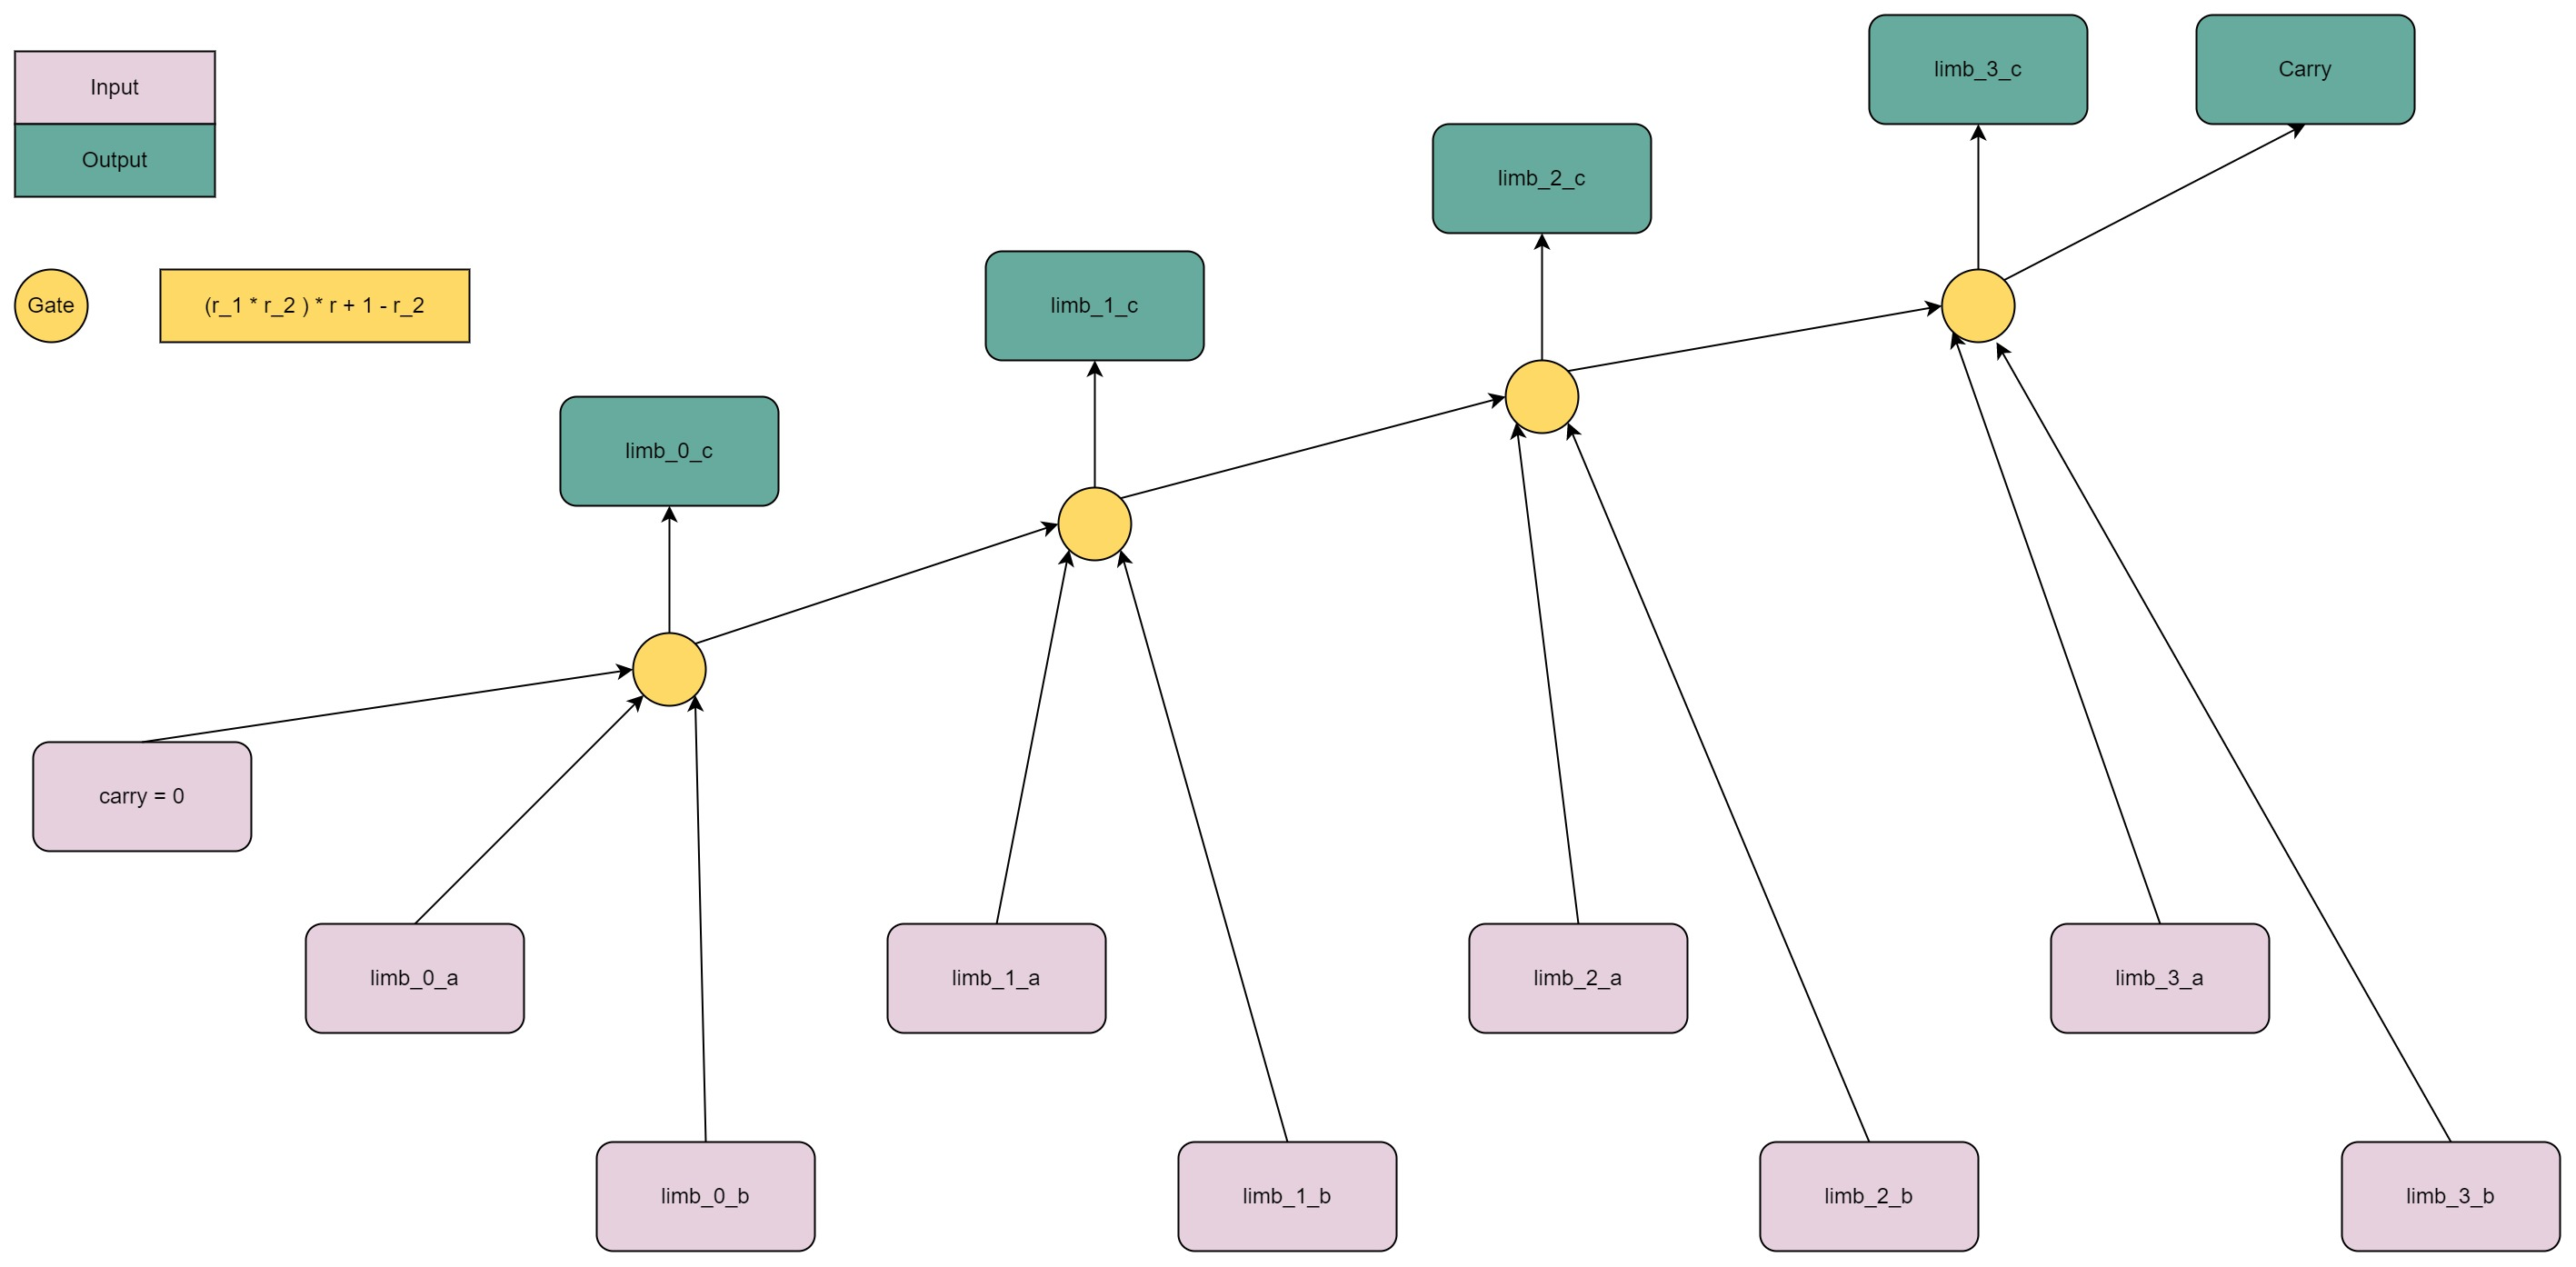
\includegraphics[width=0.8\textwidth]{biguint-add-circuit-layout.jpg}
    \caption{biguint-add circuit layout}
    \label{fig:biguint-add-circuit-layout}
\end{figure}

\Par{Trace layout}
See \figref{fig:biguint-add-trace-layout}.
\begin{figure}[!ht]
    \centering
    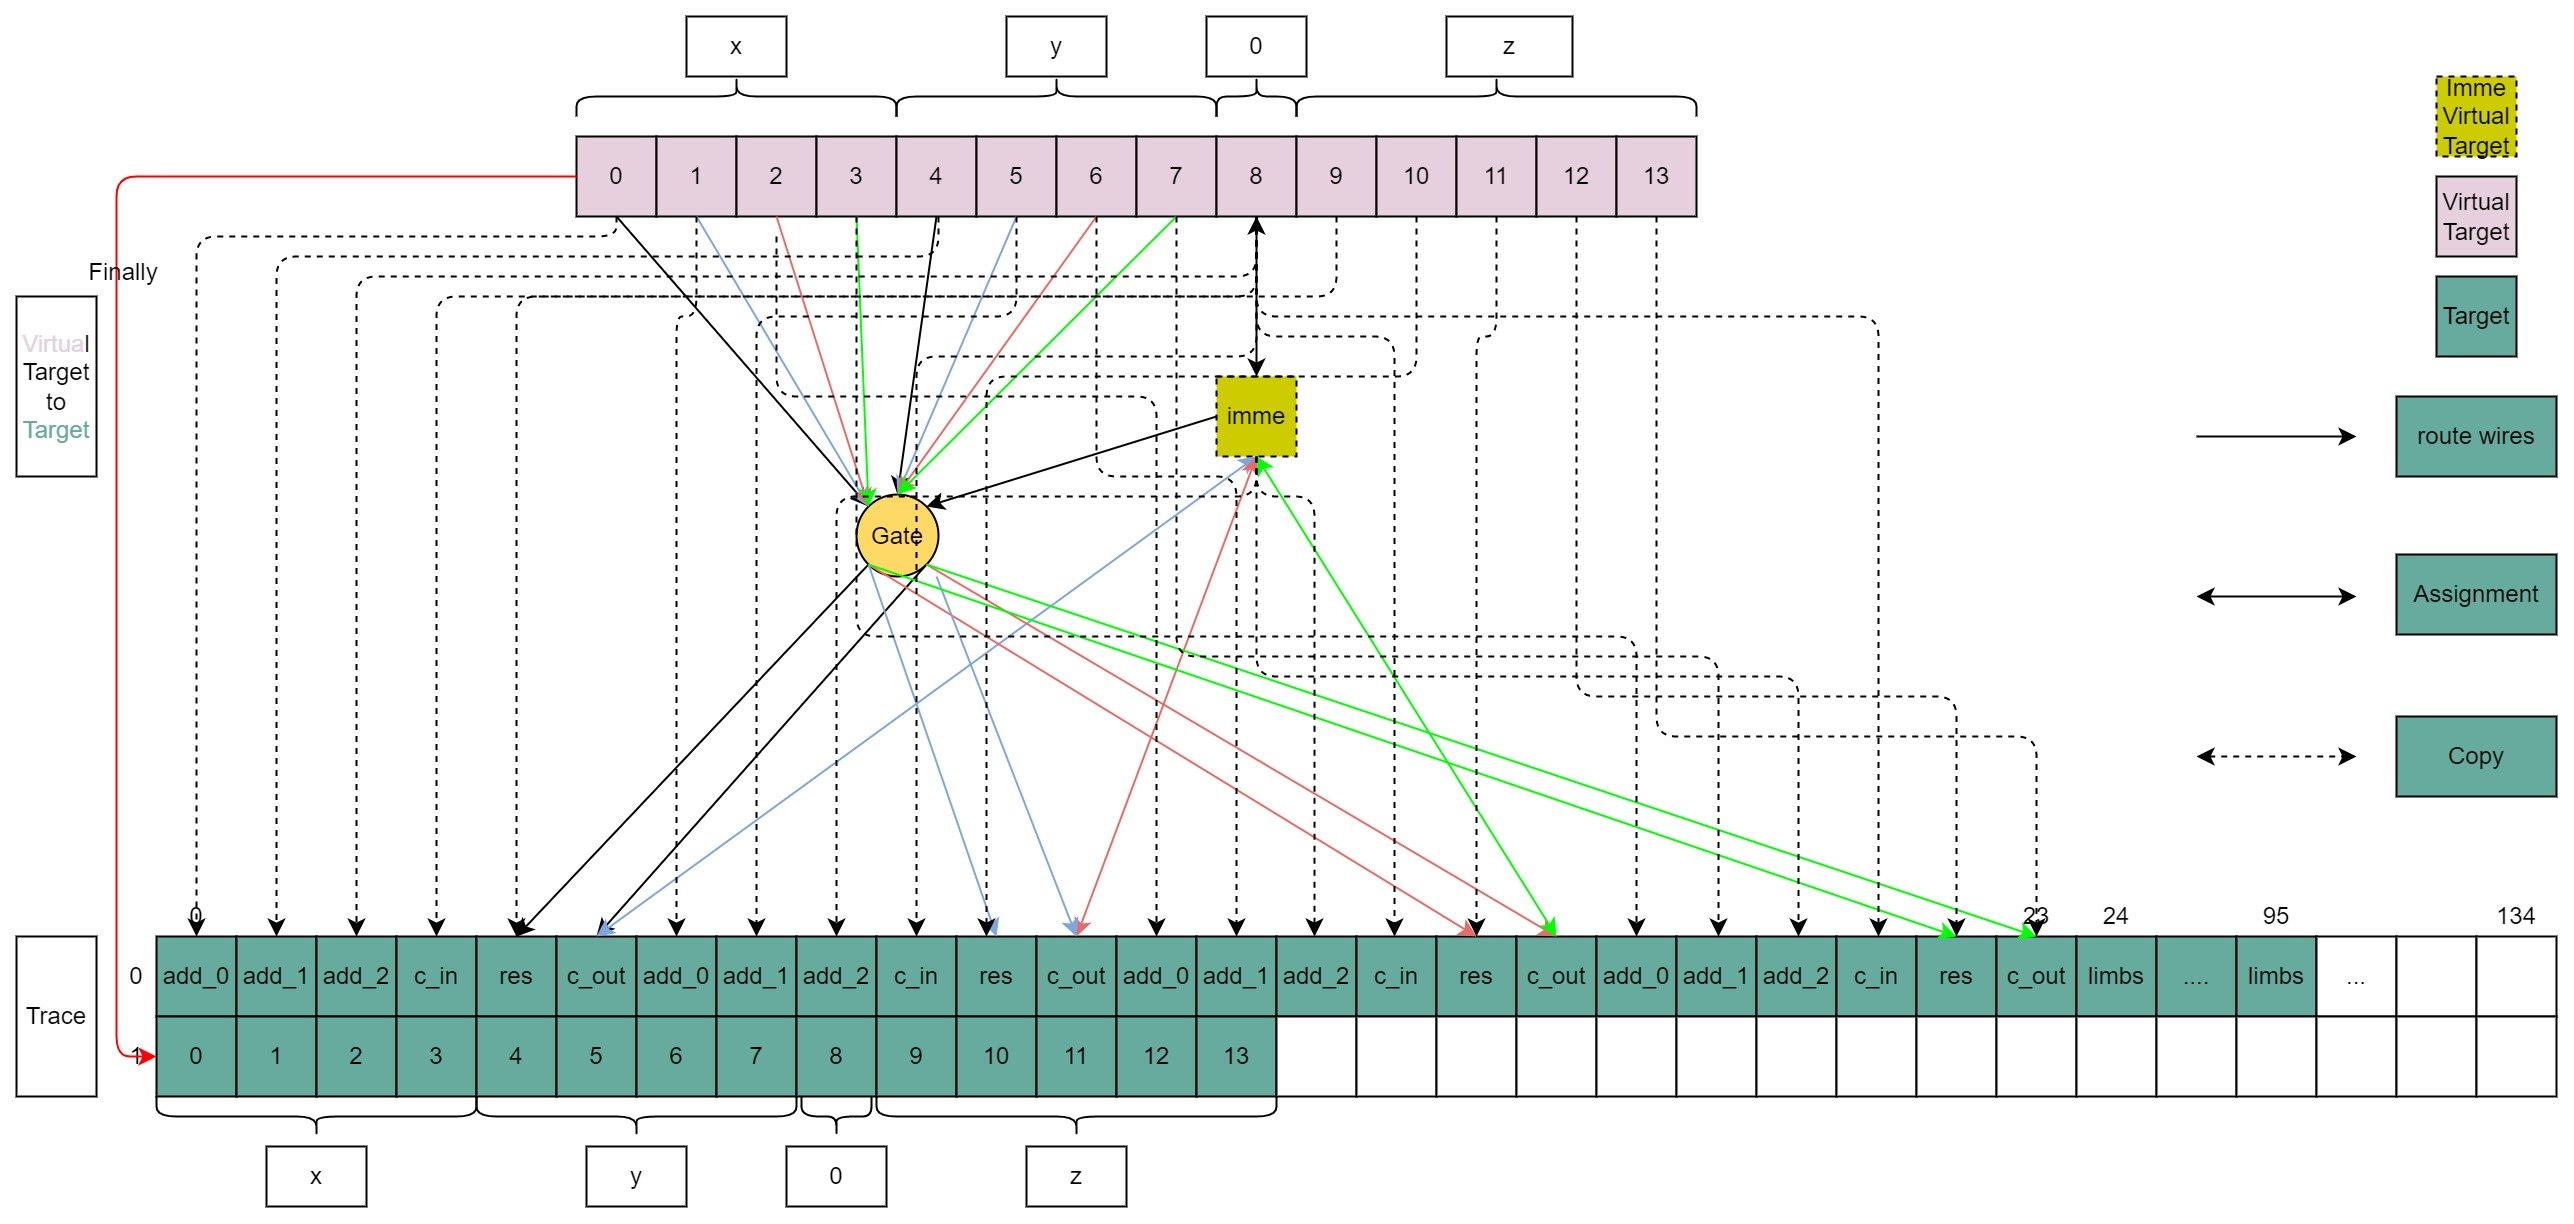
\includegraphics[width=0.8\textwidth]{biguint-add-trace-layout.jpg}
    \caption{biguint-add trace layout}
    \label{fig:biguint-add-trace-layout}
\end{figure}

\Par{Constraints info and costs}
\begin{itemize}
    \item gate type num: 1 (U32AddManyGate)
    \item gate ops num: limbs-num
    \item gate instance num: ceil(limbs-num / gate.ops)
    \item copy-constraints: limbs-num * 4
    \item max-degree: 4 (\verb|1 << limb-bits|)
\end{itemize}

\Par{Questions}
\begin{itemize}
    \item Why not make rangecheck constraint for inputs?
    \item Why not make copy constraint between cur-c-in and last-c-out?
\end{itemize}

    \subsubsection{biguint-sub}

\Par{Target}
Implement the substraction of two biguints.

\Par{Constraints logic}
\begin{itemize}
    \item Equation for gate;
    \item Sumcheck for ouptput;
    \item Rangecheck for limbs.
\end{itemize}

\Par{Circuit layout}
See \figref{fig:biguint-sub-circuit-layout}.
\begin{figure}[!ht]
    \centering
    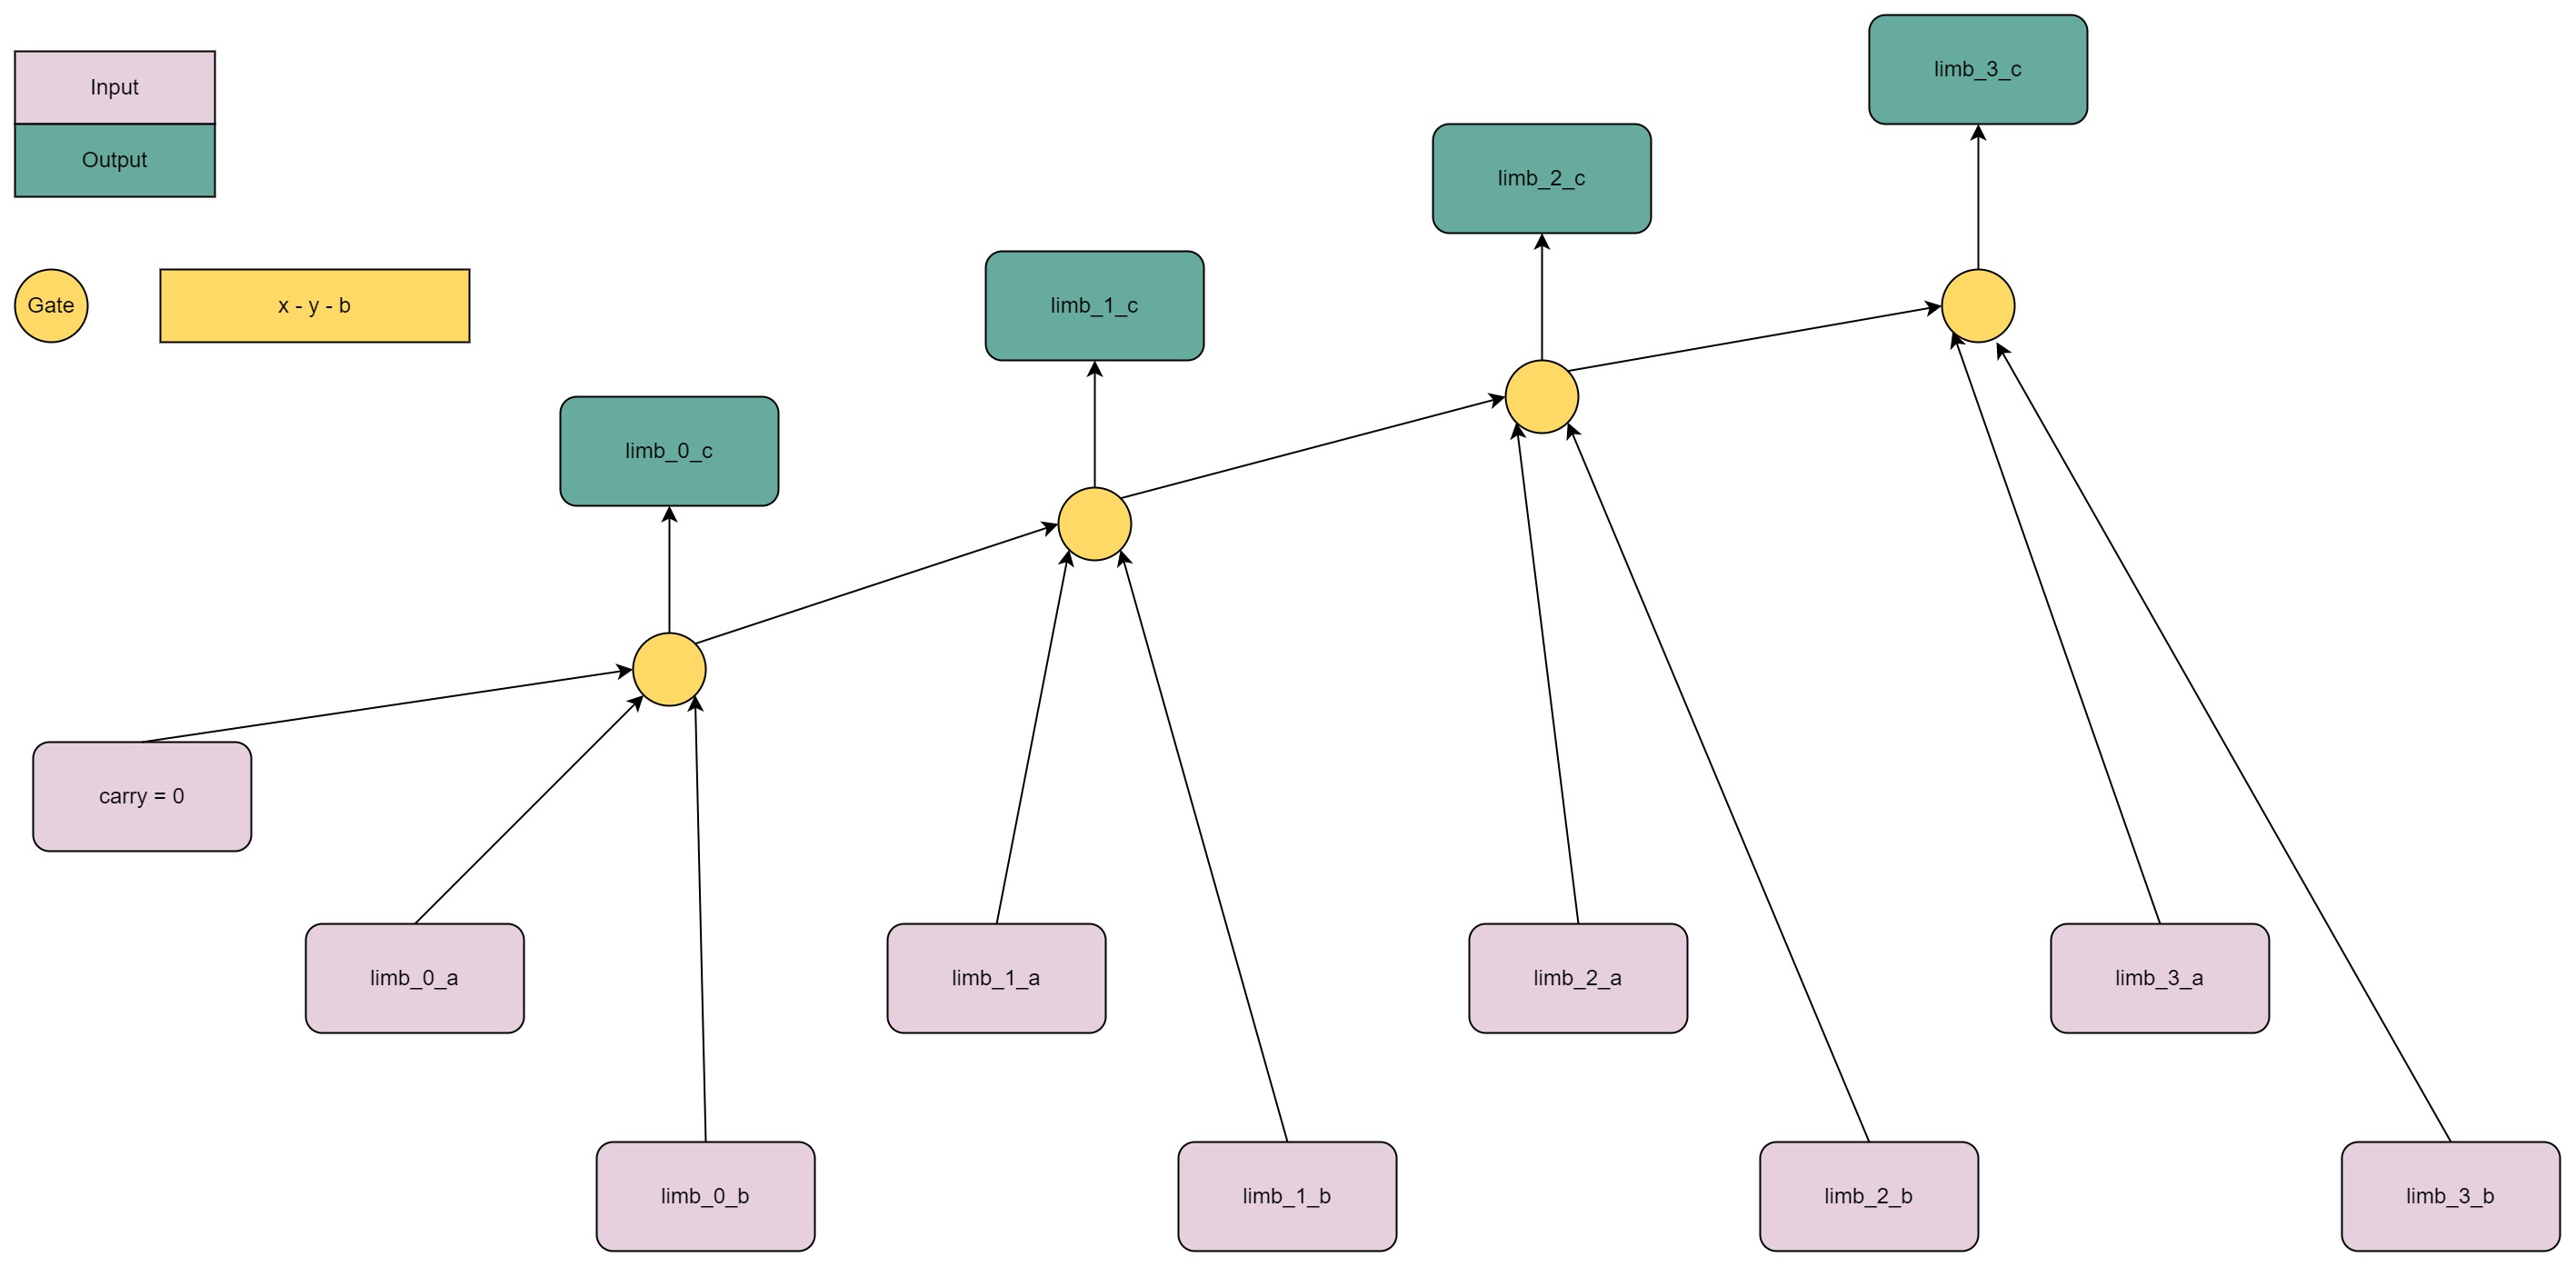
\includegraphics[width=0.8\textwidth]{biguint-sub-circuit-layout.jpg}
    \caption{biguint-sub circuit layout}
    \label{fig:biguint-sub-circuit-layout}
\end{figure}

\Par{Trace layout}
See \figref{fig:biguint-sub-trace-layout}.
\begin{figure}[!ht]
    \centering
    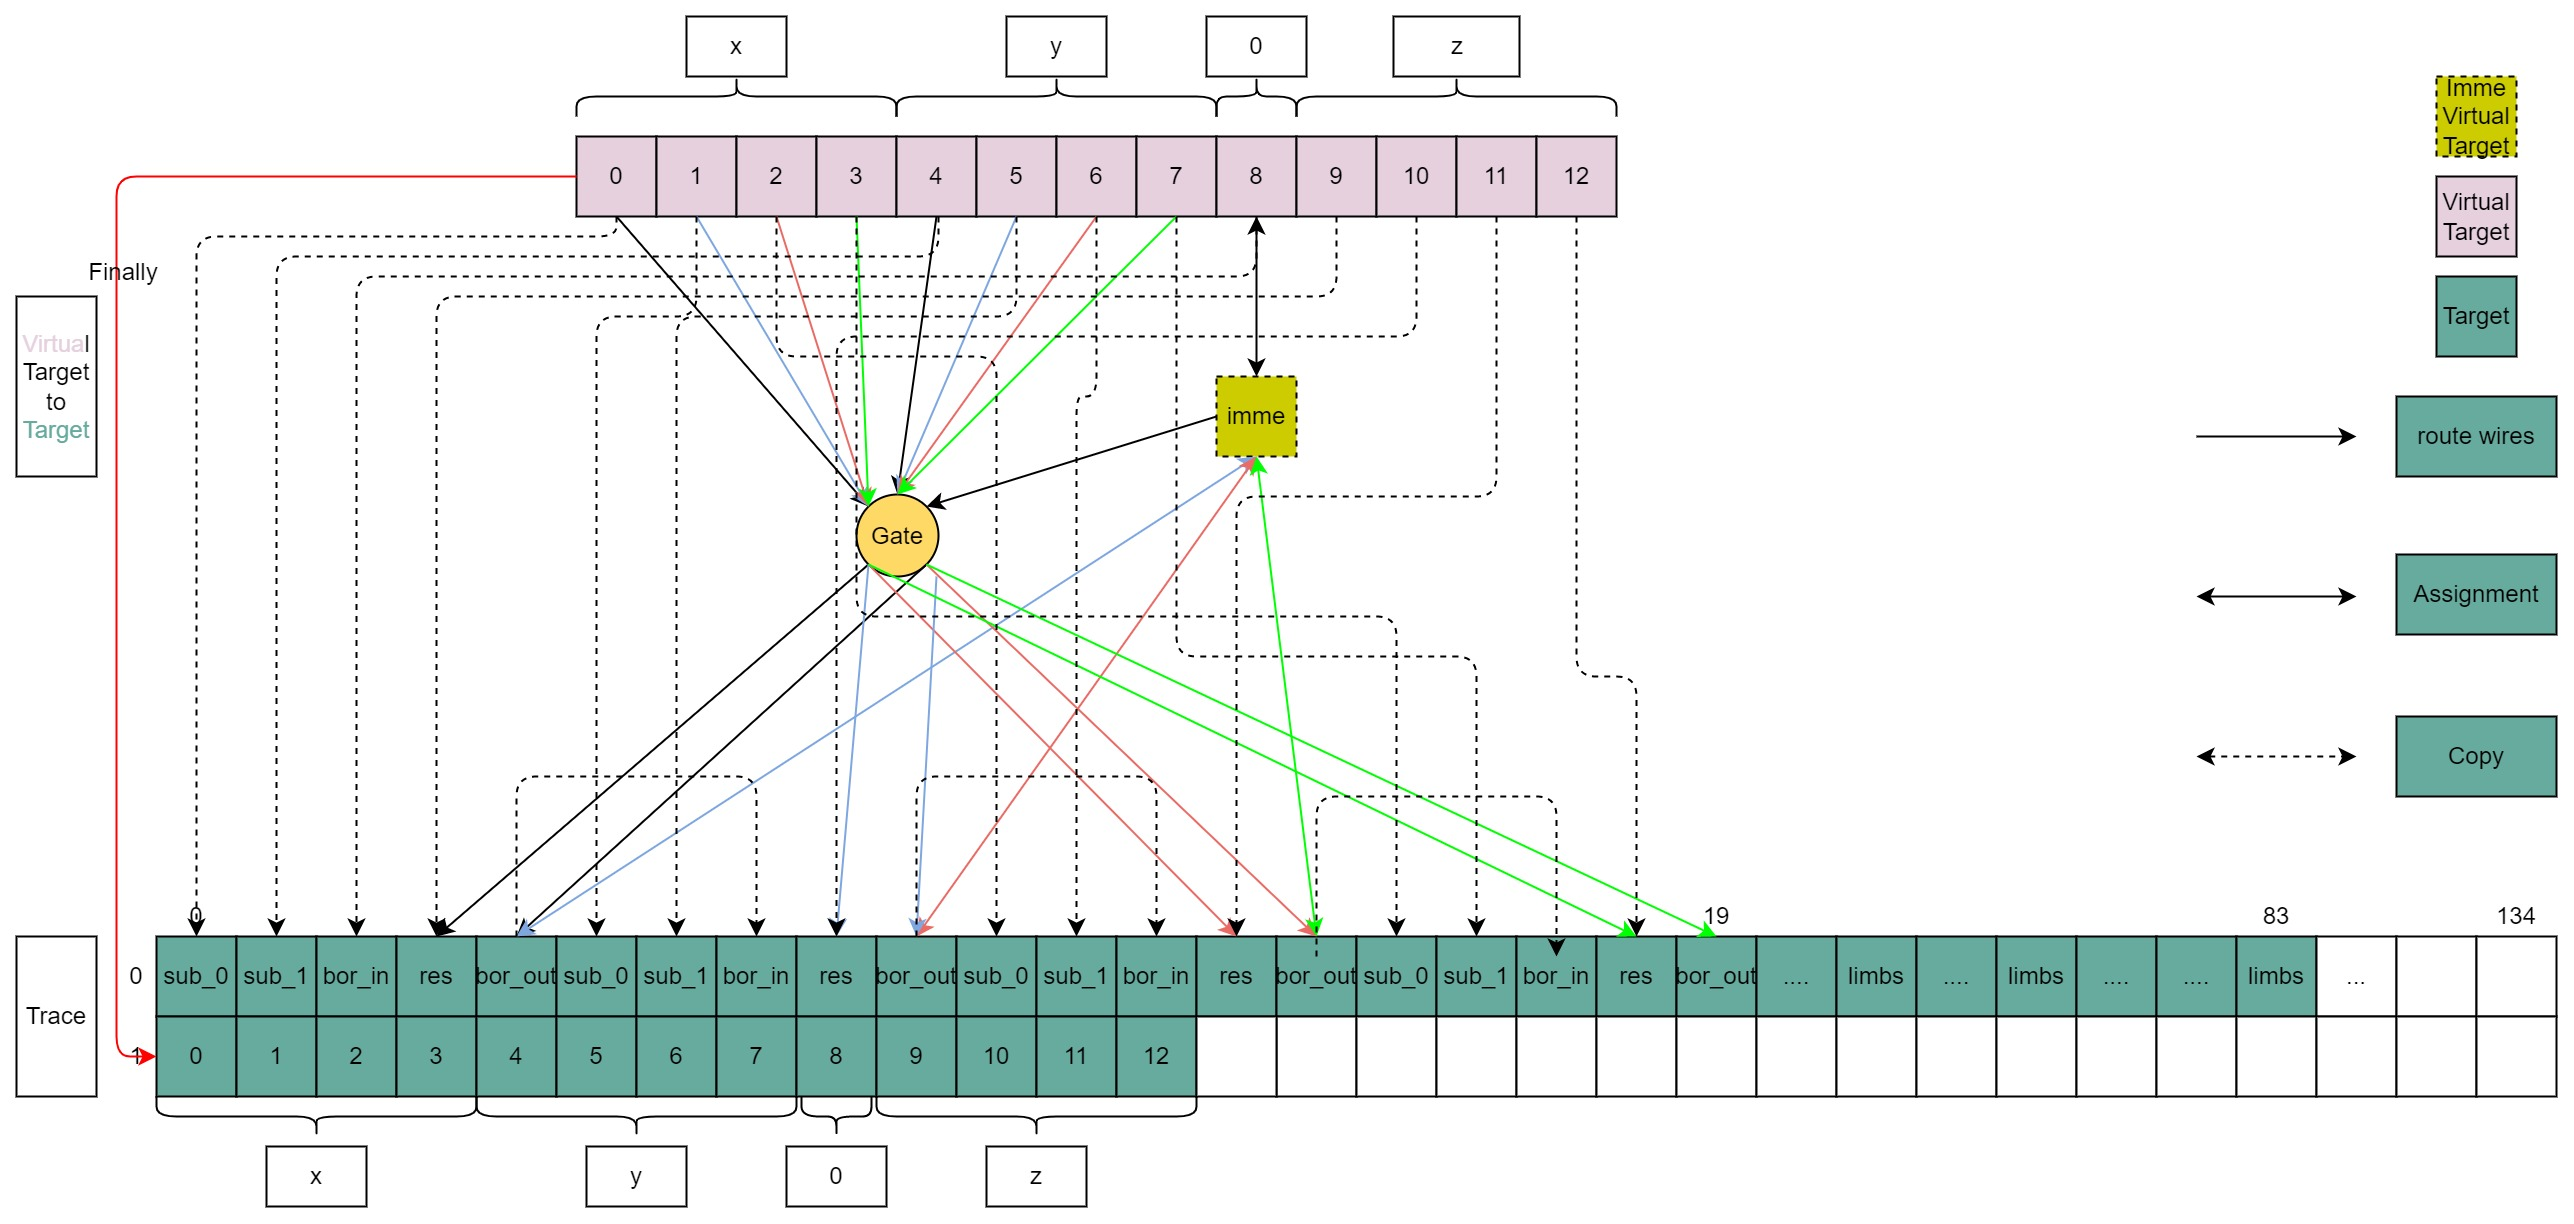
\includegraphics[width=0.8\textwidth]{biguint-sub-trace-layout.jpg}
    \caption{biguint-sub trace layout}
    \label{fig:biguint-sub-trace-layout}
\end{figure}

\Par{Constraints info and costs}
\begin{itemize}
    \item constraints-num: $6 \times (3 + 32 / 2) = 114$
    \item copy-constraints: $16$
    \item max-degree: $4$
    \item wires-num: $6 \times (5 + 16) = 126$
\end{itemize}

\Par{Questions}
\begin{itemize}
    \item Why not make rangecheck constraint for inputs?
    \item Could try to use the same constraint with add-gate.
\end{itemize}

    \subsubsection{biguint-mul}

\Par{Target}
Implement the multiplication of two biguints.

\Par{Constraints logic}
\begin{itemize}
    \item Compute mul-factors first, use U32ArithmeticGate;
    \item Add mul-factors from low bits, use U32AddManyGate.
\end{itemize}

\Par{Process layout}
See \figref{fig:biguint-mul-layout}
\begin{figure}[!ht]
    \centering
    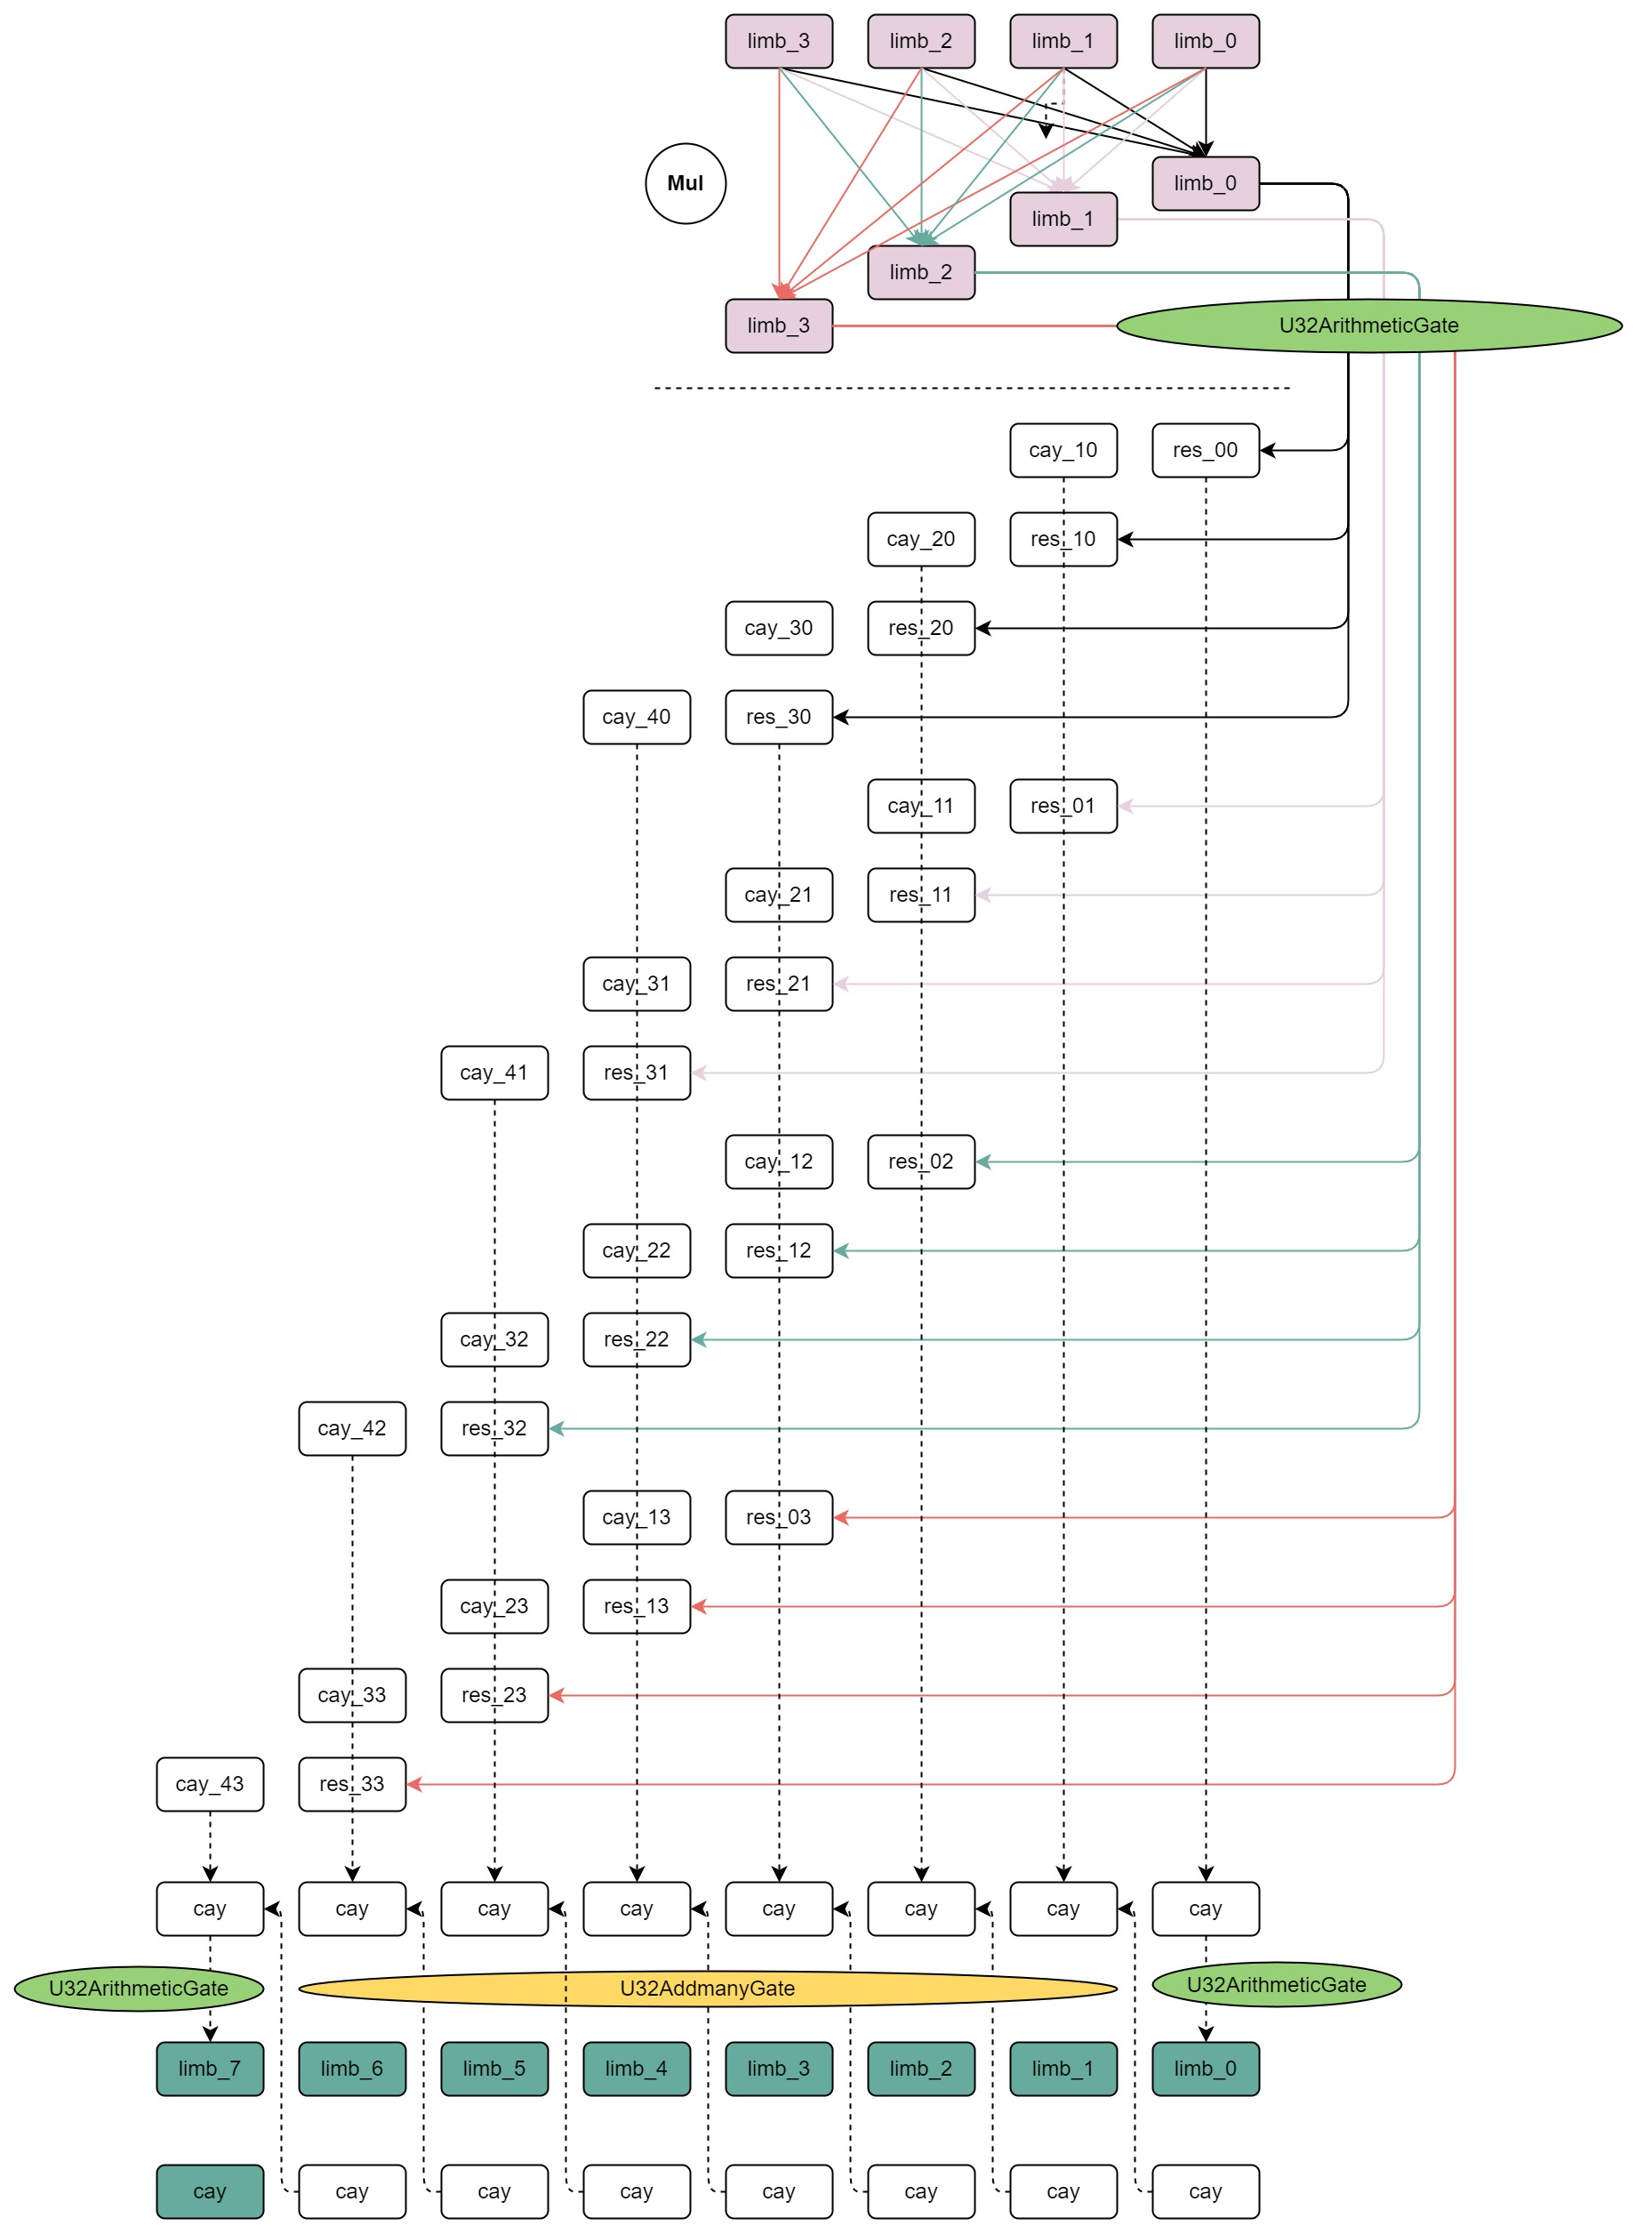
\includegraphics[width=0.8\textwidth]{biguint-mul-layout.jpg}
    \caption{biguint-mul layout}
    \label{fig:biguint-mul-layout}
\end{figure}

\Par{Constraints info and costs}
\begin{itemize}
    \item Gate type num: 4 (U32ArithmeticGate, U32AddManyGate(num-addends: 4), U32AddManyGate(num-addends: 6), U32AddManyGate(num-addends: 8))
    \item Gate instance num: 9
    \item U32ArithmeticGate num: 6
    \item U32AddManyGate num: 3
    \item copy-constraints: $18 \times 3 + (4 + 6 + 8) \times 2 + 9 = 99$
    \item max-degree: 4
\end{itemize}

    \section{biguint-div}
\label{biguint-div}

Note that div-rem has the same constraints logic with div

\begin{enumerate}
    \item target
        \begin{itemize}
            \item implement the division of two biguints
        \end{itemize}
    \item constraints-logic
        \begin{itemize}
            \item not implement div-algrithem directly
            \item use nondeterministic feature to check div-logic
            \item check div * b + rem = a
            \item check rem < b
        \end{itemize}
    \item div-process layout
        \begin{figure}[!ht]
            \centering
            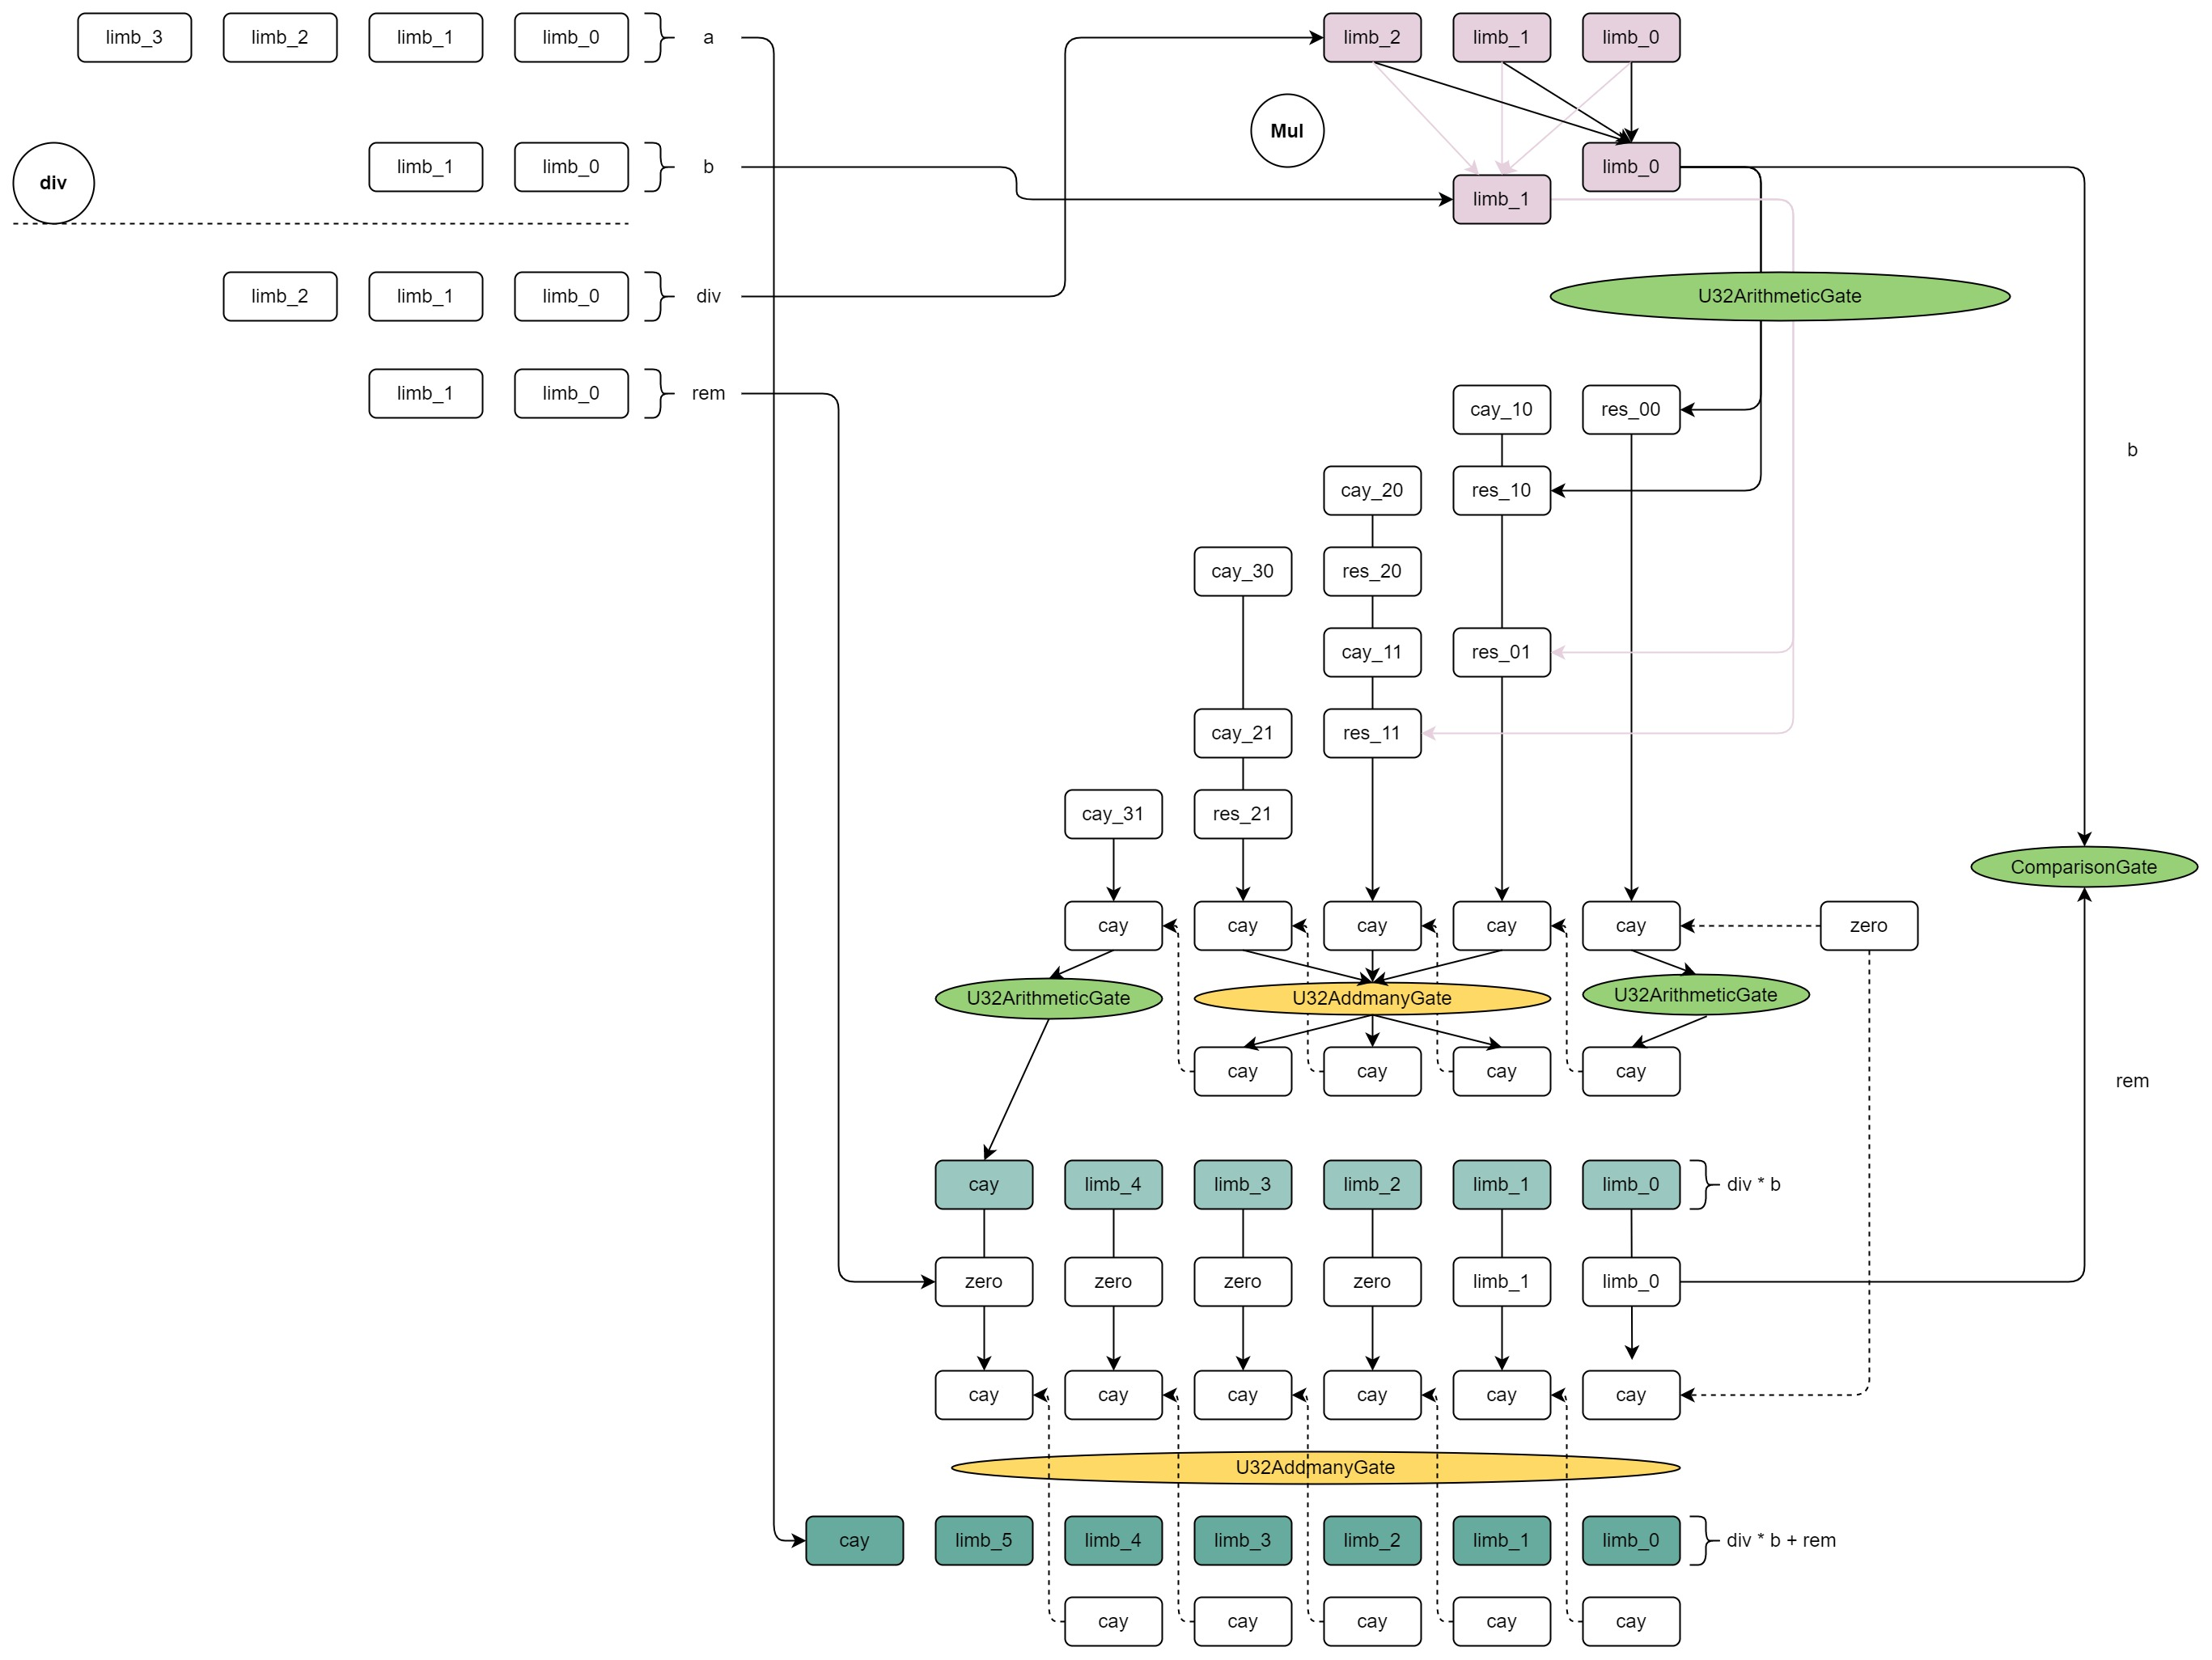
\includegraphics[width=0.8\textwidth]{biguint-div-layout.jpg}
            \caption{biguint-div layout.jpg}
            \label{fig:biguint-div-layout.jpg}
        \end{figure}
    
    \item constraints-info and costs
        \begin{itemize}
            \item Gate type num: 5(U32ArithmeticGate, U32AddManyGate(num-addends: 3), U32AddManyGate(num-addends: 4), ComparisionGate, ArithmeticGate)
            \item Gate instance num: 3 + 3 + 4 + 3 = 13 
            \item U32ArithmeticGate num: 3
            \item U32AddManyGate num: 3
            \item ComparisionGate num: 4
            \item ArithmeticGate num: 3
            \item copy-constraints: 3 * 8 + 4 + 5 + 4 + 4 * 6 + 7 + 1 + 26 + 5 = 100 
            \item max-degree: 4
        \end{itemize}

\end{enumerate}
    \subsubsection{biguint-cmp}

\Par{Target}
Implement the comparison of two biguints.

\Par{Constraints logic}
\begin{itemize}
    \item Split the input to many limbs, such that: \verb|limbs_num = bits / chunks|;
    \item Execute comparison for low bits limbs;
    \item Ensure that the result is determined by the highest limbs which are not equal.
\end{itemize}

\Par{Process layout}
See \figref{fig:biguint-cmp-layout}.
\begin{figure}[!ht]
    \centering
    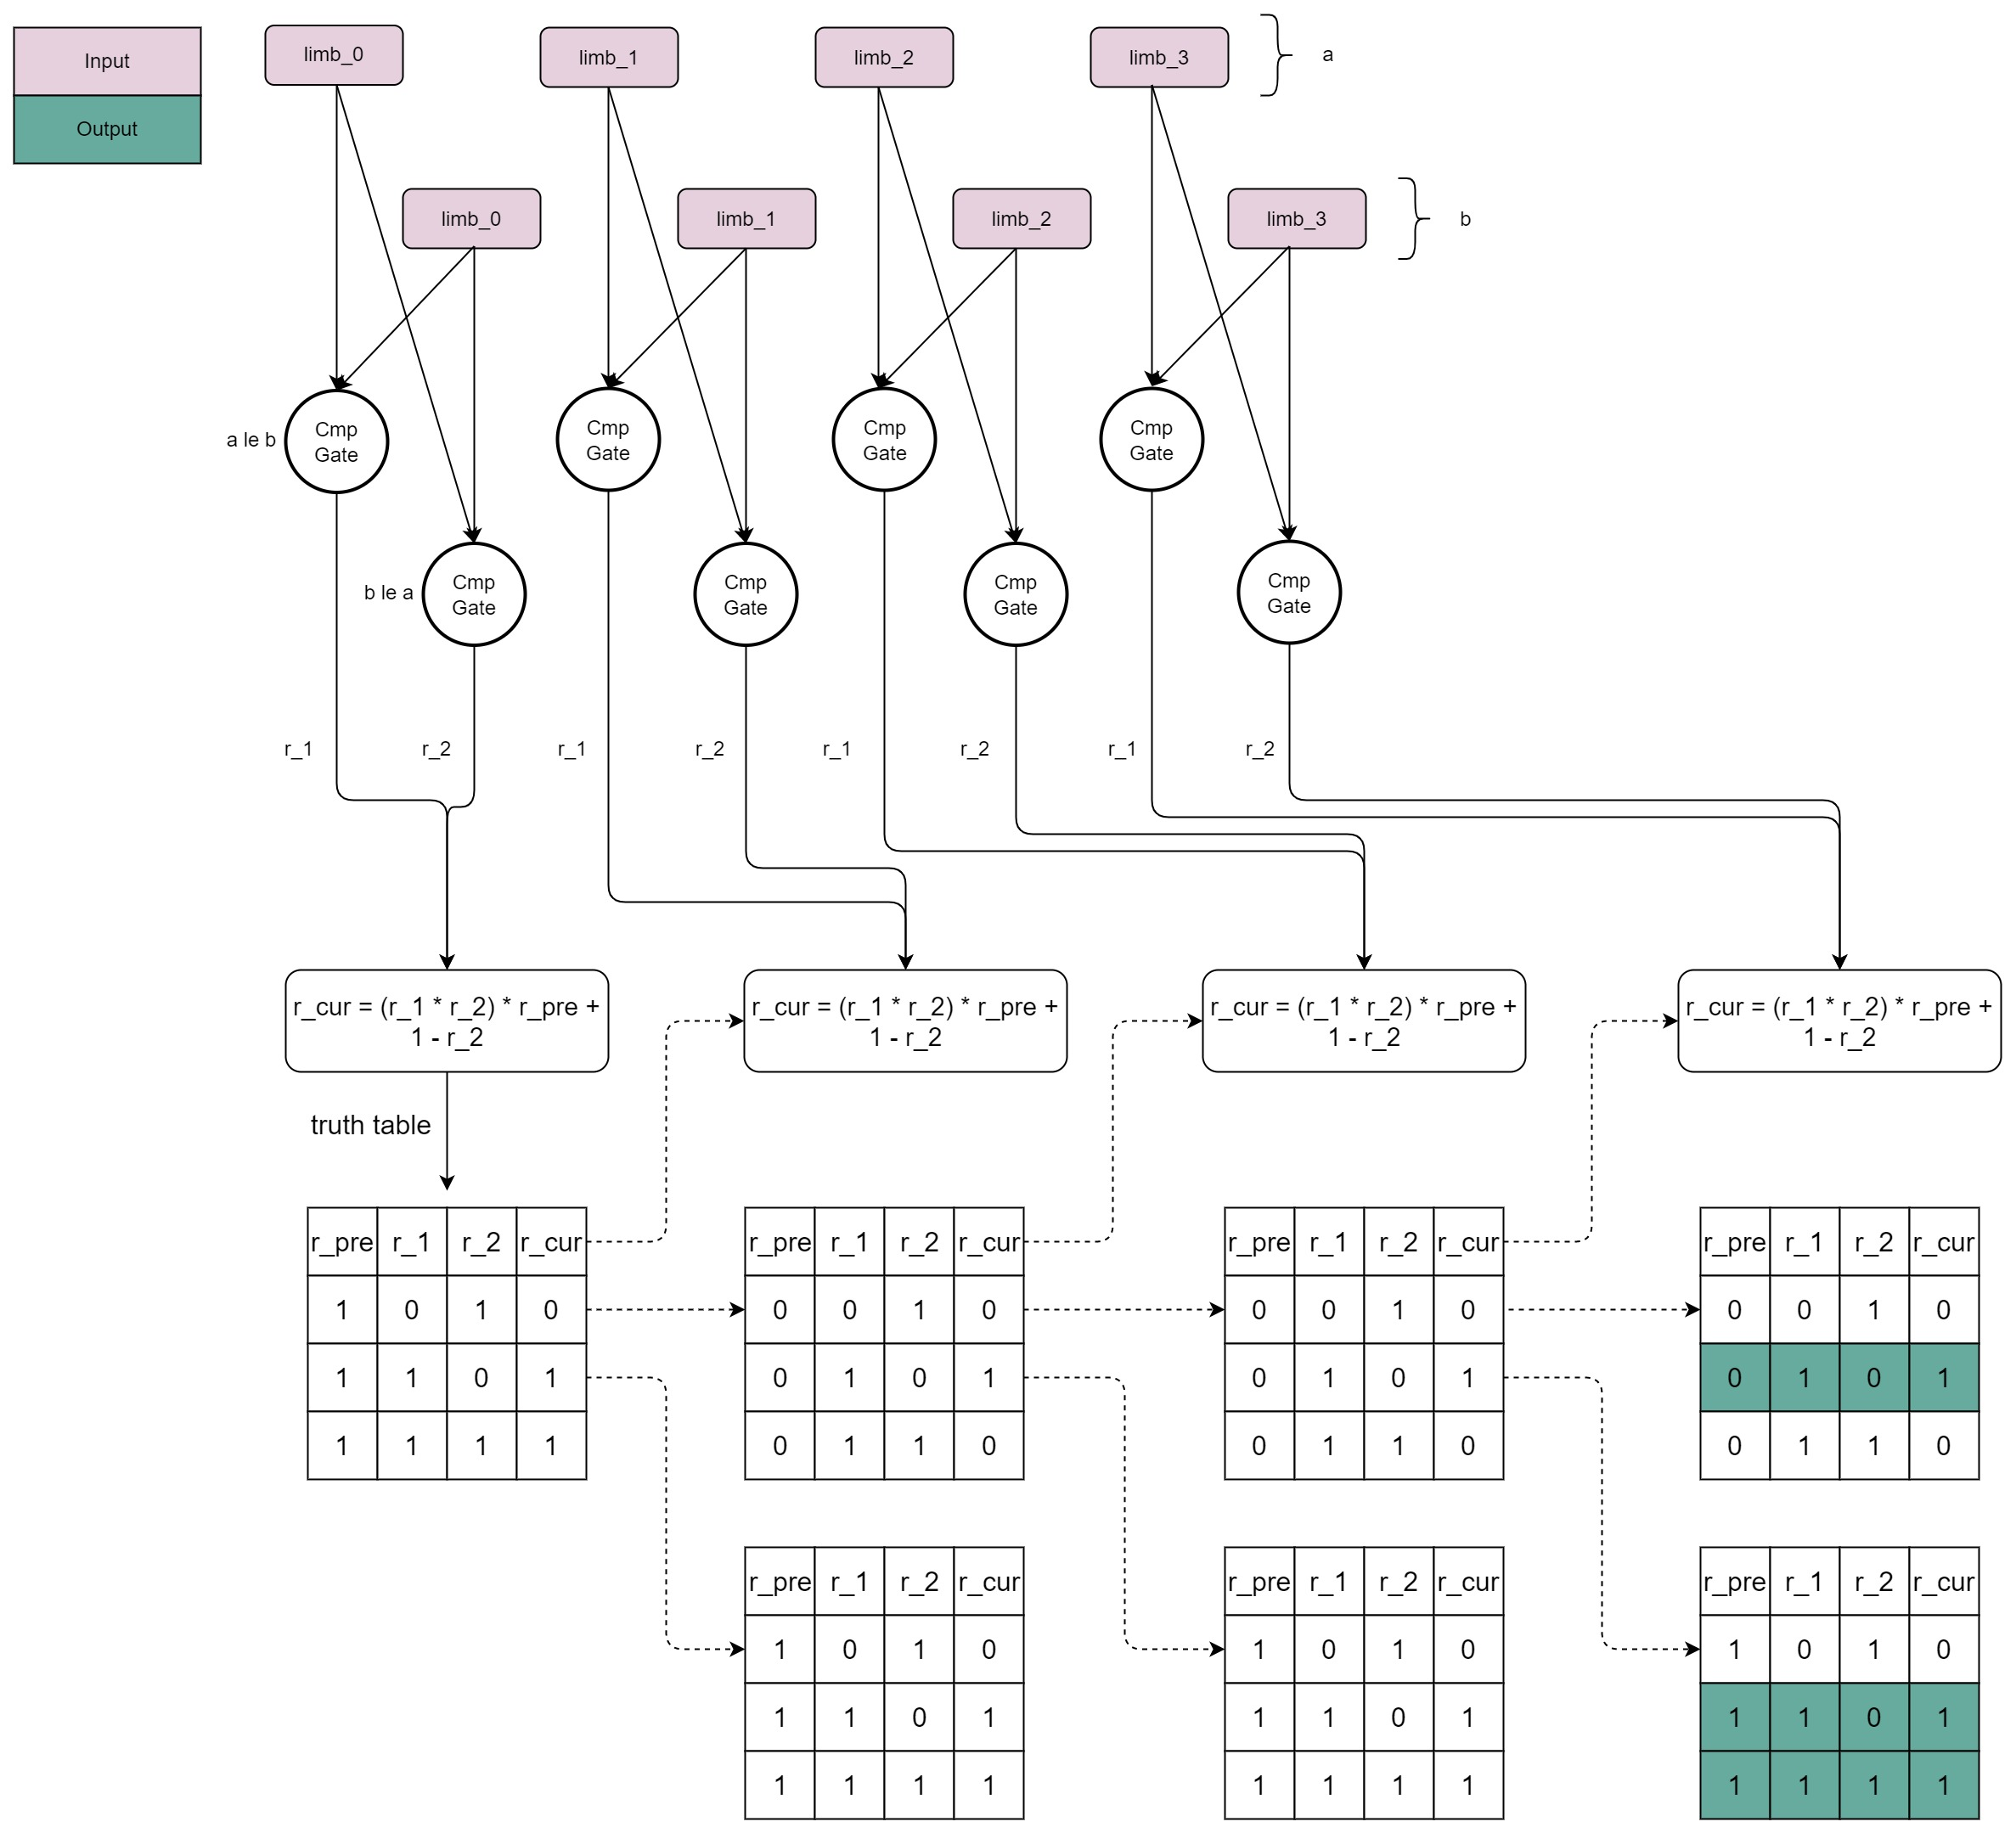
\includegraphics[width=0.8\textwidth]{biguint-cmp-layout.jpg}
    \caption{biguint-cmp layout}
    \label{fig:biguint-cmp-layout}
\end{figure}

\Par{Circuit layout}
See \figref{fig:biguint-cmp-circuit-layout}.
\begin{figure}[!ht]
    \centering
    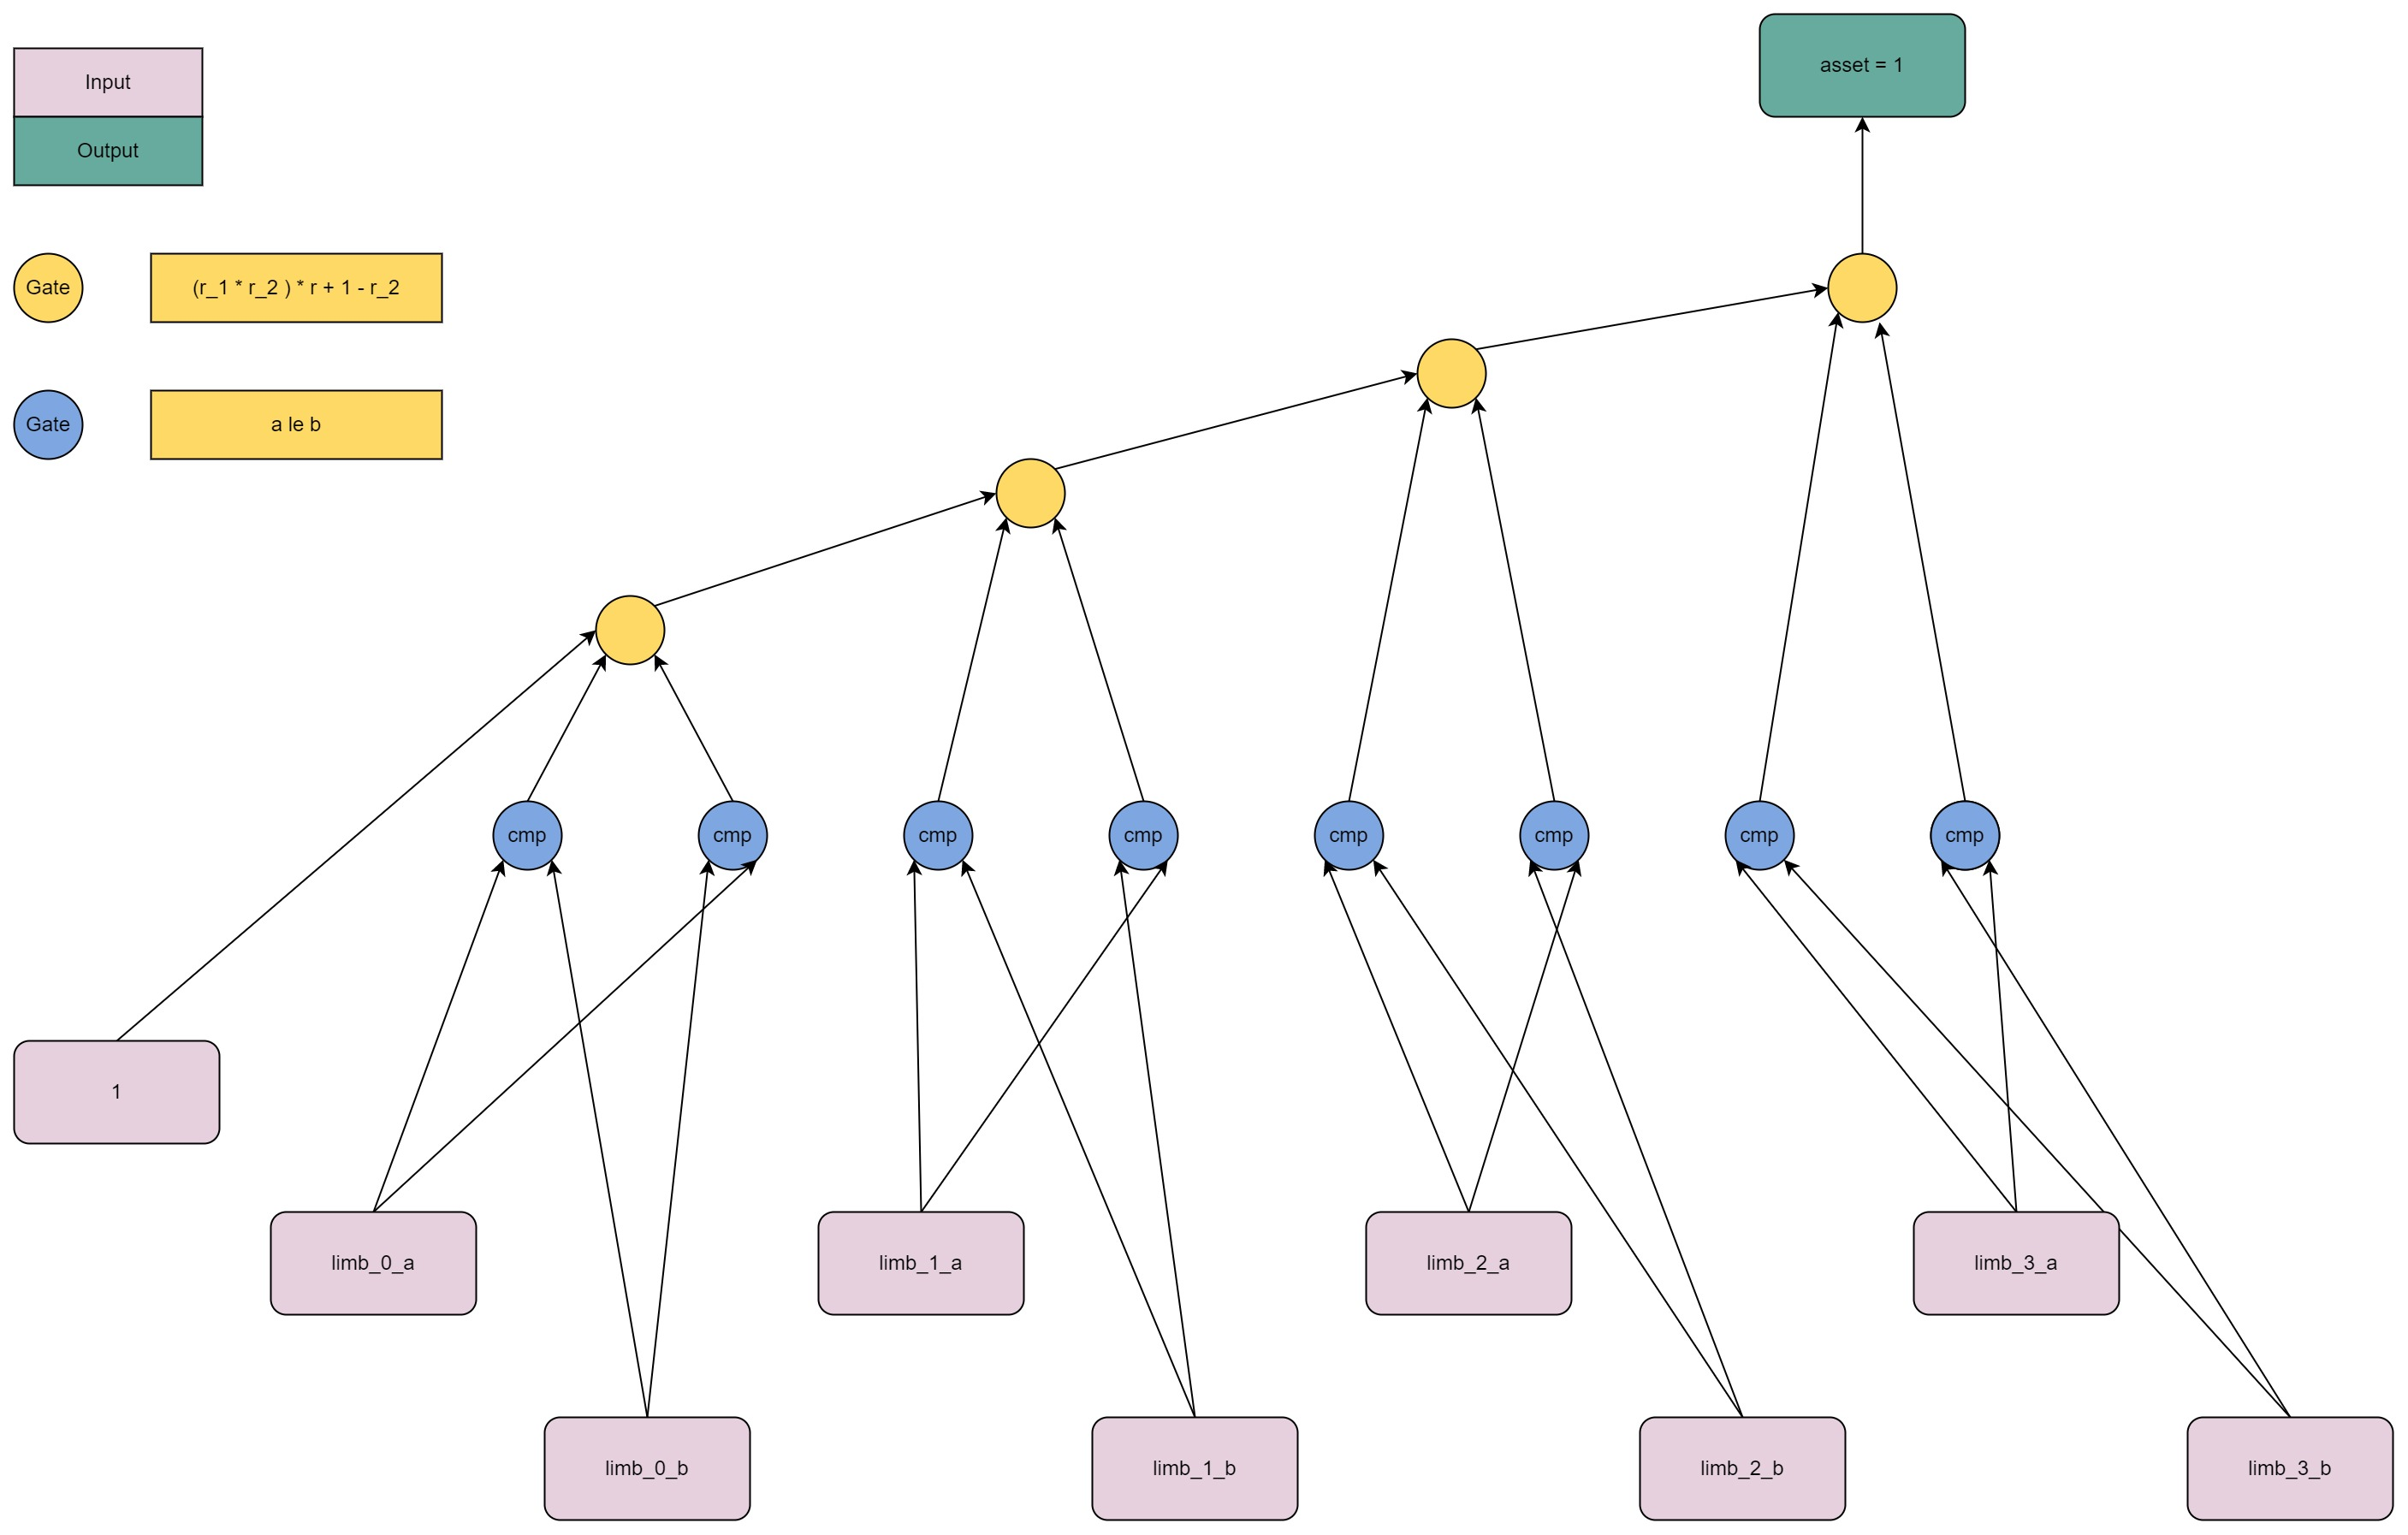
\includegraphics[width=0.8\textwidth]{biguint-cmp-circuit-layout.jpg}
    \caption{biguint-cmp circuit layout}
    \label{fig:biguint-cmp-circuit-layout}
\end{figure}

\Par{Constraints info and costs}
\begin{itemize}
    \item Gate type num: 2 (ComparisionGate, ArithmeticGate)
    \item Gate instance num: $4 \times 2 + 3 = 11$
    \item ComparisionGate num: 8
    \item ArithmeticGate num: 3
    \item copy-constraints: $(4 + 9) \times 4 + 1 = 53$
    \item max-degree: 4
\end{itemize}

    \subsubsection{nonnative-add}
\label{nonnative-add}

\begin{enumerate}
    \item target
        check the additional relation among three nonnative target objects.
    \item constraints-logic
        \begin{itemize}
            \item check equation for gadget,  a + b = c + modular * overflow
            \item check that "c lt modular"
        \end{itemize}
    \item nonnative-add process layout
        \begin{figure}[!ht]
            \centering
            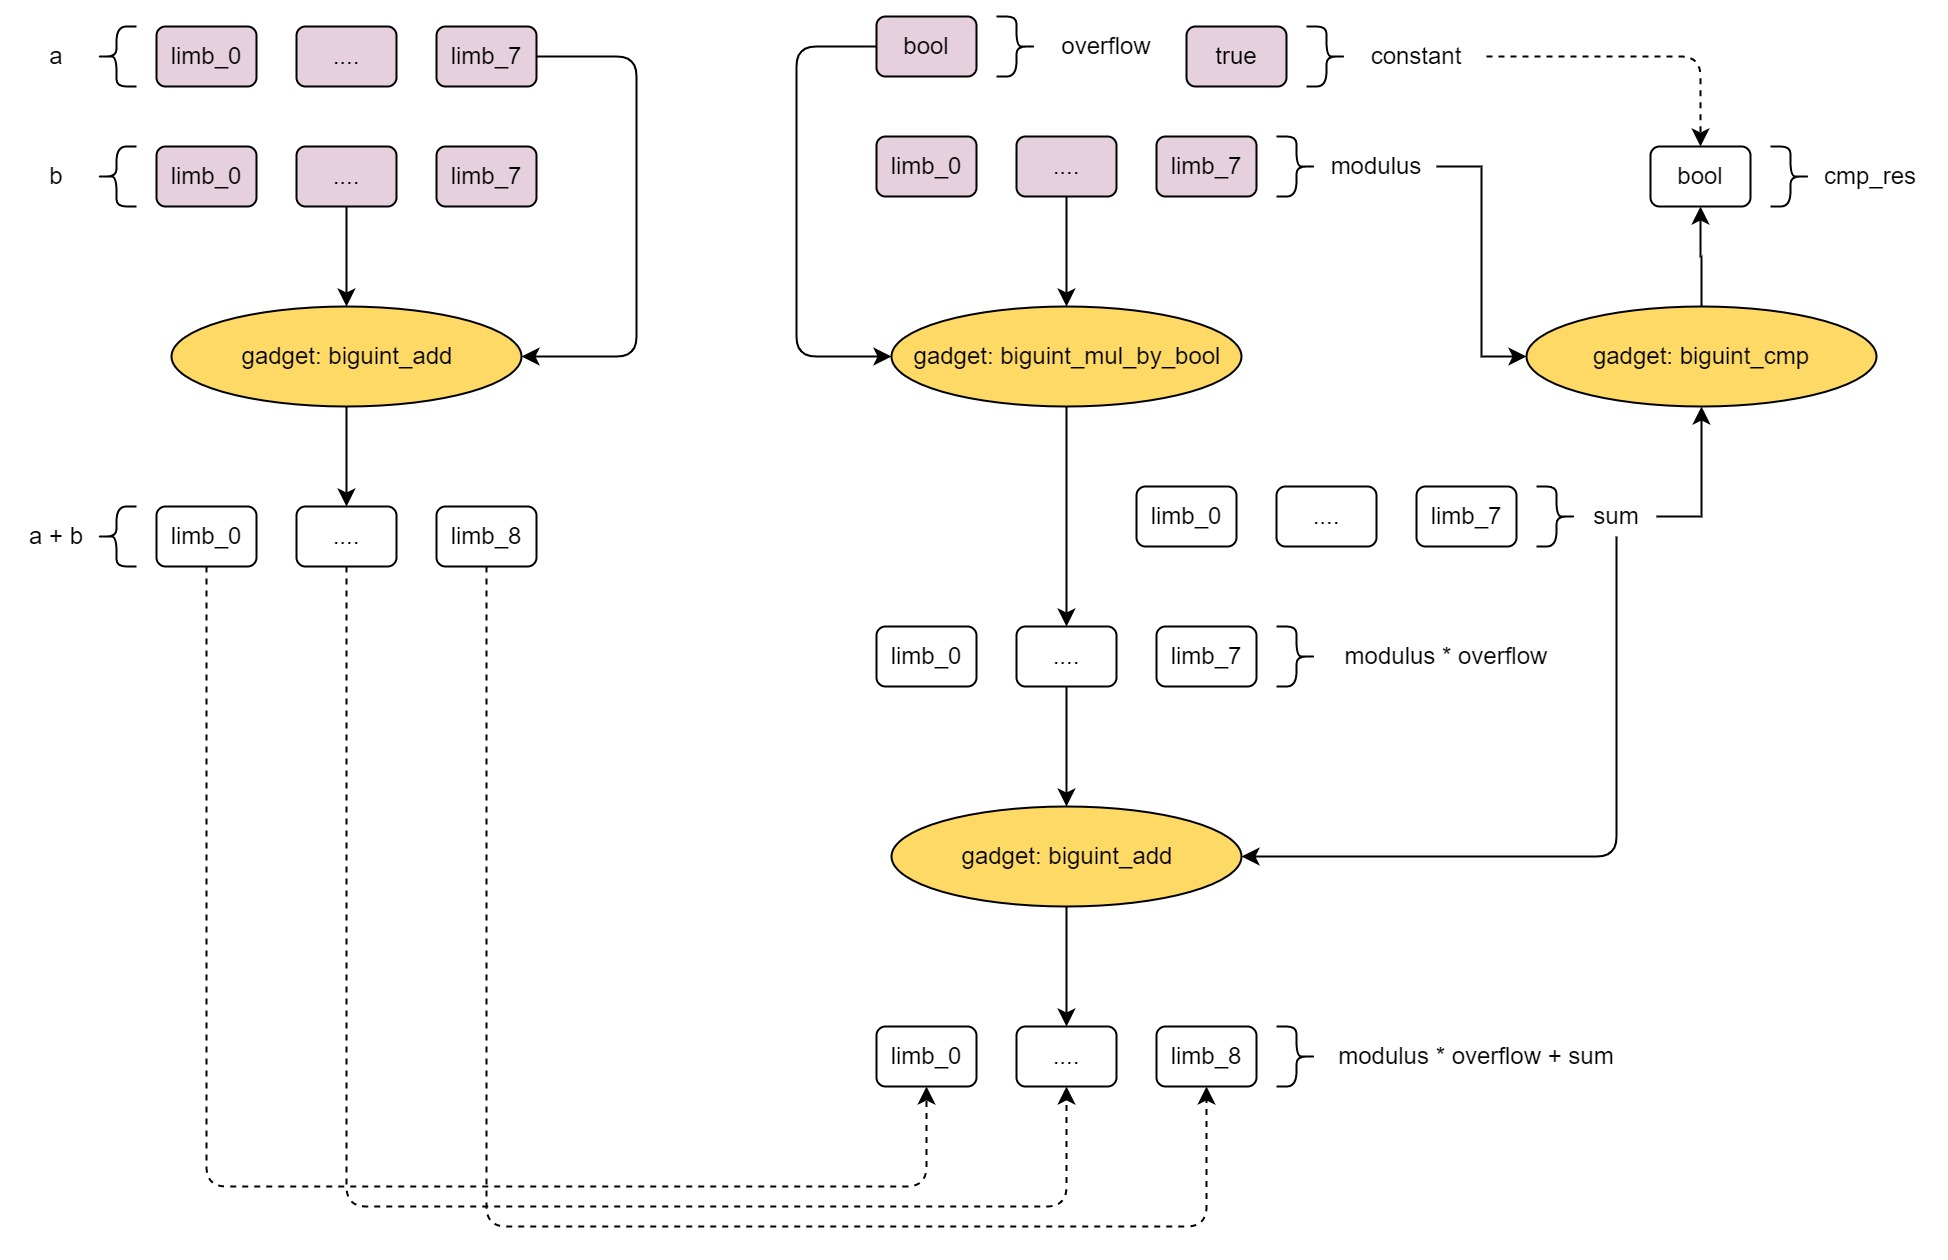
\includegraphics[width=0.8\textwidth]{nonnative-add-layout.jpg}
            \caption{nonnative-add layout}
            \label{fig:nonnative-add-layout}
        \end{figure}
    
    \item constraints-info and costs
        \begin{itemize}
            \item gadget biguint-add num: 2
            \item gadget biguint-mul-by-bool num: 1
            \item gadget biguint-cmp num: 1
            \item gate type num: 3(U32AddManyGate, ComparisonGate, ArithmeticGate)
            \item gate instance num: 23 = 3(U32AddManyGate) + 16(ComparisonGate) + 2(ArithmeticGate(1,0)) + 1(ArithmeticGate(1,-1)) + 1(ArithmeticGate(1,1))
            \item copy-constraints: 186 = 32 * 2{biguint-add} + 9{biguint-mul-by-bool} + 9 + (4 + 9) * 8{biguint-cmp} = 186
        \end{itemize}

    \item questions
        \begin{itemize}
            \item when set value to sum?
        \end{itemize}

\end{enumerate}
    \subsubsection{nonnative-sub}
\label{nonnative-sub}

\begin{enumerate}
    \item target
        check the substract relation among three nonnative target objects.
    \item constraints-logic
        \begin{itemize}
            \item check equation for gadget,  diff + b = a + modular * overflow
            \item check that "overflow is bool"
            \item check that "diff.limbs is range U32"
        \end{itemize}
    \item nonnative-sub process layout
        \begin{figure}[!ht]
            \centering
            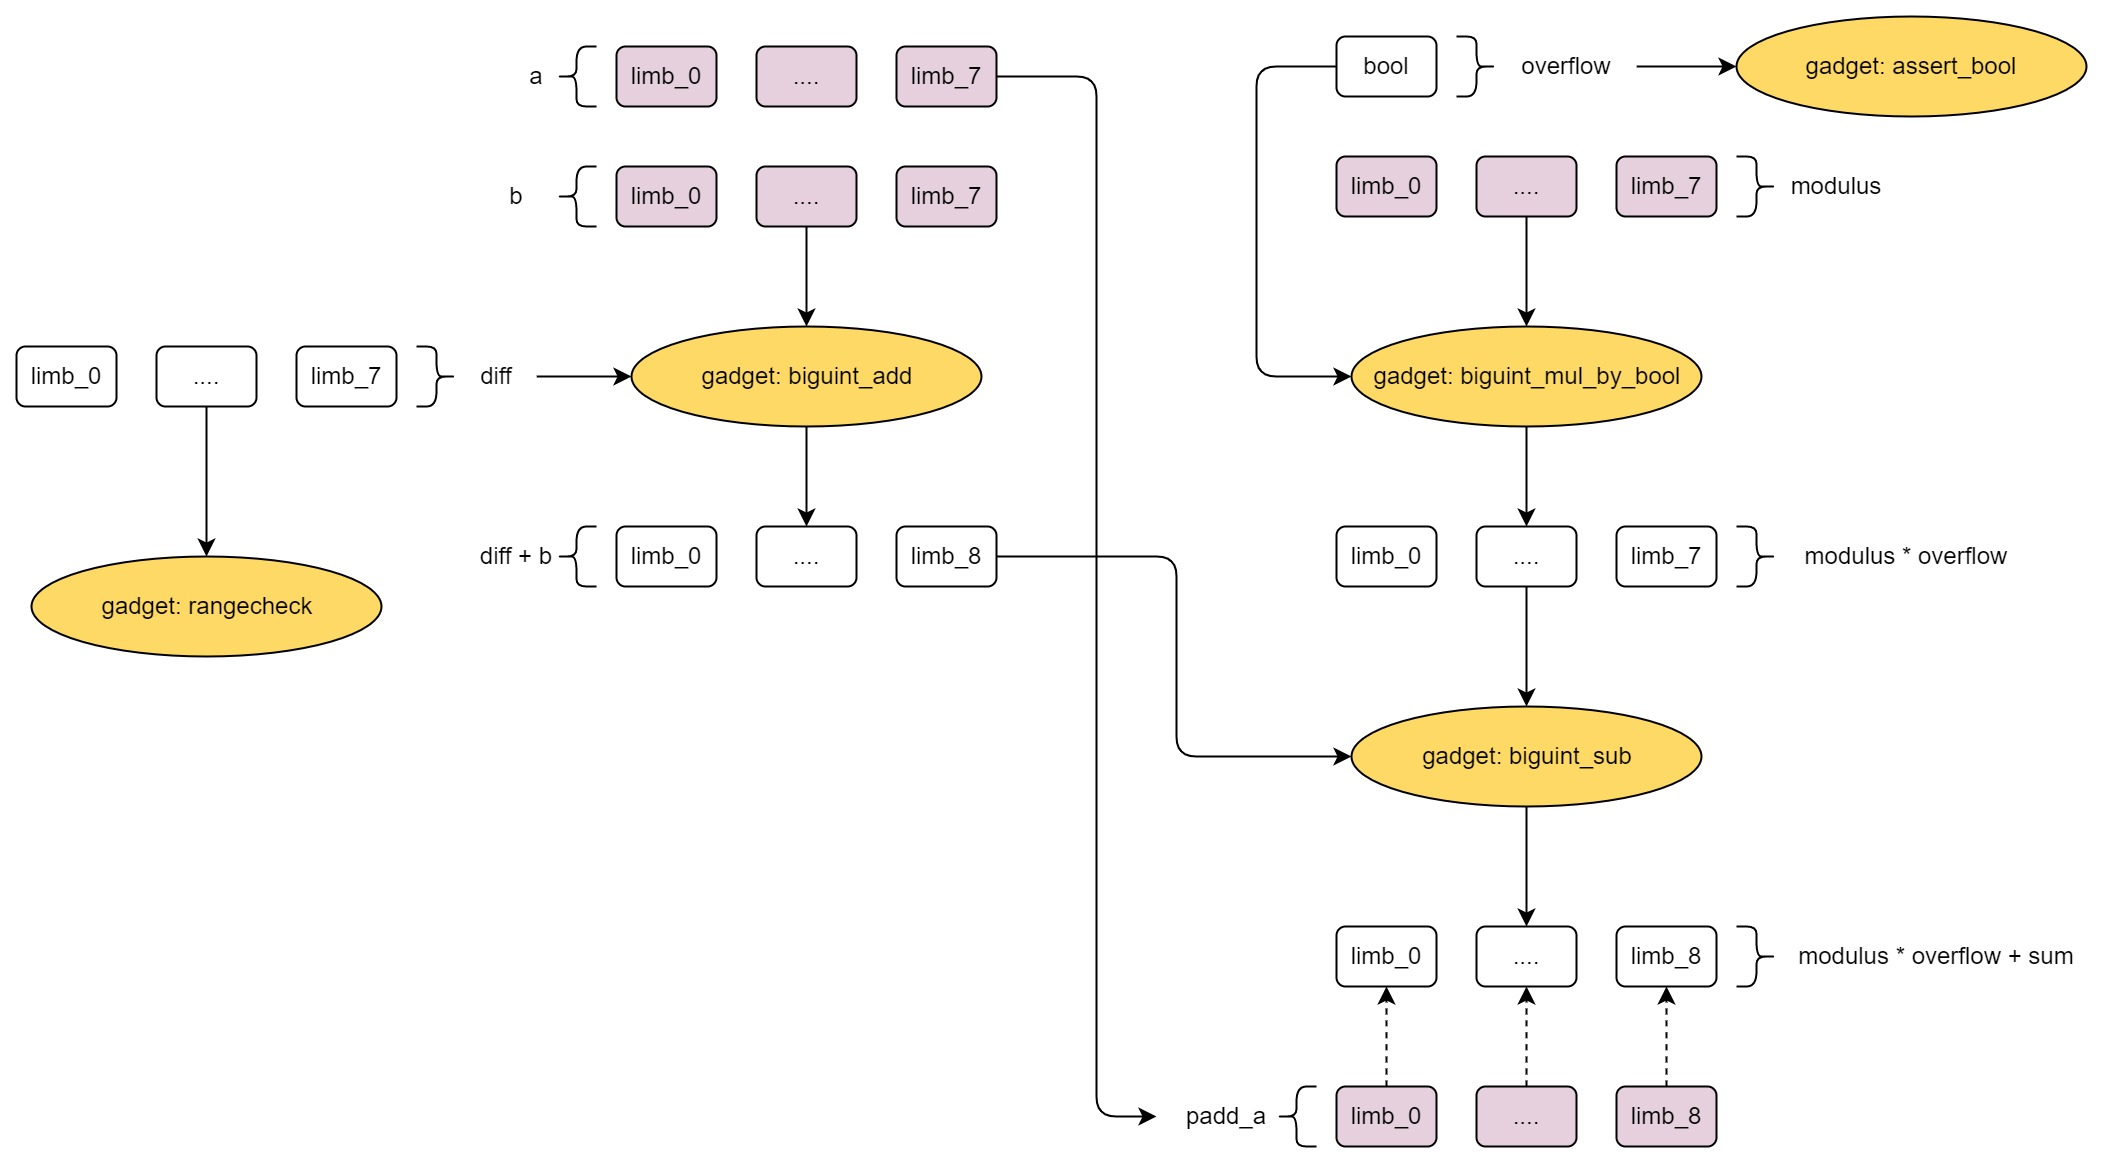
\includegraphics[width=0.8\textwidth]{nonnative-sub-layout.jpg}
            \caption{nonnative-sub layout}
            \label{fig:nonnative-sub-layout}
        \end{figure}
    
    \item constraints-info and costs
        \begin{itemize}
            \item gadget biguint-add num: 1
            \item gadget biguint-sub num: 1
            \item gadget biguint-mul-by-bool num: 1
            \item gadget u32rangecheck num: 1
            \item gadget assert-bool num: 1
            \item gate type num: 4(U32AddManyGate, U32SubtractionGate, U32RangeCheckGate, ArithmeticGate)
            \item gate instance num: 7 = 2(U32AddManyGate) + 2(U32SubtractionGate) + 1(U32RangeCheckGate) + 1(ArithmeticGate(1,0)) + 1(ArithmeticGate(1,-1))
            \item copy-constraints: 89 = 32{biguint-add num} + 27{U32SubtractionGate} + 9{biguint-mul-by-bool} + 8{u32rangecheck} + 4{assert-bool} + 9
        \end{itemize}

    \item questions
        \begin{itemize}
            \item why not constraint for overflow at nonnative-add?
            \item why not make u32rangecheck for input at nonnative-add?
        \end{itemize}

\end{enumerate}
    \subsubsection{nonnative-mul}
\label{nonnative-mul}

\begin{enumerate}
    \item target
        check the multiplicatipn relation among three nonnative target objects.
    \item constraints-logic
        \begin{itemize}
            \item check equation for gadget,  a * b = prod + modular * overflow
            \item check that "overflow.limb is U32"
            \item check that "prod.limb is U32"
        \end{itemize}
    \item nonnative-mul process layout
        \begin{figure}[!ht]
            \centering
            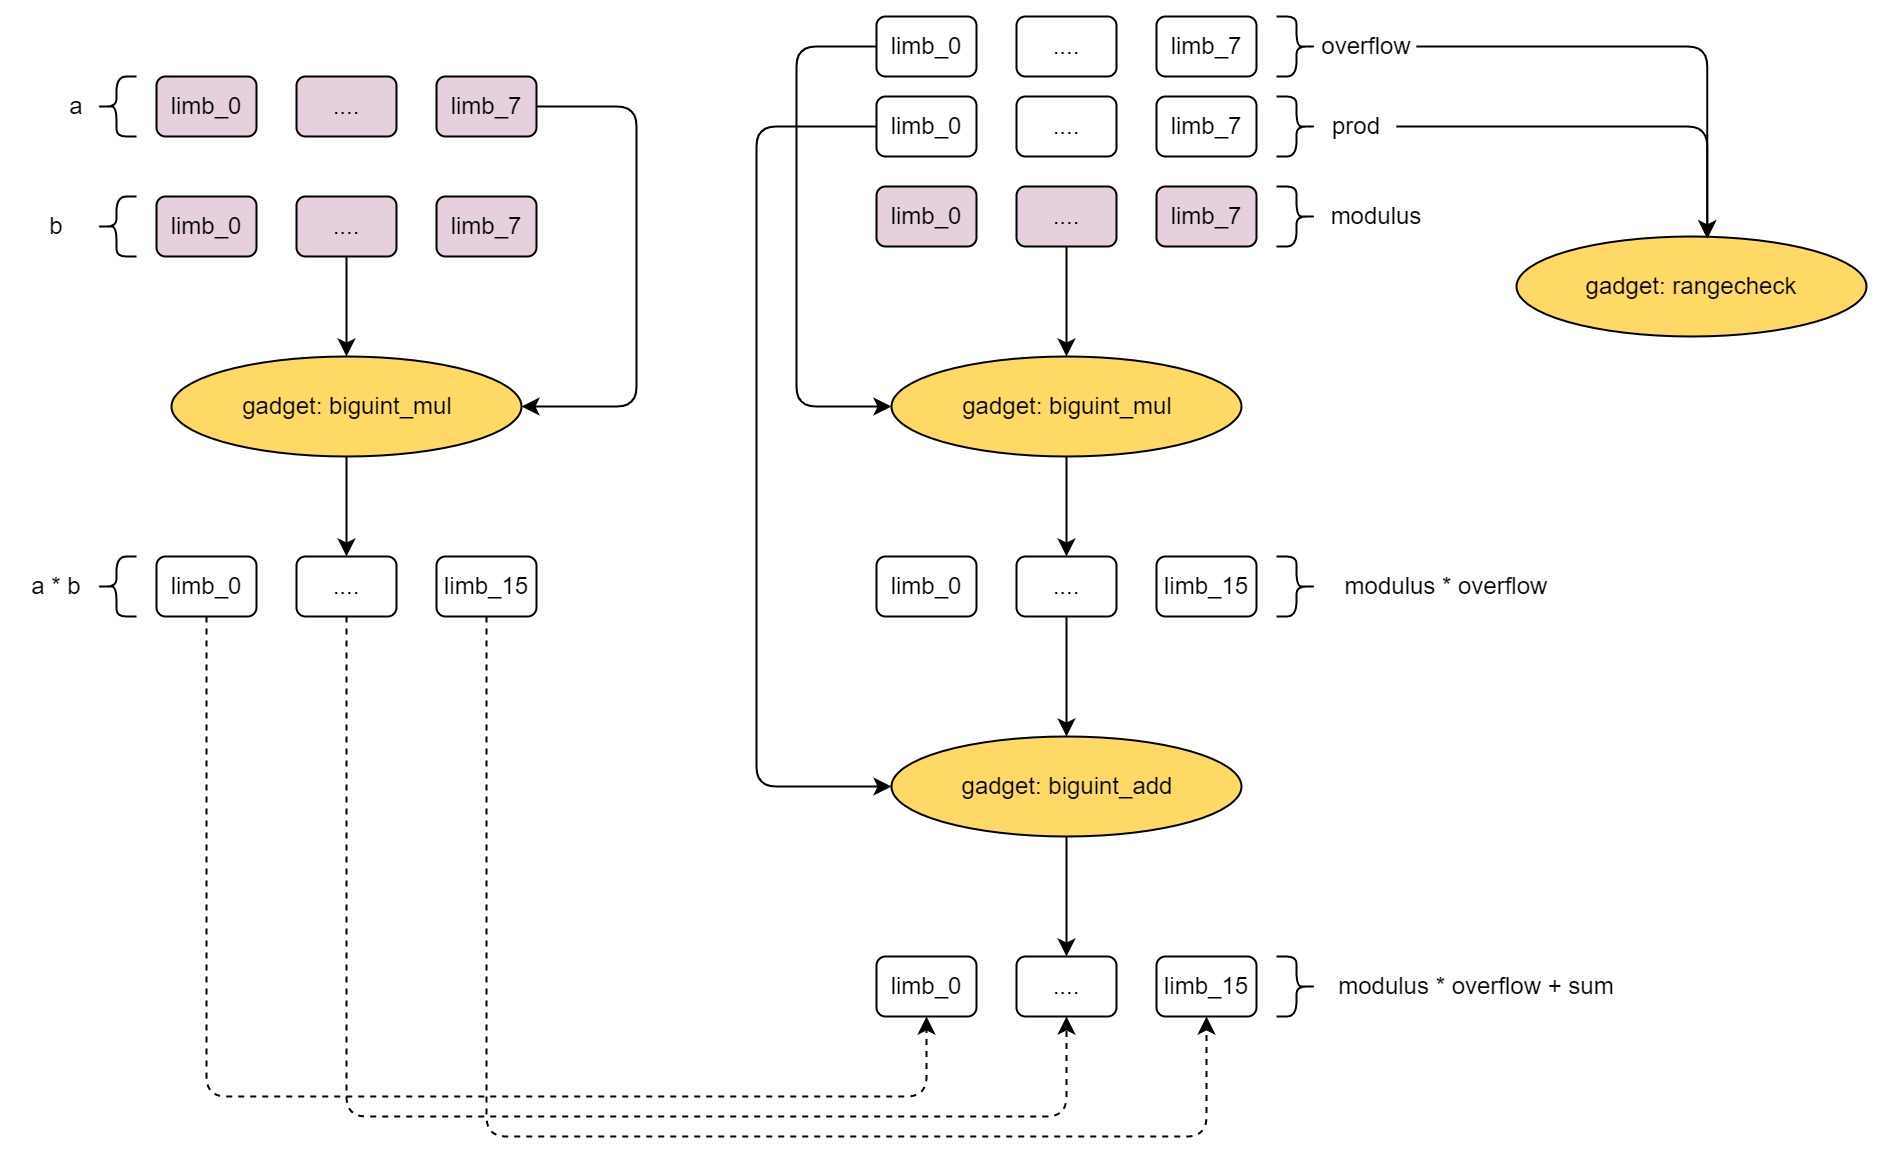
\includegraphics[width=0.8\textwidth]{nonnative-mul-layout.jpg}
            \caption{nonnative-mul layout}
            \label{fig:nonnative-mul-layout}
        \end{figure}
    
    \item constraints-info and costs
        \begin{itemize}
            \item gadget biguint-add num: 1
            \item gadget biguint-mul num: 2
            \item gadget u32rangecheck num: 2
            \item gate type num: 9 = 7(U32AddManyGate{3,5,7,9,11,13,15}) + 1(U32RangeCheckGate) + 1(U32ArithmeticGate)
            \item gate instance num: 37 = 2(u32rangecheck) + 8(biguint-mul: constant-input) + 22(biguint-mul) + 1 + 3(biguint-add)
            \item copy-constraints: 583 = 8 * 2(u32rangecheck) + 3 * 3 + (4 + 6 + 8 + 10 + 12 + 14 + 16) * 4 + (8 * 8) * 3 + 17 * 4 + 18
        \end{itemize}

\end{enumerate}
    \subsubsection{nonnative-inv}

\Par{Target}
Check the modular inverse relation among three nonnative target objects.

\Par{Constraints logic}
\begin{itemize}
    \item Check equation for gadget: \verb|a * inv_a = 1 + modular * div|.
\end{itemize}

\Par{Process layout}
See \figref{fig:nonnative-inv-layout}.
\begin{figure}[!ht]
    \centering
    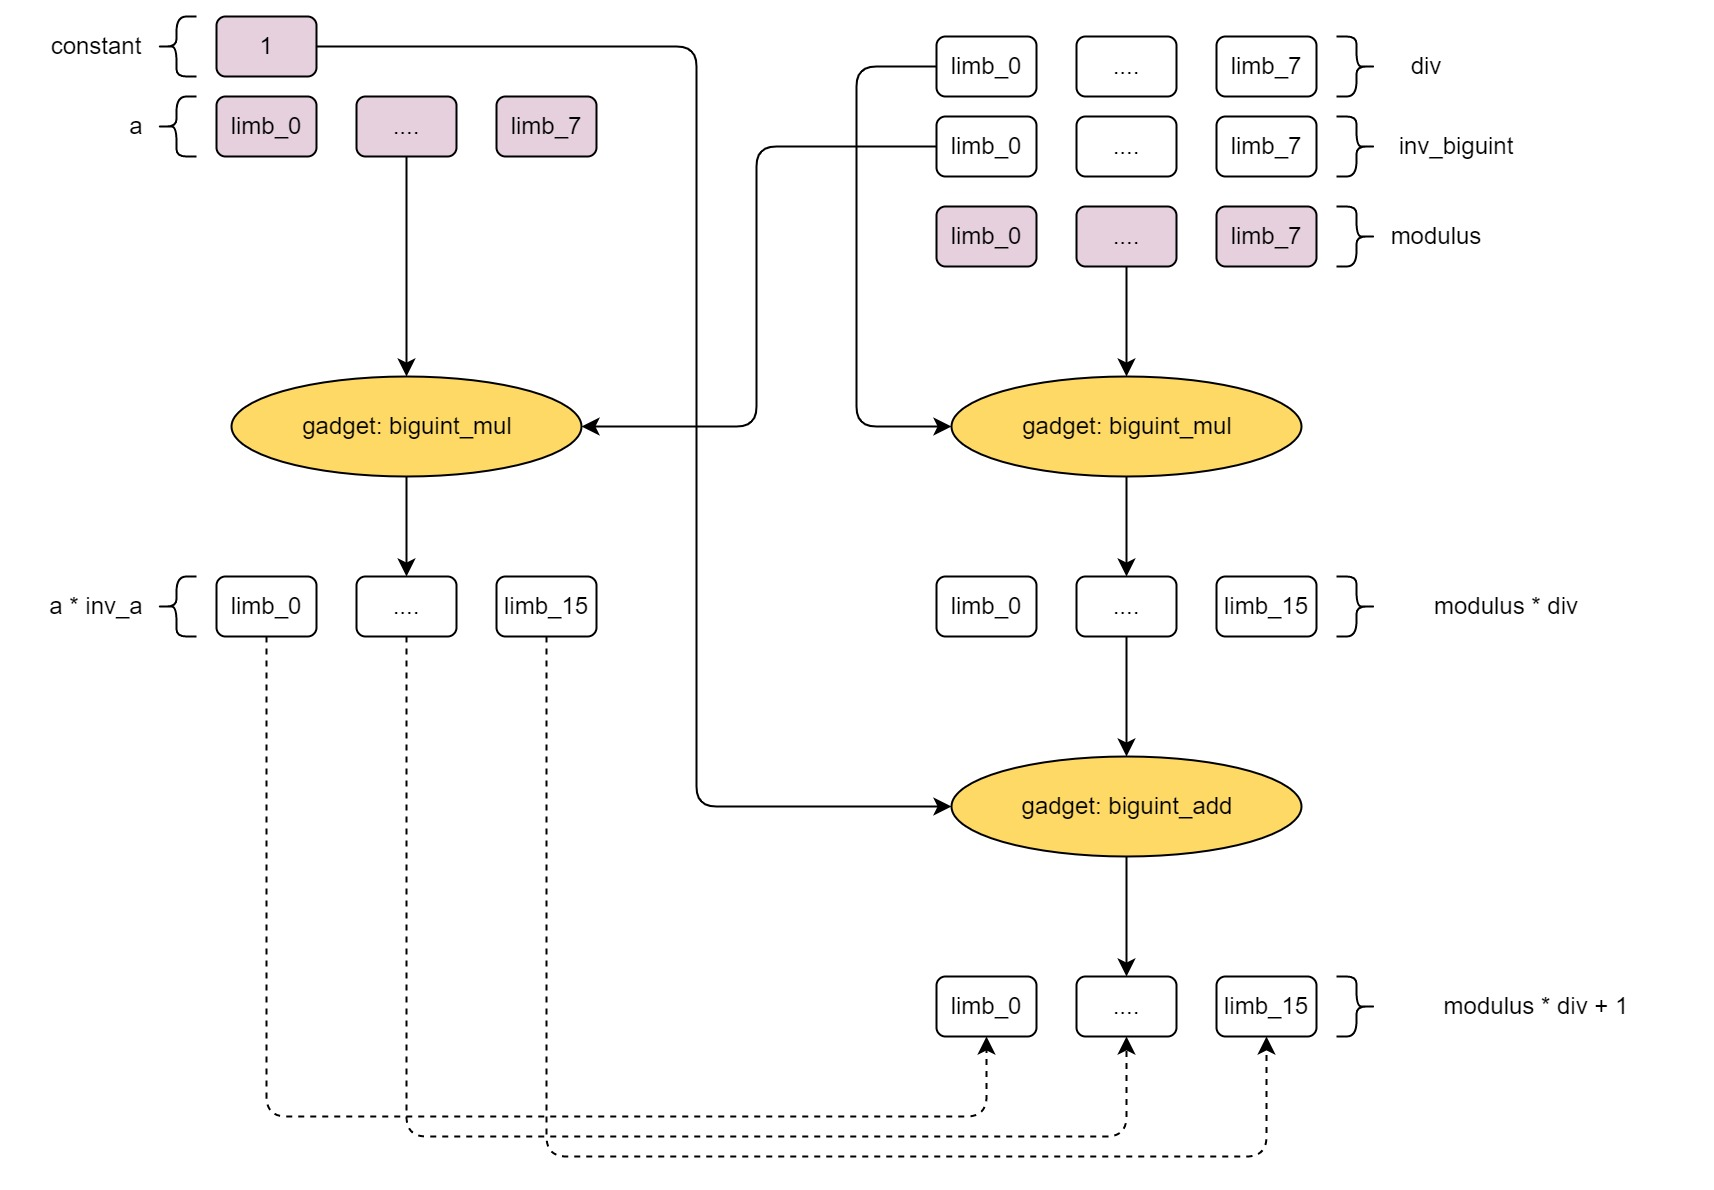
\includegraphics[width=0.8\textwidth]{nonnative-inv-layout.jpg}
    \caption{nonnative-inv layout}
    \label{fig:nonnative-inv-layout}
\end{figure}

\Par{Constraints info and costs}
\begin{itemize}
    \item gadget biguint-add num: 1
    \item gadget biguint-mul num: 2
    \item gate type num: 8 = 7(U32AddManyGate\{3,5,7,9,11,13,15\}) + 1(U32ArithmeticGate)
    \item gate instance num: 56 = (8 * 8 + 2) * 2 / 3 + 5(U32AddManyGate{3}) + 5 + 2(U32AddManyGate{15})
    \item copy-constraints: 762 = (8 * 8 + 2) * 2 * 3 + 21 * 4 + (6 + 8 + 10 + 12 + 14) * 4 + 4 * 16 + 18
\end{itemize}

    \section{curve-add}
\label{curve-add}

Take curve-secp256k1 as example, the same as other texs.

\begin{enumerate}
    \item target
        implement the addition of two different curve points. this is a incomplete addition, you can refer to The halo2 Book \cite{website:halo2-book} to learn more about it.
    \item constraints-logic
        \begin{figure}[!ht]
            \centering
            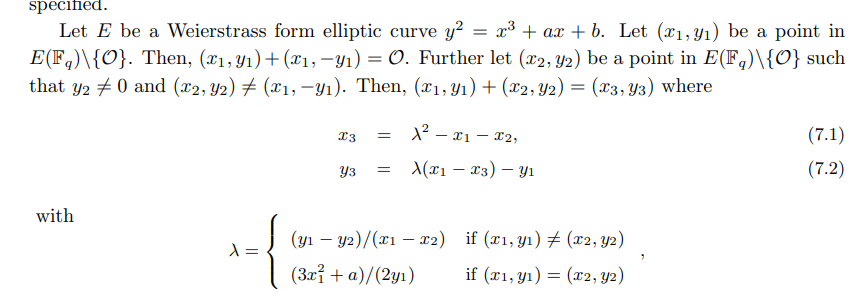
\includegraphics[width=0.8\textwidth]{curve-add.jpg}
            \caption{curve-add}
            \label{fig:curve-add}
        \end{figure}
    \item curve-add process layout
        \begin{figure}[!ht]
            \centering
            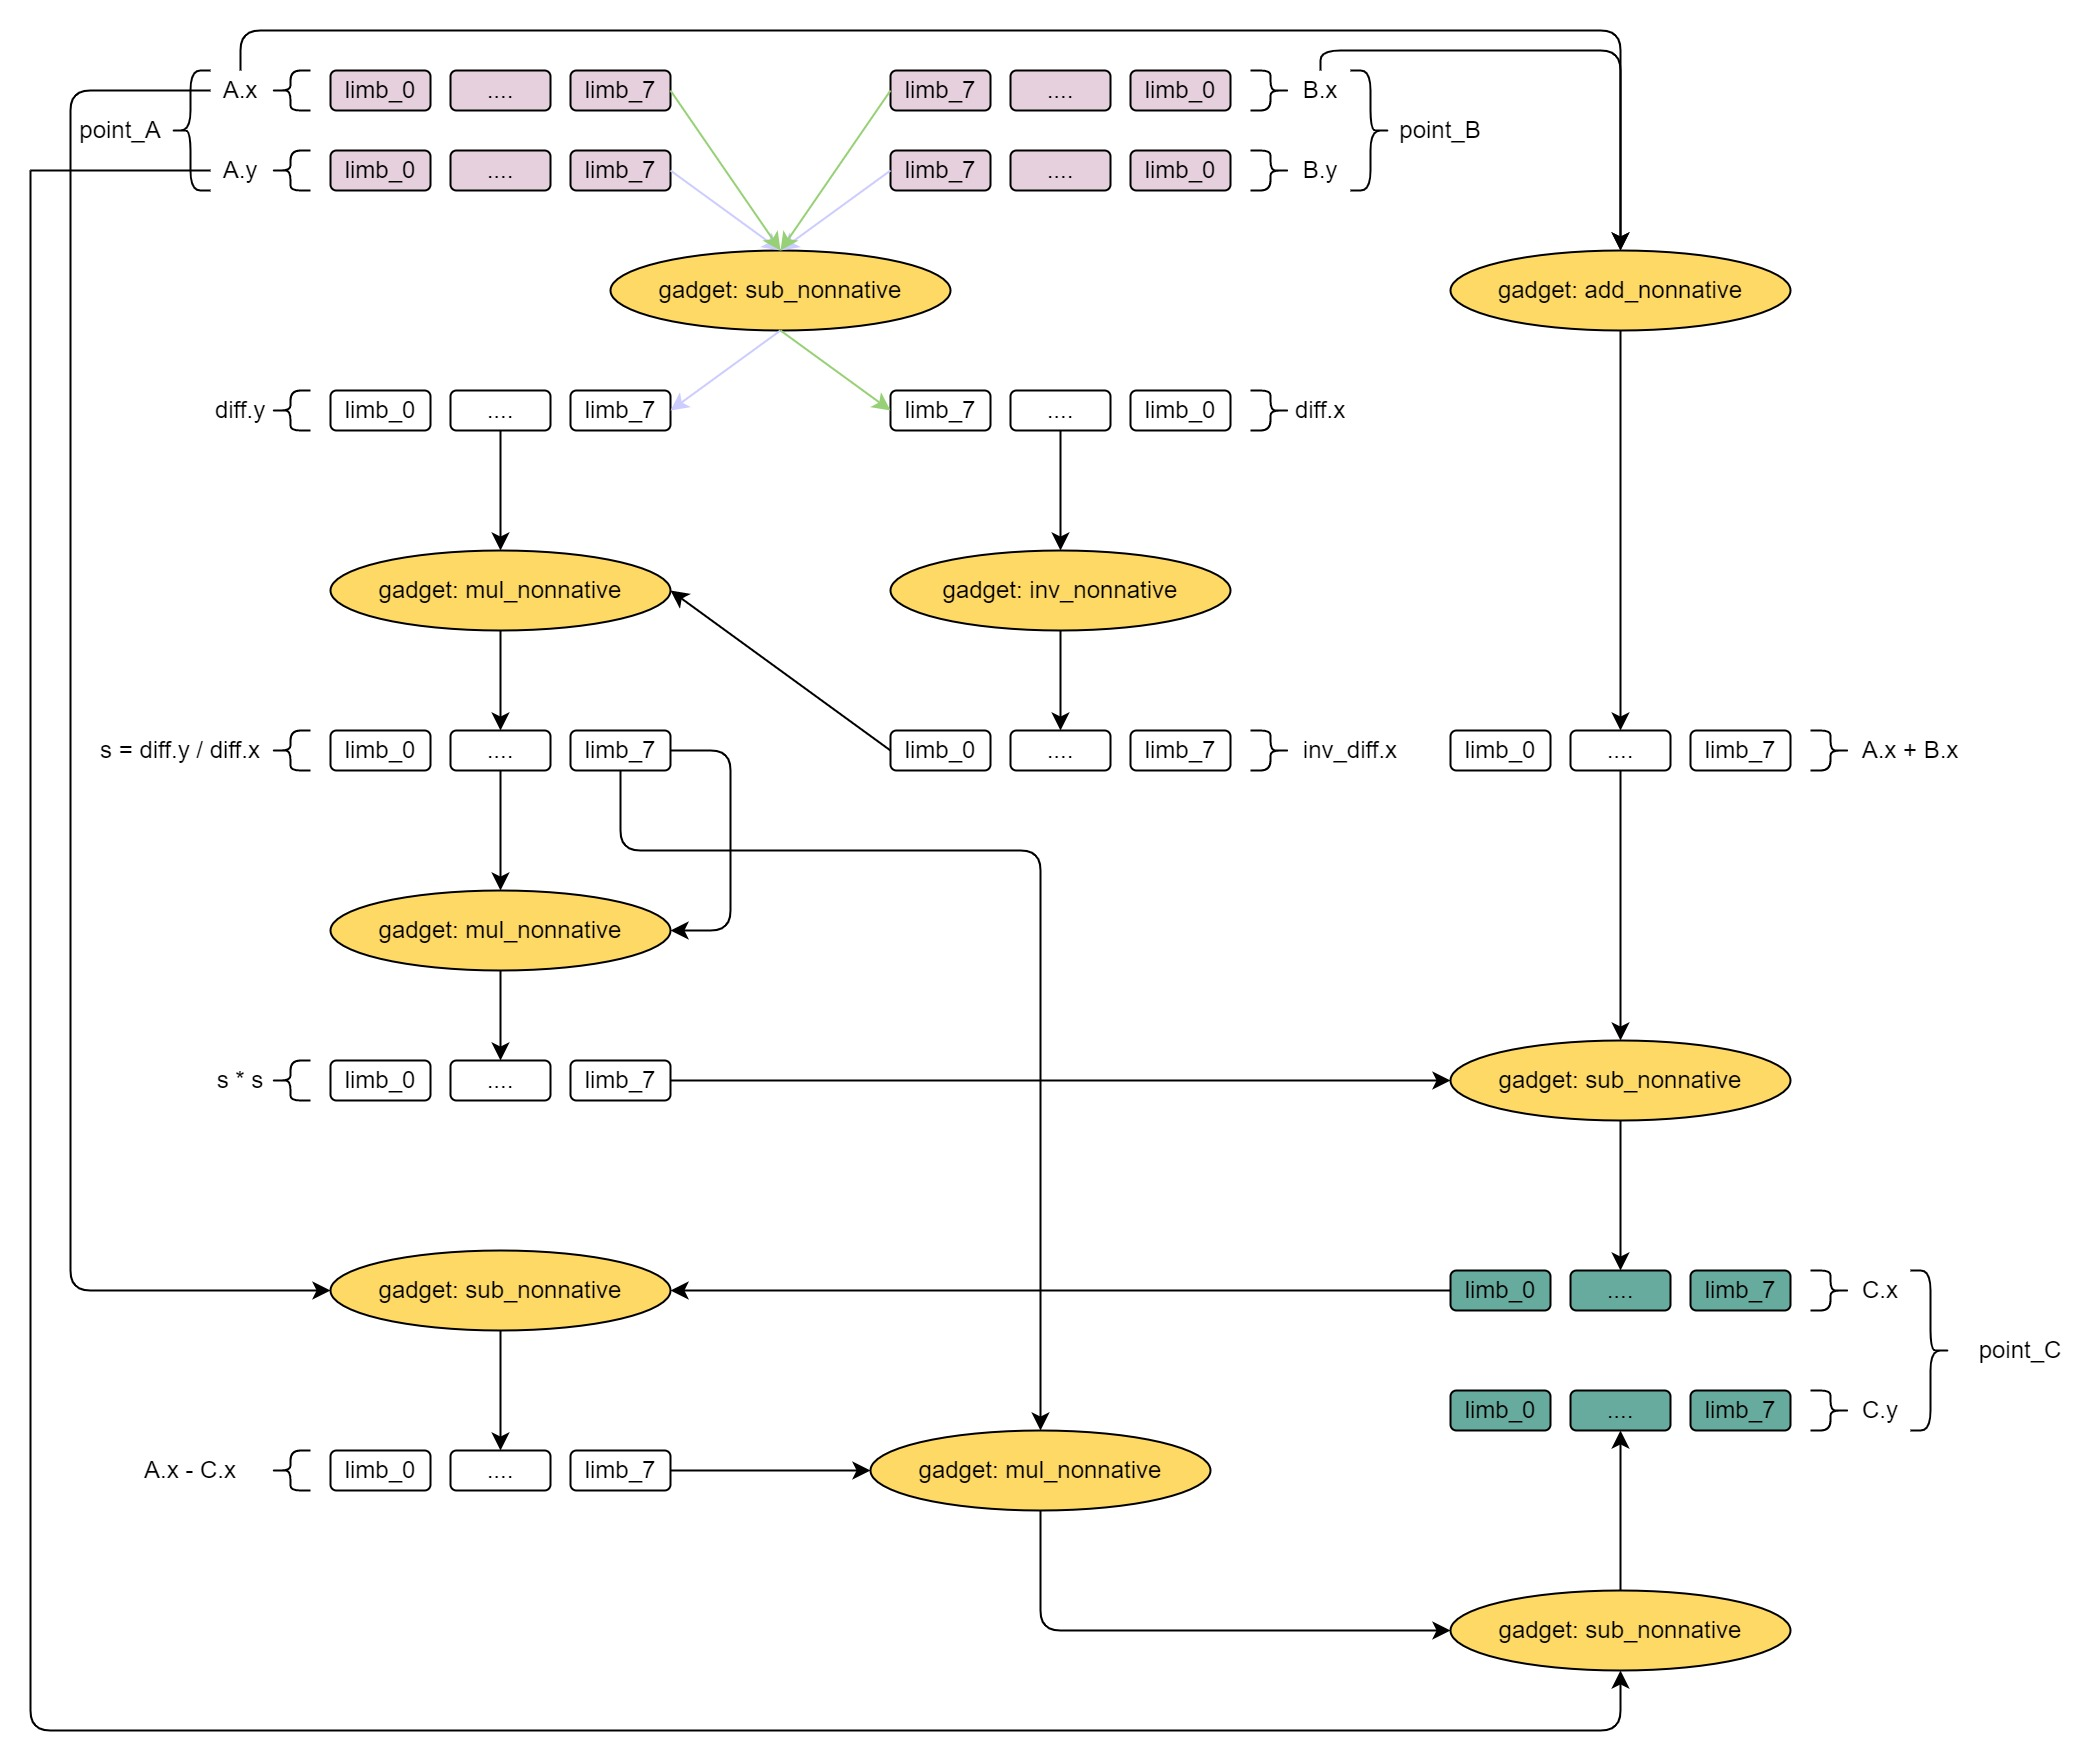
\includegraphics[width=0.8\textwidth]{curve-add-layout.jpg}
            \caption{curve-add layout}
            \label{fig:curve-add-layout}
        \end{figure}
    
    \item constraints-info and costs
        \begin{itemize}
            \item gadget-sub-nonnative num: 5
            \item gadget-add-nonnative num: 1
            \item gadget-mul-nonnative num: 3
            \item gadget-inv-nonnative num: 1
            \item gate type num: 
            \item gate instance num: 
        \end{itemize}

\end{enumerate}
    %\printbibliography[heading=bibintoc, title=\ebibname]%
\end{document}

    \subsubsection{biguint-add}

\Par{Target}
Implement the addition of two biguints.

\Par{Constraints logic}
\begin{itemize}
    \item Equation for gates;
    \item Sumcheck between output and limbs;
    \item Rangecheck for limbs.
\end{itemize}

\Par{Circuit layout}
See \figref{fig:biguint-add-circuit-layout}.
\begin{figure}[!ht]
    \centering
    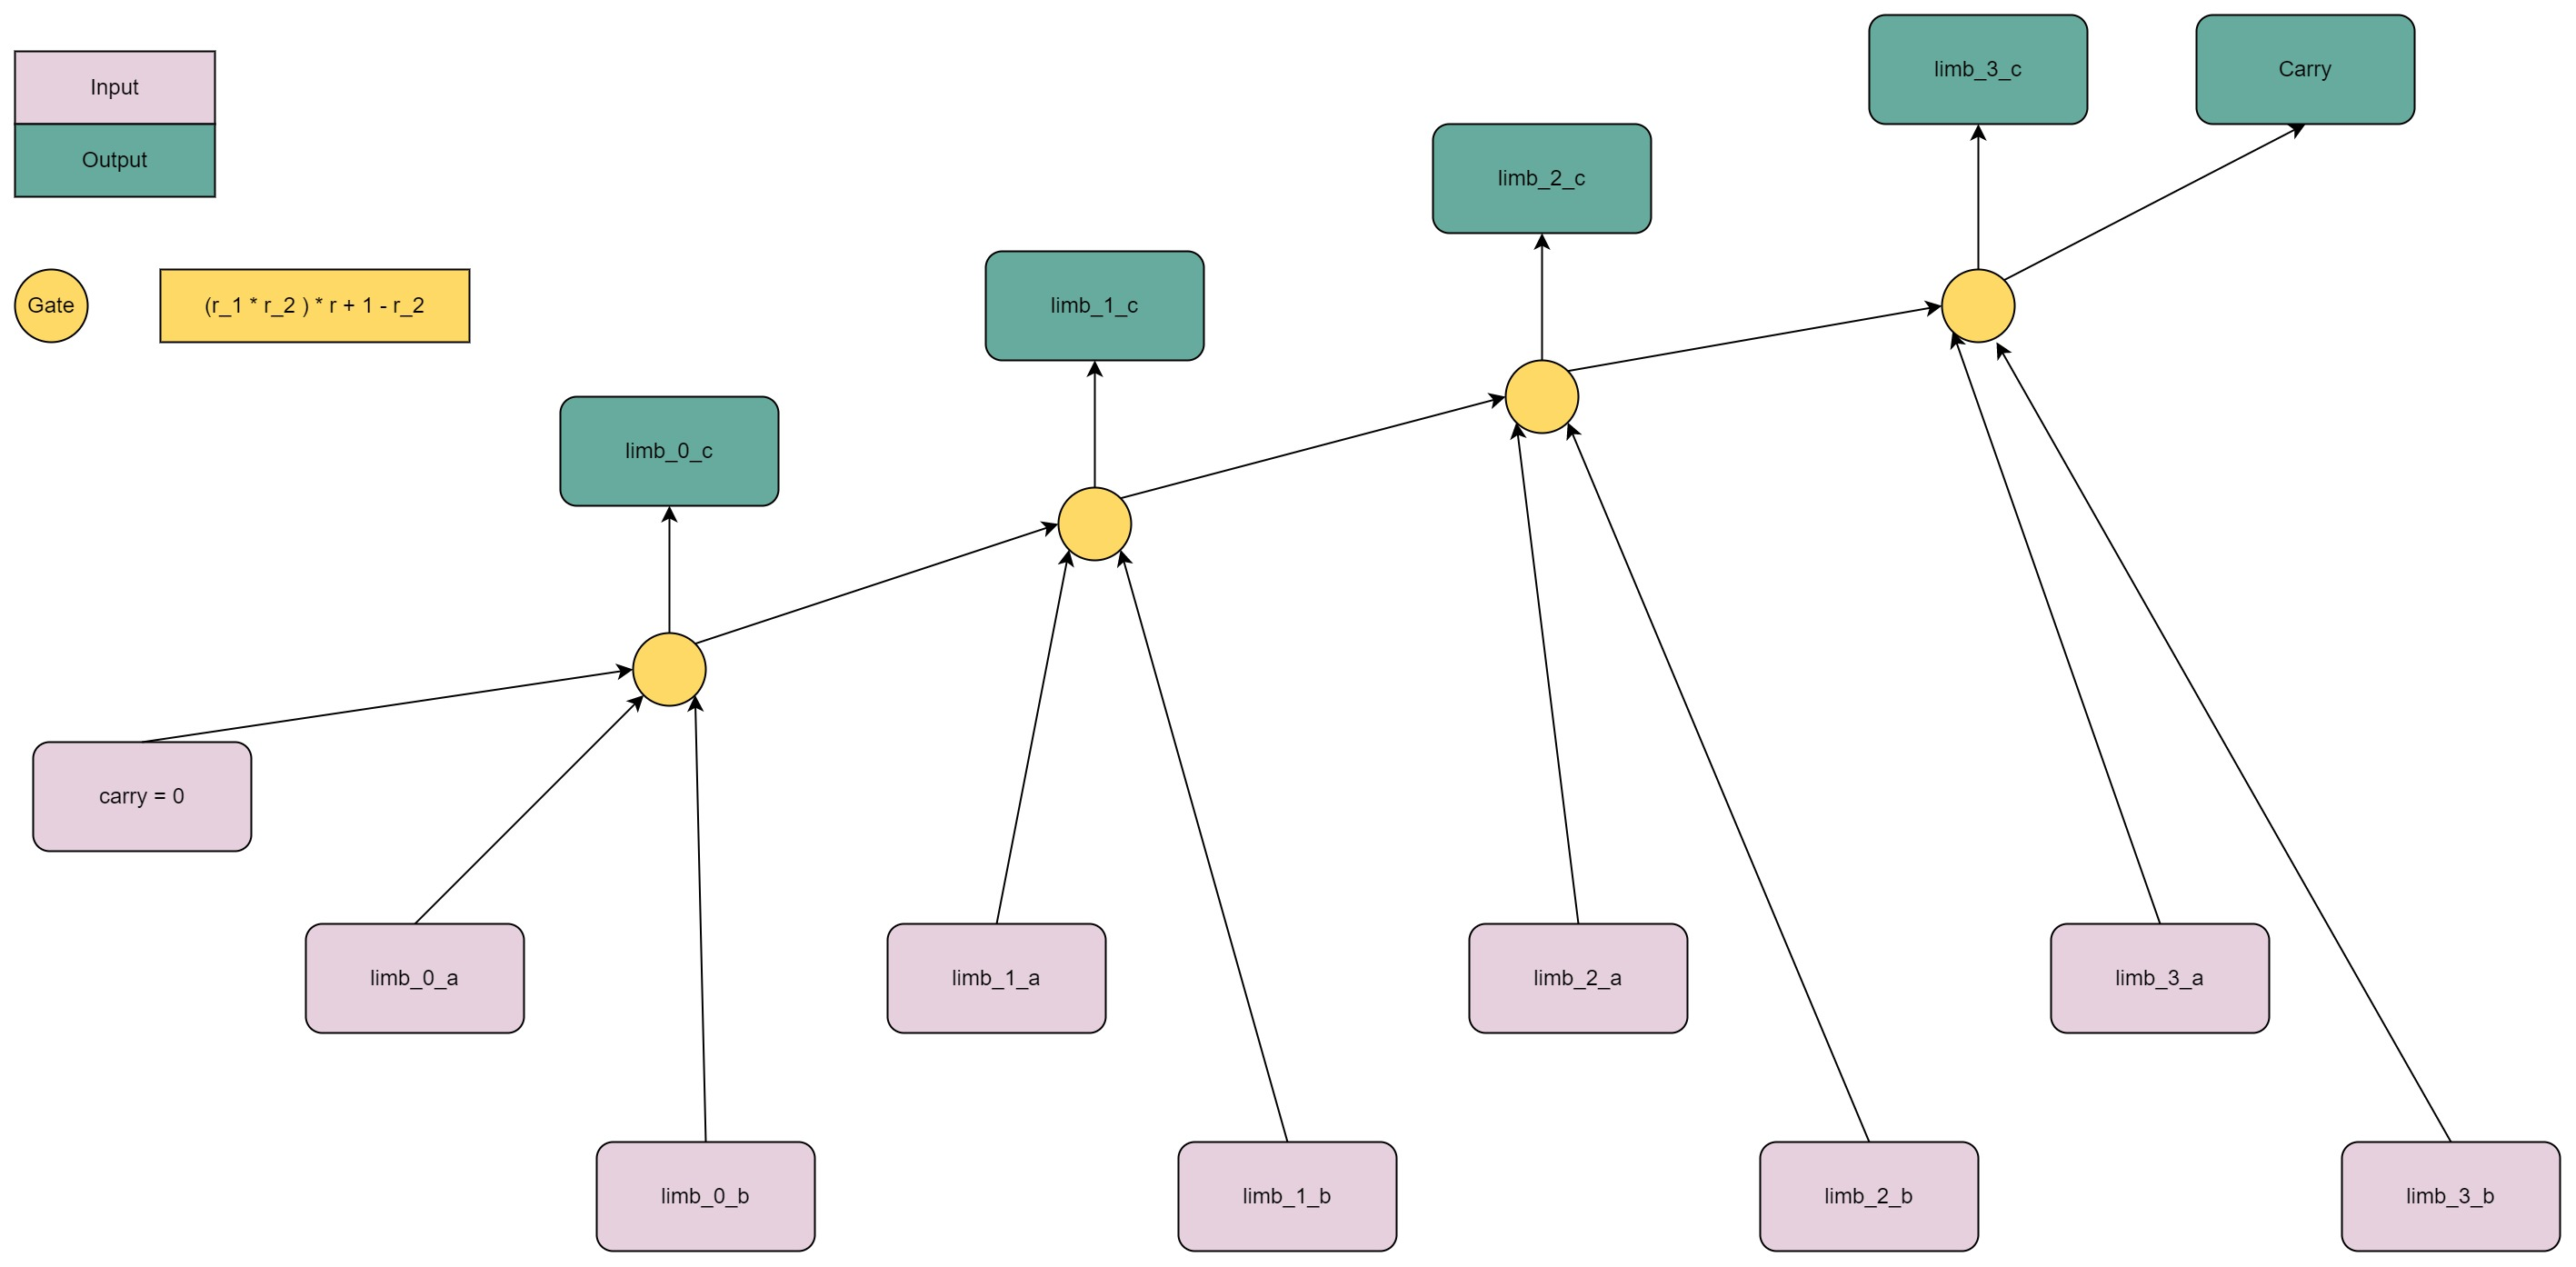
\includegraphics[width=0.8\textwidth]{biguint-add-circuit-layout.jpg}
    \caption{biguint-add circuit layout}
    \label{fig:biguint-add-circuit-layout}
\end{figure}

\Par{Trace layout}
See \figref{fig:biguint-add-trace-layout}.
\begin{figure}[!ht]
    \centering
    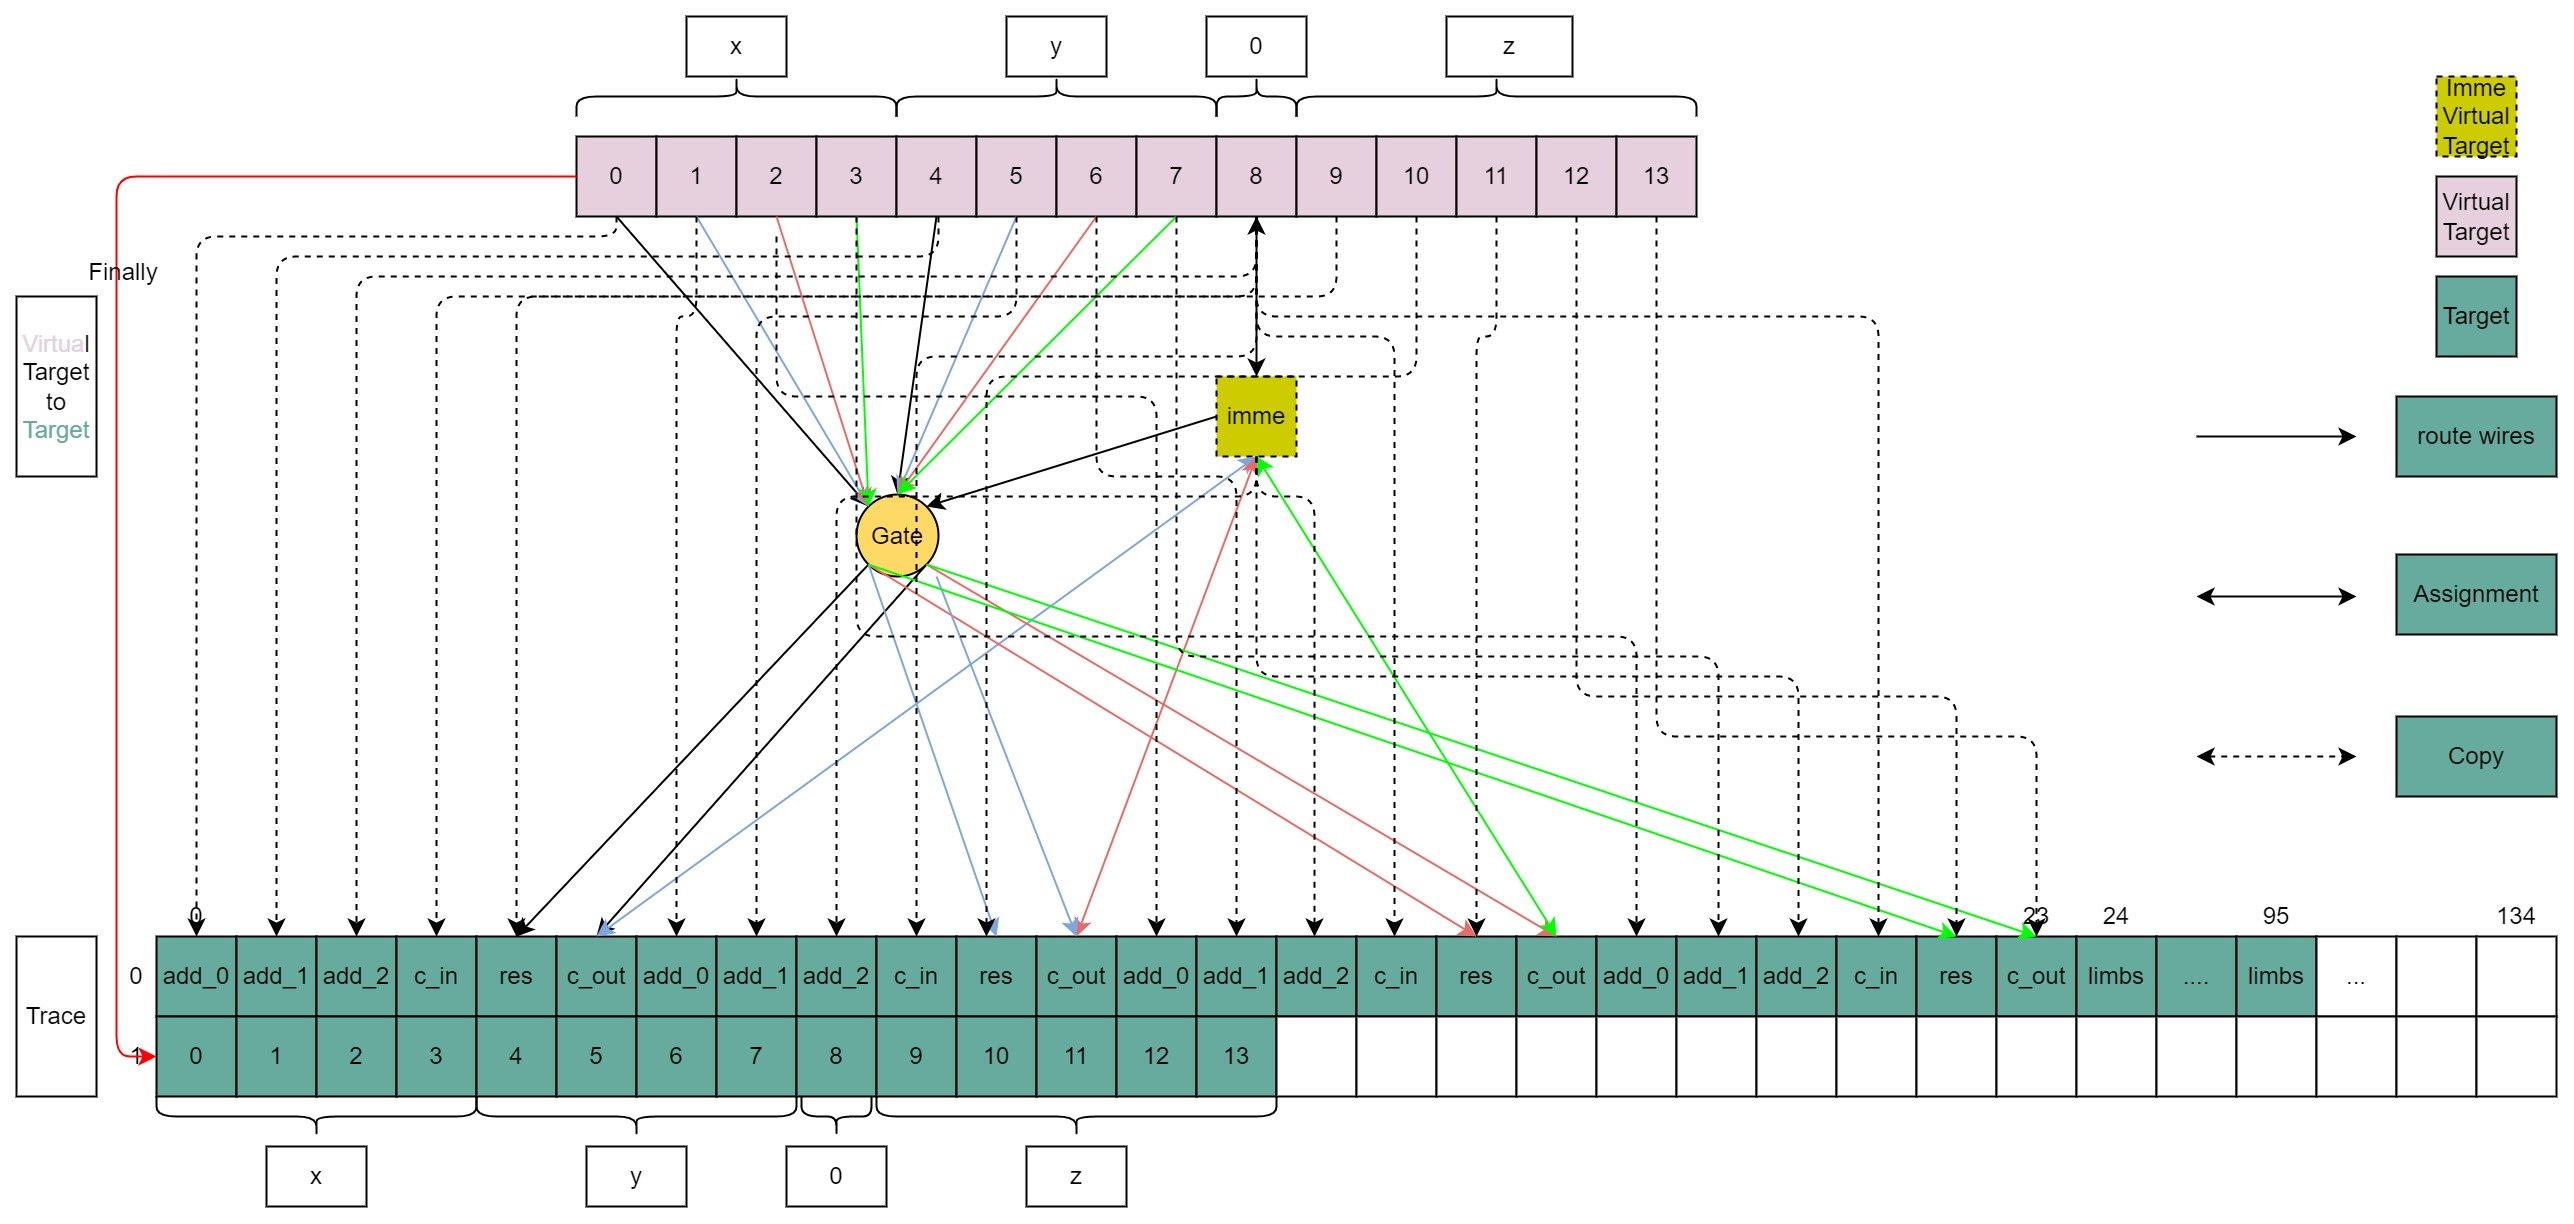
\includegraphics[width=0.8\textwidth]{biguint-add-trace-layout.jpg}
    \caption{biguint-add trace layout}
    \label{fig:biguint-add-trace-layout}
\end{figure}

\Par{Constraints info and costs}
\begin{itemize}
    \item gate type num: 1 (U32AddManyGate)
    \item gate ops num: limbs-num
    \item gate instance num: ceil(limbs-num / gate.ops)
    \item copy-constraints: limbs-num * 4
    \item max-degree: 4 (\verb|1 << limb-bits|)
\end{itemize}

\Par{Questions}
\begin{itemize}
    \item Why not make rangecheck constraint for inputs?
    \item Why not make copy constraint between cur-c-in and last-c-out?
\end{itemize}

    \subsubsection{biguint-sub}

\Par{Target}
Implement the substraction of two biguints.

\Par{Constraints logic}
\begin{itemize}
    \item Equation for gate;
    \item Sumcheck for ouptput;
    \item Rangecheck for limbs.
\end{itemize}

\Par{Circuit layout}
See \figref{fig:biguint-sub-circuit-layout}.
\begin{figure}[!ht]
    \centering
    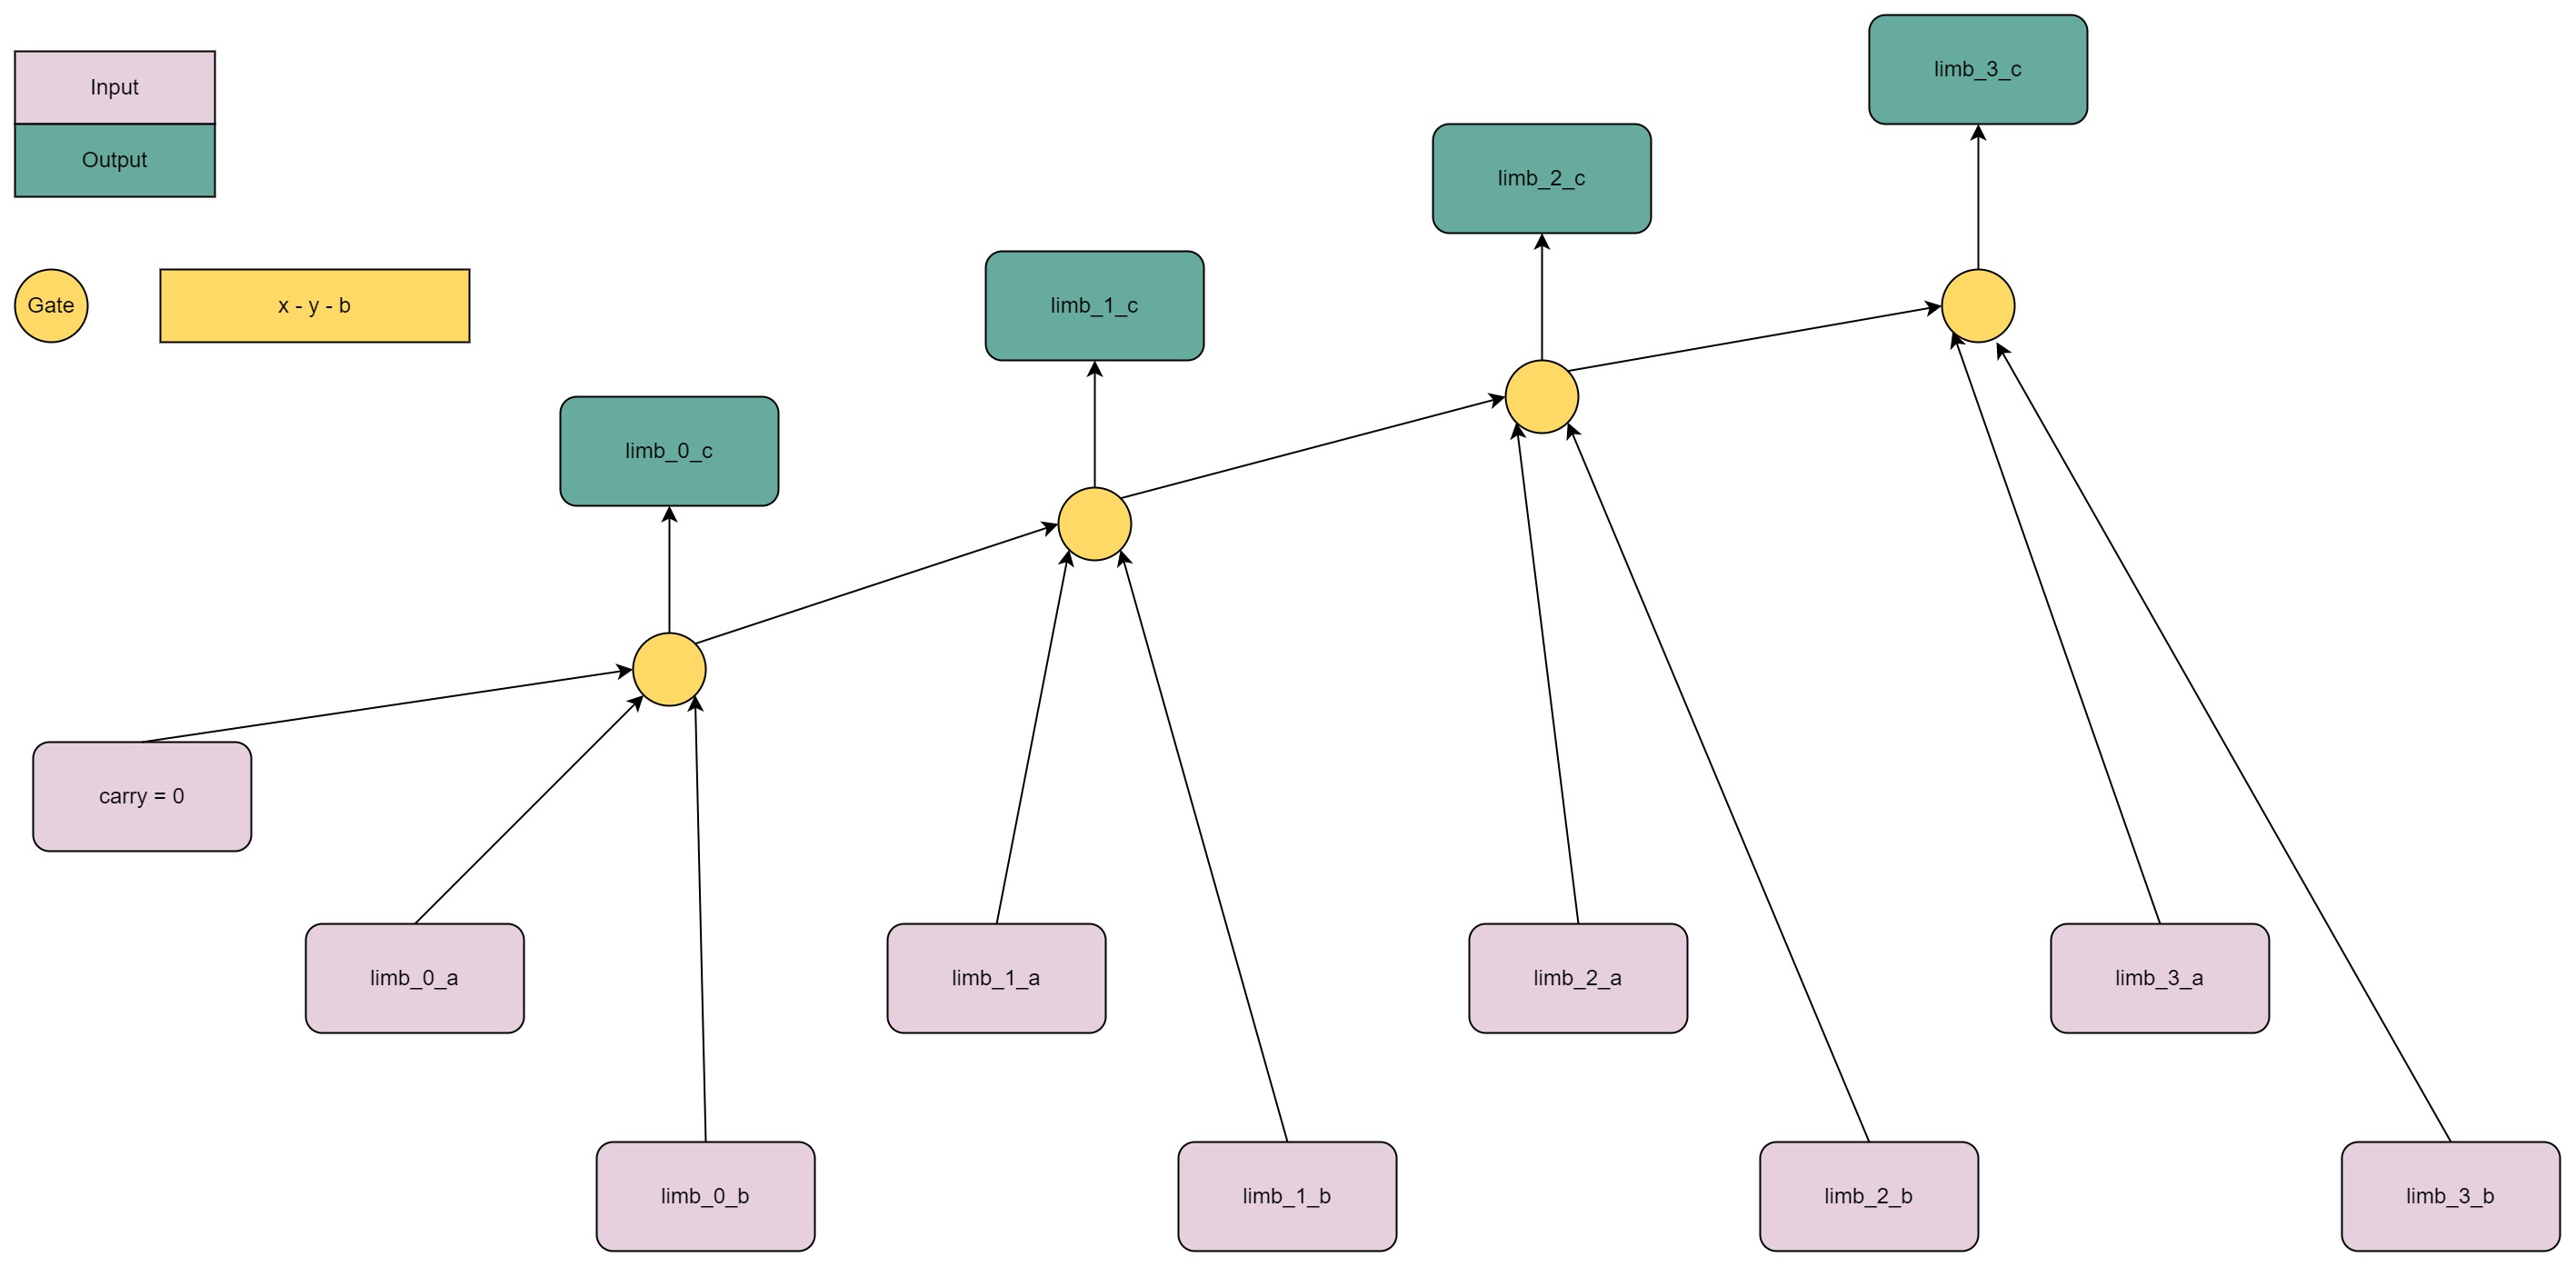
\includegraphics[width=0.8\textwidth]{biguint-sub-circuit-layout.jpg}
    \caption{biguint-sub circuit layout}
    \label{fig:biguint-sub-circuit-layout}
\end{figure}

\Par{Trace layout}
See \figref{fig:biguint-sub-trace-layout}.
\begin{figure}[!ht]
    \centering
    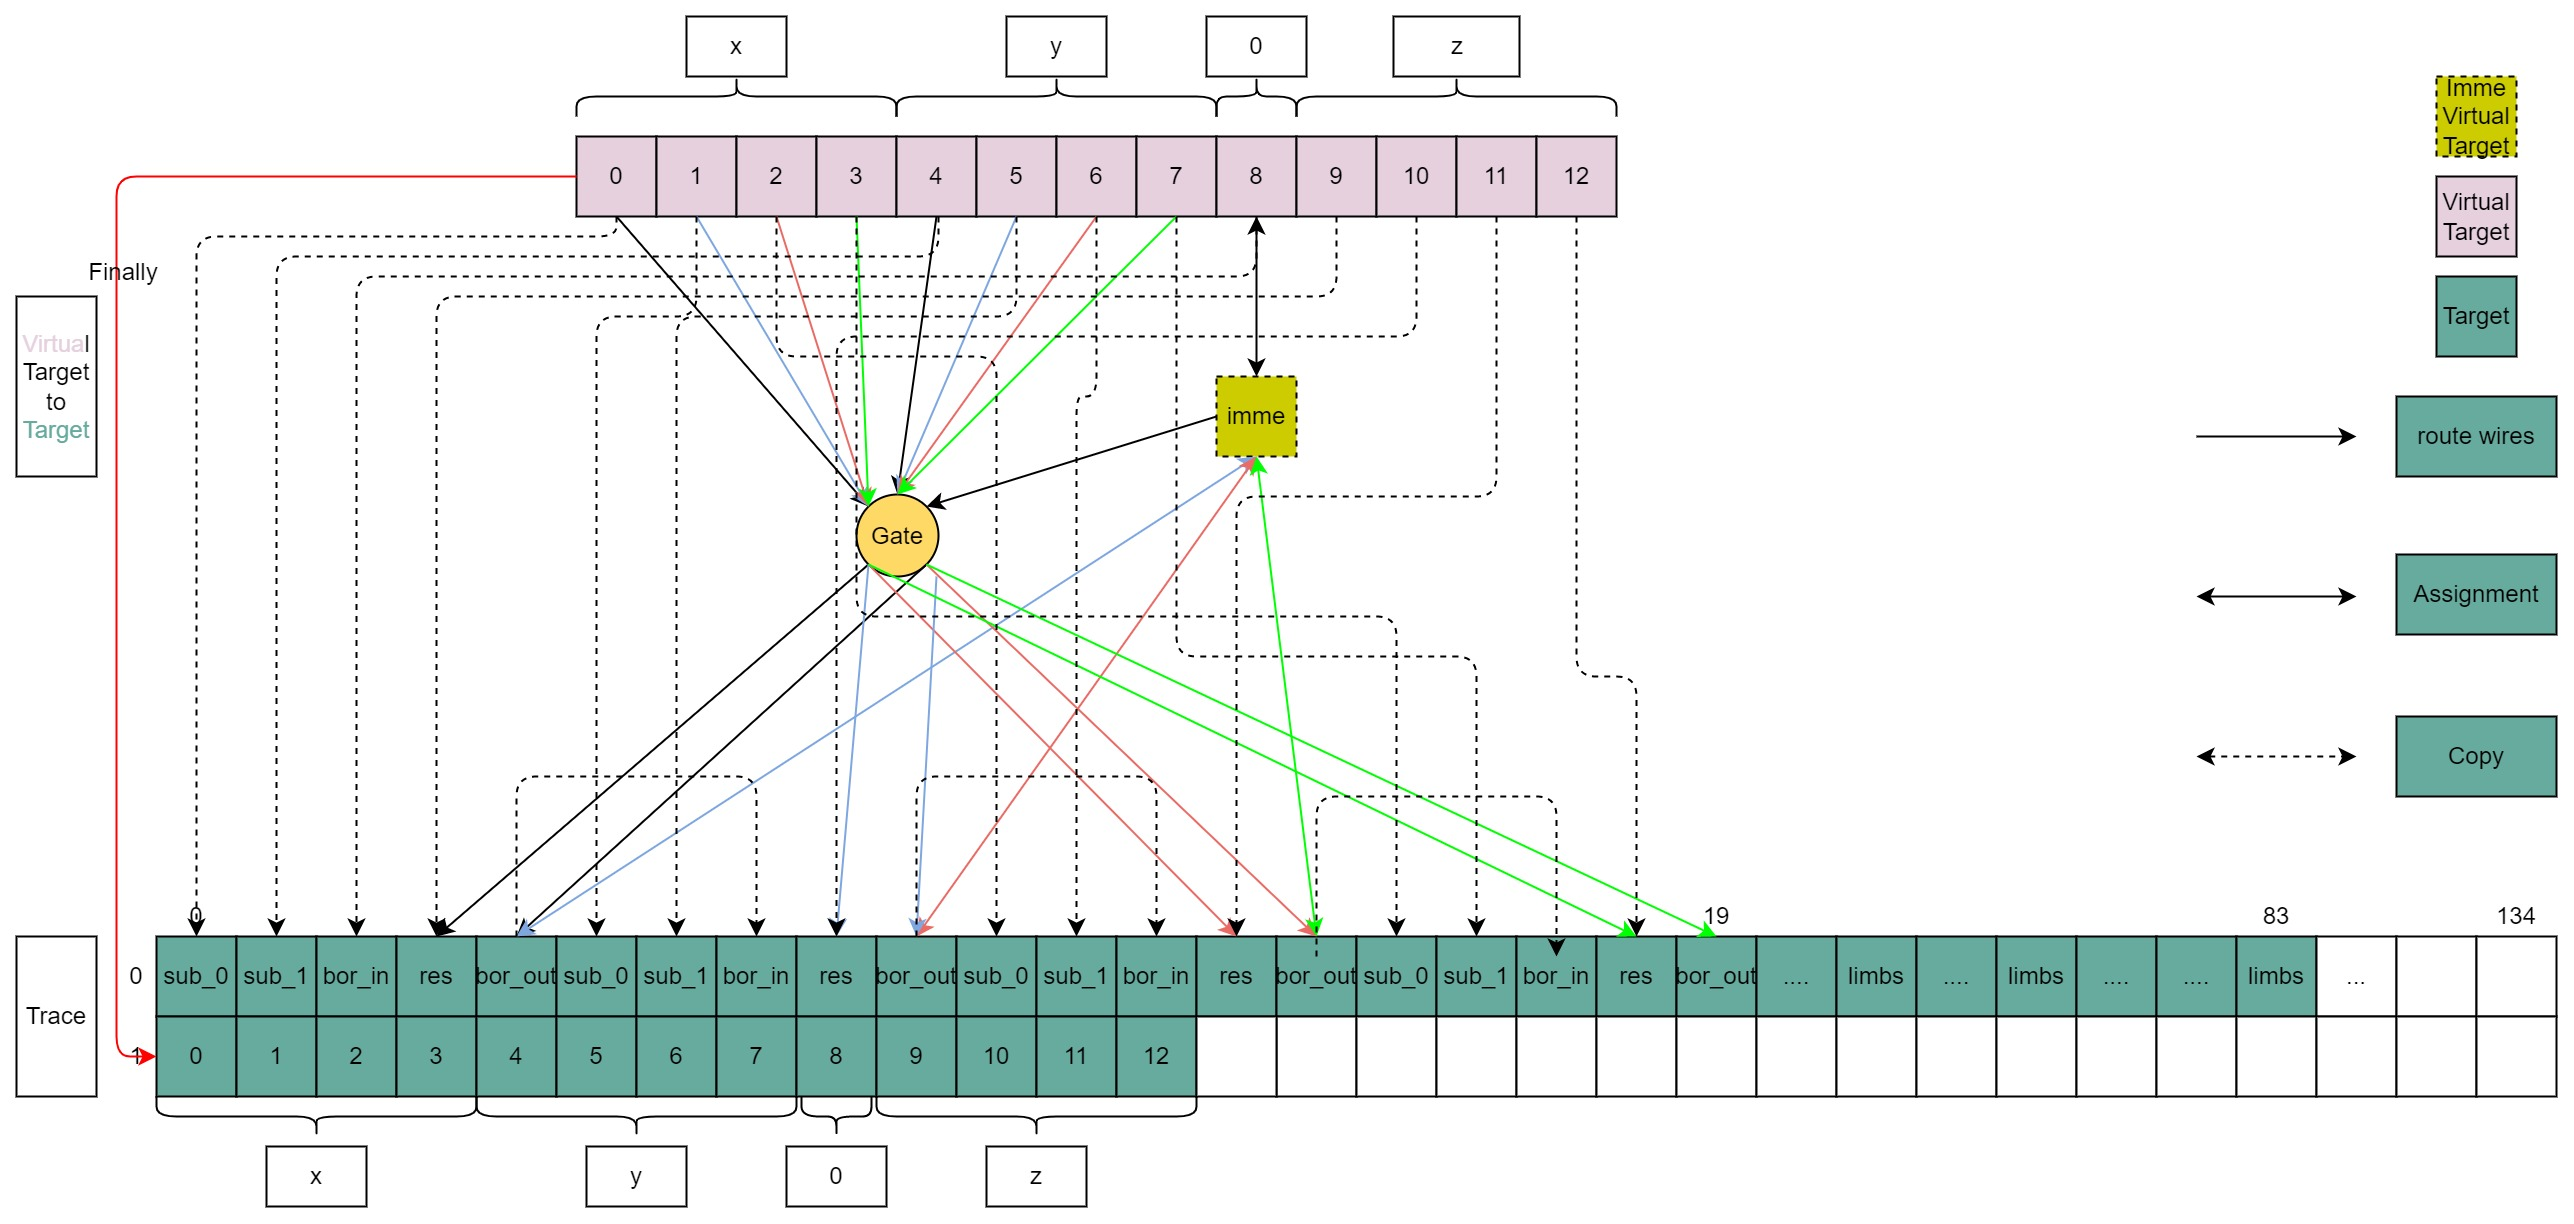
\includegraphics[width=0.8\textwidth]{biguint-sub-trace-layout.jpg}
    \caption{biguint-sub trace layout}
    \label{fig:biguint-sub-trace-layout}
\end{figure}

\Par{Constraints info and costs}
\begin{itemize}
    \item constraints-num: $6 \times (3 + 32 / 2) = 114$
    \item copy-constraints: $16$
    \item max-degree: $4$
    \item wires-num: $6 \times (5 + 16) = 126$
\end{itemize}

\Par{Questions}
\begin{itemize}
    \item Why not make rangecheck constraint for inputs?
    \item Could try to use the same constraint with add-gate.
\end{itemize}

    \subsubsection{biguint-mul}

\Par{Target}
Implement the multiplication of two biguints.

\Par{Constraints logic}
\begin{itemize}
    \item Compute mul-factors first, use U32ArithmeticGate;
    \item Add mul-factors from low bits, use U32AddManyGate.
\end{itemize}

\Par{Process layout}
See \figref{fig:biguint-mul-layout}
\begin{figure}[!ht]
    \centering
    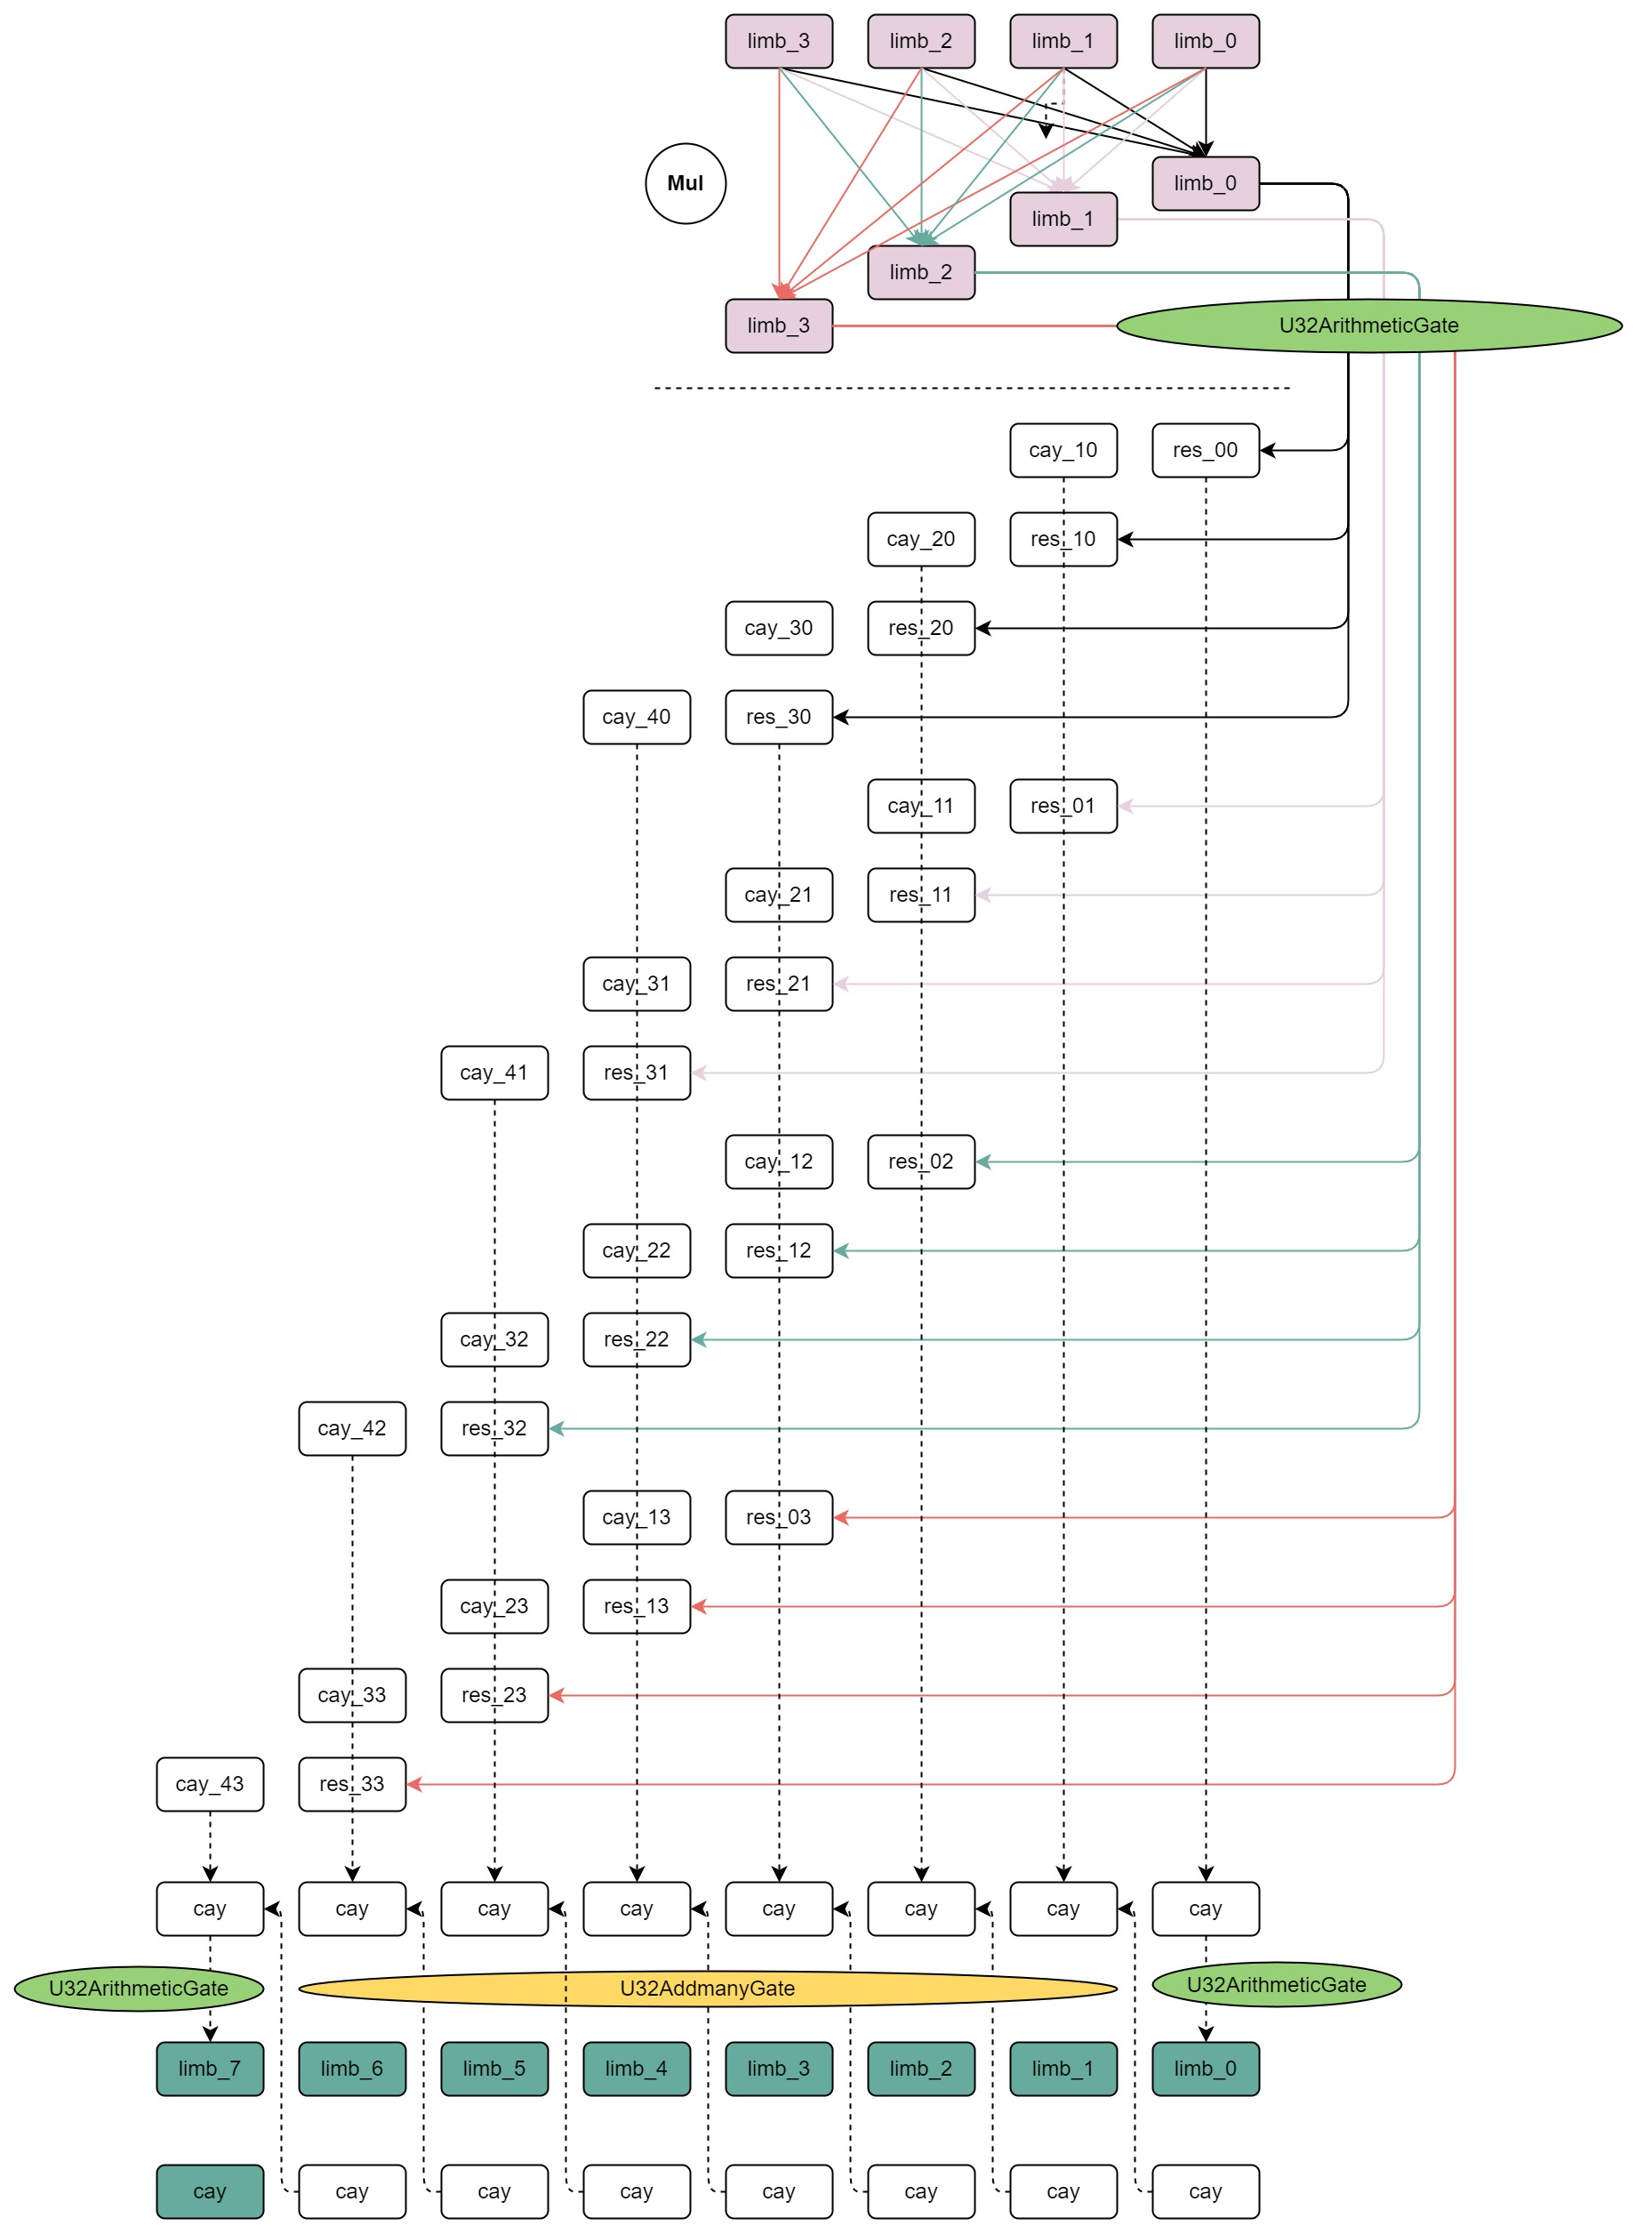
\includegraphics[width=0.8\textwidth]{biguint-mul-layout.jpg}
    \caption{biguint-mul layout}
    \label{fig:biguint-mul-layout}
\end{figure}

\Par{Constraints info and costs}
\begin{itemize}
    \item Gate type num: 4 (U32ArithmeticGate, U32AddManyGate(num-addends: 4), U32AddManyGate(num-addends: 6), U32AddManyGate(num-addends: 8))
    \item Gate instance num: 9
    \item U32ArithmeticGate num: 6
    \item U32AddManyGate num: 3
    \item copy-constraints: $18 \times 3 + (4 + 6 + 8) \times 2 + 9 = 99$
    \item max-degree: 4
\end{itemize}

    \section{biguint-div}
\label{biguint-div}

Note that div-rem has the same constraints logic with div

\begin{enumerate}
    \item target
        \begin{itemize}
            \item implement the division of two biguints
        \end{itemize}
    \item constraints-logic
        \begin{itemize}
            \item not implement div-algrithem directly
            \item use nondeterministic feature to check div-logic
            \item check div * b + rem = a
            \item check rem < b
        \end{itemize}
    \item div-process layout
        \begin{figure}[!ht]
            \centering
            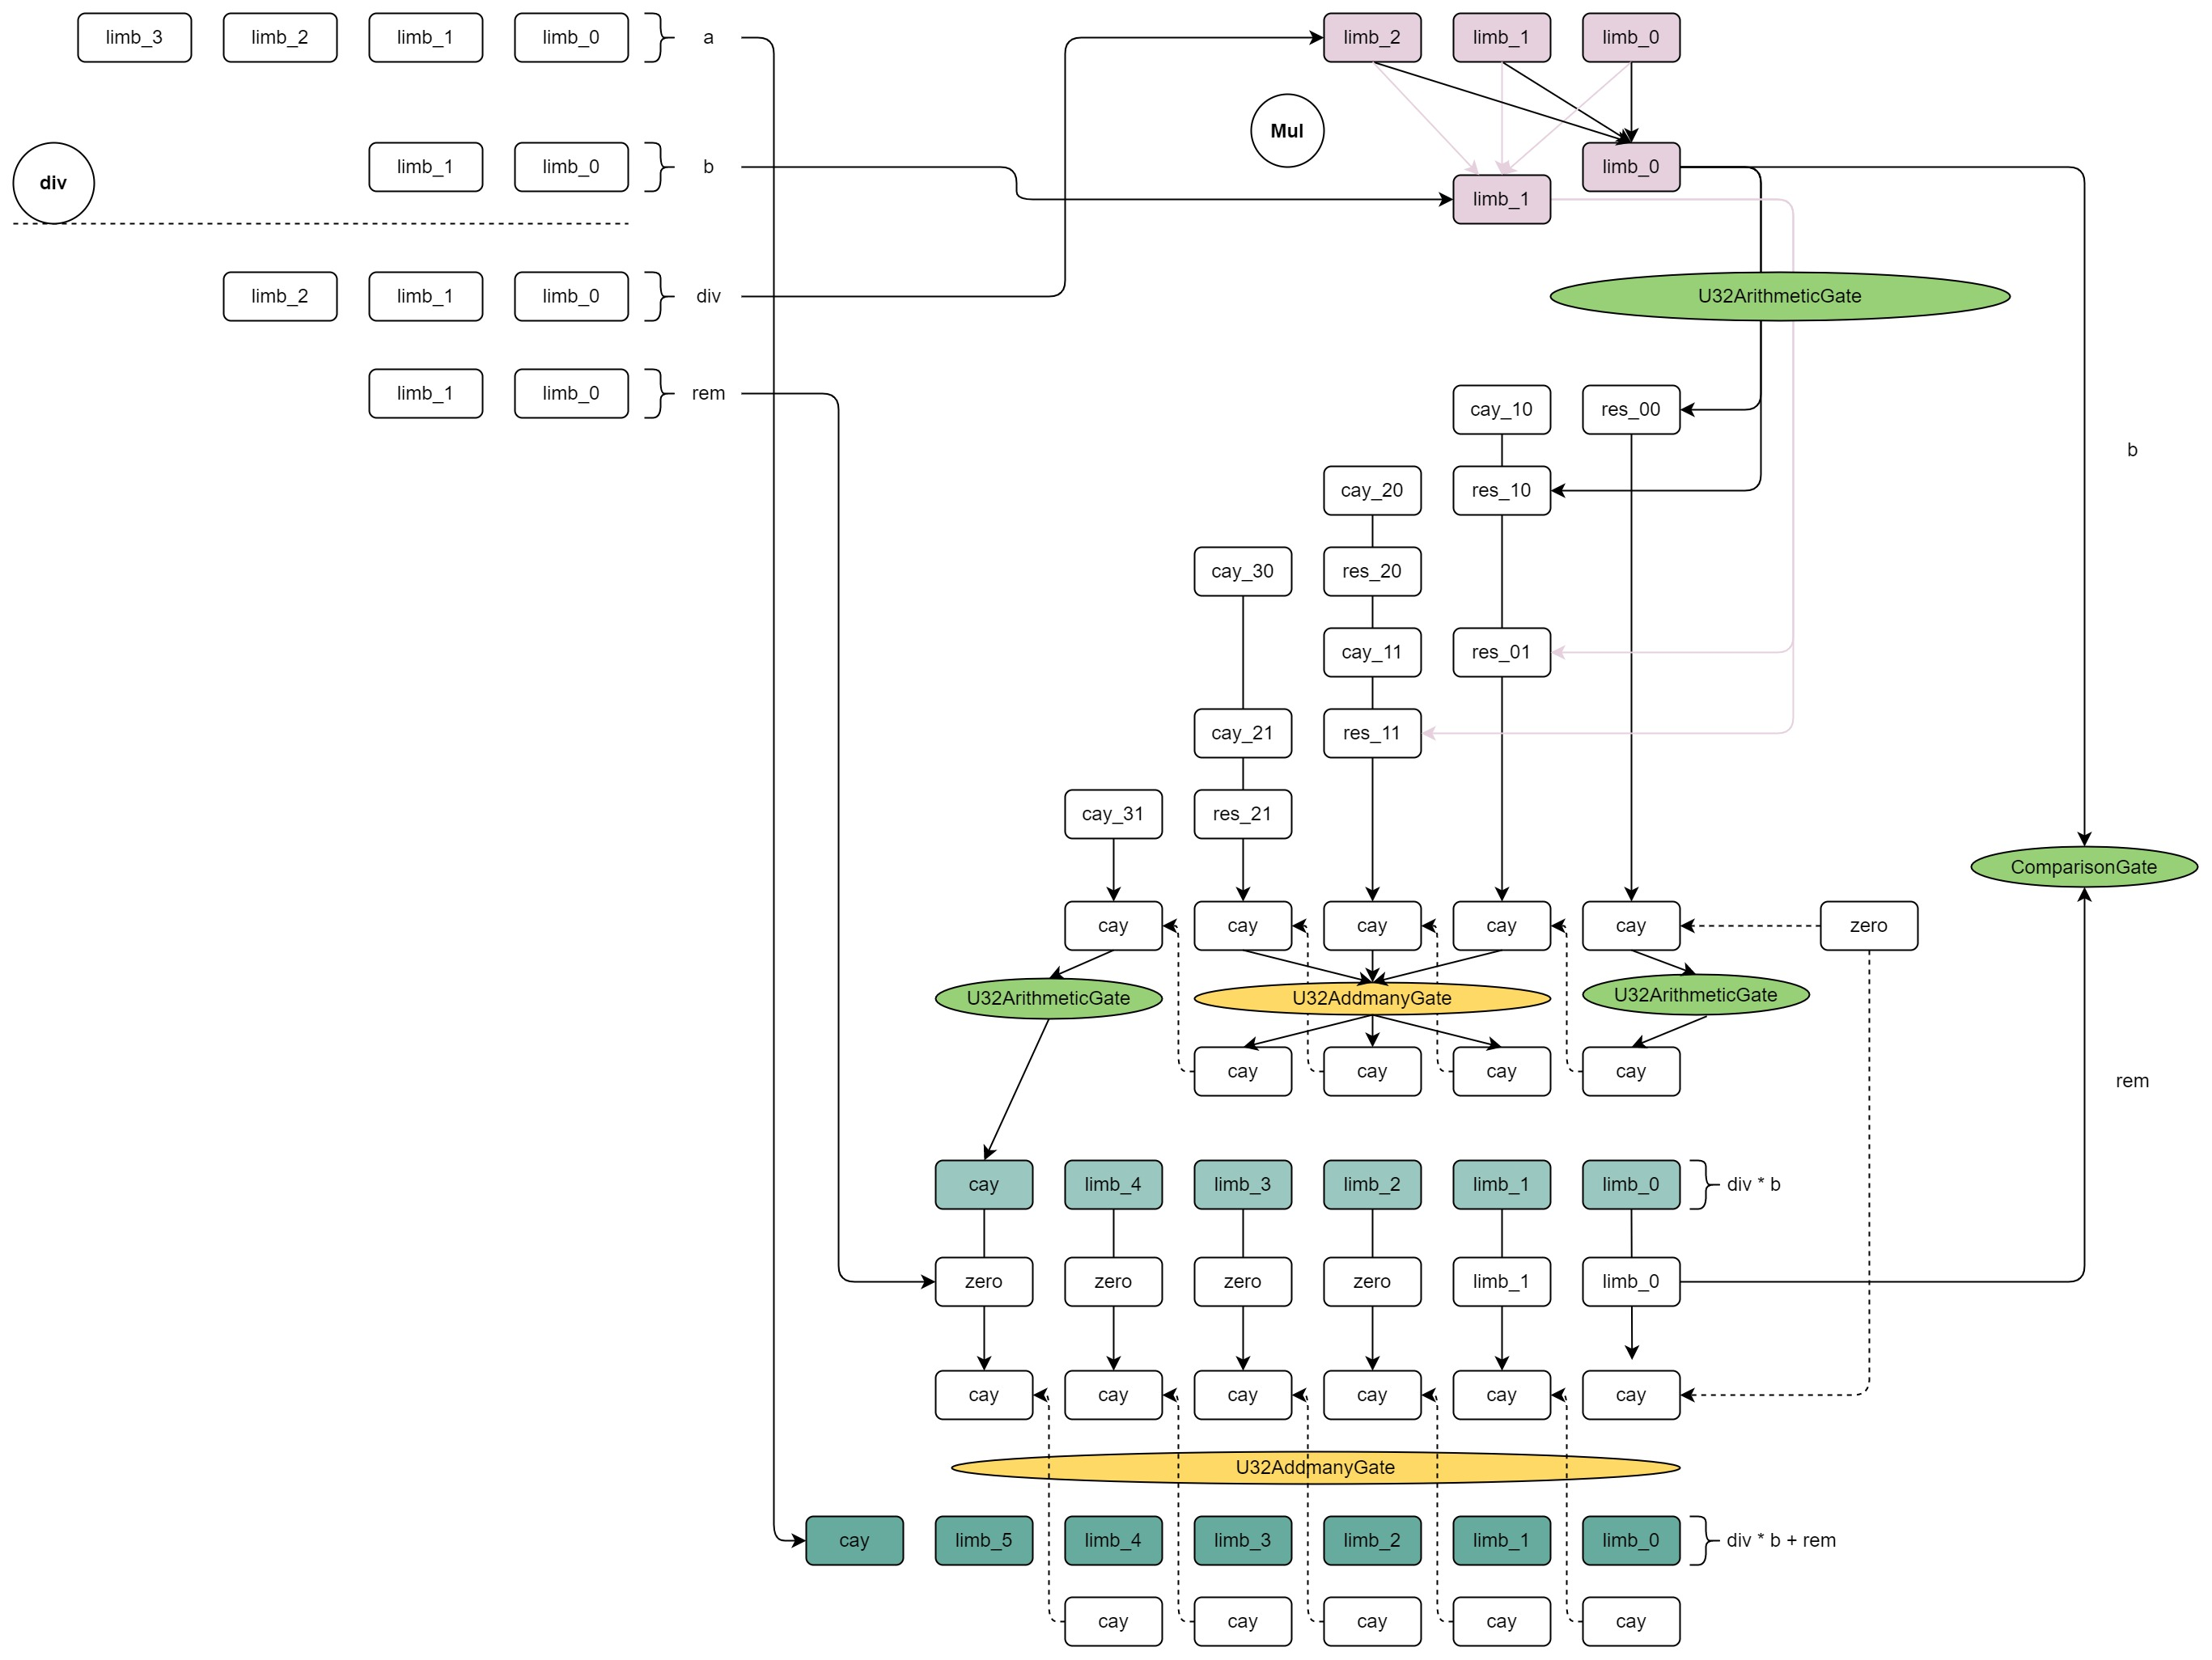
\includegraphics[width=0.8\textwidth]{biguint-div-layout.jpg}
            \caption{biguint-div layout.jpg}
            \label{fig:biguint-div-layout.jpg}
        \end{figure}
    
    \item constraints-info and costs
        \begin{itemize}
            \item Gate type num: 5(U32ArithmeticGate, U32AddManyGate(num-addends: 3), U32AddManyGate(num-addends: 4), ComparisionGate, ArithmeticGate)
            \item Gate instance num: 3 + 3 + 4 + 3 = 13 
            \item U32ArithmeticGate num: 3
            \item U32AddManyGate num: 3
            \item ComparisionGate num: 4
            \item ArithmeticGate num: 3
            \item copy-constraints: 3 * 8 + 4 + 5 + 4 + 4 * 6 + 7 + 1 + 26 + 5 = 100 
            \item max-degree: 4
        \end{itemize}

\end{enumerate}
    \subsubsection{biguint-cmp}

\Par{Target}
Implement the comparison of two biguints.

\Par{Constraints logic}
\begin{itemize}
    \item Split the input to many limbs, such that: \verb|limbs_num = bits / chunks|;
    \item Execute comparison for low bits limbs;
    \item Ensure that the result is determined by the highest limbs which are not equal.
\end{itemize}

\Par{Process layout}
See \figref{fig:biguint-cmp-layout}.
\begin{figure}[!ht]
    \centering
    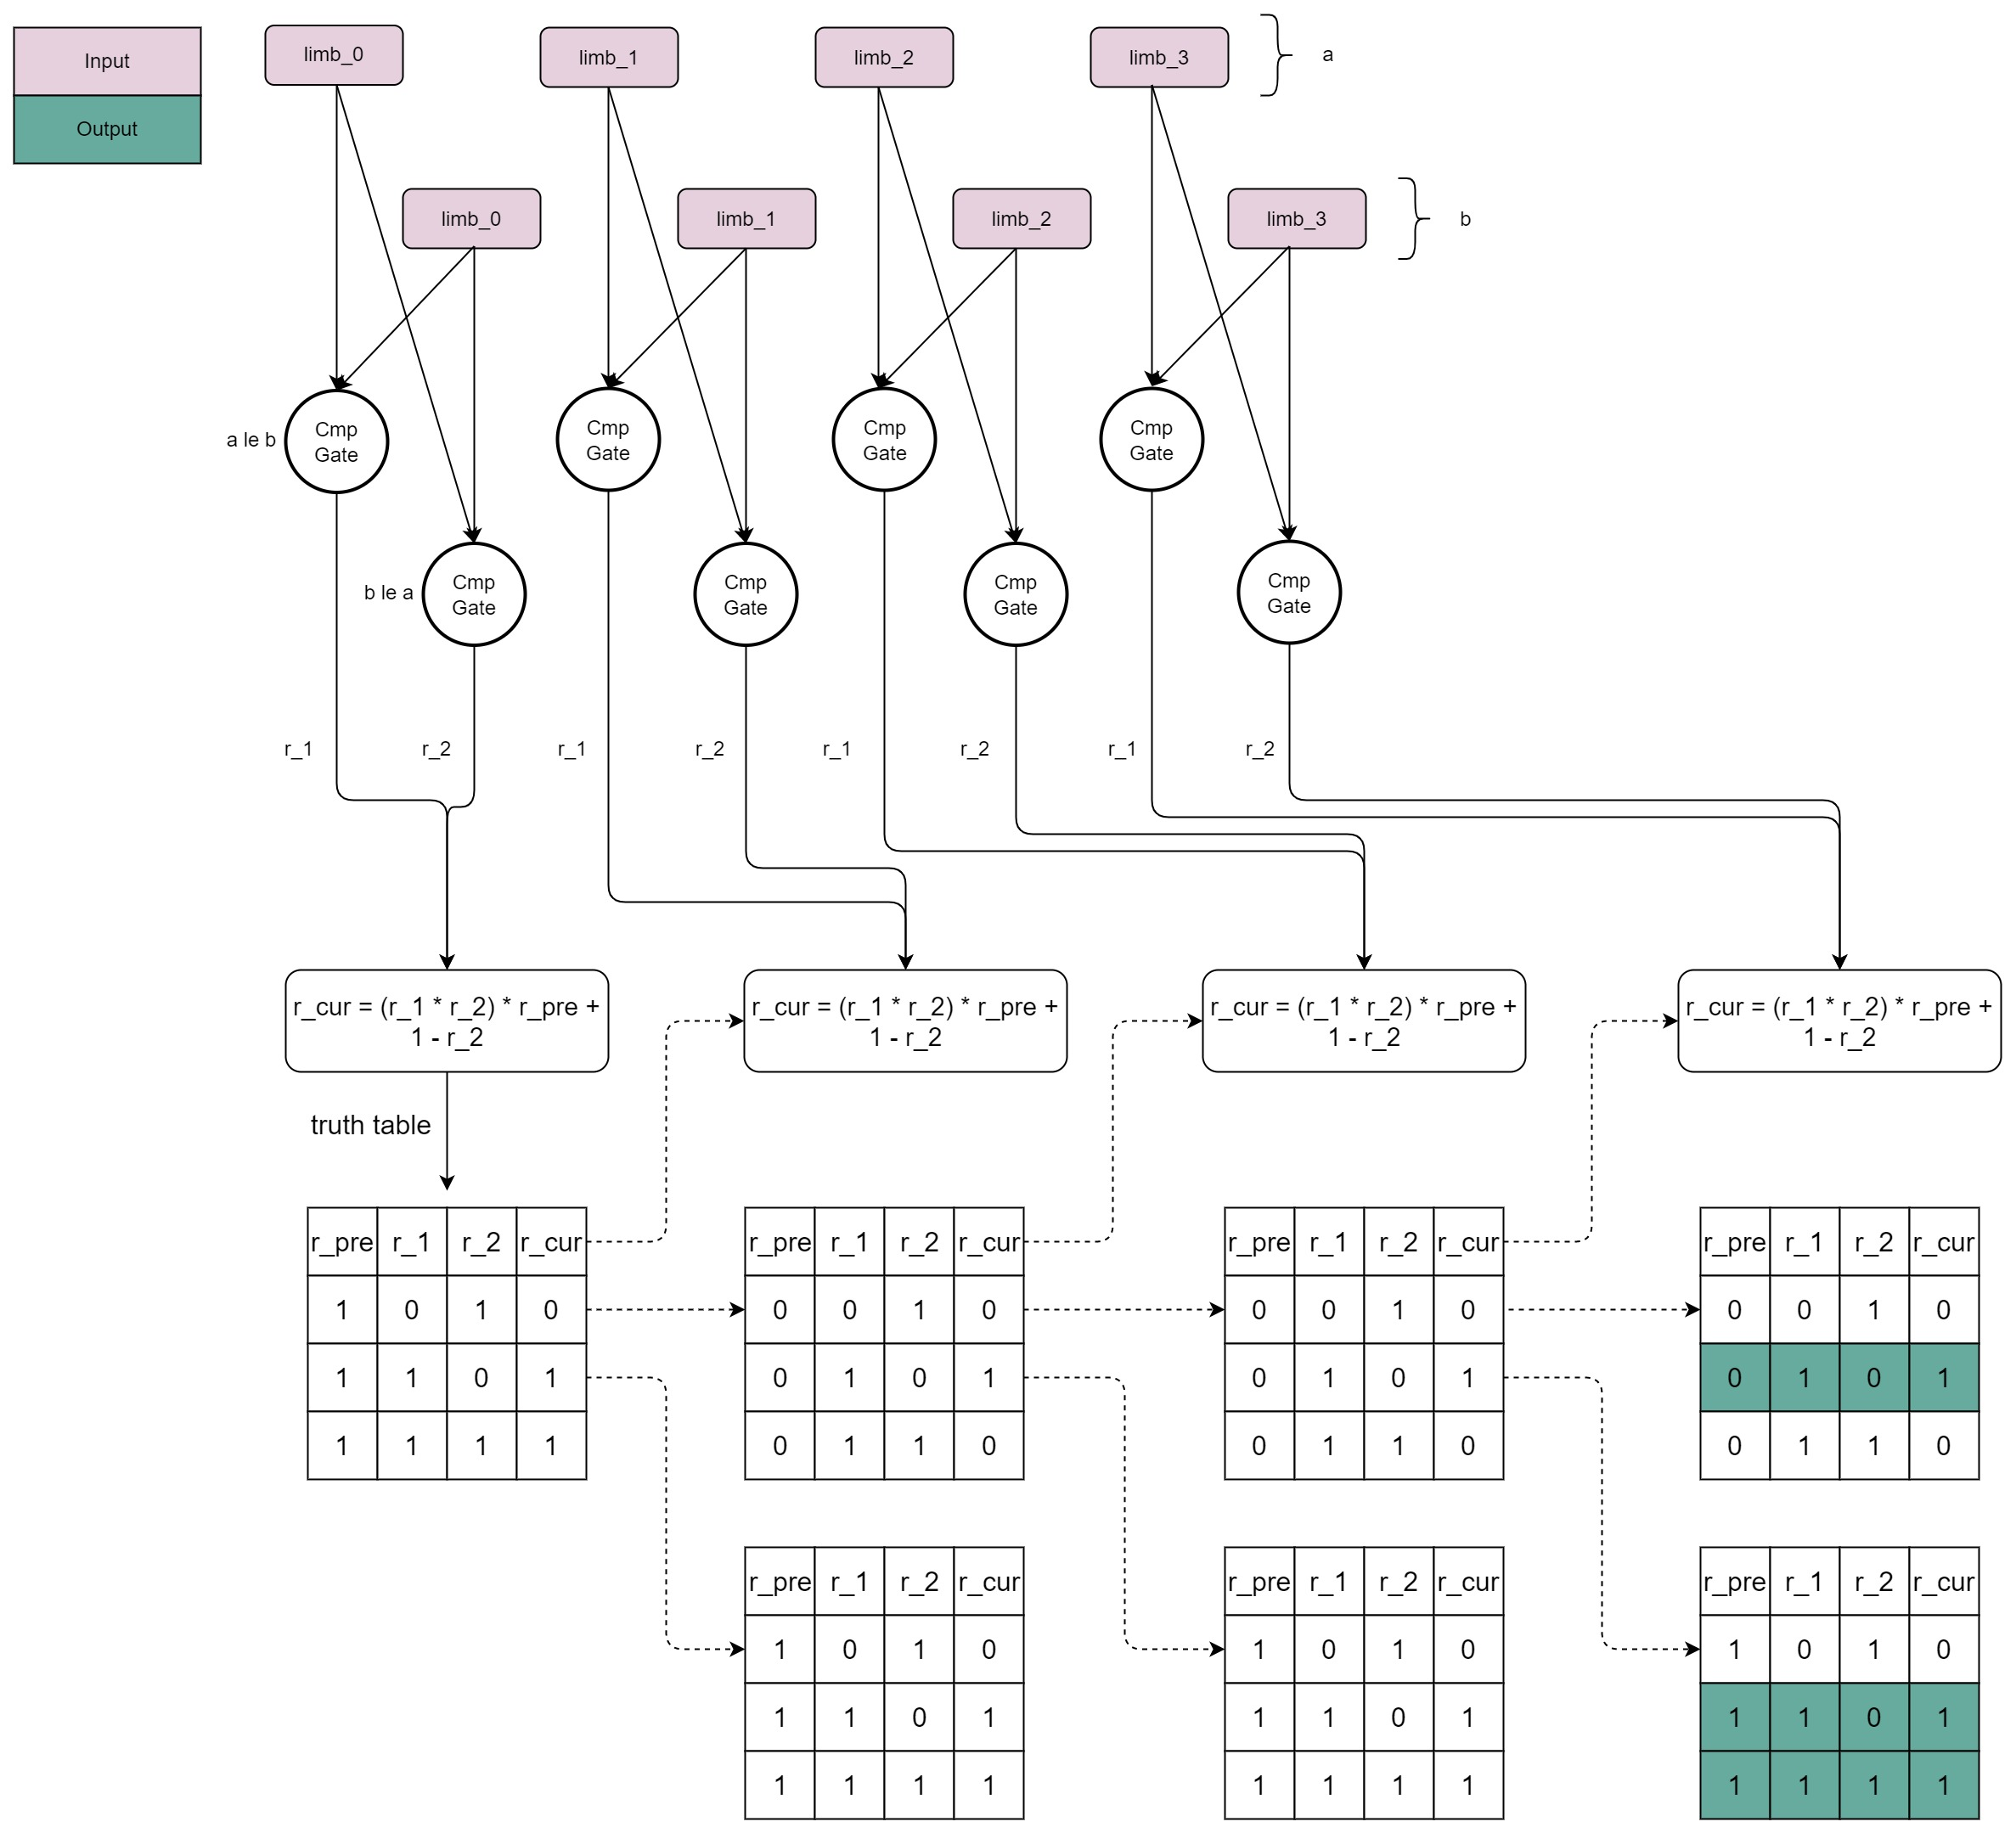
\includegraphics[width=0.8\textwidth]{biguint-cmp-layout.jpg}
    \caption{biguint-cmp layout}
    \label{fig:biguint-cmp-layout}
\end{figure}

\Par{Circuit layout}
See \figref{fig:biguint-cmp-circuit-layout}.
\begin{figure}[!ht]
    \centering
    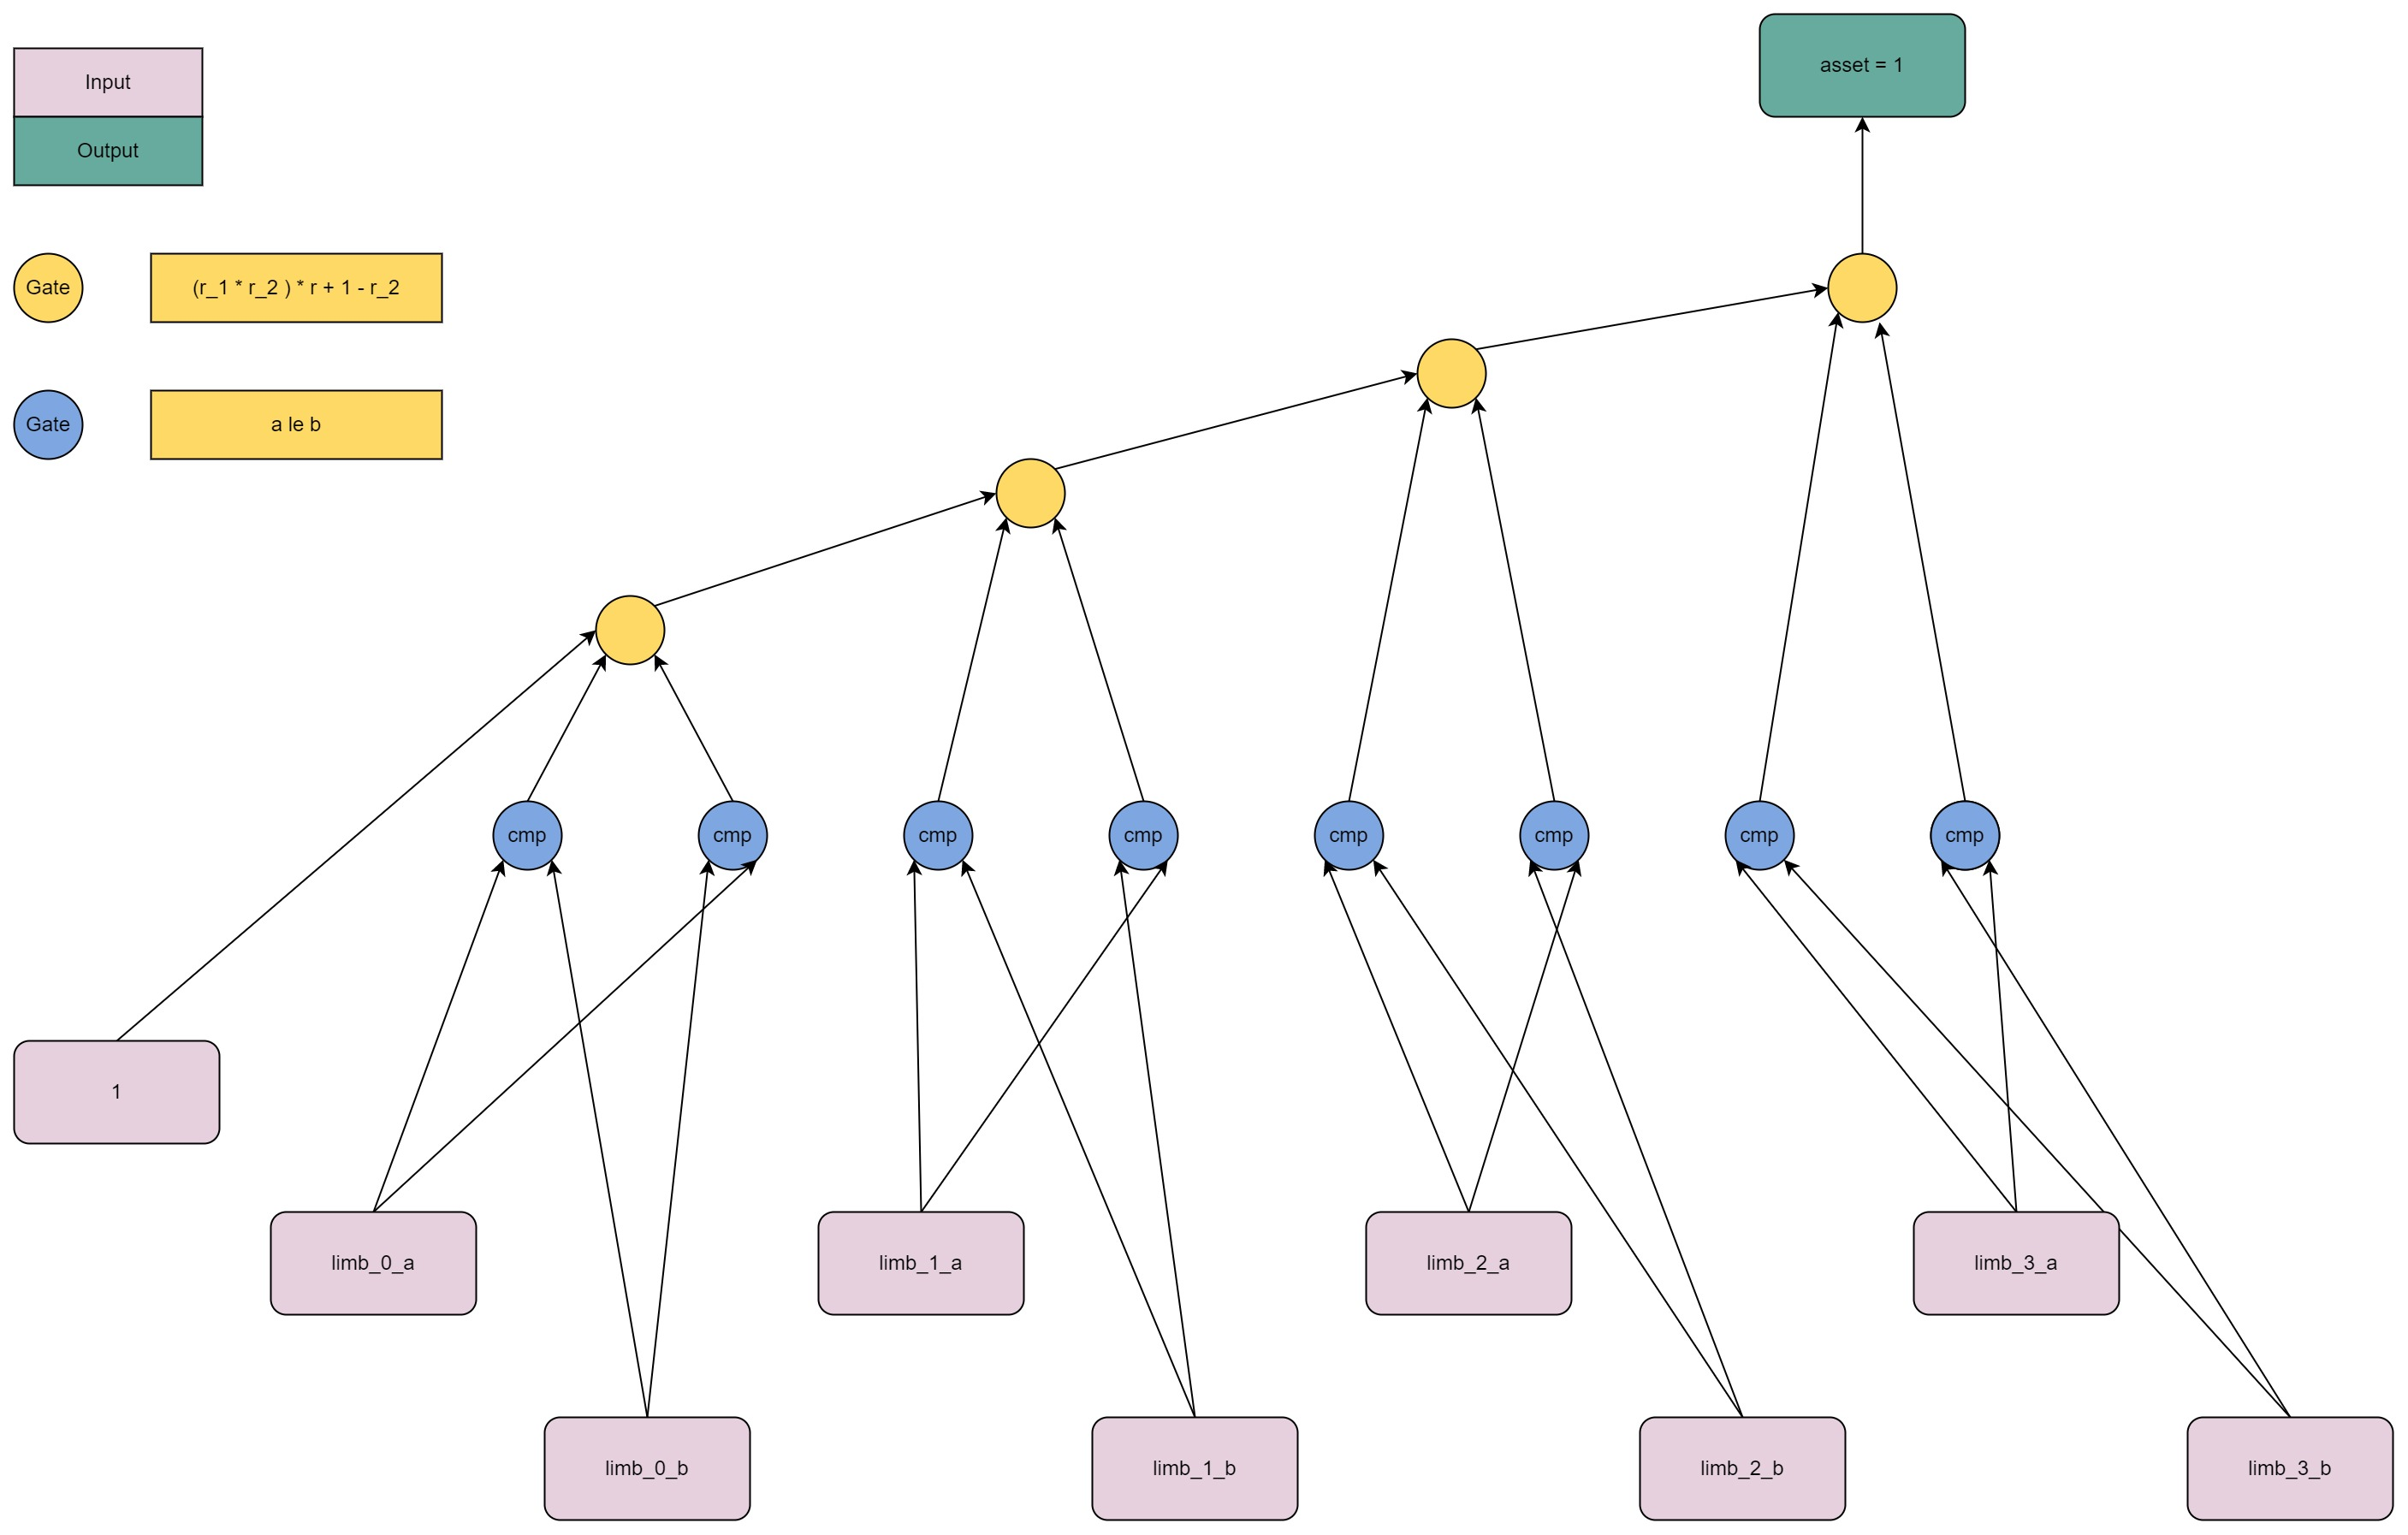
\includegraphics[width=0.8\textwidth]{biguint-cmp-circuit-layout.jpg}
    \caption{biguint-cmp circuit layout}
    \label{fig:biguint-cmp-circuit-layout}
\end{figure}

\Par{Constraints info and costs}
\begin{itemize}
    \item Gate type num: 2 (ComparisionGate, ArithmeticGate)
    \item Gate instance num: $4 \times 2 + 3 = 11$
    \item ComparisionGate num: 8
    \item ArithmeticGate num: 3
    \item copy-constraints: $(4 + 9) \times 4 + 1 = 53$
    \item max-degree: 4
\end{itemize}

    \subsubsection{nonnative-add}
\label{nonnative-add}

\begin{enumerate}
    \item target
        check the additional relation among three nonnative target objects.
    \item constraints-logic
        \begin{itemize}
            \item check equation for gadget,  a + b = c + modular * overflow
            \item check that "c lt modular"
        \end{itemize}
    \item nonnative-add process layout
        \begin{figure}[!ht]
            \centering
            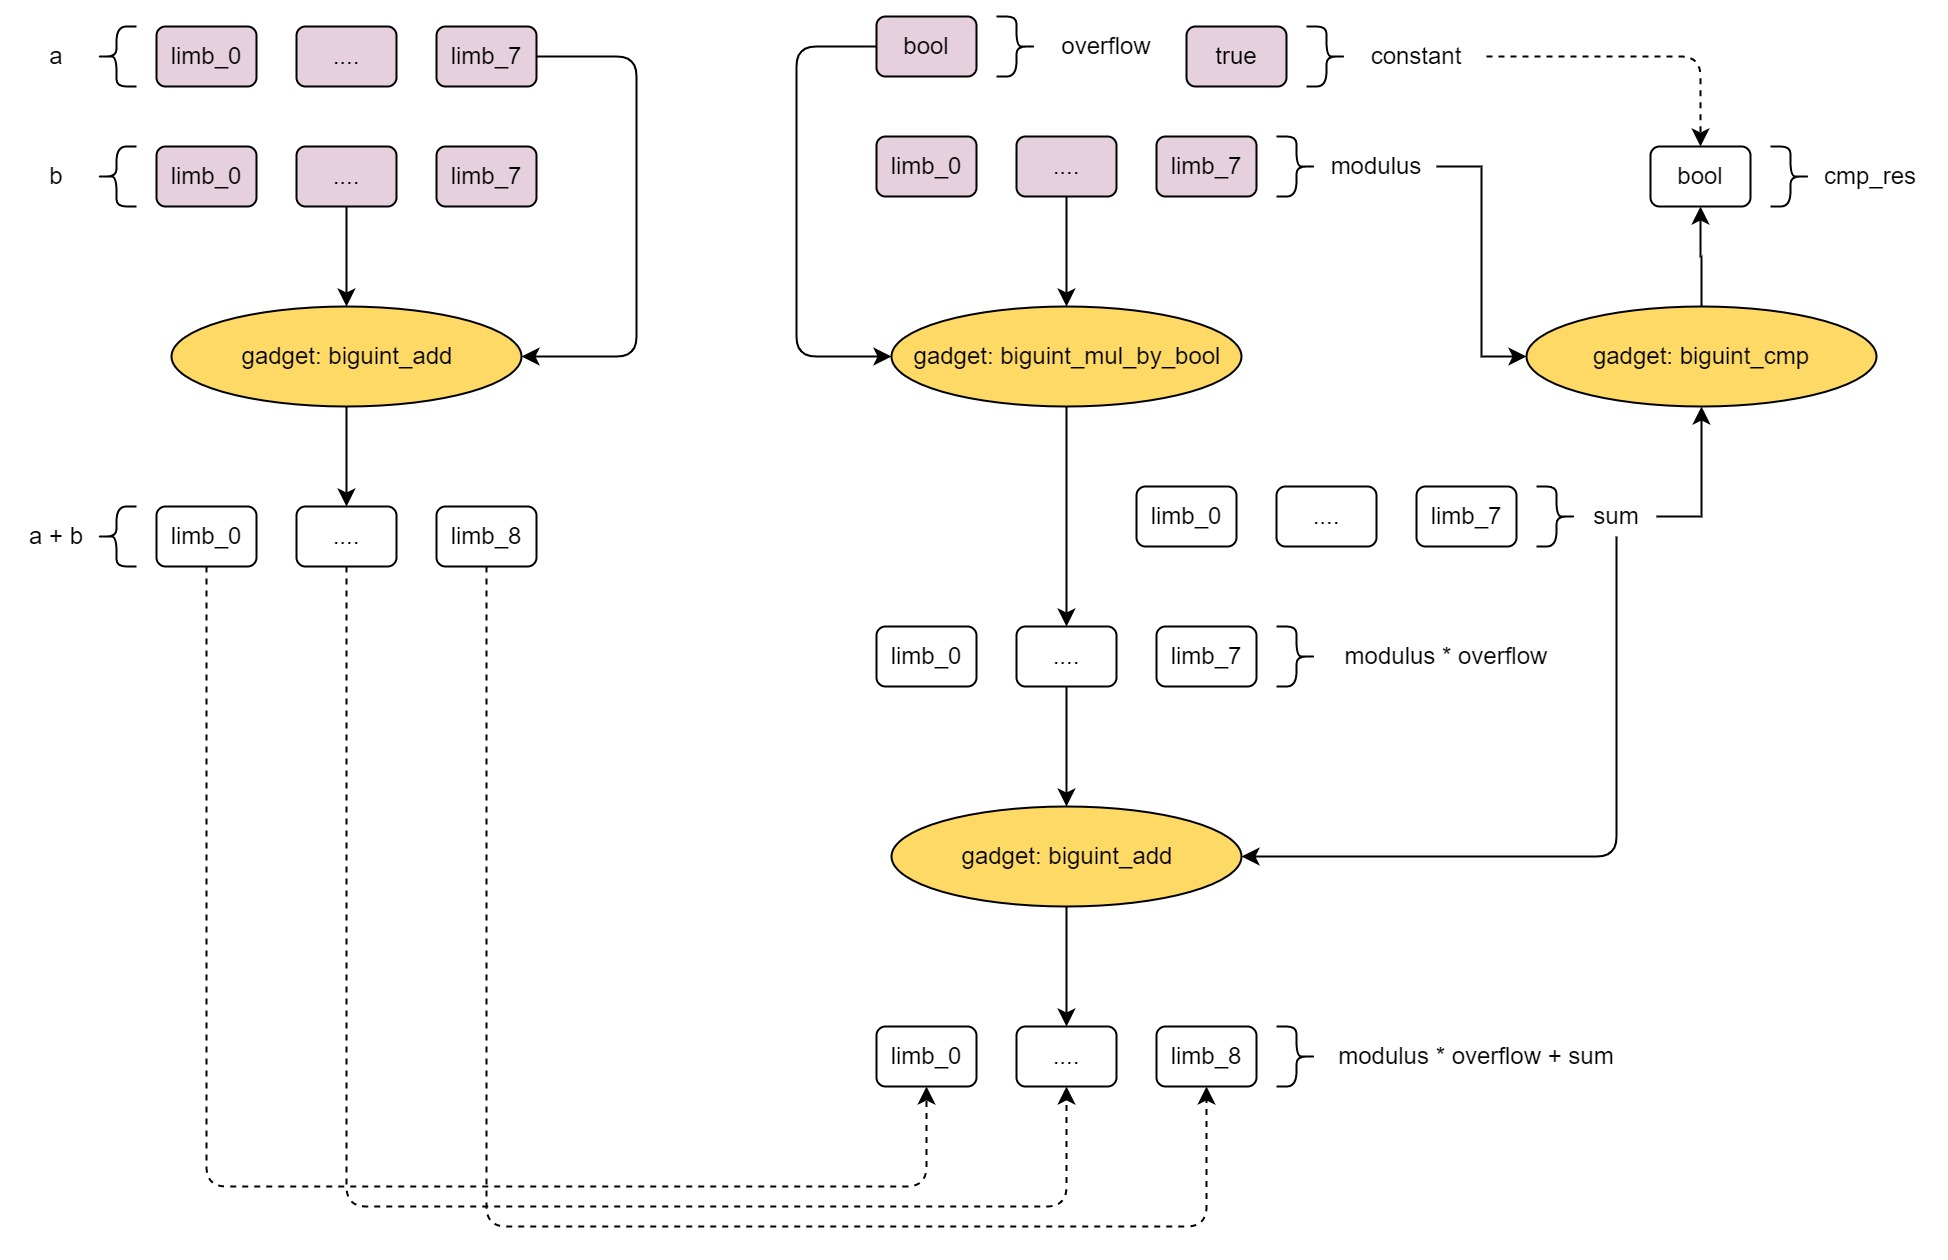
\includegraphics[width=0.8\textwidth]{nonnative-add-layout.jpg}
            \caption{nonnative-add layout}
            \label{fig:nonnative-add-layout}
        \end{figure}
    
    \item constraints-info and costs
        \begin{itemize}
            \item gadget biguint-add num: 2
            \item gadget biguint-mul-by-bool num: 1
            \item gadget biguint-cmp num: 1
            \item gate type num: 3(U32AddManyGate, ComparisonGate, ArithmeticGate)
            \item gate instance num: 23 = 3(U32AddManyGate) + 16(ComparisonGate) + 2(ArithmeticGate(1,0)) + 1(ArithmeticGate(1,-1)) + 1(ArithmeticGate(1,1))
            \item copy-constraints: 186 = 32 * 2{biguint-add} + 9{biguint-mul-by-bool} + 9 + (4 + 9) * 8{biguint-cmp} = 186
        \end{itemize}

    \item questions
        \begin{itemize}
            \item when set value to sum?
        \end{itemize}

\end{enumerate}
    \subsubsection{nonnative-sub}
\label{nonnative-sub}

\begin{enumerate}
    \item target
        check the substract relation among three nonnative target objects.
    \item constraints-logic
        \begin{itemize}
            \item check equation for gadget,  diff + b = a + modular * overflow
            \item check that "overflow is bool"
            \item check that "diff.limbs is range U32"
        \end{itemize}
    \item nonnative-sub process layout
        \begin{figure}[!ht]
            \centering
            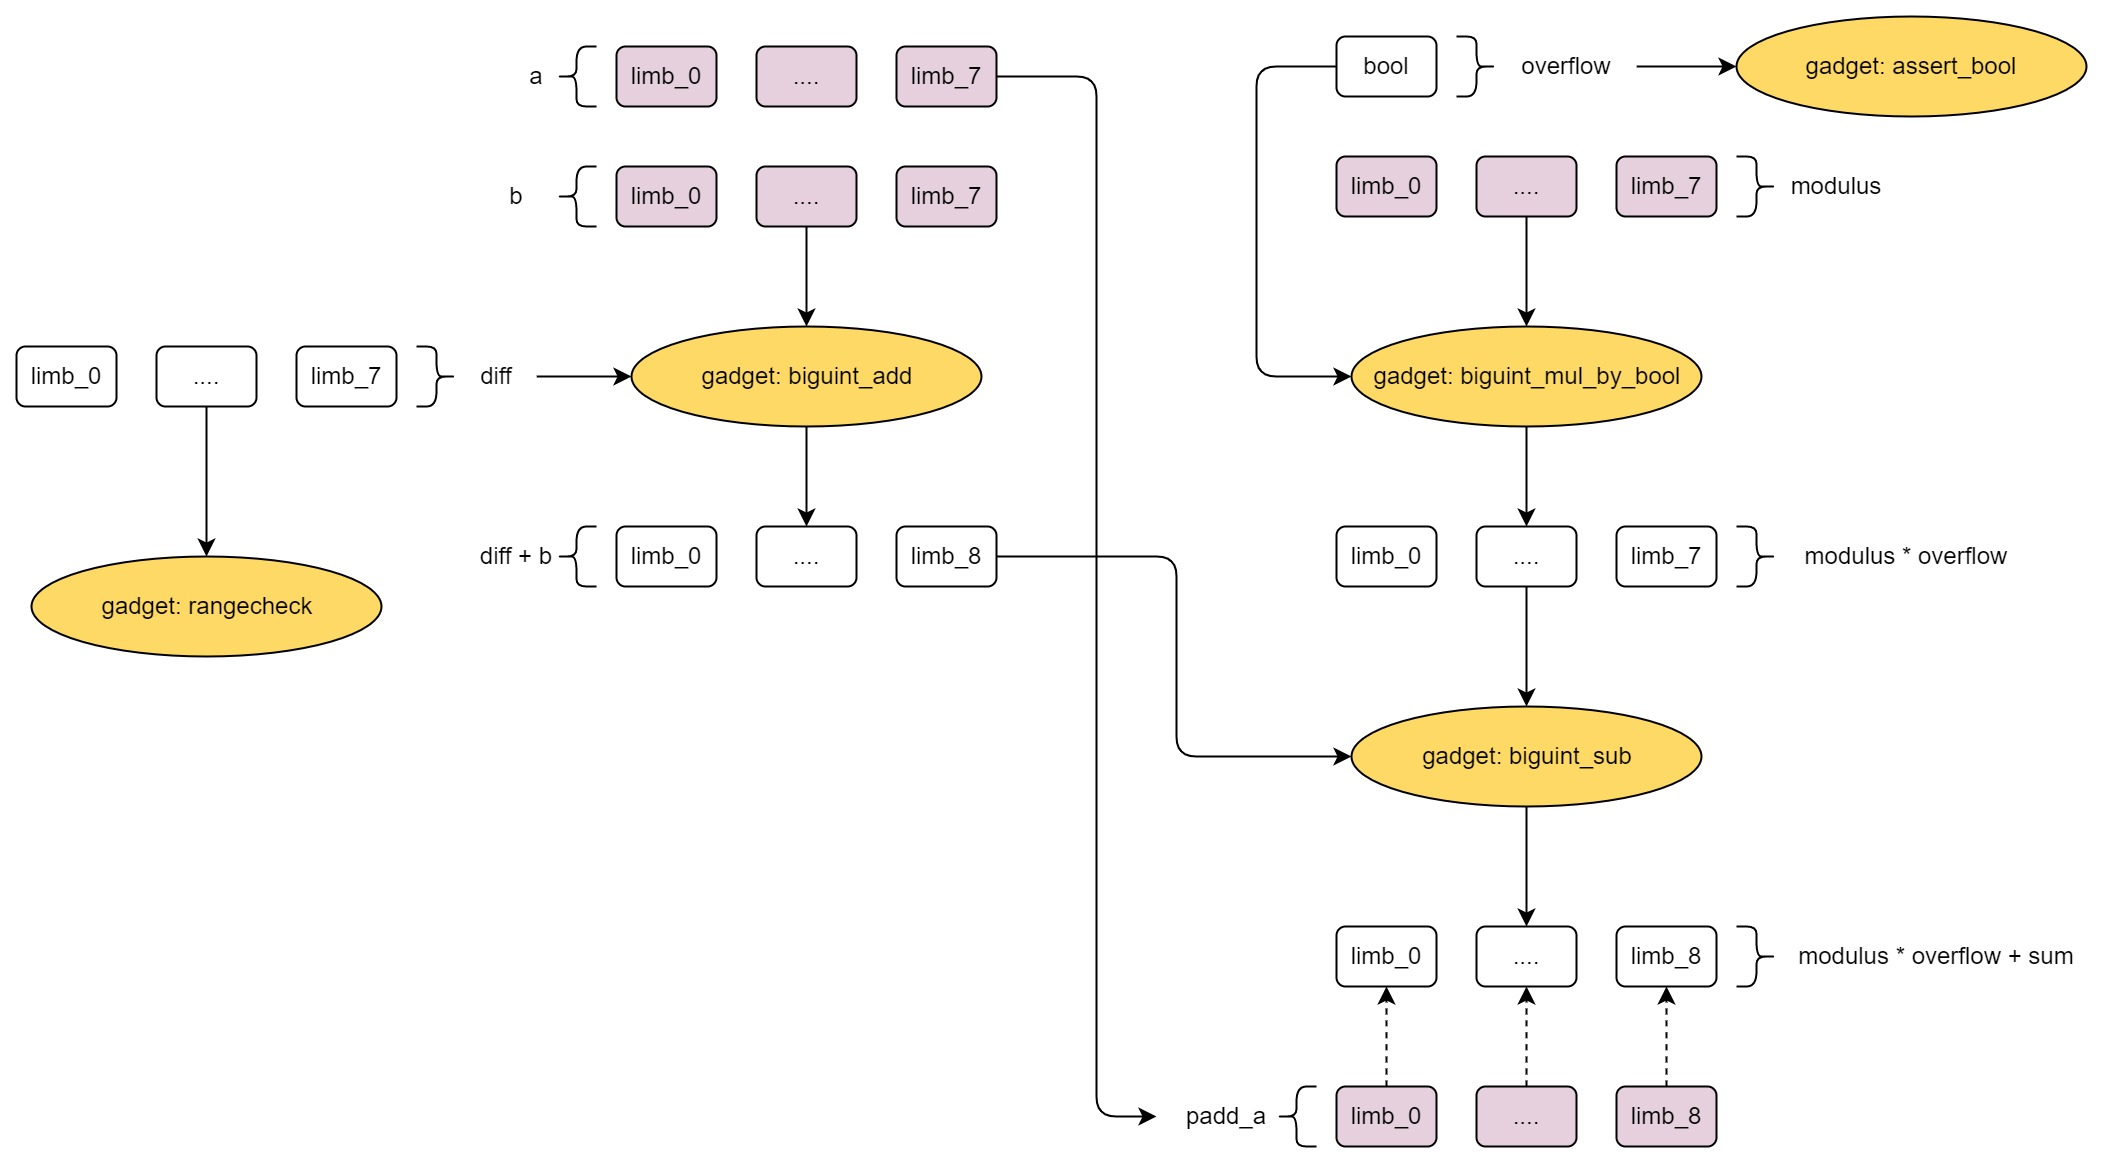
\includegraphics[width=0.8\textwidth]{nonnative-sub-layout.jpg}
            \caption{nonnative-sub layout}
            \label{fig:nonnative-sub-layout}
        \end{figure}
    
    \item constraints-info and costs
        \begin{itemize}
            \item gadget biguint-add num: 1
            \item gadget biguint-sub num: 1
            \item gadget biguint-mul-by-bool num: 1
            \item gadget u32rangecheck num: 1
            \item gadget assert-bool num: 1
            \item gate type num: 4(U32AddManyGate, U32SubtractionGate, U32RangeCheckGate, ArithmeticGate)
            \item gate instance num: 7 = 2(U32AddManyGate) + 2(U32SubtractionGate) + 1(U32RangeCheckGate) + 1(ArithmeticGate(1,0)) + 1(ArithmeticGate(1,-1))
            \item copy-constraints: 89 = 32{biguint-add num} + 27{U32SubtractionGate} + 9{biguint-mul-by-bool} + 8{u32rangecheck} + 4{assert-bool} + 9
        \end{itemize}

    \item questions
        \begin{itemize}
            \item why not constraint for overflow at nonnative-add?
            \item why not make u32rangecheck for input at nonnative-add?
        \end{itemize}

\end{enumerate}
    \subsubsection{nonnative-mul}
\label{nonnative-mul}

\begin{enumerate}
    \item target
        check the multiplicatipn relation among three nonnative target objects.
    \item constraints-logic
        \begin{itemize}
            \item check equation for gadget,  a * b = prod + modular * overflow
            \item check that "overflow.limb is U32"
            \item check that "prod.limb is U32"
        \end{itemize}
    \item nonnative-mul process layout
        \begin{figure}[!ht]
            \centering
            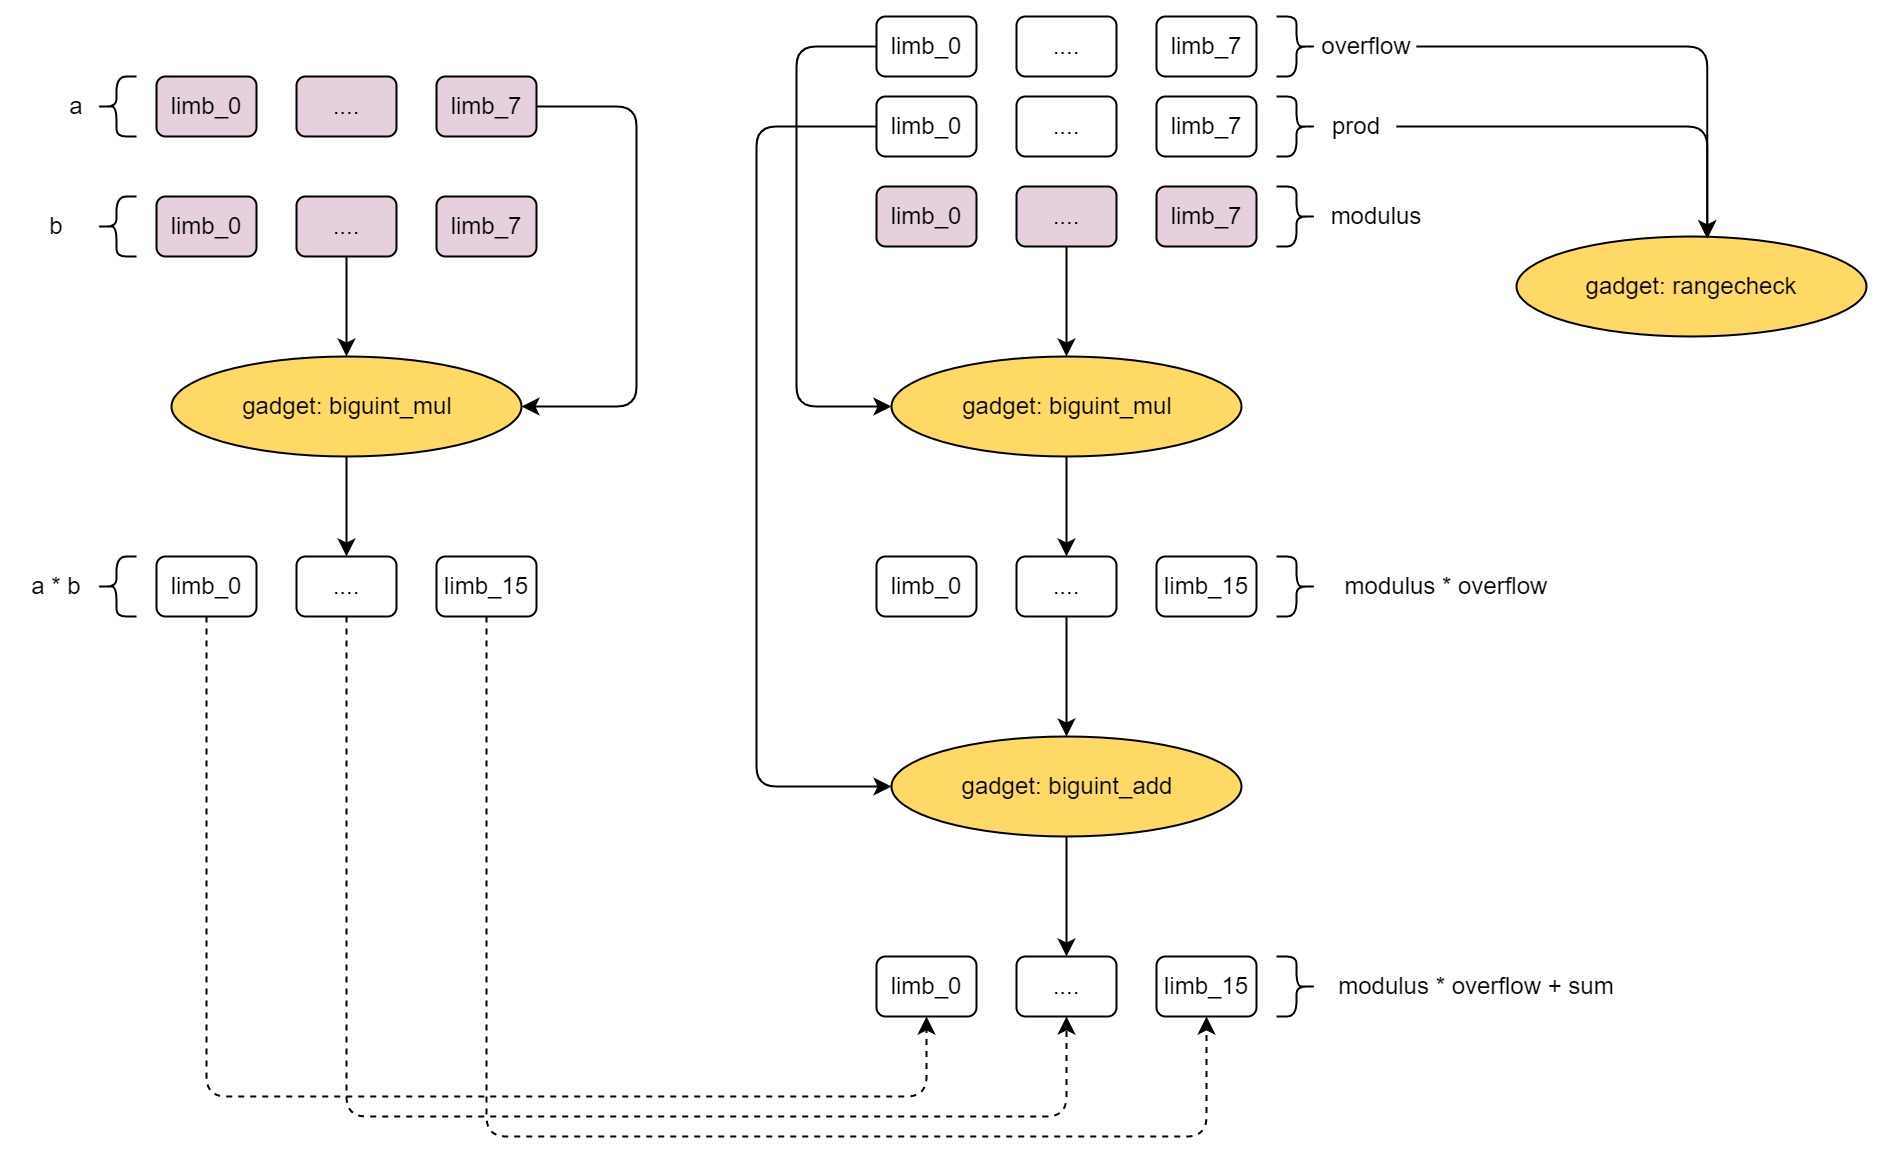
\includegraphics[width=0.8\textwidth]{nonnative-mul-layout.jpg}
            \caption{nonnative-mul layout}
            \label{fig:nonnative-mul-layout}
        \end{figure}
    
    \item constraints-info and costs
        \begin{itemize}
            \item gadget biguint-add num: 1
            \item gadget biguint-mul num: 2
            \item gadget u32rangecheck num: 2
            \item gate type num: 9 = 7(U32AddManyGate{3,5,7,9,11,13,15}) + 1(U32RangeCheckGate) + 1(U32ArithmeticGate)
            \item gate instance num: 37 = 2(u32rangecheck) + 8(biguint-mul: constant-input) + 22(biguint-mul) + 1 + 3(biguint-add)
            \item copy-constraints: 583 = 8 * 2(u32rangecheck) + 3 * 3 + (4 + 6 + 8 + 10 + 12 + 14 + 16) * 4 + (8 * 8) * 3 + 17 * 4 + 18
        \end{itemize}

\end{enumerate}
    \subsubsection{nonnative-inv}

\Par{Target}
Check the modular inverse relation among three nonnative target objects.

\Par{Constraints logic}
\begin{itemize}
    \item Check equation for gadget: \verb|a * inv_a = 1 + modular * div|.
\end{itemize}

\Par{Process layout}
See \figref{fig:nonnative-inv-layout}.
\begin{figure}[!ht]
    \centering
    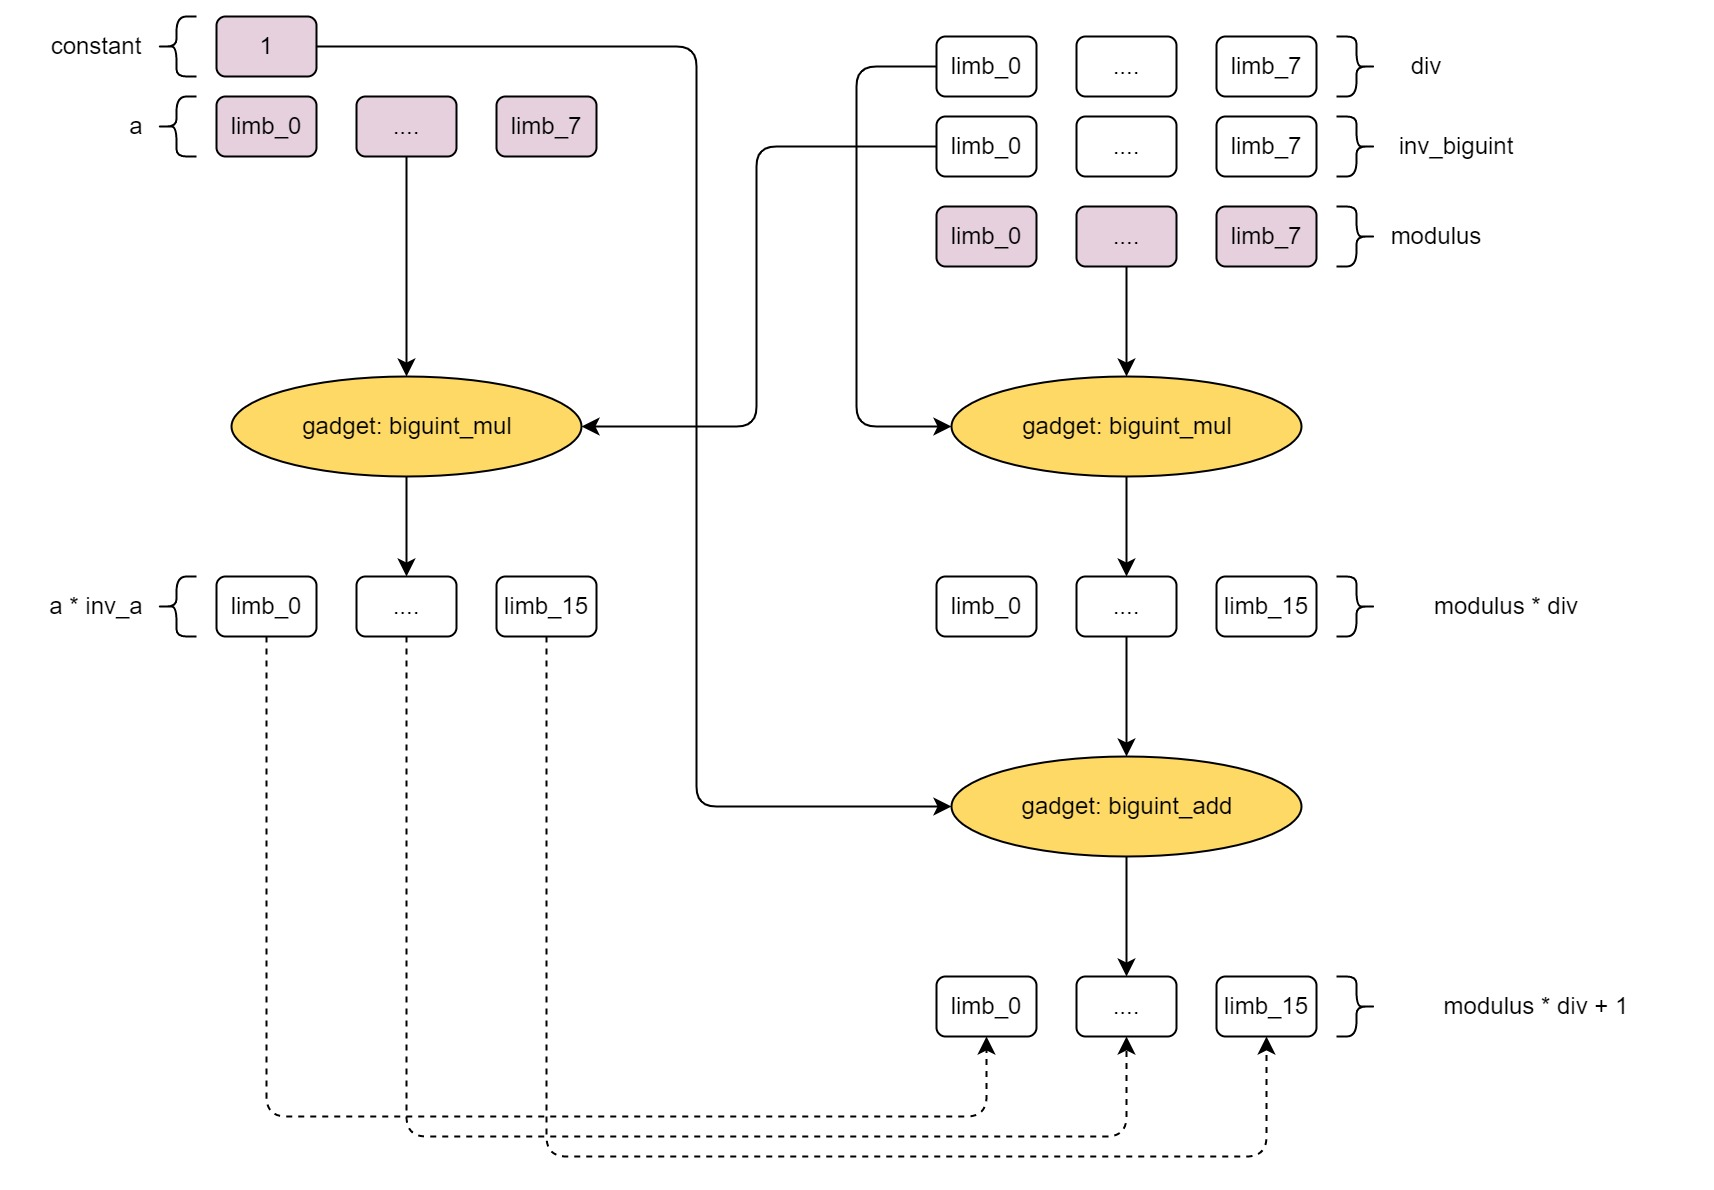
\includegraphics[width=0.8\textwidth]{nonnative-inv-layout.jpg}
    \caption{nonnative-inv layout}
    \label{fig:nonnative-inv-layout}
\end{figure}

\Par{Constraints info and costs}
\begin{itemize}
    \item gadget biguint-add num: 1
    \item gadget biguint-mul num: 2
    \item gate type num: 8 = 7(U32AddManyGate\{3,5,7,9,11,13,15\}) + 1(U32ArithmeticGate)
    \item gate instance num: 56 = (8 * 8 + 2) * 2 / 3 + 5(U32AddManyGate{3}) + 5 + 2(U32AddManyGate{15})
    \item copy-constraints: 762 = (8 * 8 + 2) * 2 * 3 + 21 * 4 + (6 + 8 + 10 + 12 + 14) * 4 + 4 * 16 + 18
\end{itemize}

    \section{curve-add}
\label{curve-add}

Take curve-secp256k1 as example, the same as other texs.

\begin{enumerate}
    \item target
        implement the addition of two different curve points. this is a incomplete addition, you can refer to The halo2 Book \cite{website:halo2-book} to learn more about it.
    \item constraints-logic
        \begin{figure}[!ht]
            \centering
            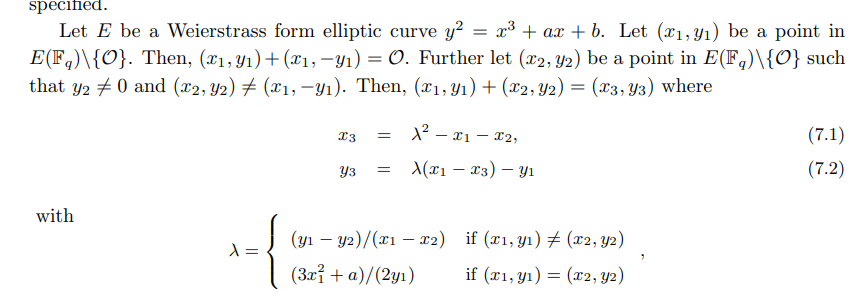
\includegraphics[width=0.8\textwidth]{curve-add.jpg}
            \caption{curve-add}
            \label{fig:curve-add}
        \end{figure}
    \item curve-add process layout
        \begin{figure}[!ht]
            \centering
            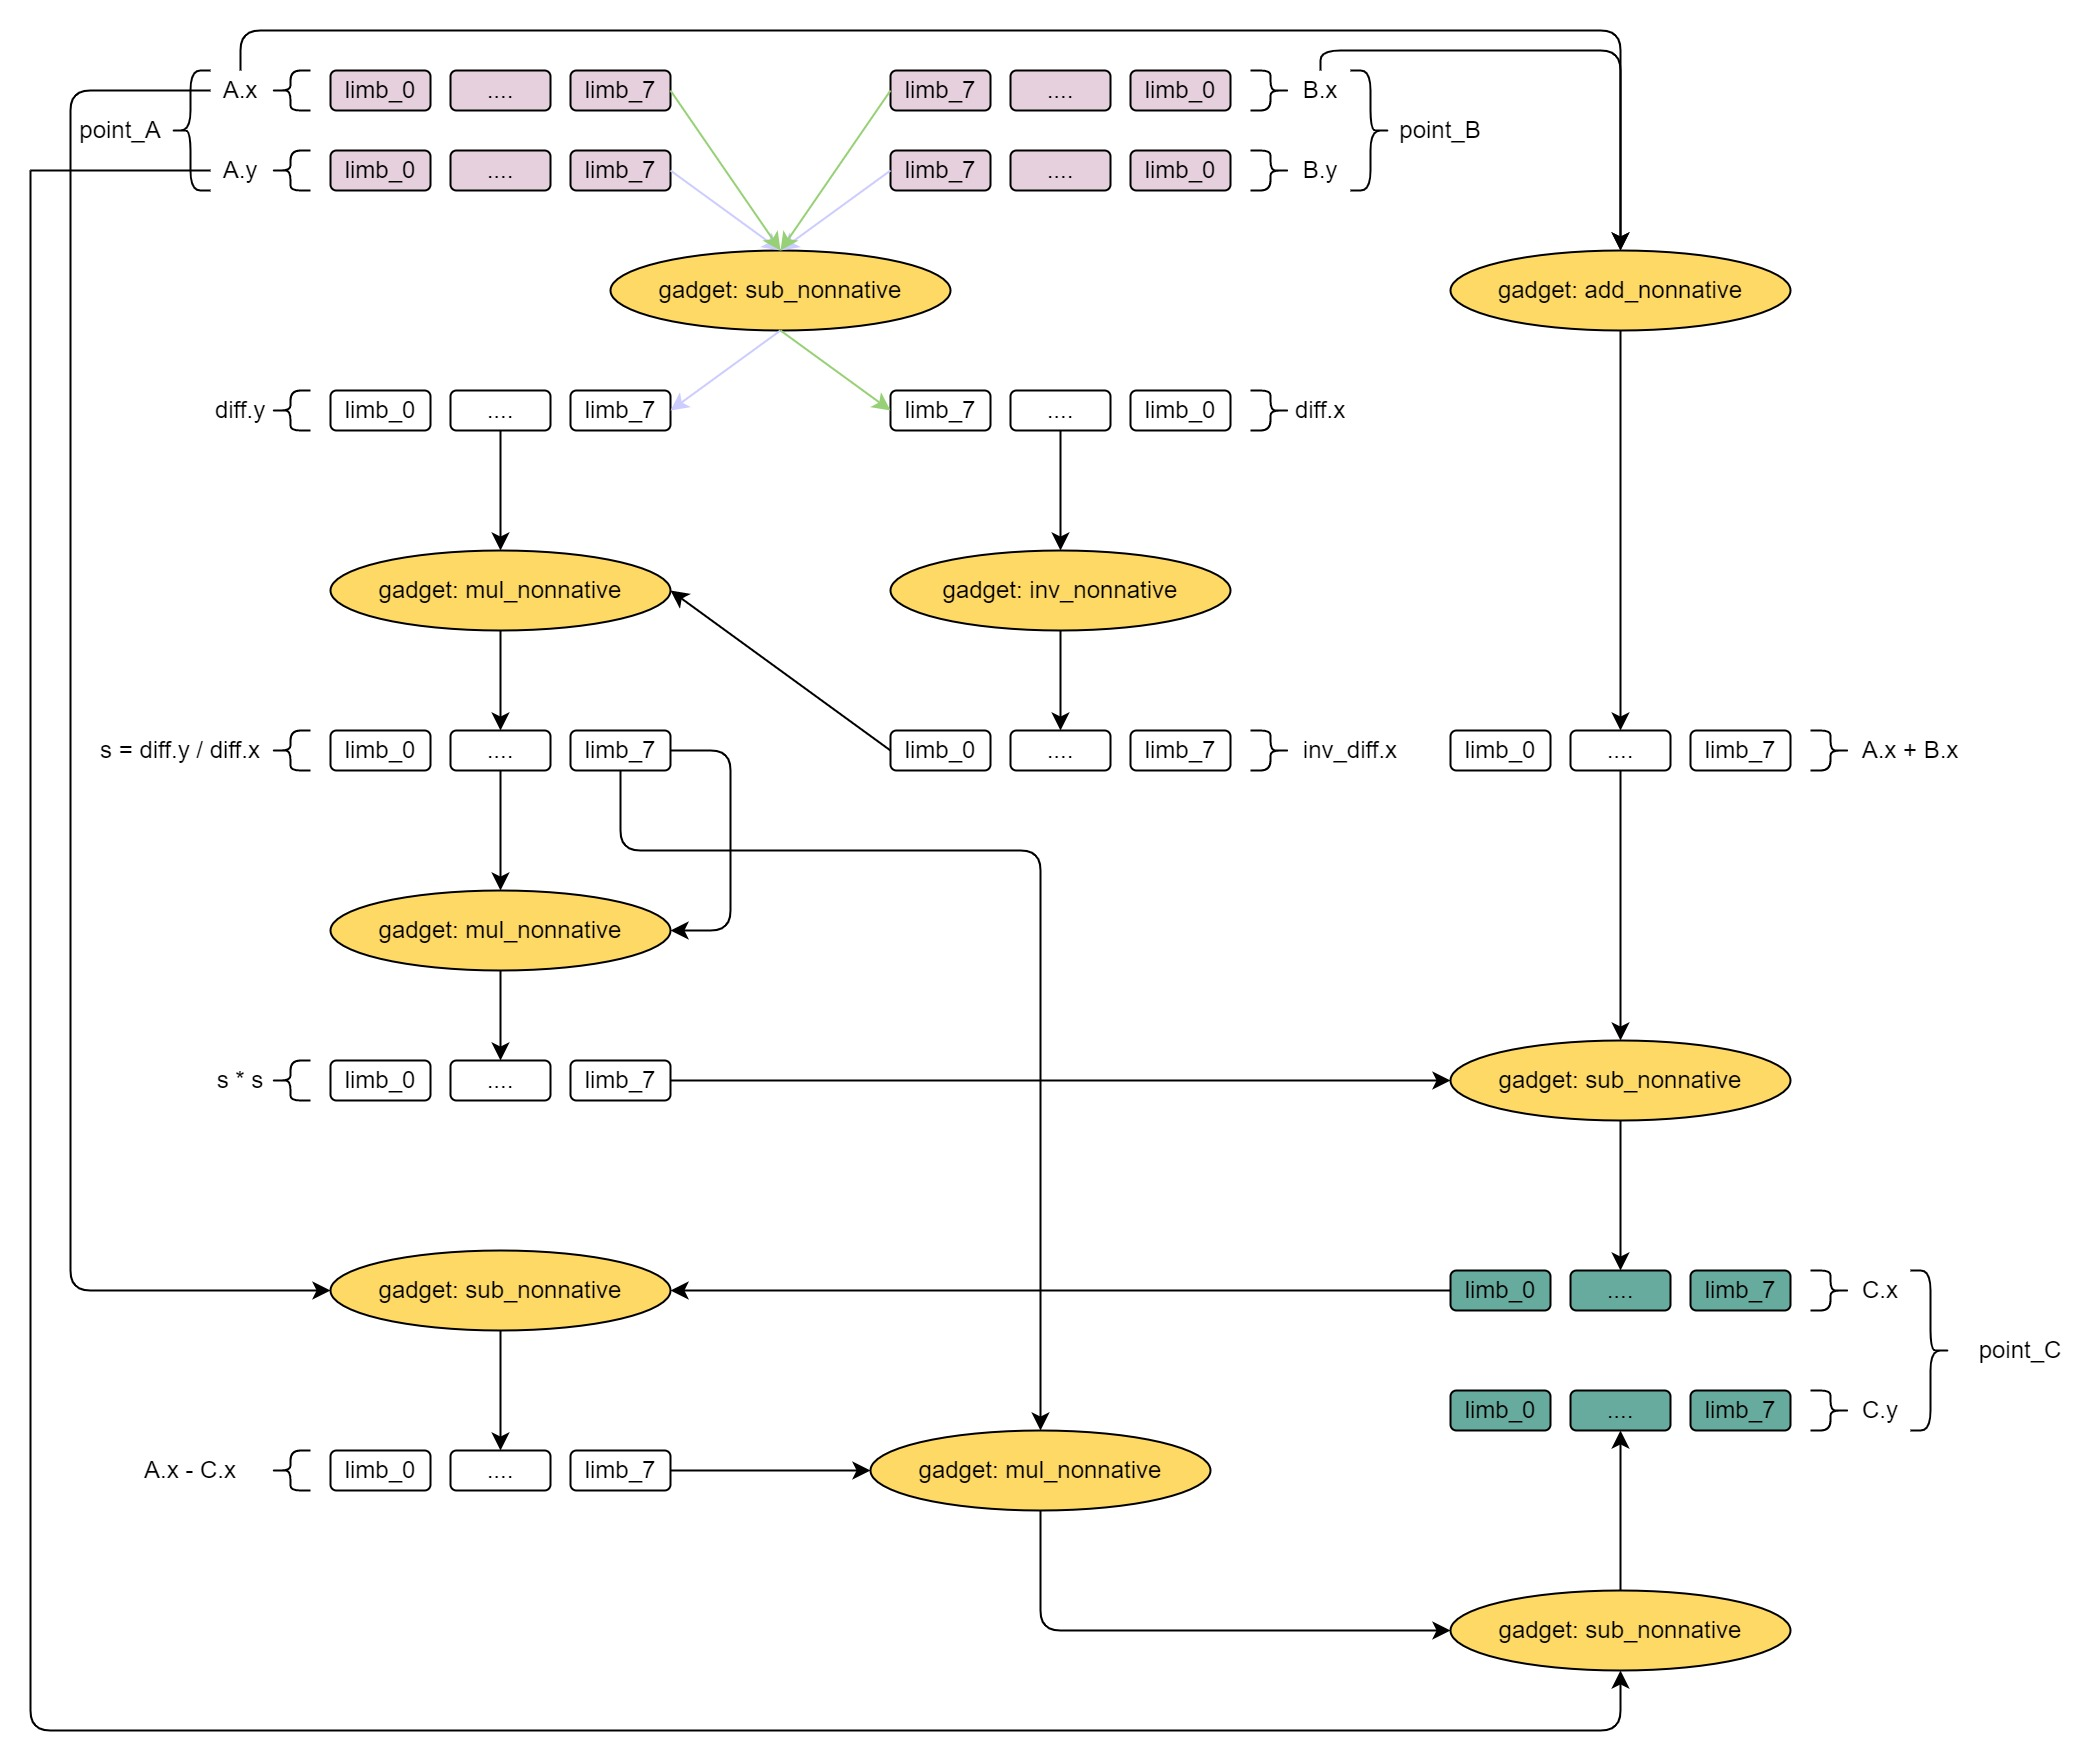
\includegraphics[width=0.8\textwidth]{curve-add-layout.jpg}
            \caption{curve-add layout}
            \label{fig:curve-add-layout}
        \end{figure}
    
    \item constraints-info and costs
        \begin{itemize}
            \item gadget-sub-nonnative num: 5
            \item gadget-add-nonnative num: 1
            \item gadget-mul-nonnative num: 3
            \item gadget-inv-nonnative num: 1
            \item gate type num: 
            \item gate instance num: 
        \end{itemize}

\end{enumerate}
    %\printbibliography[heading=bibintoc, title=\ebibname]%
\end{document}
 
    \documentclass{elegantpaper}
\usepackage{datetime2}
\usepackage[T1]{fontenc}
\usepackage{graphicx}
\usepackage{listings}

\DTMusemodule{english}{en-GB}
\DTMnewdatestyle{short}{
  \renewcommand{\DTMdisplaydate}[4]{
    \DTMenglishmonthname{##2} \number##1\relax
  }
  \renewcommand{\DTMDisplaydate}{\DTMdisplaydate}
}
\newcommand{\shorttoday}{{\DTMsetdatestyle{short}\today}}
\renewcommand{\updatetext}{}

\graphicspath{{./images/}}
\DeclareEmphSequence{\bfseries,\itshape,\upshape}

\title{}
\author{Sin7Y, Applied R\&D Team\thanks{\url{https://twitter.com/Sin7Y_Labs}}}
\date{\shorttoday}

\begin{document}
    \maketitle
    \tableofcontents
    \documentclass{elegantpaper}
\usepackage{datetime2}
\usepackage[T1]{fontenc}
\usepackage{graphicx}
\usepackage{listings}

\DTMusemodule{english}{en-GB}
\DTMnewdatestyle{short}{
  \renewcommand{\DTMdisplaydate}[4]{
    \DTMenglishmonthname{##2} \number##1\relax
  }
  \renewcommand{\DTMDisplaydate}{\DTMdisplaydate}
}
\newcommand{\shorttoday}{{\DTMsetdatestyle{short}\today}}
\renewcommand{\updatetext}{}

\graphicspath{{./images/}}
\DeclareEmphSequence{\bfseries,\itshape,\upshape}

\title{}
\author{Sin7Y, Applied R\&D Team\thanks{\url{https://twitter.com/Sin7Y_Labs}}}
\date{\shorttoday}

\begin{document}
    \maketitle
    \tableofcontents
    \documentclass{elegantpaper}
\usepackage{datetime2}
\usepackage[T1]{fontenc}
\usepackage{graphicx}
\usepackage{listings}

\DTMusemodule{english}{en-GB}
\DTMnewdatestyle{short}{
  \renewcommand{\DTMdisplaydate}[4]{
    \DTMenglishmonthname{##2} \number##1\relax
  }
  \renewcommand{\DTMDisplaydate}{\DTMdisplaydate}
}
\newcommand{\shorttoday}{{\DTMsetdatestyle{short}\today}}
\renewcommand{\updatetext}{}

\graphicspath{{./images/}}
\DeclareEmphSequence{\bfseries,\itshape,\upshape}

\title{}
\author{Sin7Y, Applied R\&D Team\thanks{\url{https://twitter.com/Sin7Y_Labs}}}
\date{\shorttoday}

\begin{document}
    \maketitle
    \tableofcontents
    \input{gates/main}
    \input{gadgets/biguint/biguint-add}
    \input{gadgets/biguint/biguint-sub}
    \input{gadgets/biguint/biguint-mul}
    \input{gadgets/biguint/biguint-div}
    \input{gadgets/biguint/biguint-cmp}
    \input{gadgets/nonnative/nonnative-add}
    \input{gadgets/nonnative/nonnative-sub}
    \input{gadgets/nonnative/nonnative-mul}
    \input{gadgets/nonnative/nonnative-inv}
    \input{gadgets/curve/curve-add}
    %\printbibliography[heading=bibintoc, title=\ebibname]%
\end{document}

    \subsubsection{biguint-add}

\Par{Target}
Implement the addition of two biguints.

\Par{Constraints logic}
\begin{itemize}
    \item Equation for gates;
    \item Sumcheck between output and limbs;
    \item Rangecheck for limbs.
\end{itemize}

\Par{Circuit layout}
See \figref{fig:biguint-add-circuit-layout}.
\begin{figure}[!ht]
    \centering
    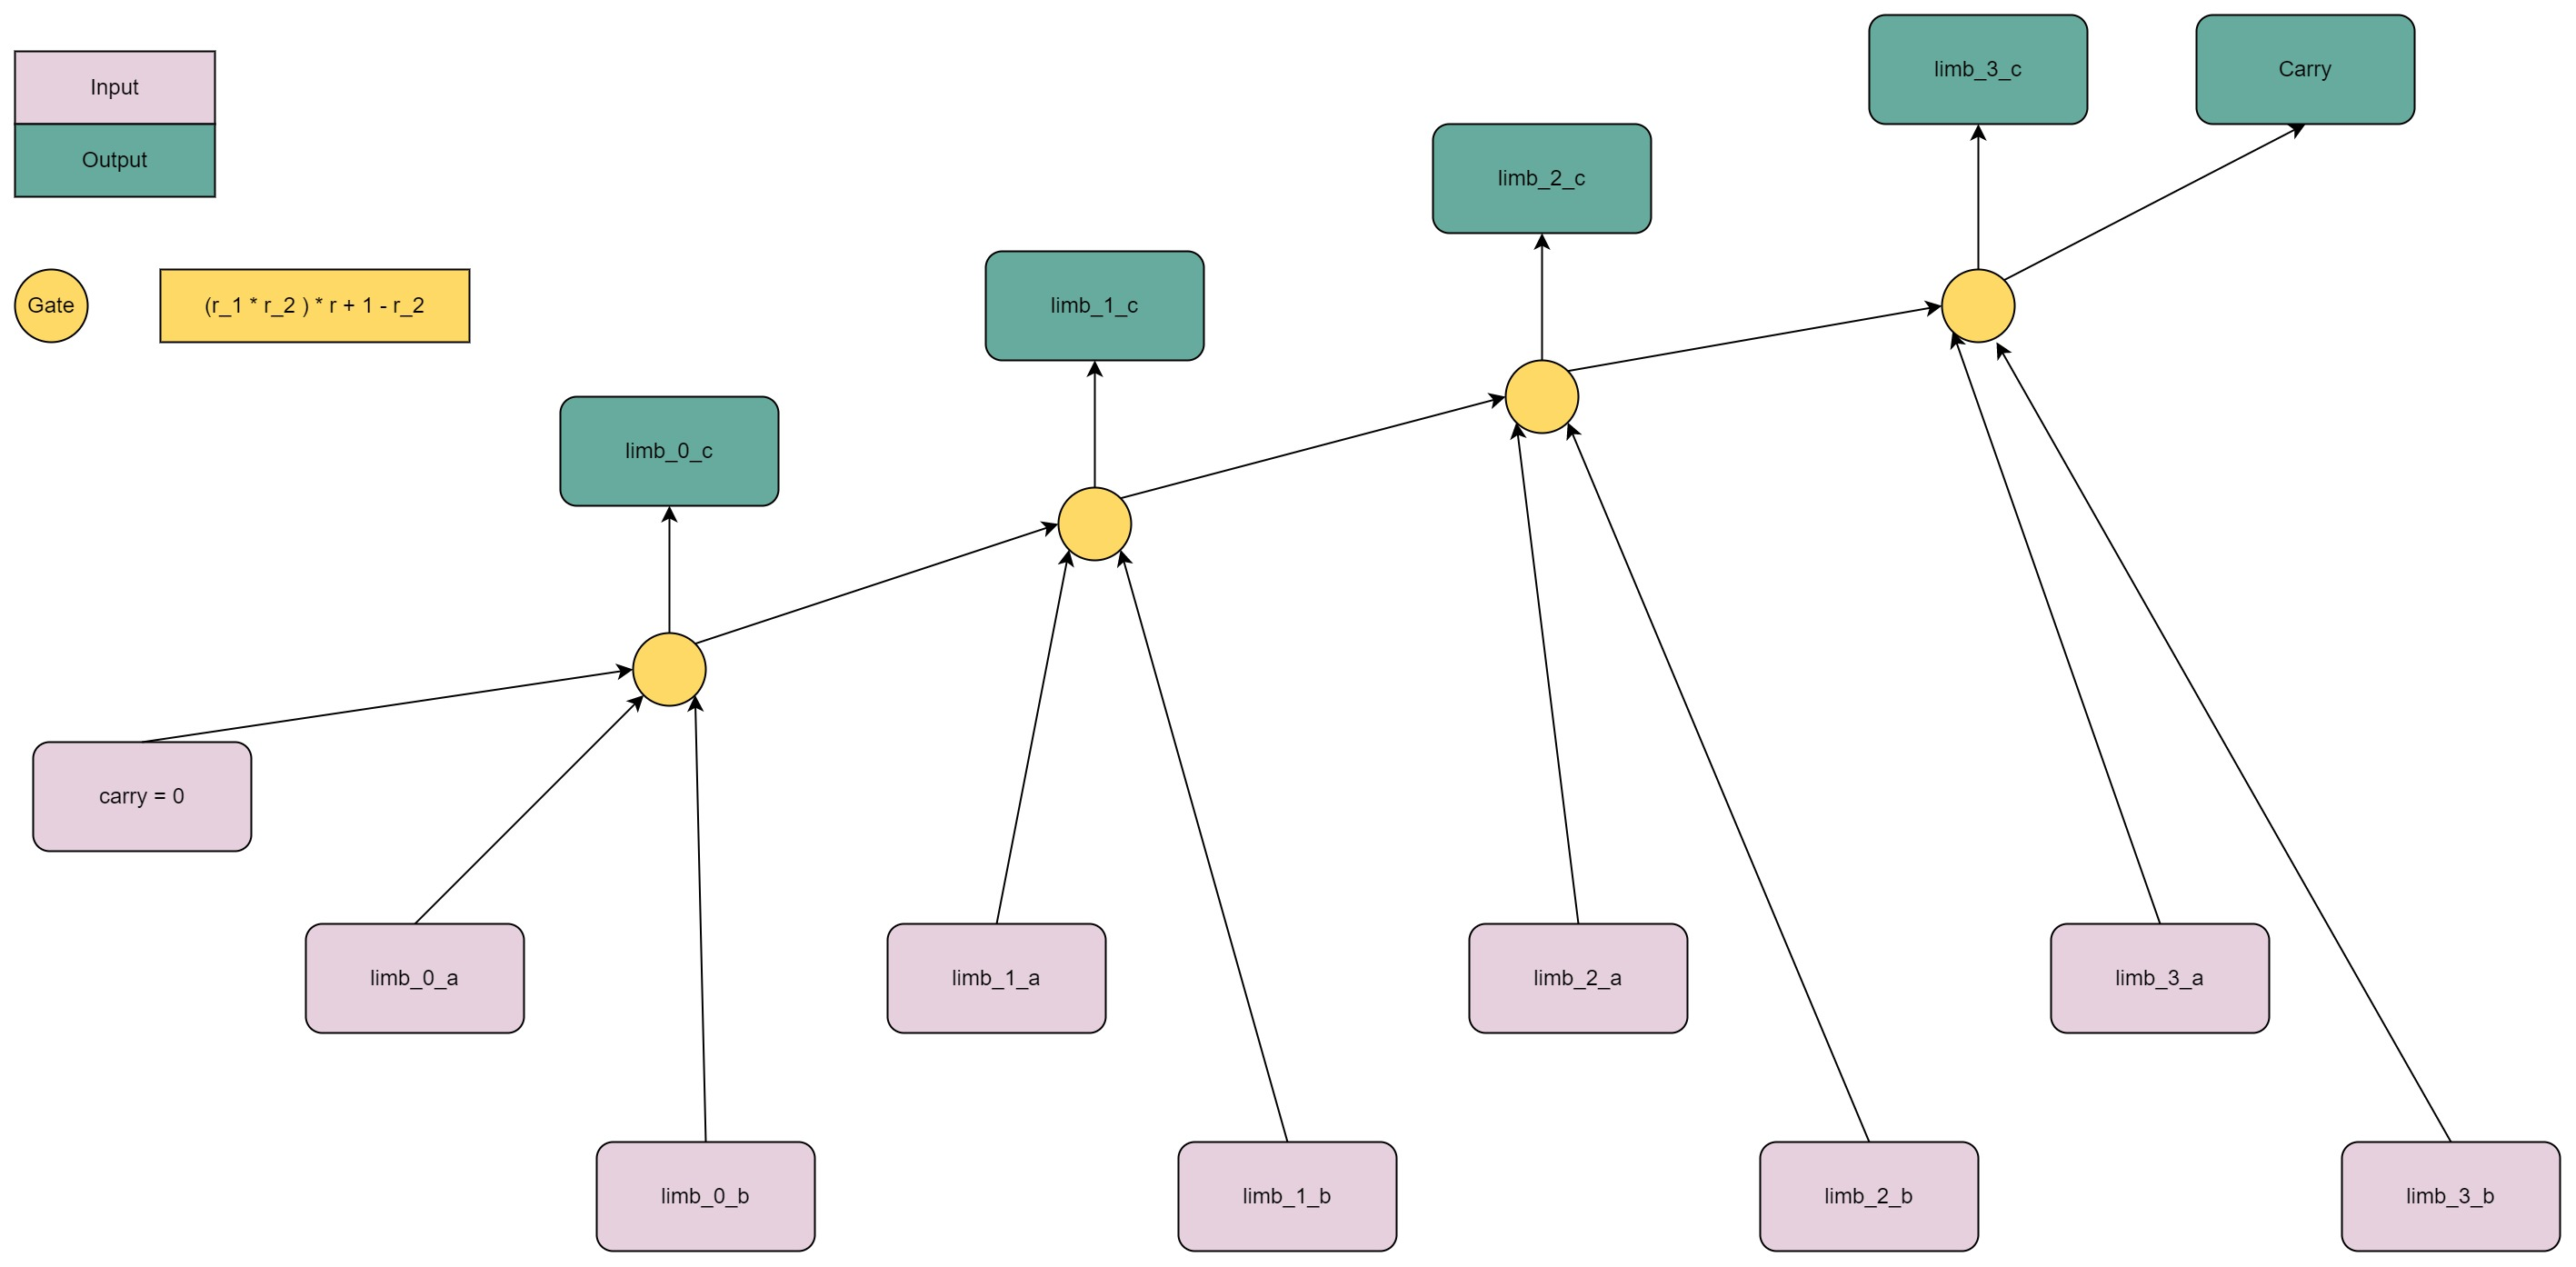
\includegraphics[width=0.8\textwidth]{biguint-add-circuit-layout.jpg}
    \caption{biguint-add circuit layout}
    \label{fig:biguint-add-circuit-layout}
\end{figure}

\Par{Trace layout}
See \figref{fig:biguint-add-trace-layout}.
\begin{figure}[!ht]
    \centering
    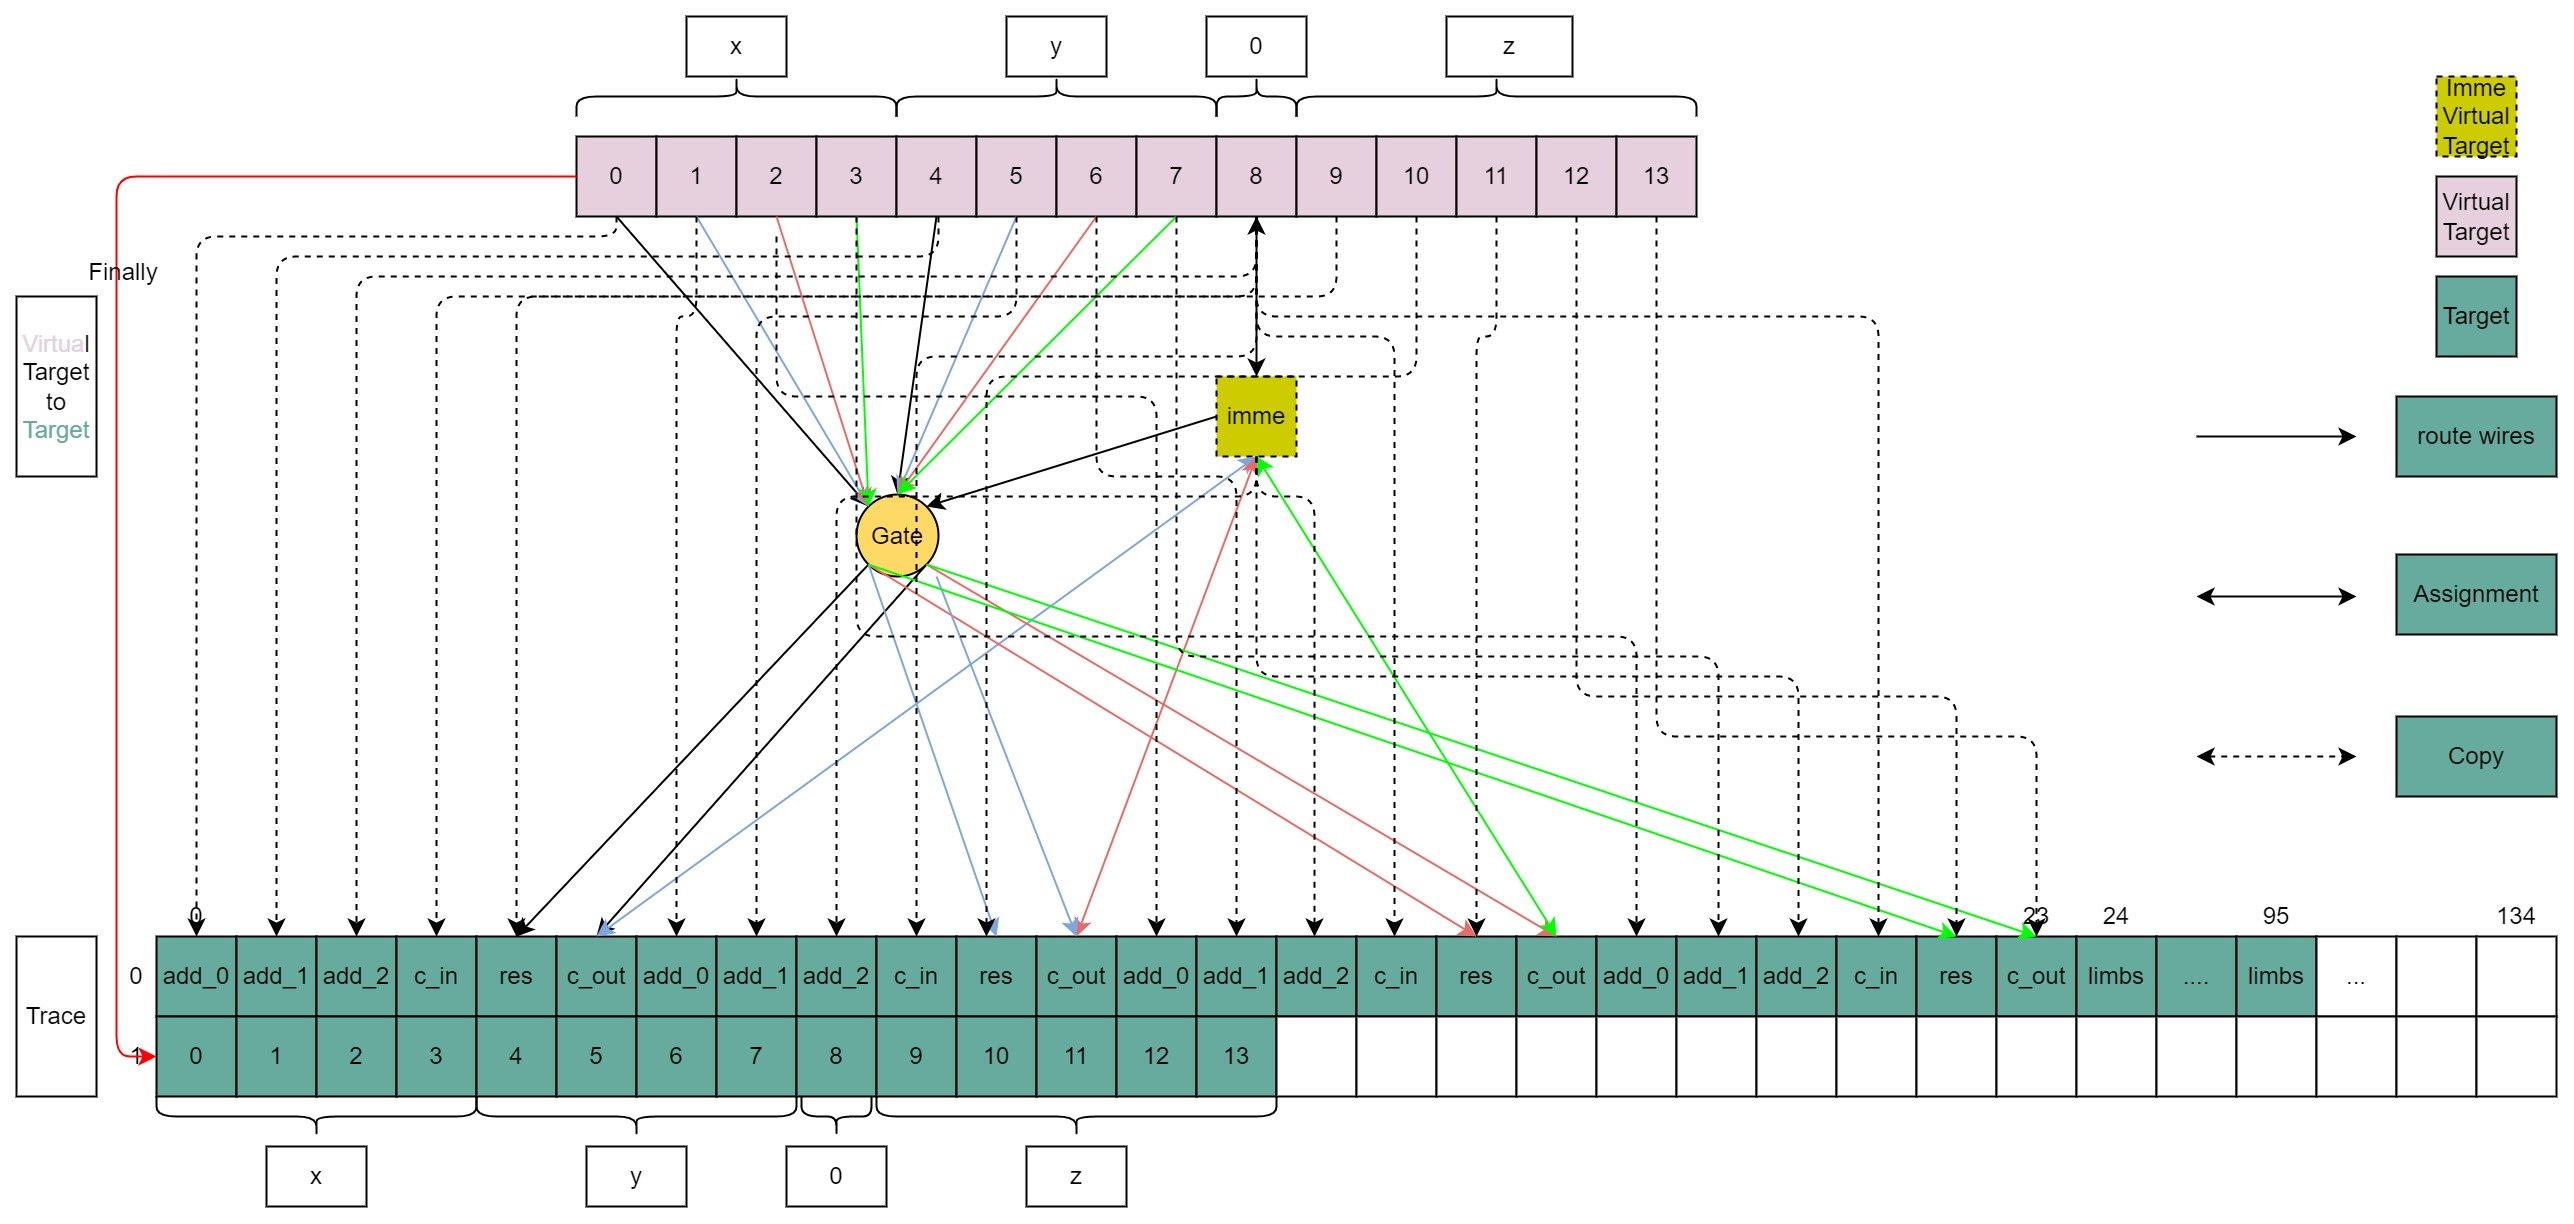
\includegraphics[width=0.8\textwidth]{biguint-add-trace-layout.jpg}
    \caption{biguint-add trace layout}
    \label{fig:biguint-add-trace-layout}
\end{figure}

\Par{Constraints info and costs}
\begin{itemize}
    \item gate type num: 1 (U32AddManyGate)
    \item gate ops num: limbs-num
    \item gate instance num: ceil(limbs-num / gate.ops)
    \item copy-constraints: limbs-num * 4
    \item max-degree: 4 (\verb|1 << limb-bits|)
\end{itemize}

\Par{Questions}
\begin{itemize}
    \item Why not make rangecheck constraint for inputs?
    \item Why not make copy constraint between cur-c-in and last-c-out?
\end{itemize}

    \subsubsection{biguint-sub}

\Par{Target}
Implement the substraction of two biguints.

\Par{Constraints logic}
\begin{itemize}
    \item Equation for gate;
    \item Sumcheck for ouptput;
    \item Rangecheck for limbs.
\end{itemize}

\Par{Circuit layout}
See \figref{fig:biguint-sub-circuit-layout}.
\begin{figure}[!ht]
    \centering
    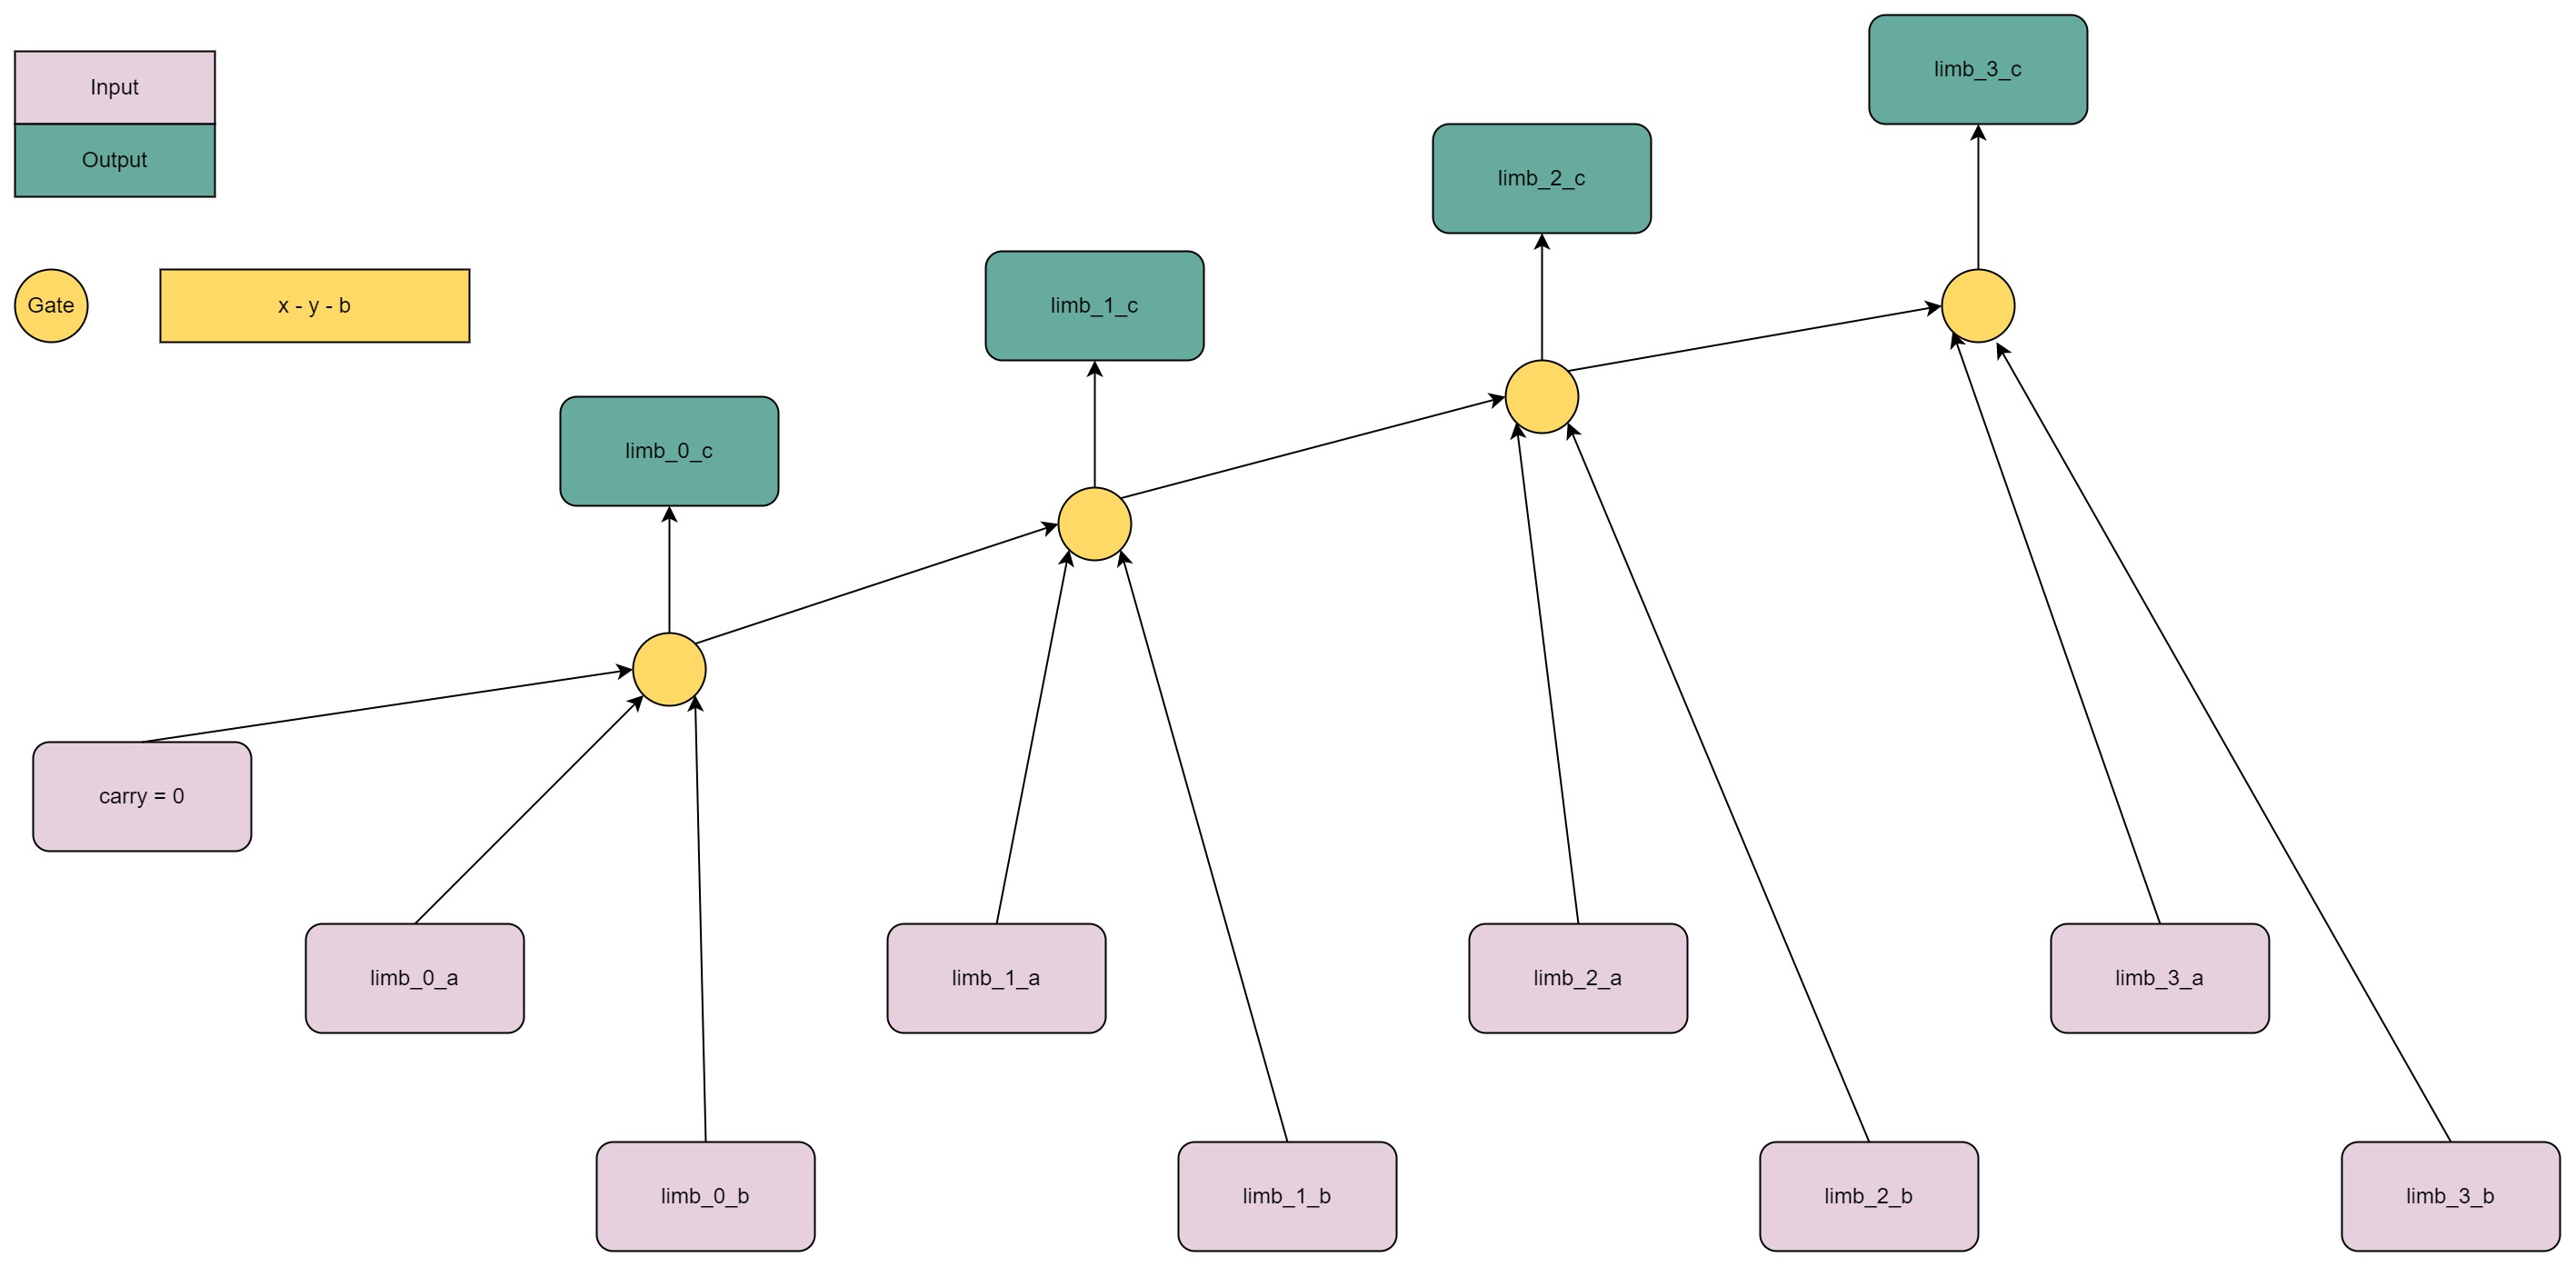
\includegraphics[width=0.8\textwidth]{biguint-sub-circuit-layout.jpg}
    \caption{biguint-sub circuit layout}
    \label{fig:biguint-sub-circuit-layout}
\end{figure}

\Par{Trace layout}
See \figref{fig:biguint-sub-trace-layout}.
\begin{figure}[!ht]
    \centering
    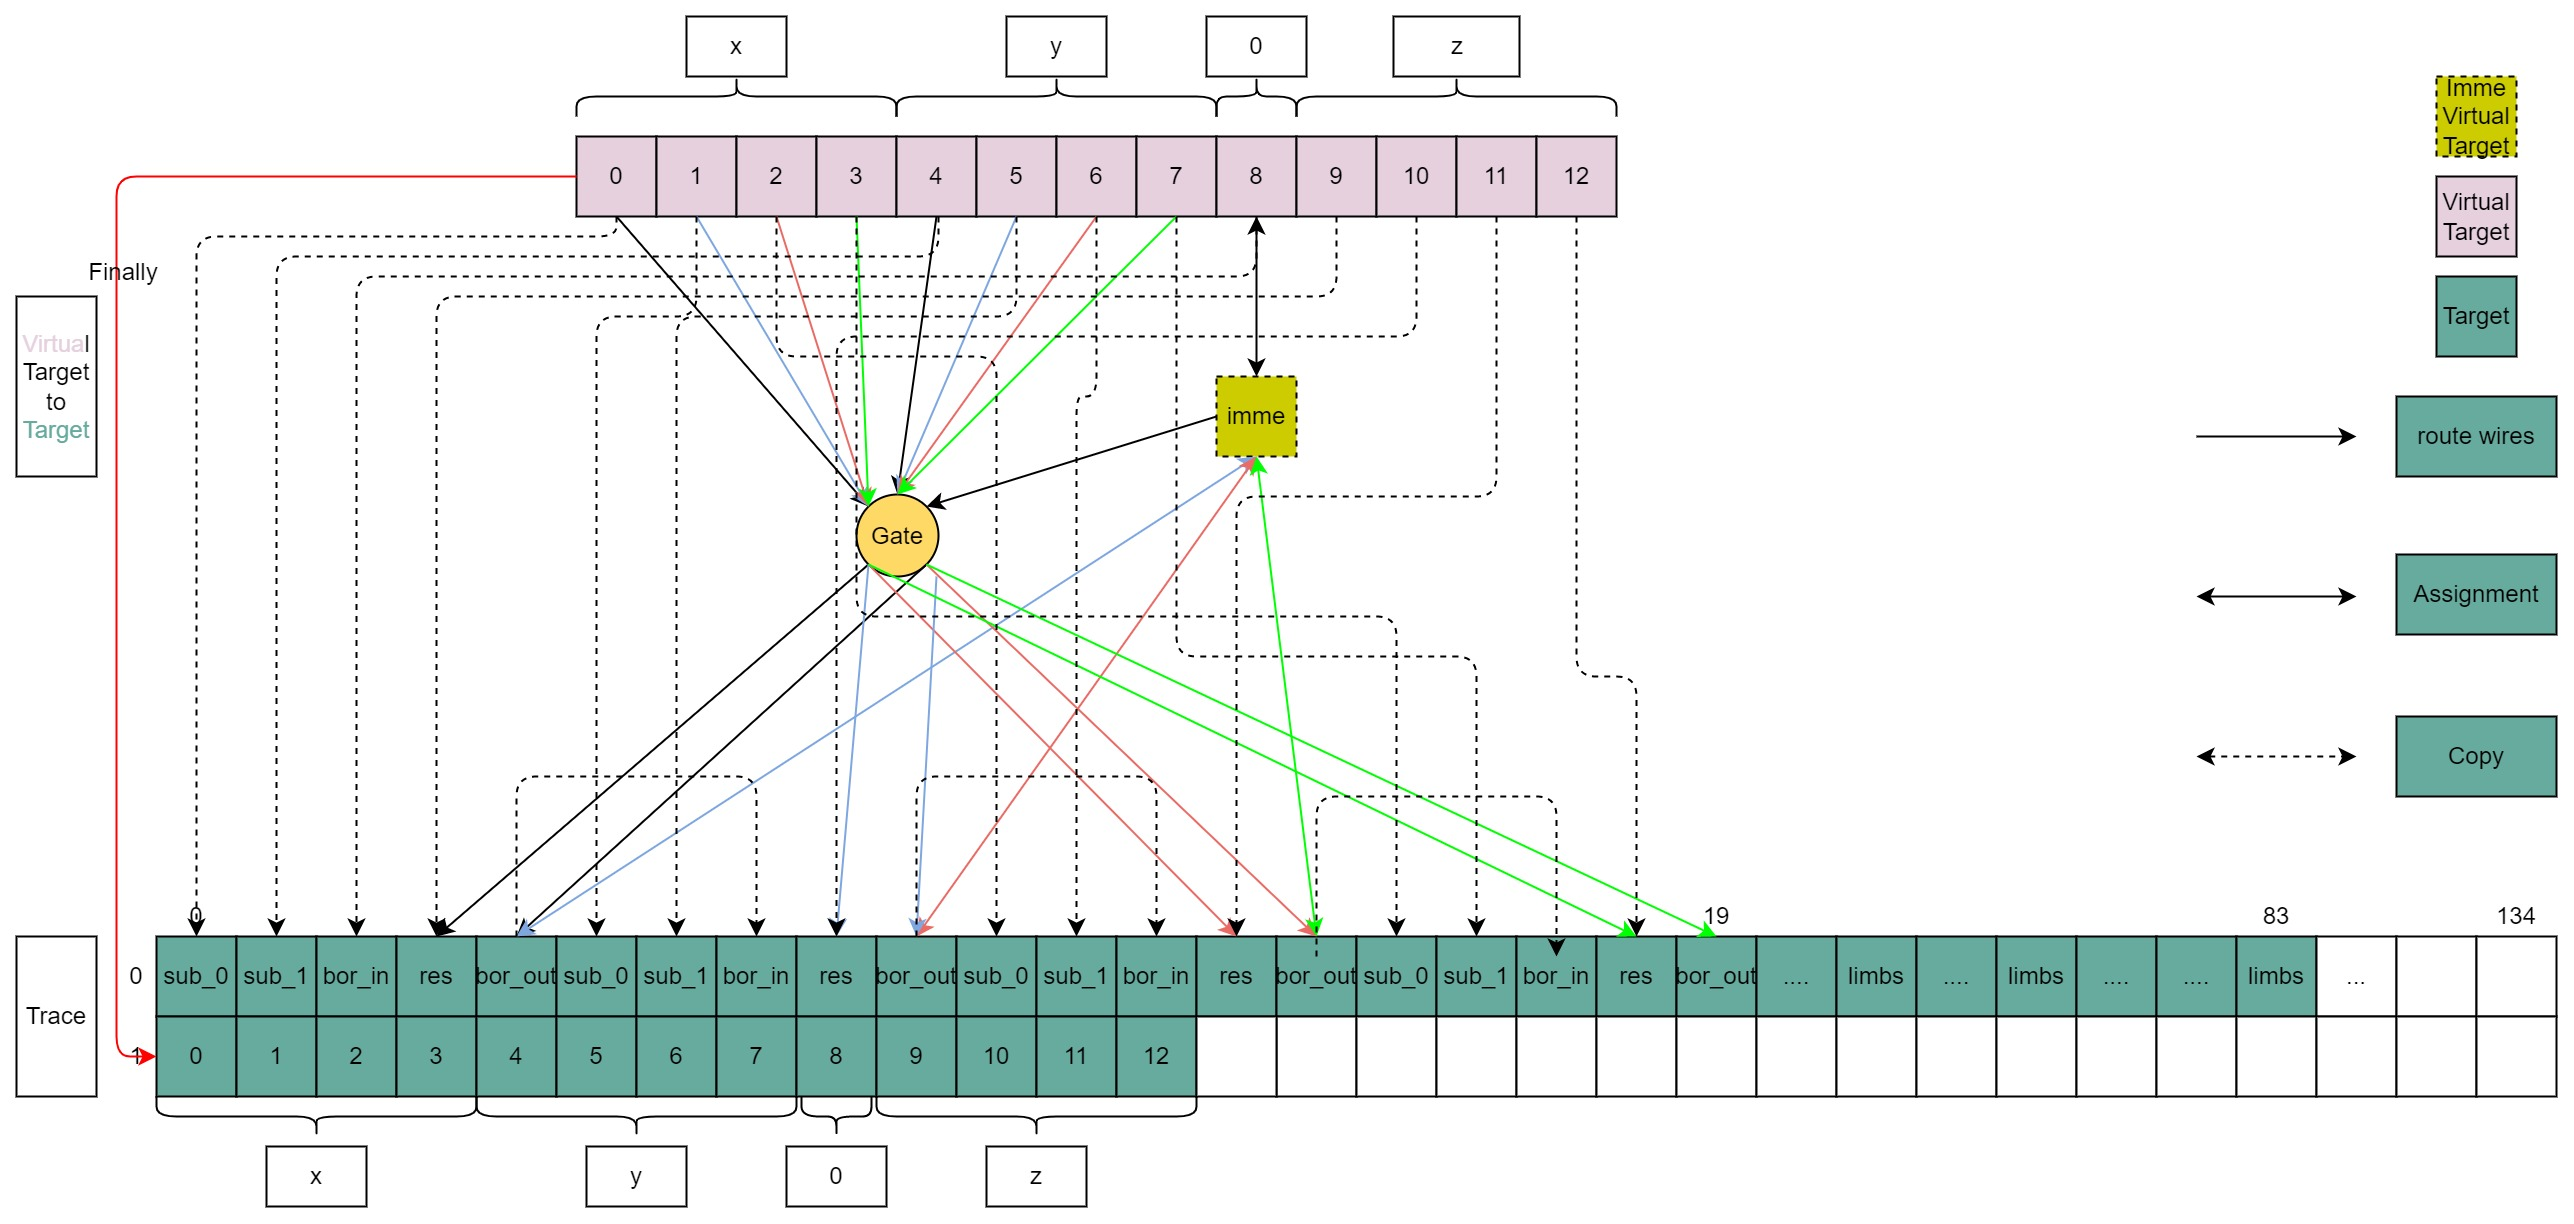
\includegraphics[width=0.8\textwidth]{biguint-sub-trace-layout.jpg}
    \caption{biguint-sub trace layout}
    \label{fig:biguint-sub-trace-layout}
\end{figure}

\Par{Constraints info and costs}
\begin{itemize}
    \item constraints-num: $6 \times (3 + 32 / 2) = 114$
    \item copy-constraints: $16$
    \item max-degree: $4$
    \item wires-num: $6 \times (5 + 16) = 126$
\end{itemize}

\Par{Questions}
\begin{itemize}
    \item Why not make rangecheck constraint for inputs?
    \item Could try to use the same constraint with add-gate.
\end{itemize}

    \subsubsection{biguint-mul}

\Par{Target}
Implement the multiplication of two biguints.

\Par{Constraints logic}
\begin{itemize}
    \item Compute mul-factors first, use U32ArithmeticGate;
    \item Add mul-factors from low bits, use U32AddManyGate.
\end{itemize}

\Par{Process layout}
See \figref{fig:biguint-mul-layout}
\begin{figure}[!ht]
    \centering
    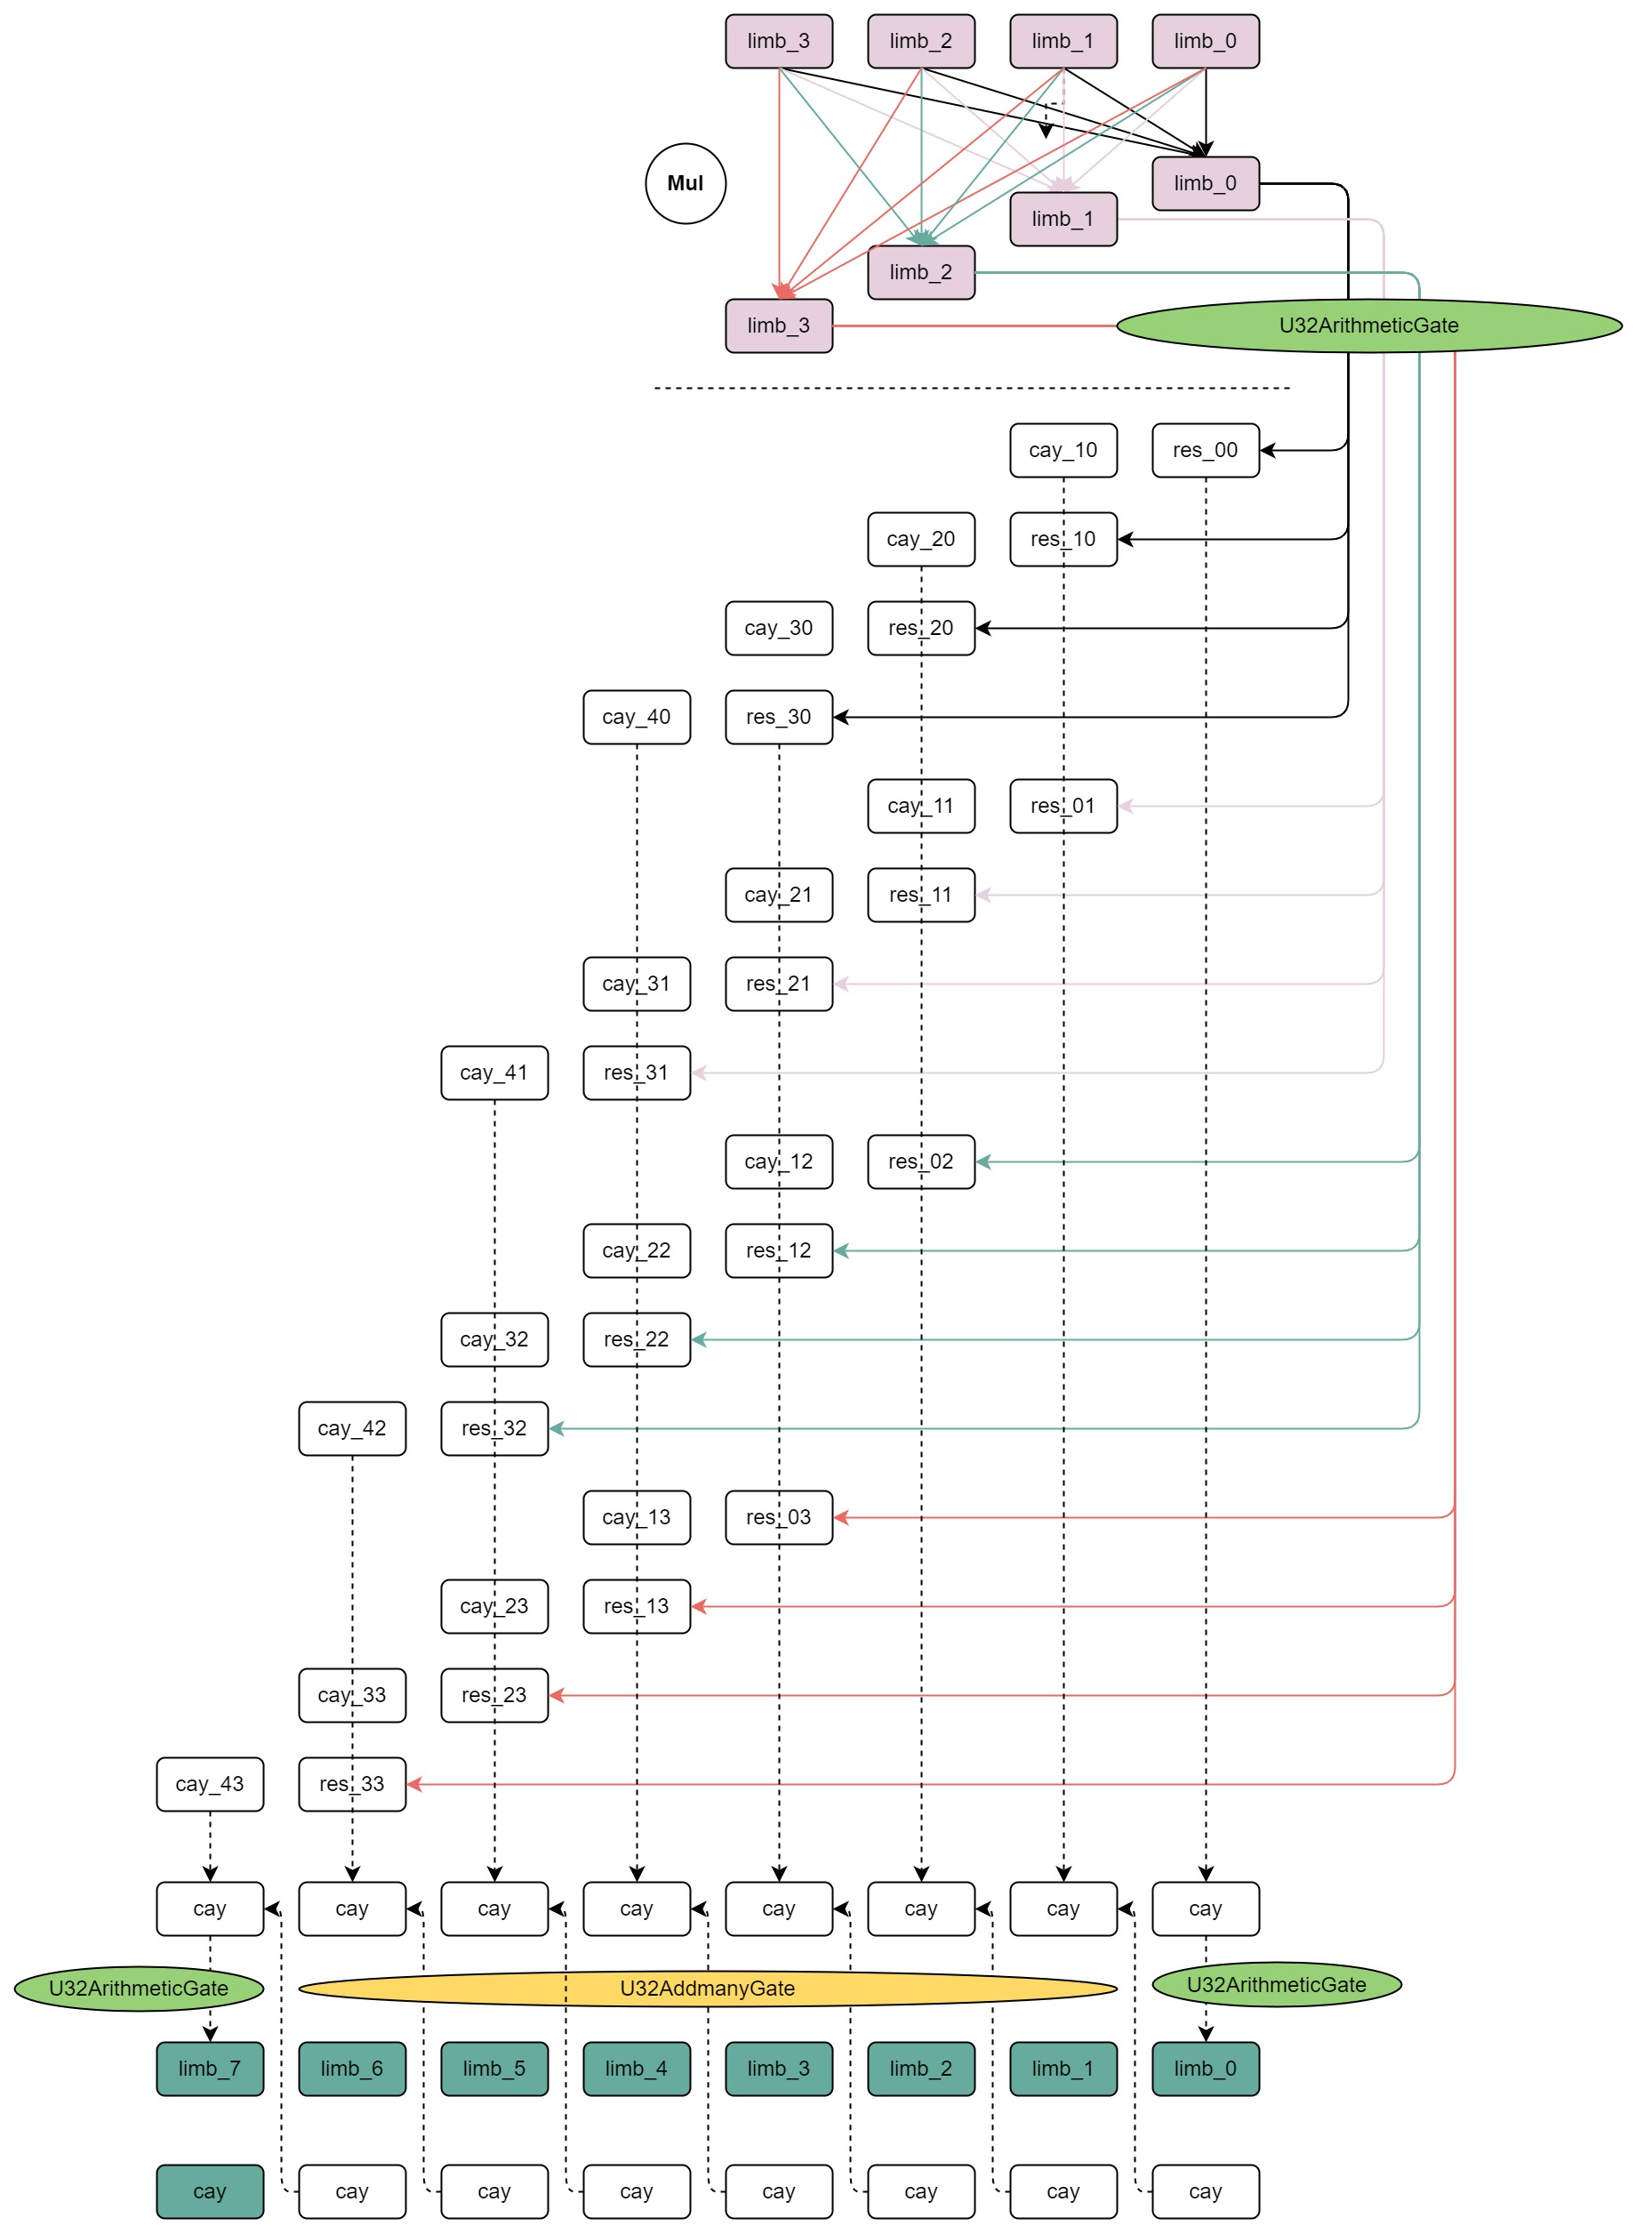
\includegraphics[width=0.8\textwidth]{biguint-mul-layout.jpg}
    \caption{biguint-mul layout}
    \label{fig:biguint-mul-layout}
\end{figure}

\Par{Constraints info and costs}
\begin{itemize}
    \item Gate type num: 4 (U32ArithmeticGate, U32AddManyGate(num-addends: 4), U32AddManyGate(num-addends: 6), U32AddManyGate(num-addends: 8))
    \item Gate instance num: 9
    \item U32ArithmeticGate num: 6
    \item U32AddManyGate num: 3
    \item copy-constraints: $18 \times 3 + (4 + 6 + 8) \times 2 + 9 = 99$
    \item max-degree: 4
\end{itemize}

    \section{biguint-div}
\label{biguint-div}

Note that div-rem has the same constraints logic with div

\begin{enumerate}
    \item target
        \begin{itemize}
            \item implement the division of two biguints
        \end{itemize}
    \item constraints-logic
        \begin{itemize}
            \item not implement div-algrithem directly
            \item use nondeterministic feature to check div-logic
            \item check div * b + rem = a
            \item check rem < b
        \end{itemize}
    \item div-process layout
        \begin{figure}[!ht]
            \centering
            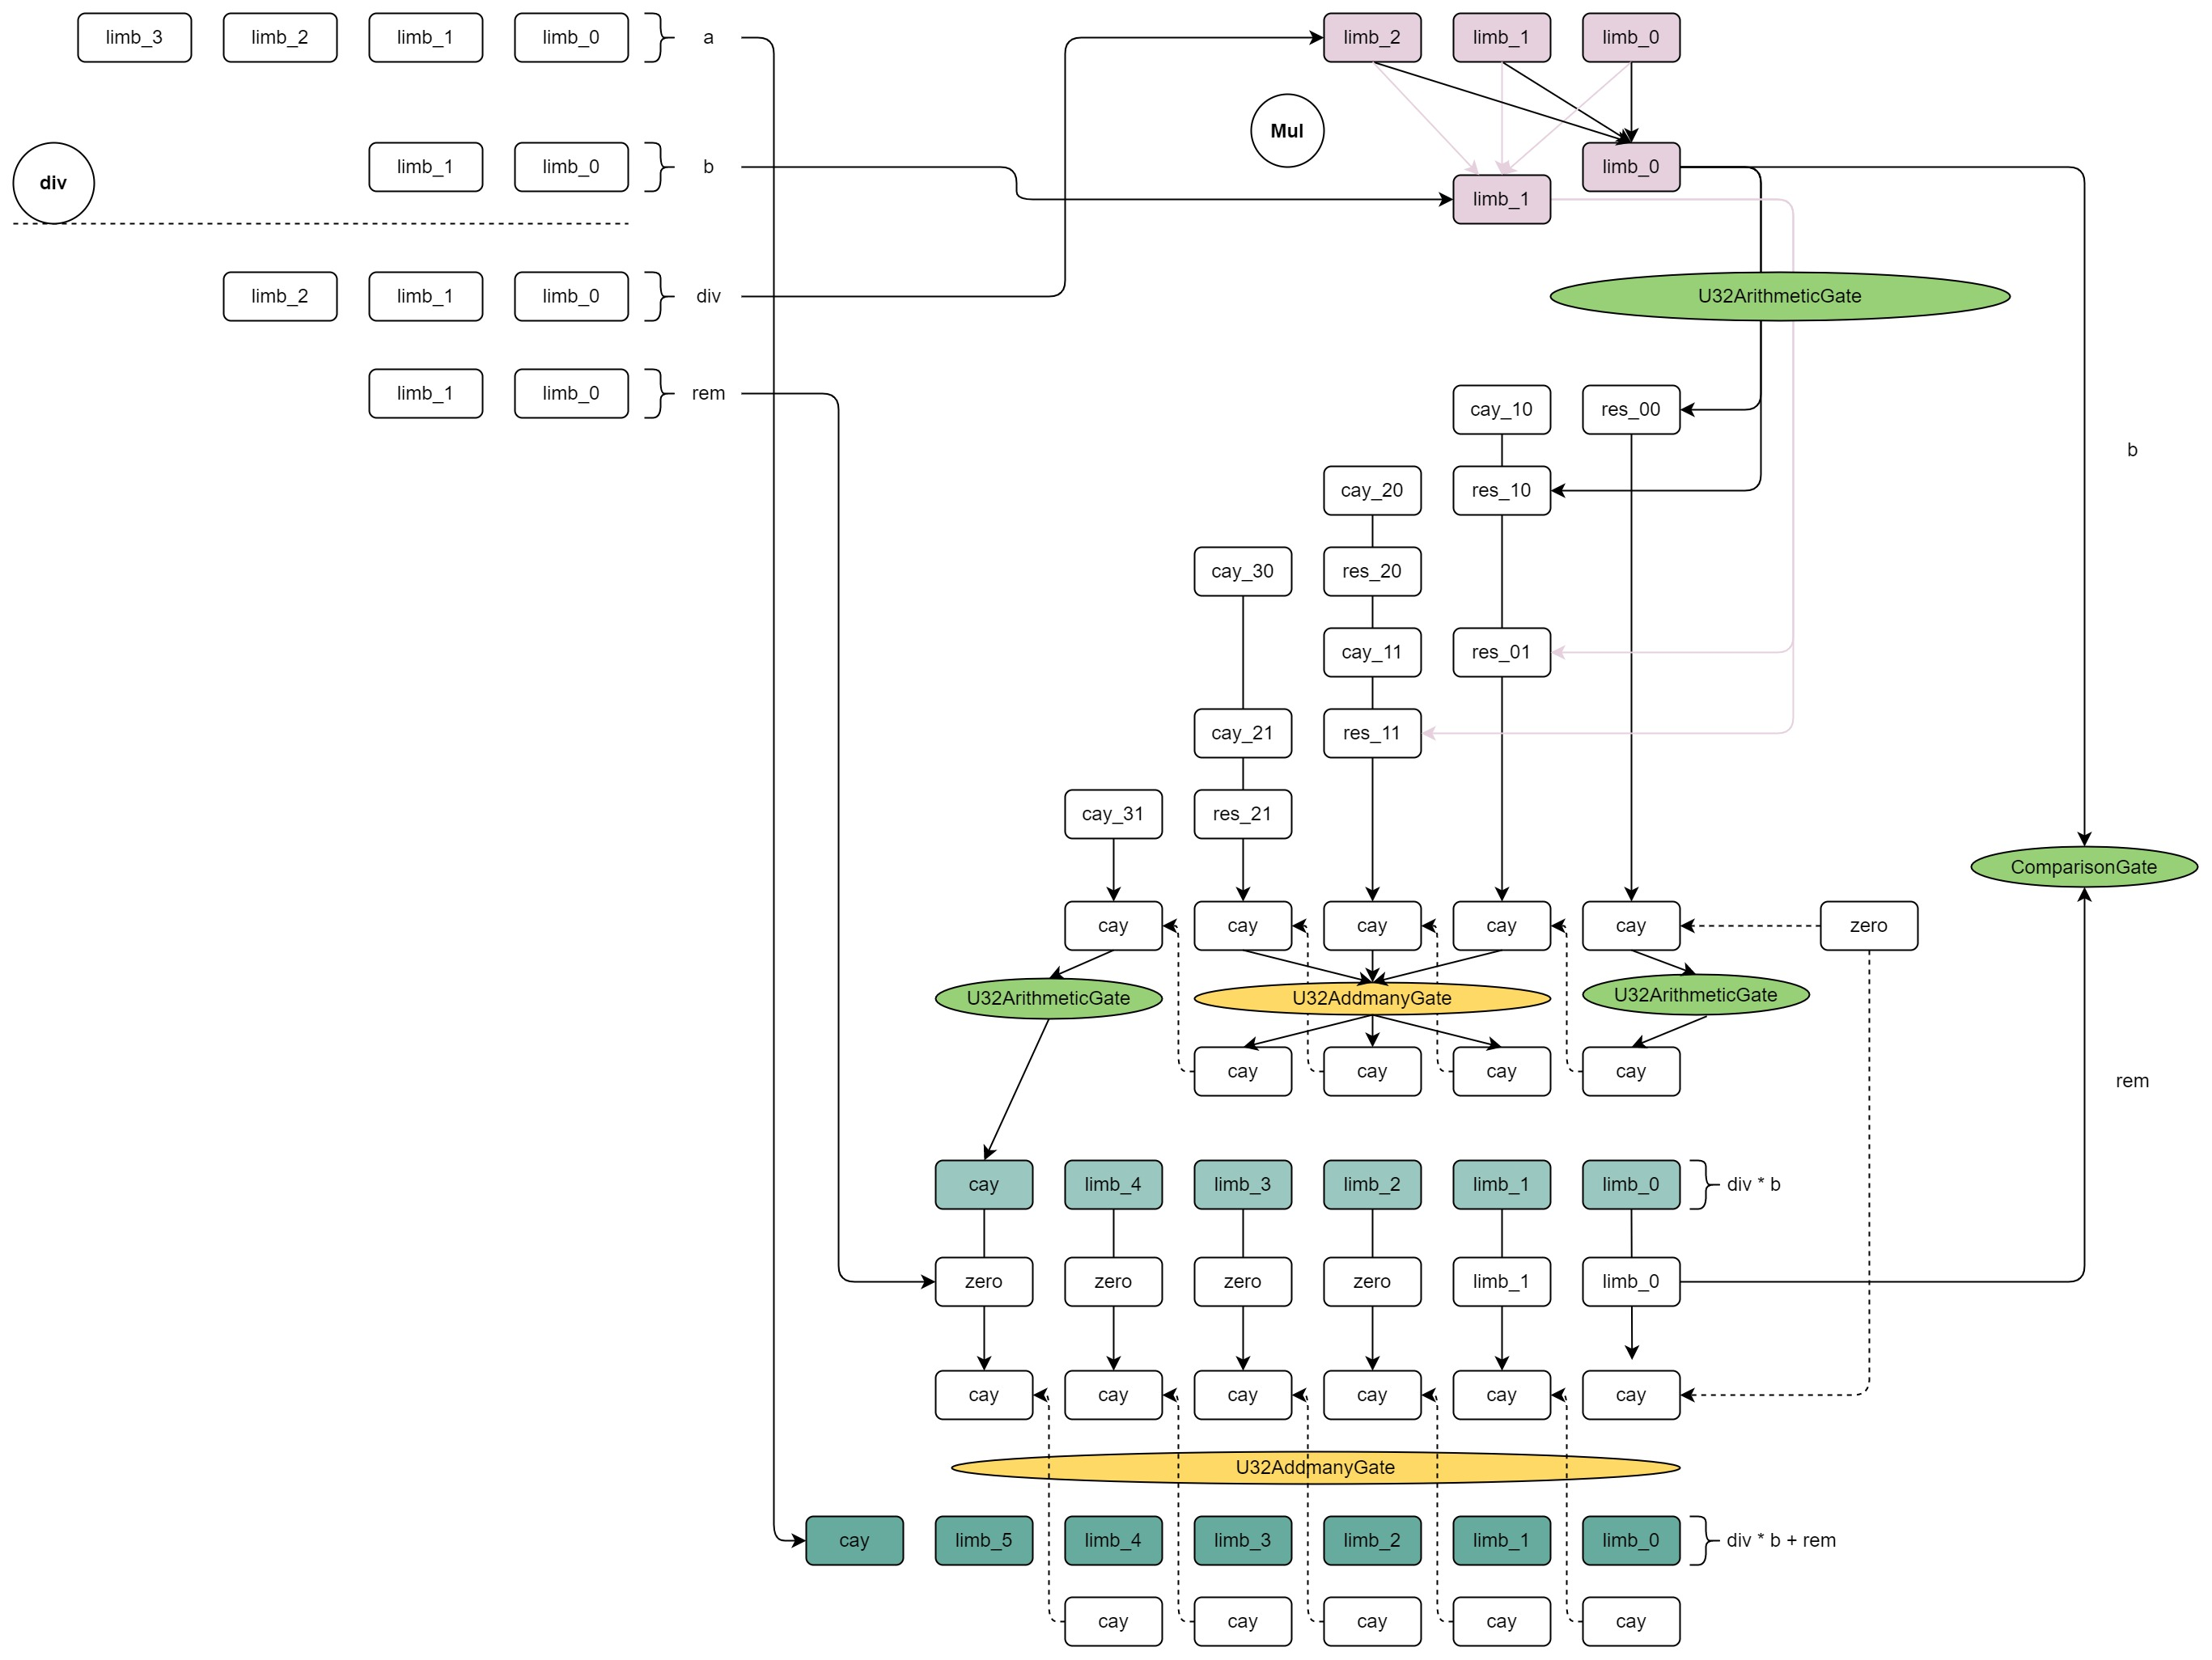
\includegraphics[width=0.8\textwidth]{biguint-div-layout.jpg}
            \caption{biguint-div layout.jpg}
            \label{fig:biguint-div-layout.jpg}
        \end{figure}
    
    \item constraints-info and costs
        \begin{itemize}
            \item Gate type num: 5(U32ArithmeticGate, U32AddManyGate(num-addends: 3), U32AddManyGate(num-addends: 4), ComparisionGate, ArithmeticGate)
            \item Gate instance num: 3 + 3 + 4 + 3 = 13 
            \item U32ArithmeticGate num: 3
            \item U32AddManyGate num: 3
            \item ComparisionGate num: 4
            \item ArithmeticGate num: 3
            \item copy-constraints: 3 * 8 + 4 + 5 + 4 + 4 * 6 + 7 + 1 + 26 + 5 = 100 
            \item max-degree: 4
        \end{itemize}

\end{enumerate}
    \subsubsection{biguint-cmp}

\Par{Target}
Implement the comparison of two biguints.

\Par{Constraints logic}
\begin{itemize}
    \item Split the input to many limbs, such that: \verb|limbs_num = bits / chunks|;
    \item Execute comparison for low bits limbs;
    \item Ensure that the result is determined by the highest limbs which are not equal.
\end{itemize}

\Par{Process layout}
See \figref{fig:biguint-cmp-layout}.
\begin{figure}[!ht]
    \centering
    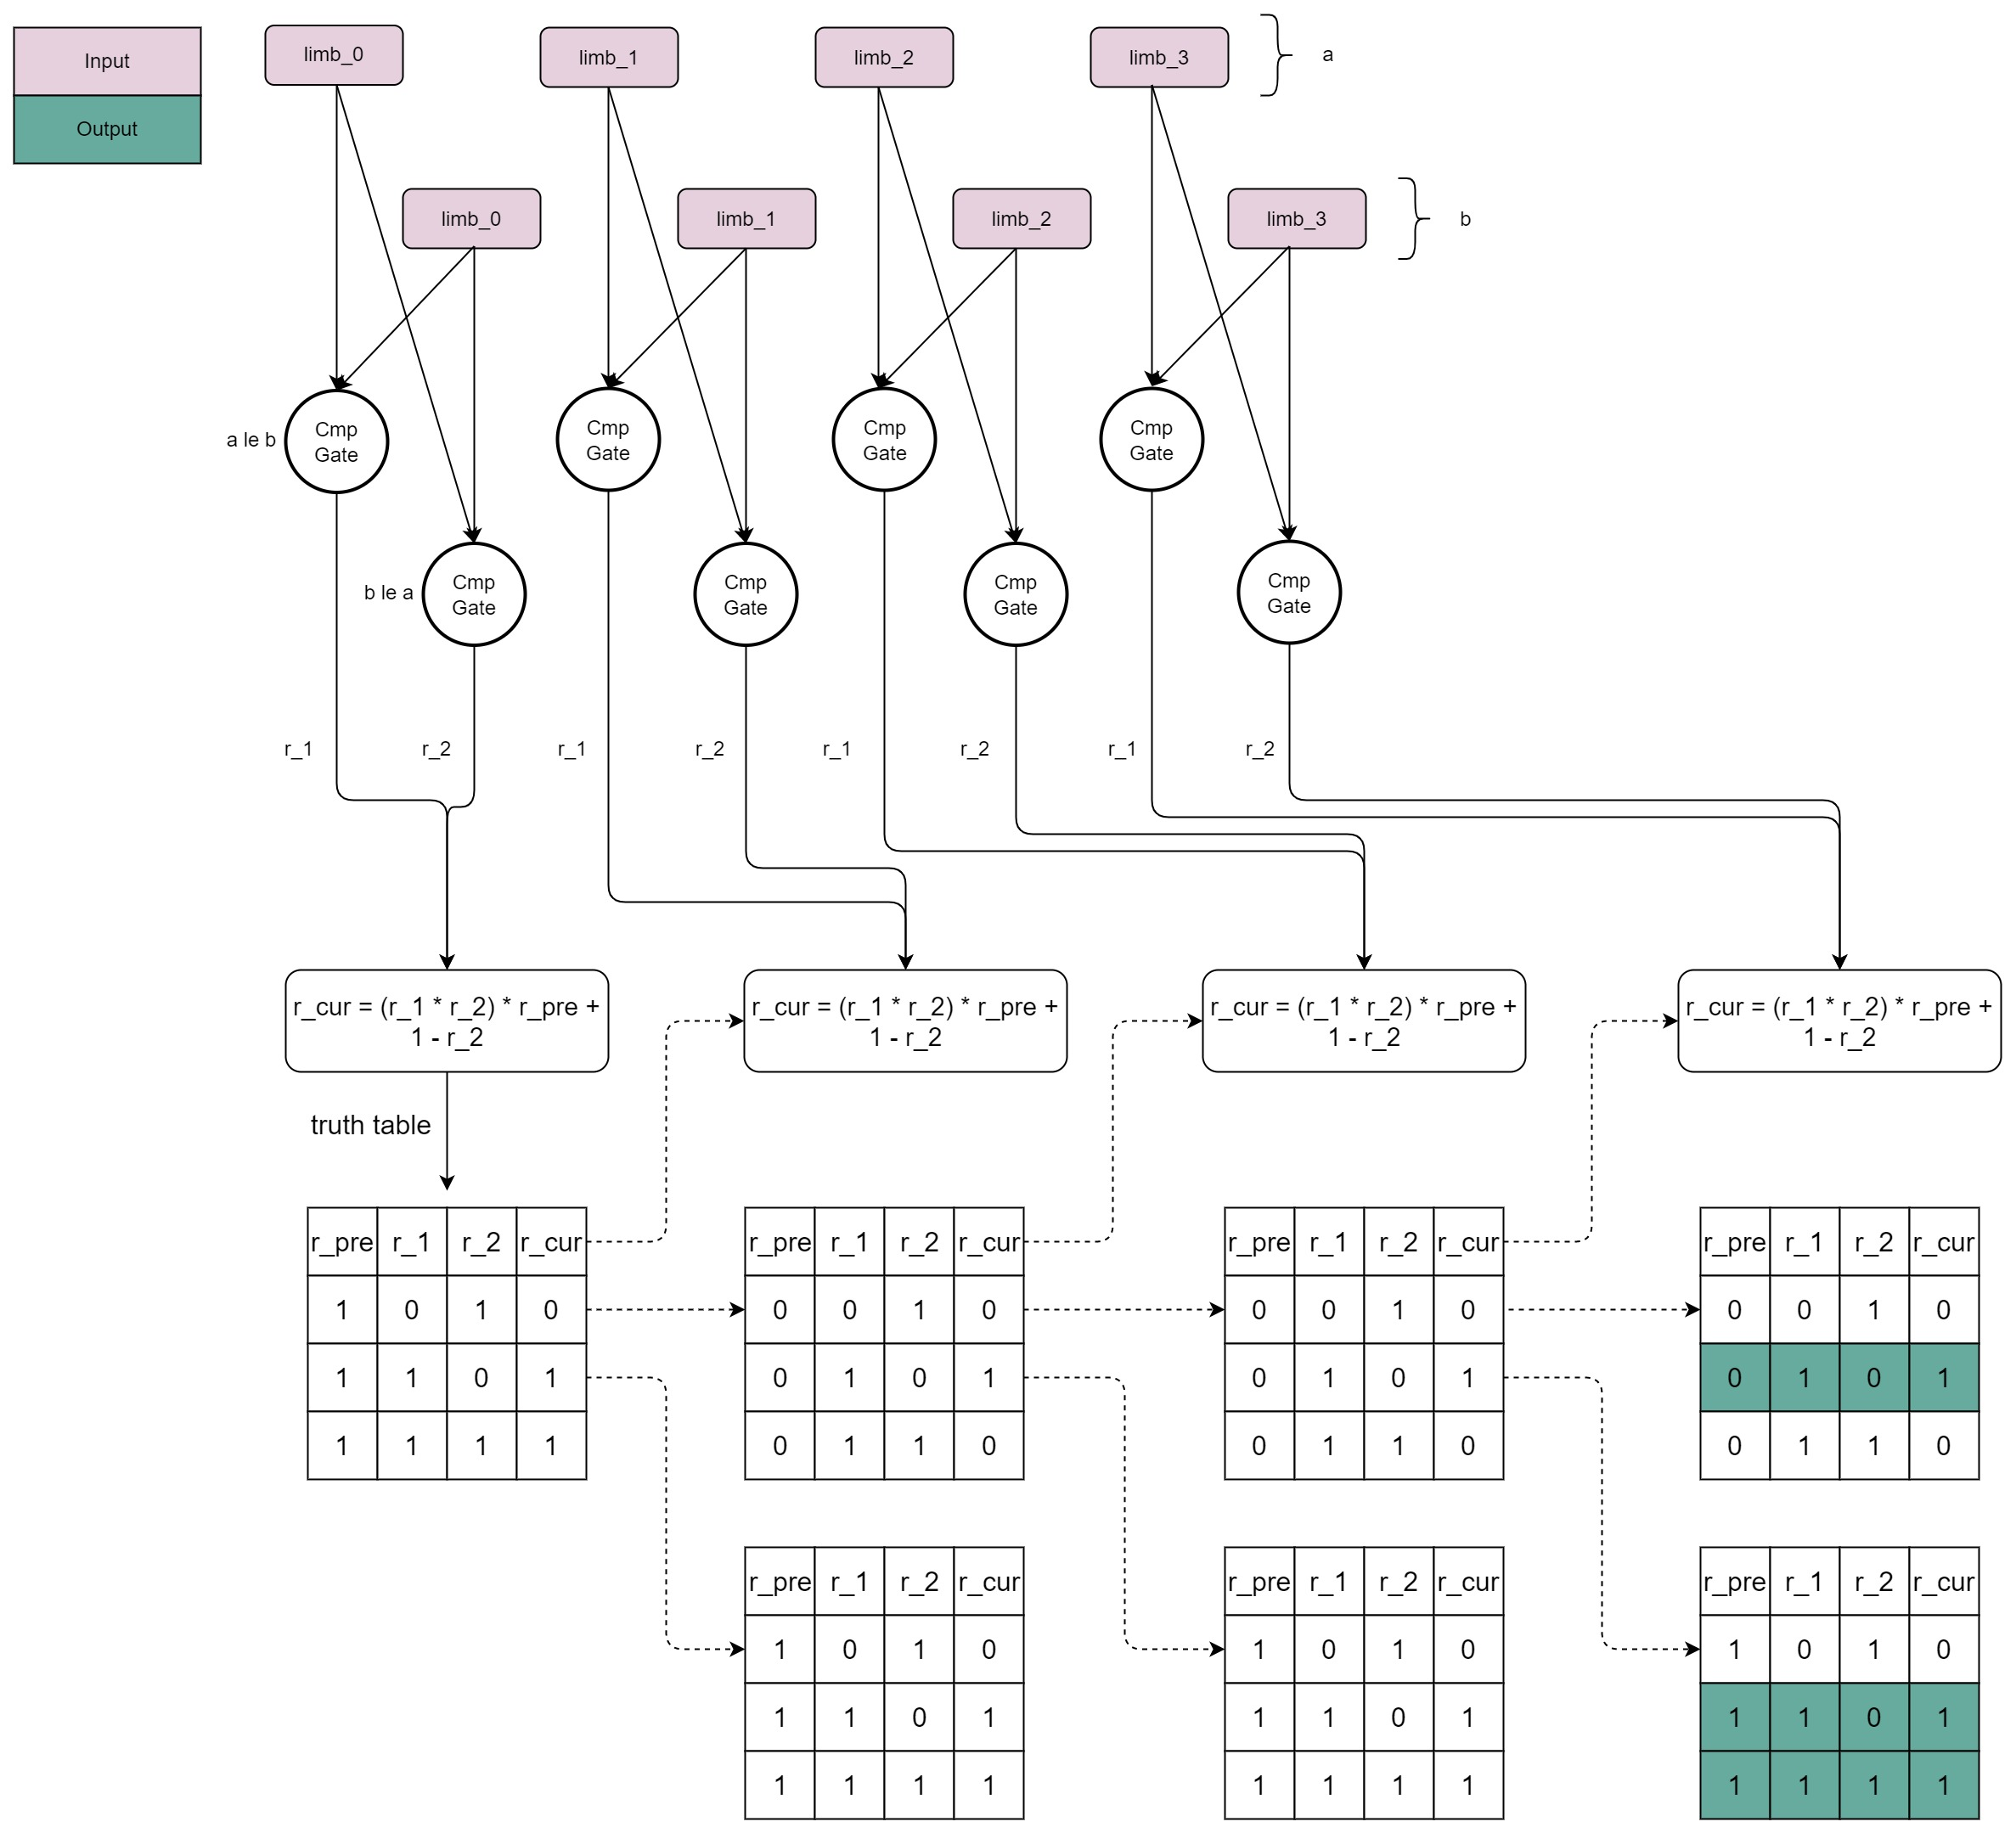
\includegraphics[width=0.8\textwidth]{biguint-cmp-layout.jpg}
    \caption{biguint-cmp layout}
    \label{fig:biguint-cmp-layout}
\end{figure}

\Par{Circuit layout}
See \figref{fig:biguint-cmp-circuit-layout}.
\begin{figure}[!ht]
    \centering
    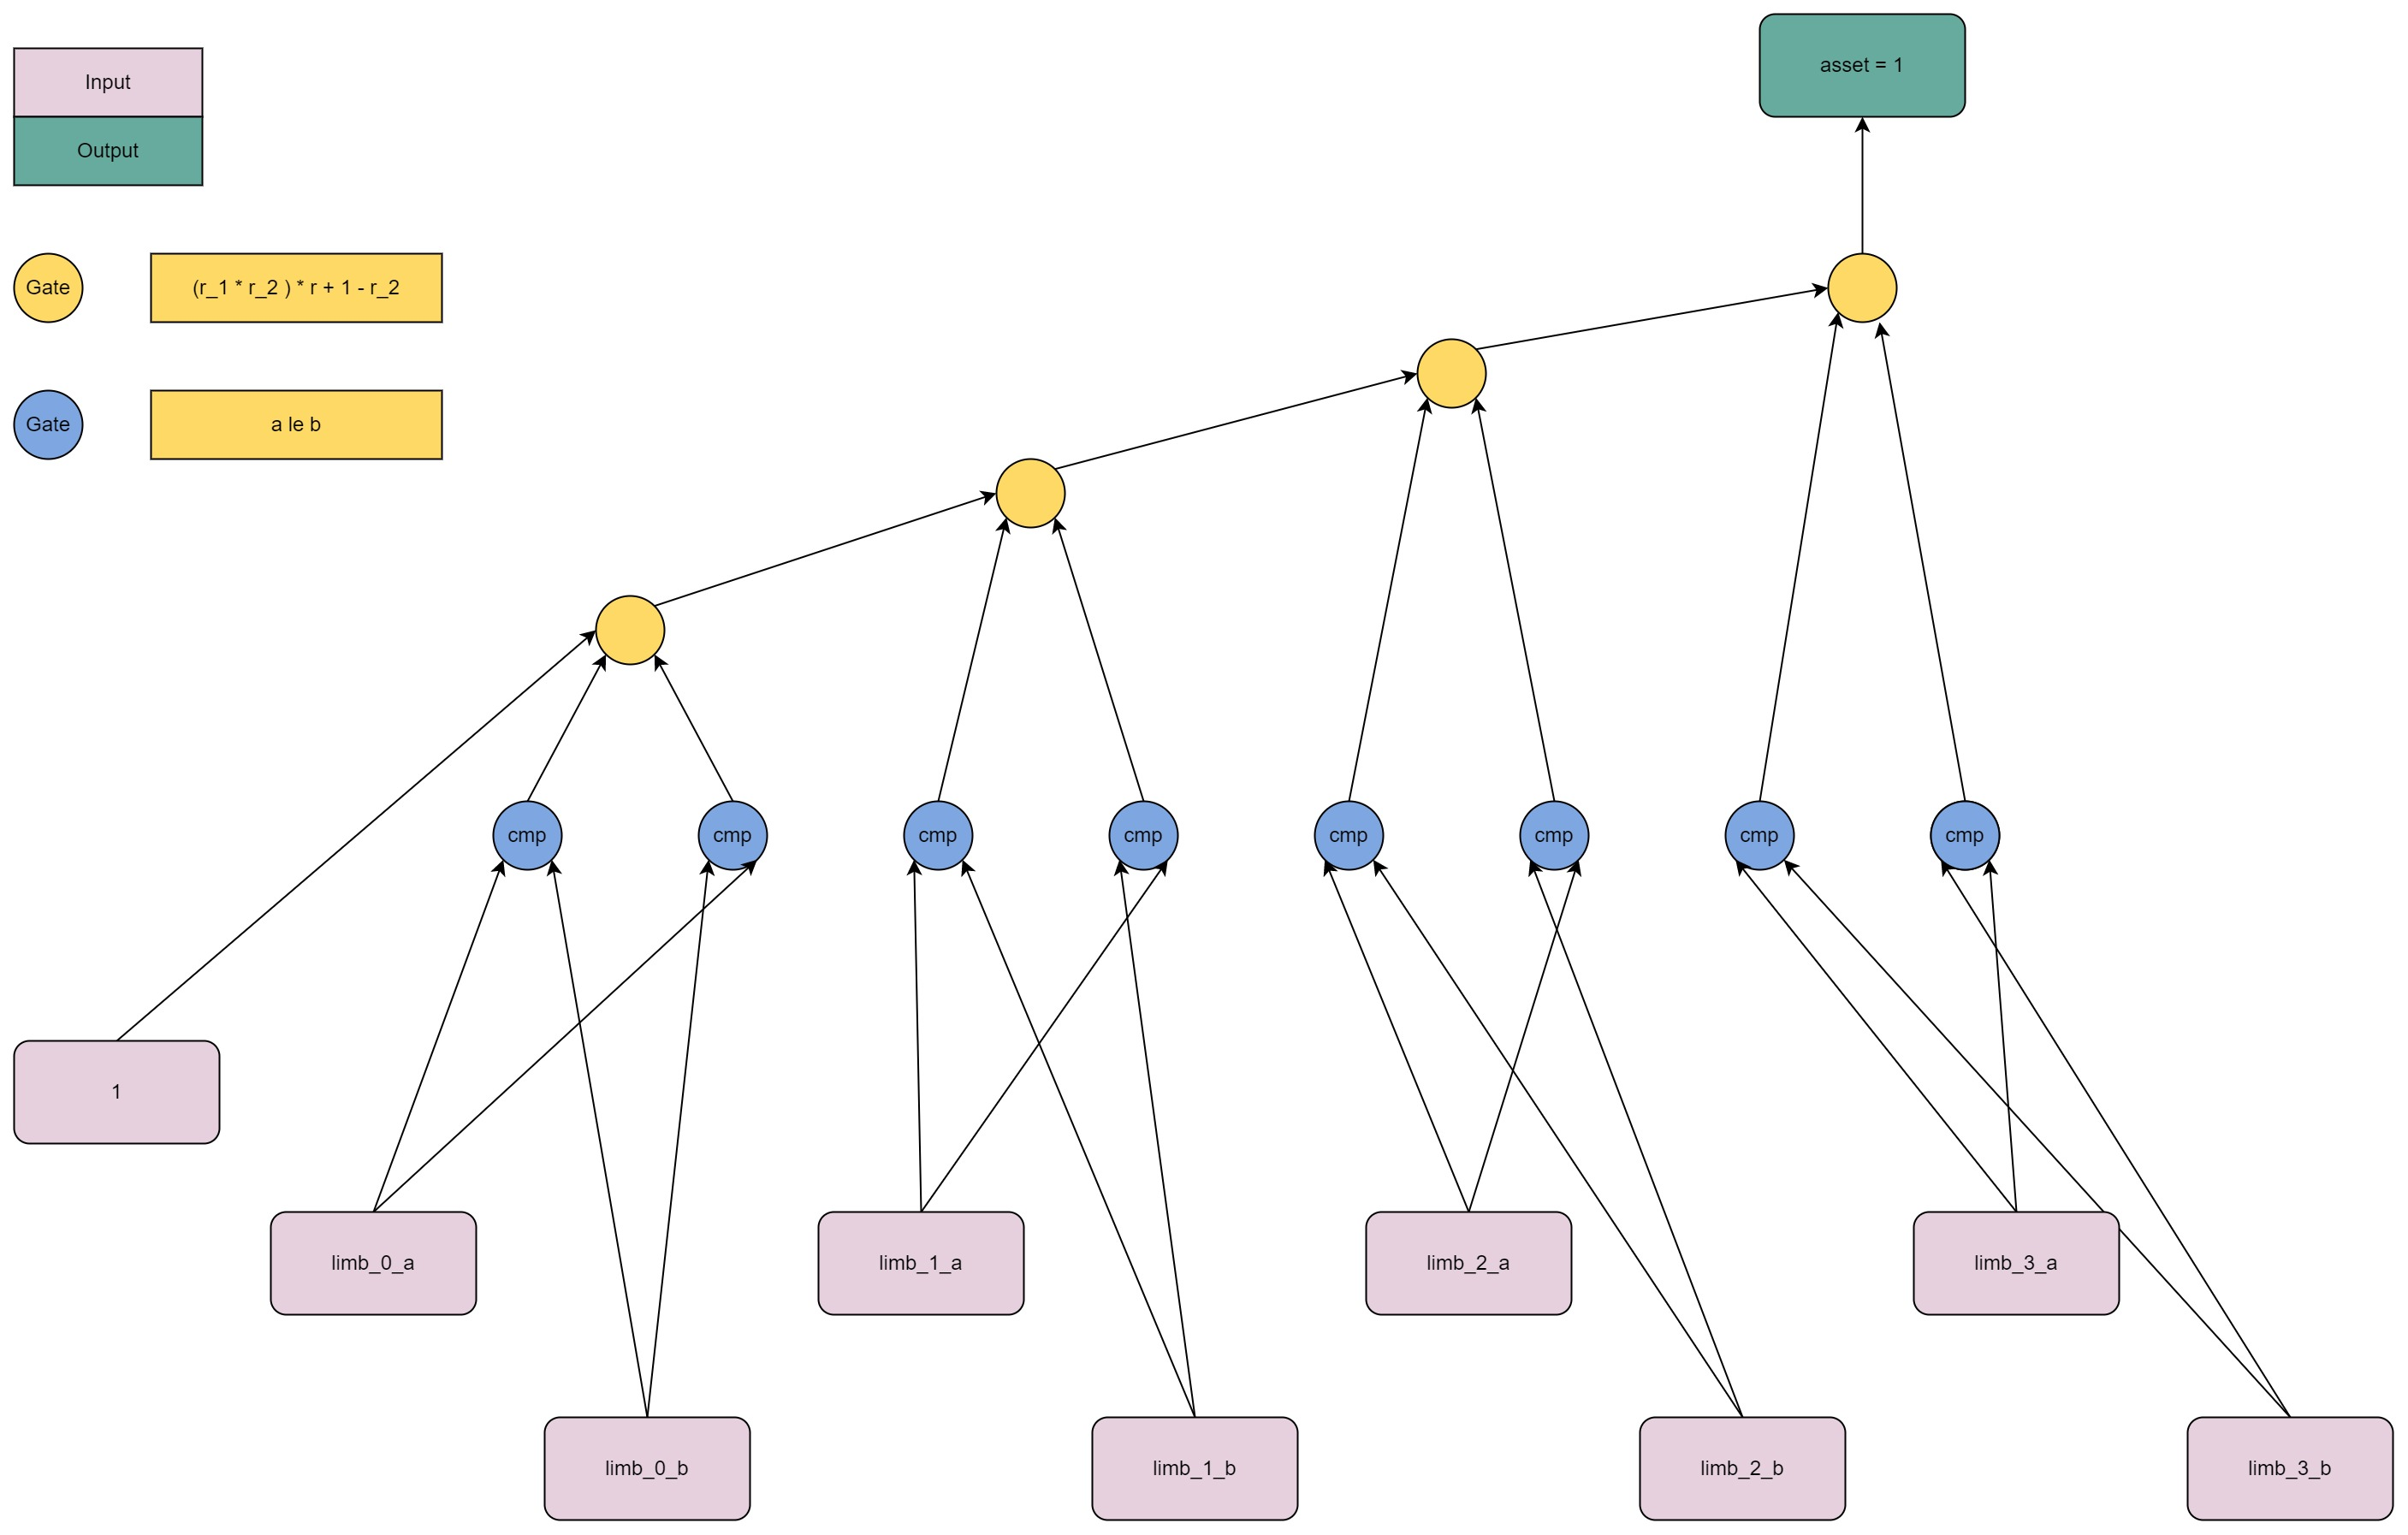
\includegraphics[width=0.8\textwidth]{biguint-cmp-circuit-layout.jpg}
    \caption{biguint-cmp circuit layout}
    \label{fig:biguint-cmp-circuit-layout}
\end{figure}

\Par{Constraints info and costs}
\begin{itemize}
    \item Gate type num: 2 (ComparisionGate, ArithmeticGate)
    \item Gate instance num: $4 \times 2 + 3 = 11$
    \item ComparisionGate num: 8
    \item ArithmeticGate num: 3
    \item copy-constraints: $(4 + 9) \times 4 + 1 = 53$
    \item max-degree: 4
\end{itemize}

    \subsubsection{nonnative-add}
\label{nonnative-add}

\begin{enumerate}
    \item target
        check the additional relation among three nonnative target objects.
    \item constraints-logic
        \begin{itemize}
            \item check equation for gadget,  a + b = c + modular * overflow
            \item check that "c lt modular"
        \end{itemize}
    \item nonnative-add process layout
        \begin{figure}[!ht]
            \centering
            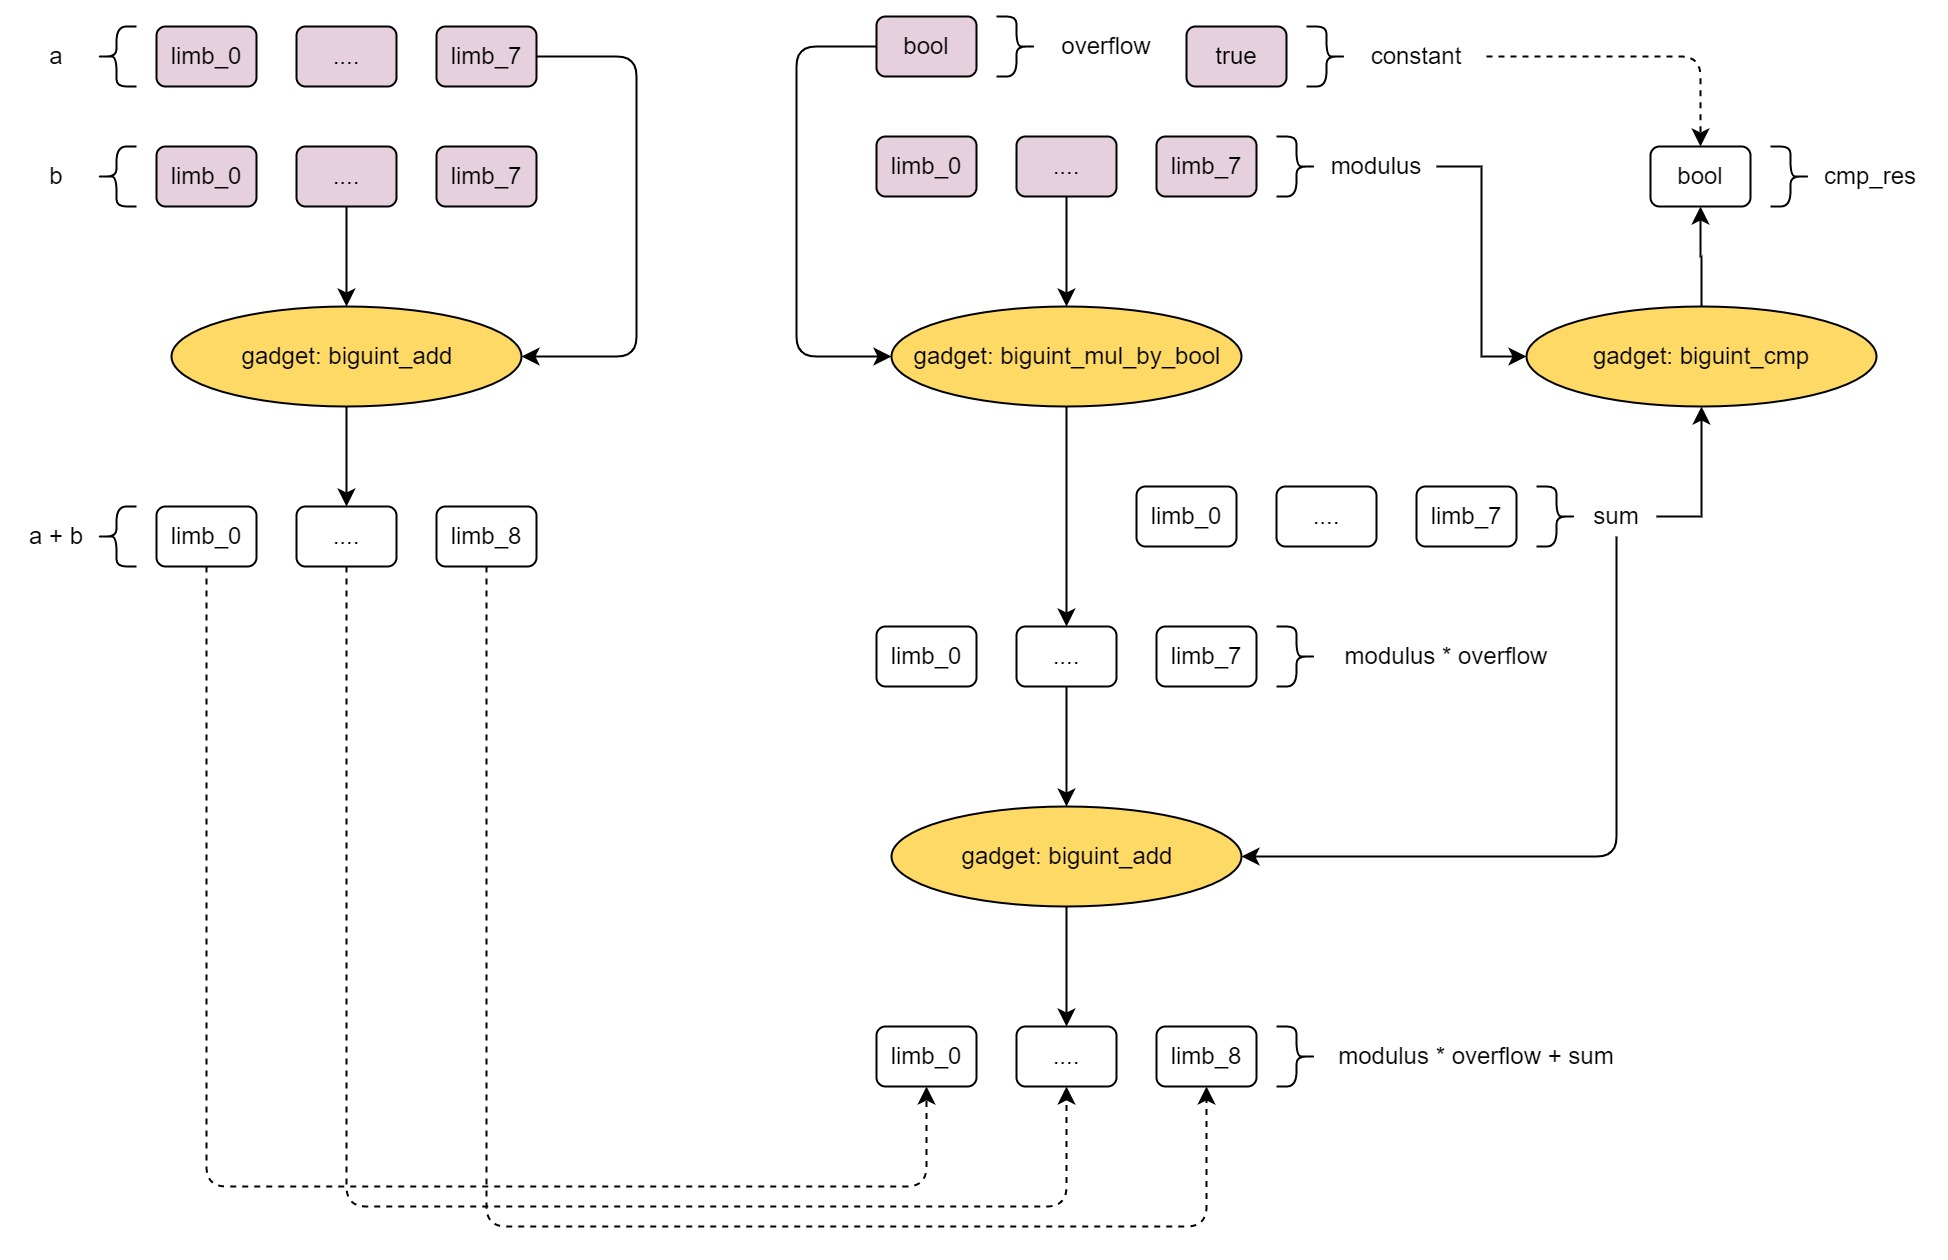
\includegraphics[width=0.8\textwidth]{nonnative-add-layout.jpg}
            \caption{nonnative-add layout}
            \label{fig:nonnative-add-layout}
        \end{figure}
    
    \item constraints-info and costs
        \begin{itemize}
            \item gadget biguint-add num: 2
            \item gadget biguint-mul-by-bool num: 1
            \item gadget biguint-cmp num: 1
            \item gate type num: 3(U32AddManyGate, ComparisonGate, ArithmeticGate)
            \item gate instance num: 23 = 3(U32AddManyGate) + 16(ComparisonGate) + 2(ArithmeticGate(1,0)) + 1(ArithmeticGate(1,-1)) + 1(ArithmeticGate(1,1))
            \item copy-constraints: 186 = 32 * 2{biguint-add} + 9{biguint-mul-by-bool} + 9 + (4 + 9) * 8{biguint-cmp} = 186
        \end{itemize}

    \item questions
        \begin{itemize}
            \item when set value to sum?
        \end{itemize}

\end{enumerate}
    \subsubsection{nonnative-sub}
\label{nonnative-sub}

\begin{enumerate}
    \item target
        check the substract relation among three nonnative target objects.
    \item constraints-logic
        \begin{itemize}
            \item check equation for gadget,  diff + b = a + modular * overflow
            \item check that "overflow is bool"
            \item check that "diff.limbs is range U32"
        \end{itemize}
    \item nonnative-sub process layout
        \begin{figure}[!ht]
            \centering
            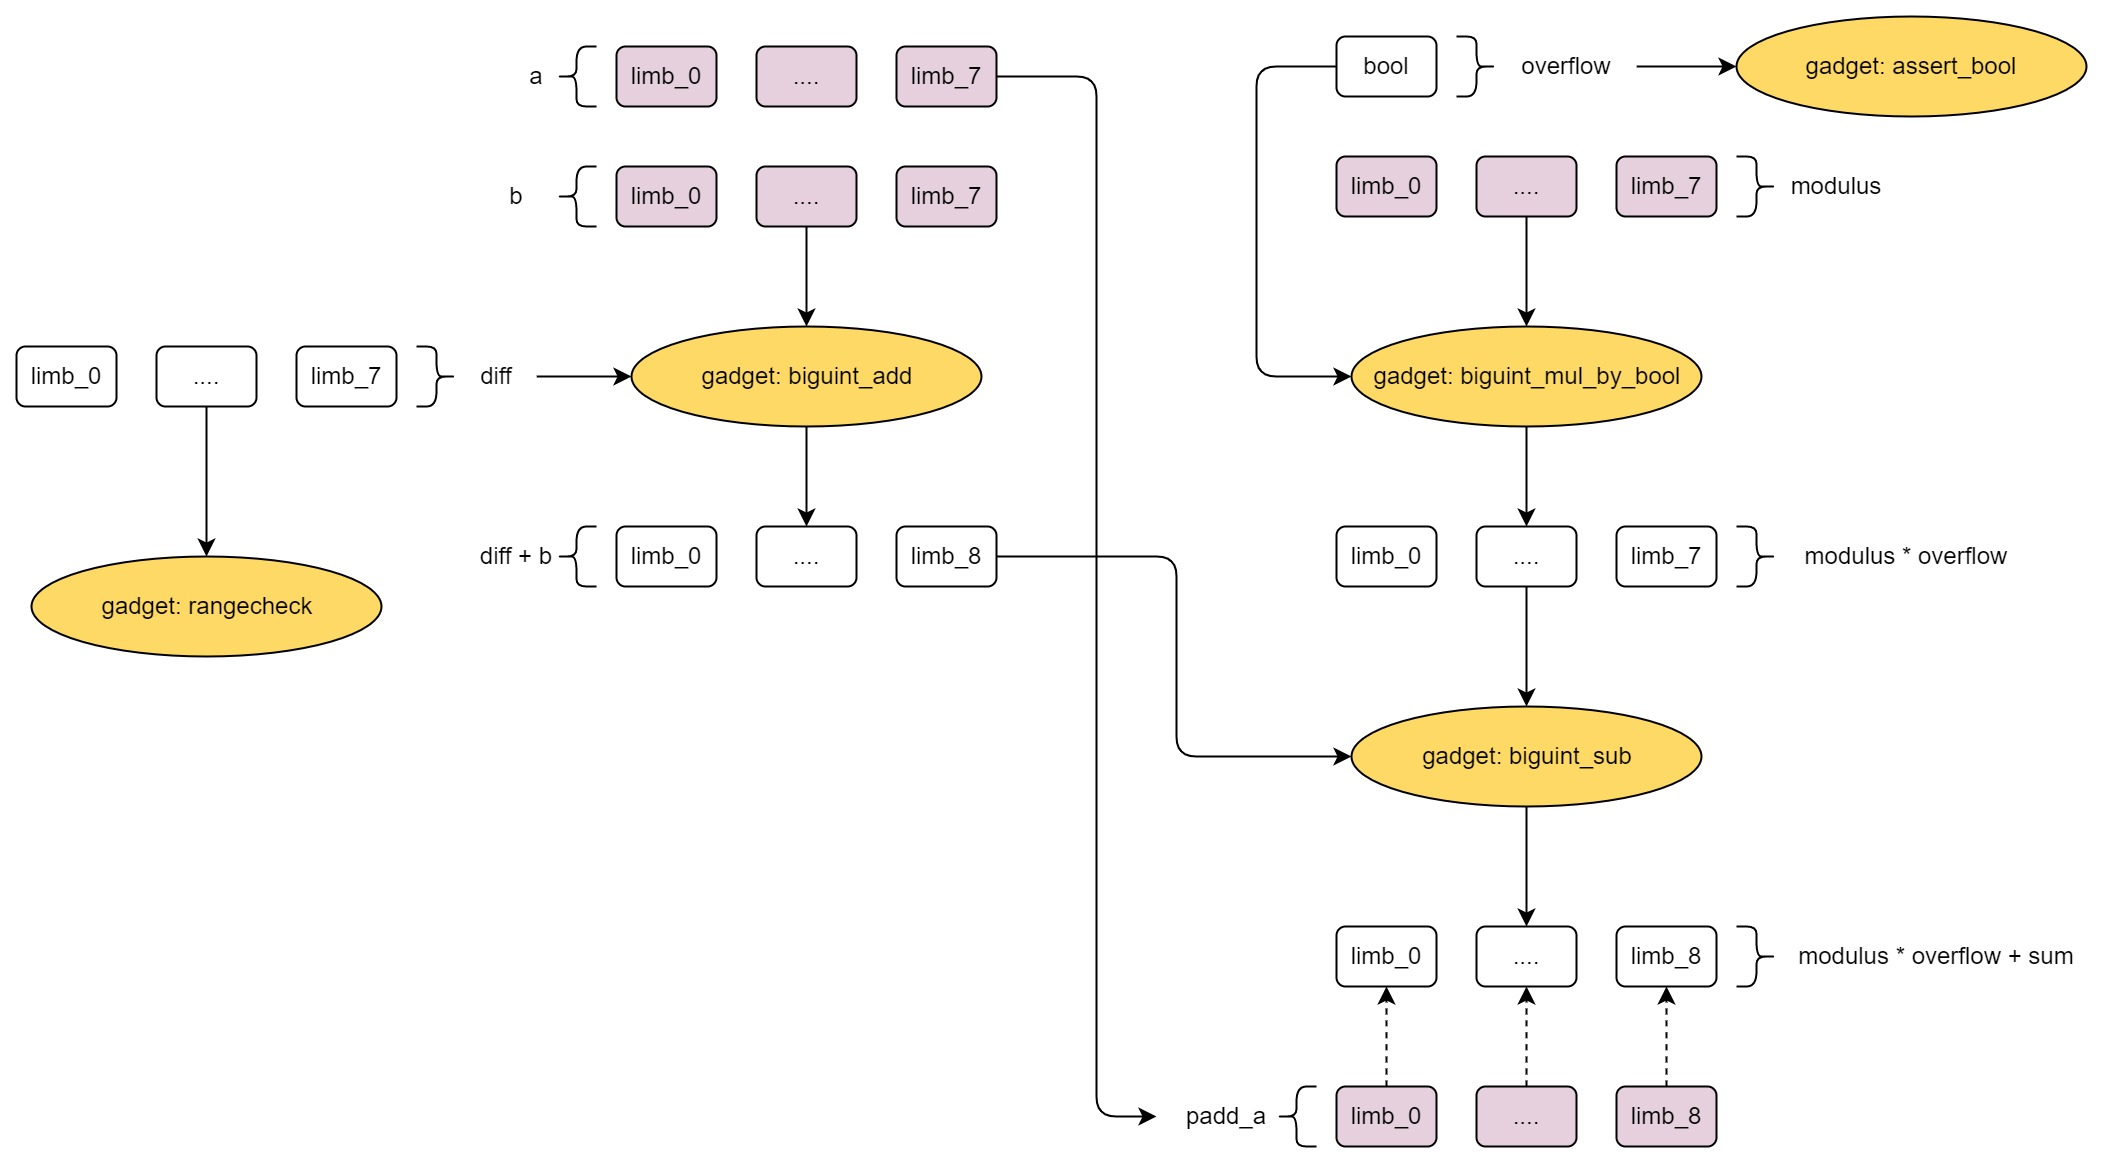
\includegraphics[width=0.8\textwidth]{nonnative-sub-layout.jpg}
            \caption{nonnative-sub layout}
            \label{fig:nonnative-sub-layout}
        \end{figure}
    
    \item constraints-info and costs
        \begin{itemize}
            \item gadget biguint-add num: 1
            \item gadget biguint-sub num: 1
            \item gadget biguint-mul-by-bool num: 1
            \item gadget u32rangecheck num: 1
            \item gadget assert-bool num: 1
            \item gate type num: 4(U32AddManyGate, U32SubtractionGate, U32RangeCheckGate, ArithmeticGate)
            \item gate instance num: 7 = 2(U32AddManyGate) + 2(U32SubtractionGate) + 1(U32RangeCheckGate) + 1(ArithmeticGate(1,0)) + 1(ArithmeticGate(1,-1))
            \item copy-constraints: 89 = 32{biguint-add num} + 27{U32SubtractionGate} + 9{biguint-mul-by-bool} + 8{u32rangecheck} + 4{assert-bool} + 9
        \end{itemize}

    \item questions
        \begin{itemize}
            \item why not constraint for overflow at nonnative-add?
            \item why not make u32rangecheck for input at nonnative-add?
        \end{itemize}

\end{enumerate}
    \subsubsection{nonnative-mul}
\label{nonnative-mul}

\begin{enumerate}
    \item target
        check the multiplicatipn relation among three nonnative target objects.
    \item constraints-logic
        \begin{itemize}
            \item check equation for gadget,  a * b = prod + modular * overflow
            \item check that "overflow.limb is U32"
            \item check that "prod.limb is U32"
        \end{itemize}
    \item nonnative-mul process layout
        \begin{figure}[!ht]
            \centering
            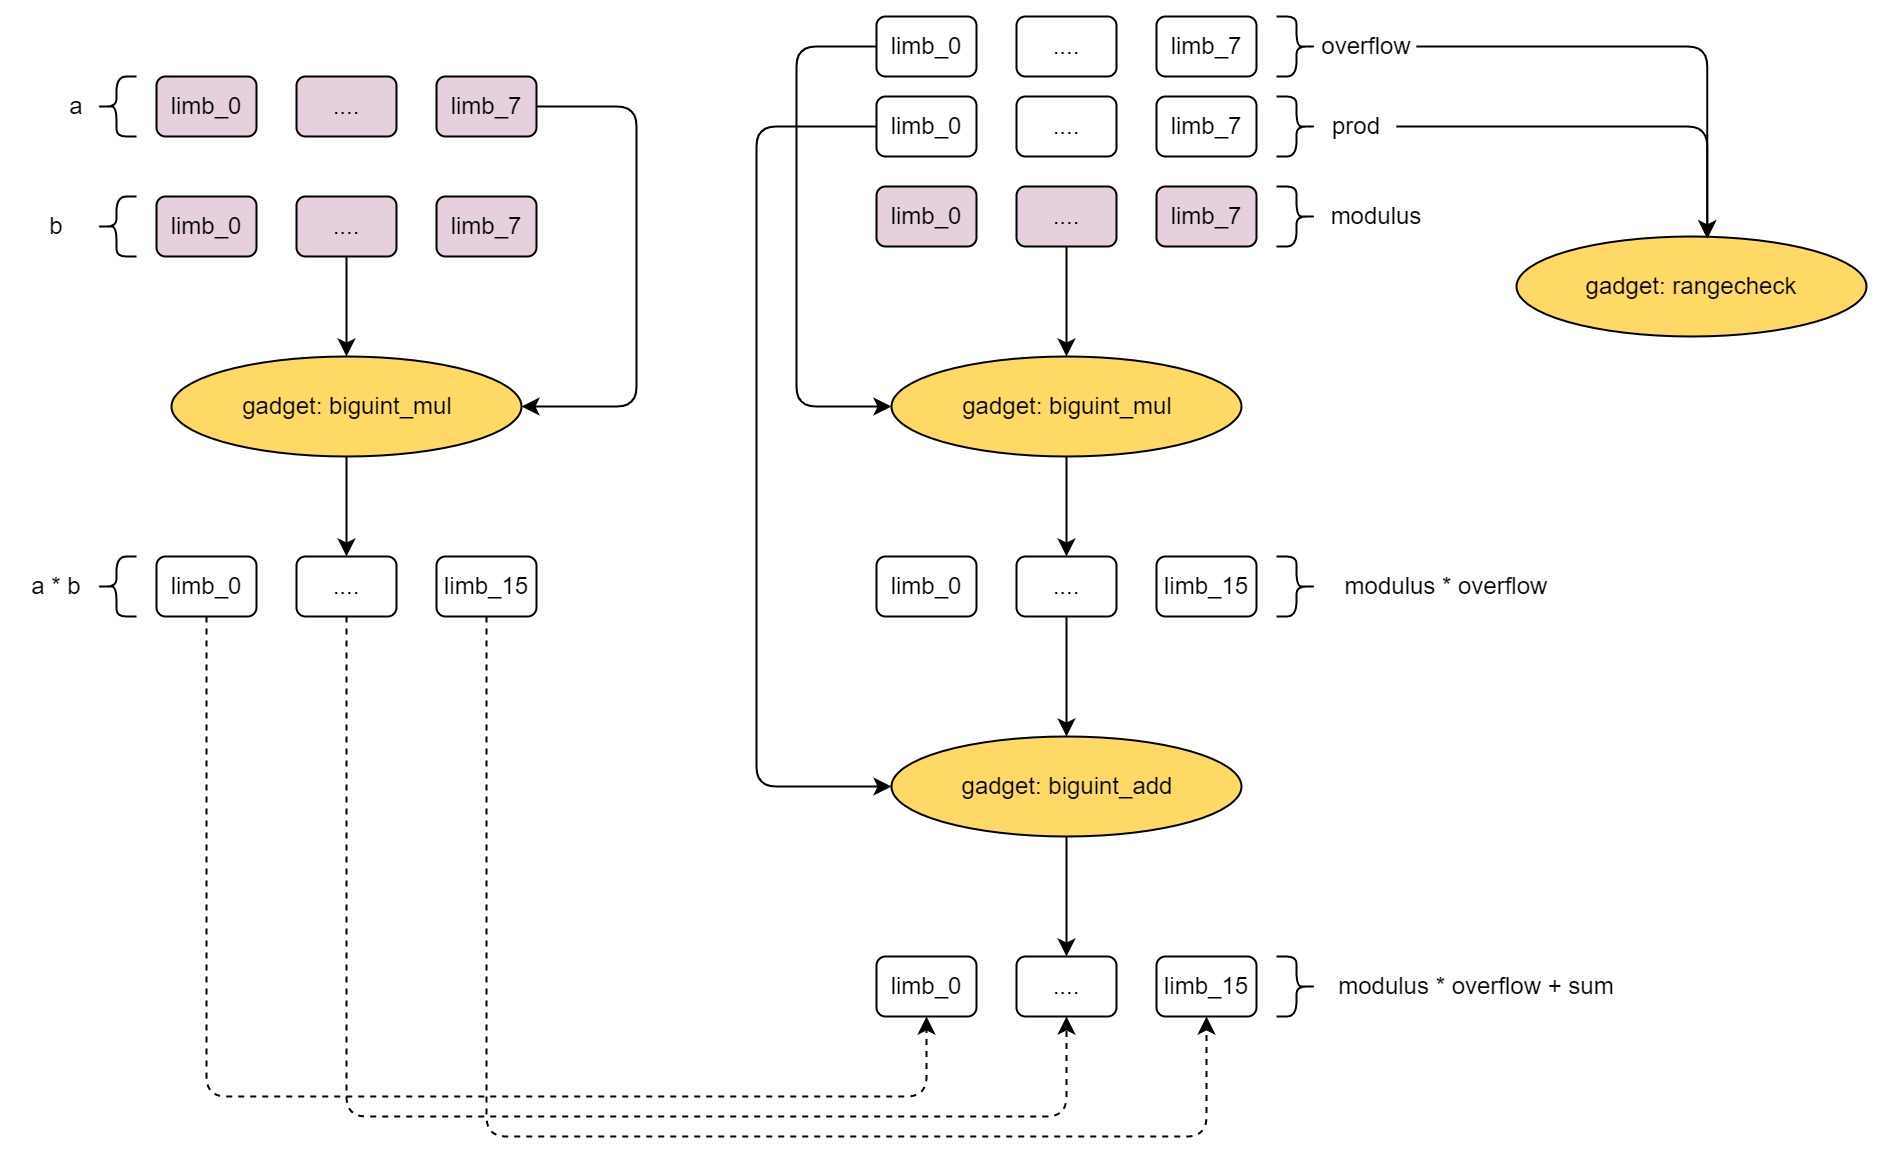
\includegraphics[width=0.8\textwidth]{nonnative-mul-layout.jpg}
            \caption{nonnative-mul layout}
            \label{fig:nonnative-mul-layout}
        \end{figure}
    
    \item constraints-info and costs
        \begin{itemize}
            \item gadget biguint-add num: 1
            \item gadget biguint-mul num: 2
            \item gadget u32rangecheck num: 2
            \item gate type num: 9 = 7(U32AddManyGate{3,5,7,9,11,13,15}) + 1(U32RangeCheckGate) + 1(U32ArithmeticGate)
            \item gate instance num: 37 = 2(u32rangecheck) + 8(biguint-mul: constant-input) + 22(biguint-mul) + 1 + 3(biguint-add)
            \item copy-constraints: 583 = 8 * 2(u32rangecheck) + 3 * 3 + (4 + 6 + 8 + 10 + 12 + 14 + 16) * 4 + (8 * 8) * 3 + 17 * 4 + 18
        \end{itemize}

\end{enumerate}
    \subsubsection{nonnative-inv}

\Par{Target}
Check the modular inverse relation among three nonnative target objects.

\Par{Constraints logic}
\begin{itemize}
    \item Check equation for gadget: \verb|a * inv_a = 1 + modular * div|.
\end{itemize}

\Par{Process layout}
See \figref{fig:nonnative-inv-layout}.
\begin{figure}[!ht]
    \centering
    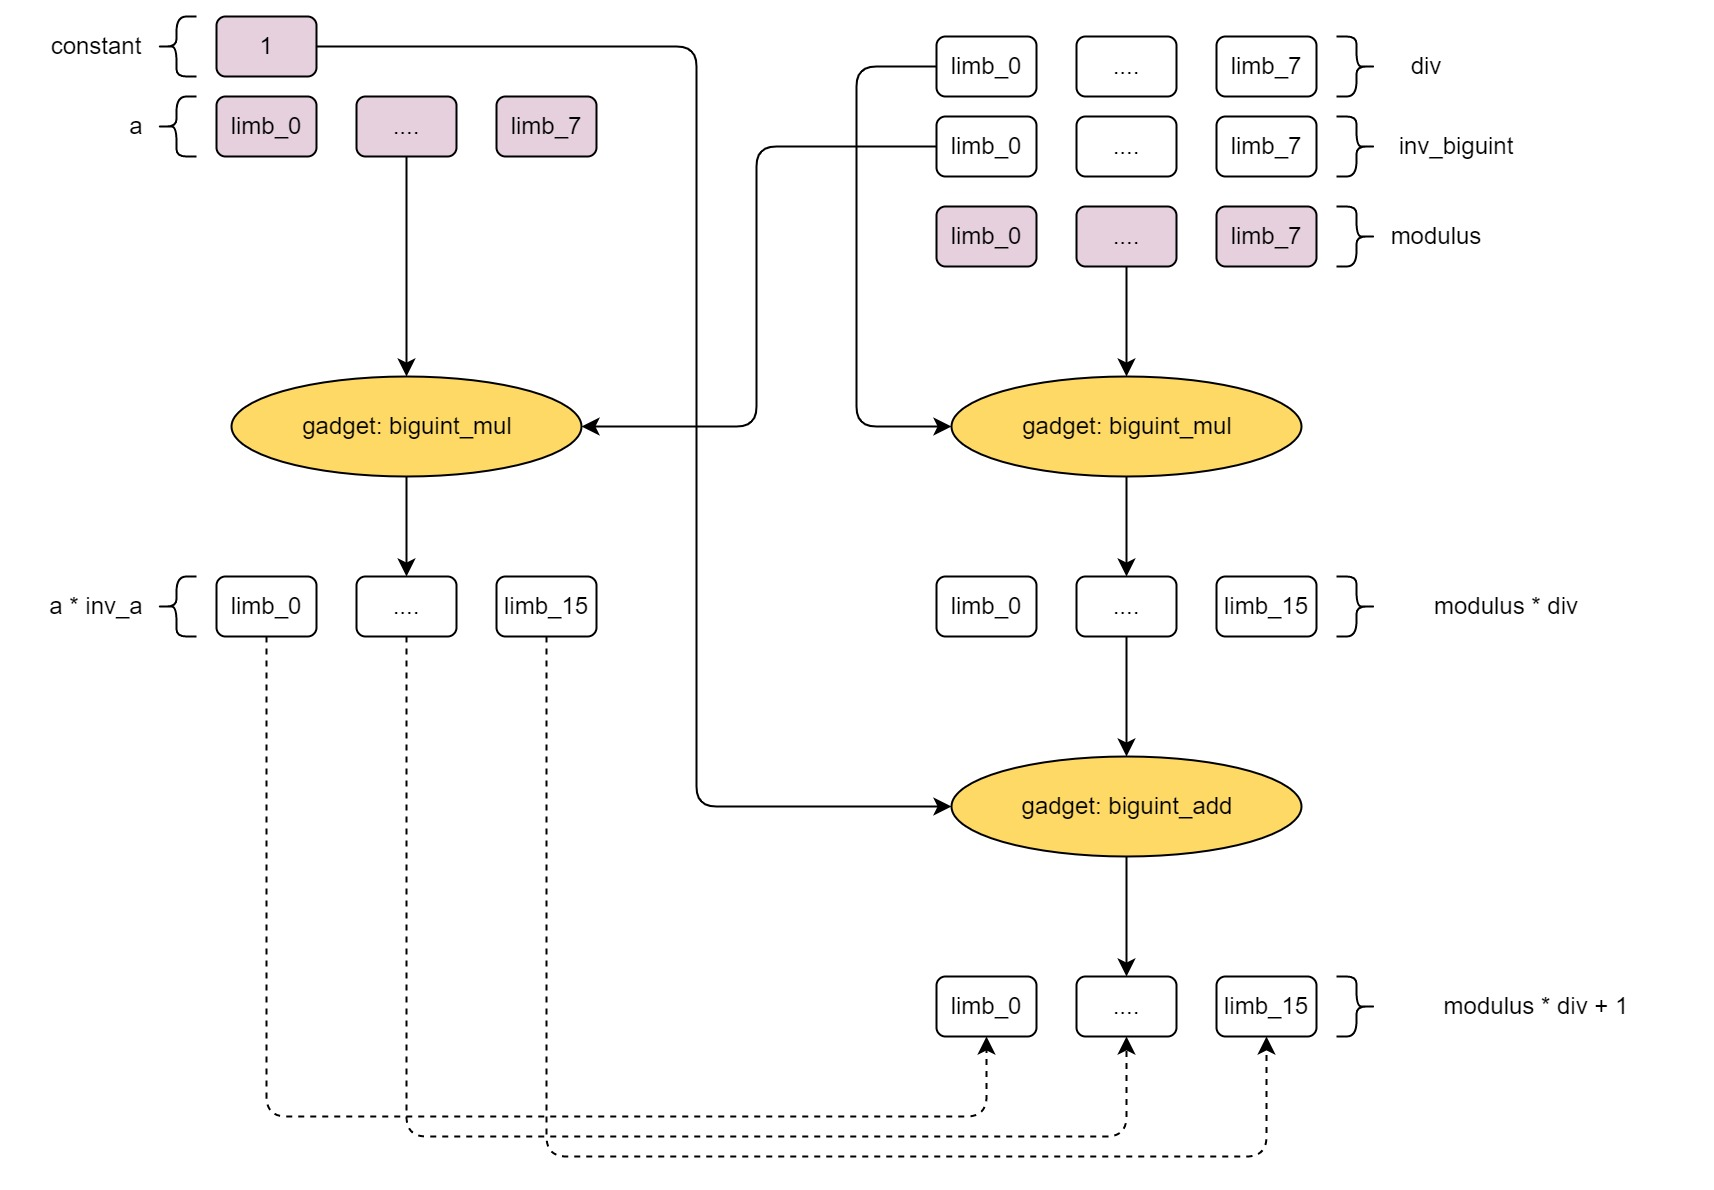
\includegraphics[width=0.8\textwidth]{nonnative-inv-layout.jpg}
    \caption{nonnative-inv layout}
    \label{fig:nonnative-inv-layout}
\end{figure}

\Par{Constraints info and costs}
\begin{itemize}
    \item gadget biguint-add num: 1
    \item gadget biguint-mul num: 2
    \item gate type num: 8 = 7(U32AddManyGate\{3,5,7,9,11,13,15\}) + 1(U32ArithmeticGate)
    \item gate instance num: 56 = (8 * 8 + 2) * 2 / 3 + 5(U32AddManyGate{3}) + 5 + 2(U32AddManyGate{15})
    \item copy-constraints: 762 = (8 * 8 + 2) * 2 * 3 + 21 * 4 + (6 + 8 + 10 + 12 + 14) * 4 + 4 * 16 + 18
\end{itemize}

    \section{curve-add}
\label{curve-add}

Take curve-secp256k1 as example, the same as other texs.

\begin{enumerate}
    \item target
        implement the addition of two different curve points. this is a incomplete addition, you can refer to The halo2 Book \cite{website:halo2-book} to learn more about it.
    \item constraints-logic
        \begin{figure}[!ht]
            \centering
            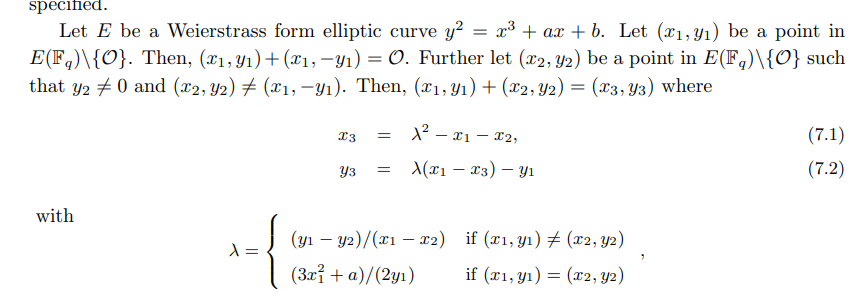
\includegraphics[width=0.8\textwidth]{curve-add.jpg}
            \caption{curve-add}
            \label{fig:curve-add}
        \end{figure}
    \item curve-add process layout
        \begin{figure}[!ht]
            \centering
            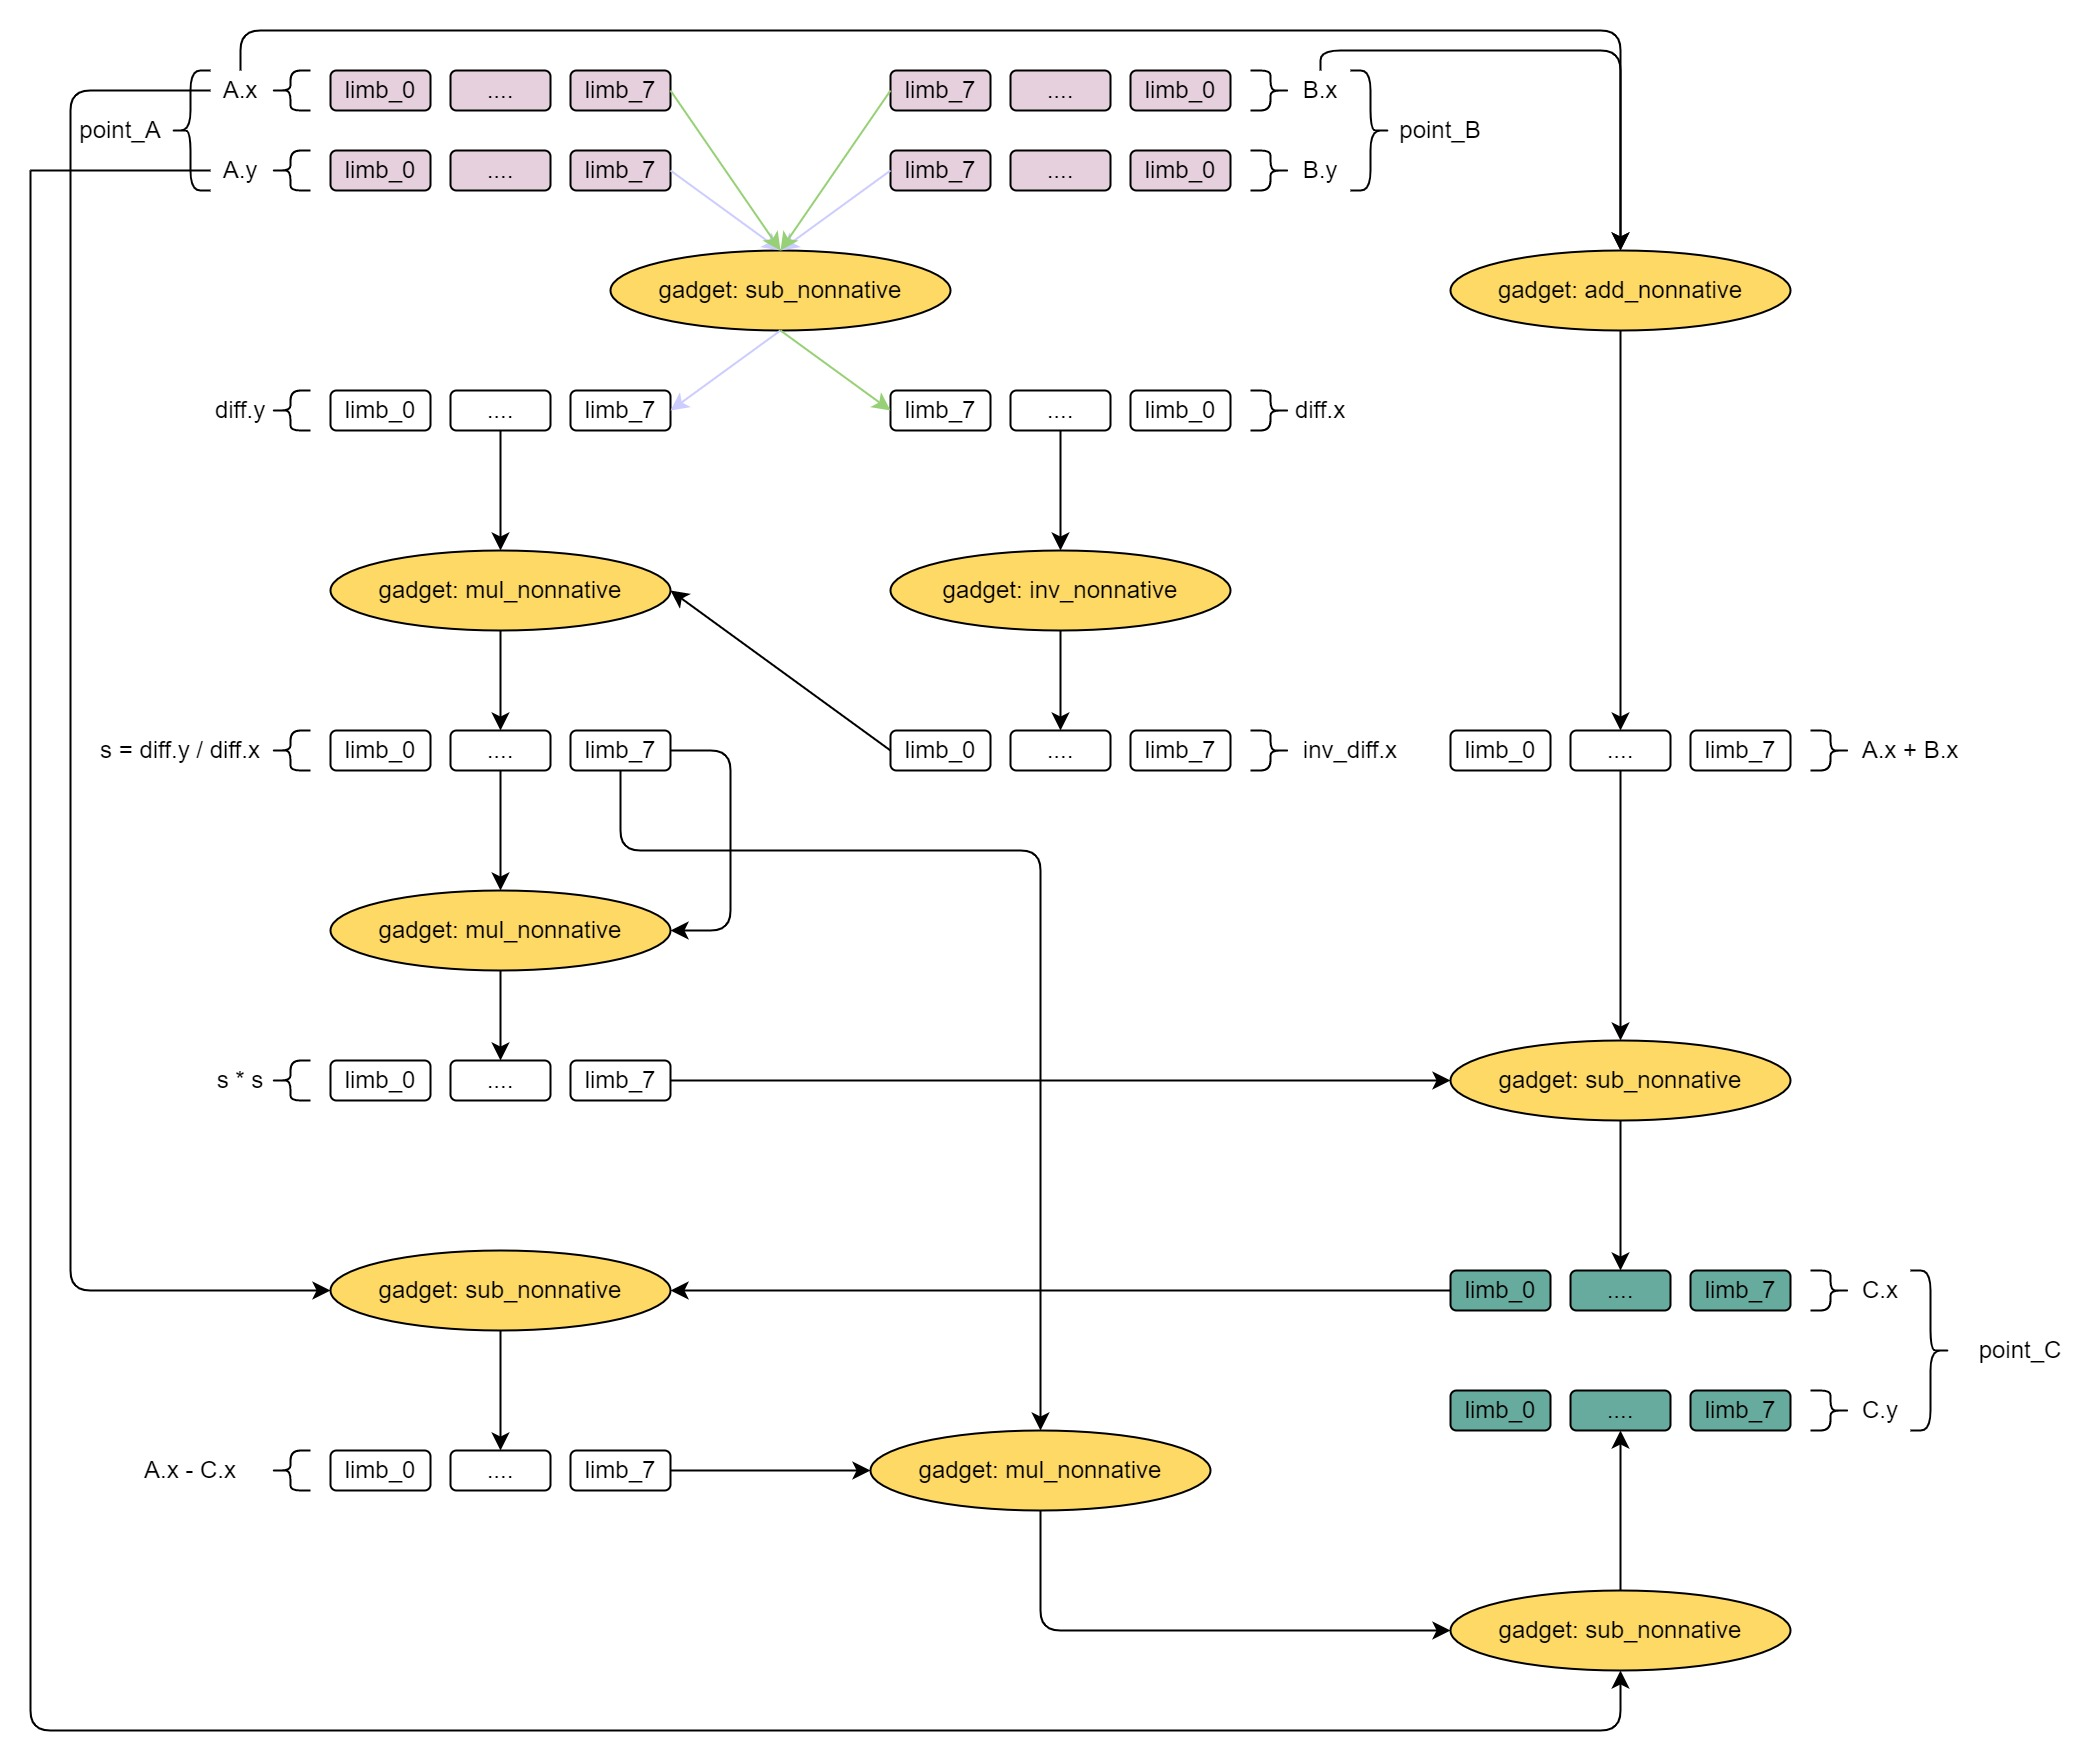
\includegraphics[width=0.8\textwidth]{curve-add-layout.jpg}
            \caption{curve-add layout}
            \label{fig:curve-add-layout}
        \end{figure}
    
    \item constraints-info and costs
        \begin{itemize}
            \item gadget-sub-nonnative num: 5
            \item gadget-add-nonnative num: 1
            \item gadget-mul-nonnative num: 3
            \item gadget-inv-nonnative num: 1
            \item gate type num: 
            \item gate instance num: 
        \end{itemize}

\end{enumerate}
    %\printbibliography[heading=bibintoc, title=\ebibname]%
\end{document}

    \subsubsection{biguint-add}

\Par{Target}
Implement the addition of two biguints.

\Par{Constraints logic}
\begin{itemize}
    \item Equation for gates;
    \item Sumcheck between output and limbs;
    \item Rangecheck for limbs.
\end{itemize}

\Par{Circuit layout}
See \figref{fig:biguint-add-circuit-layout}.
\begin{figure}[!ht]
    \centering
    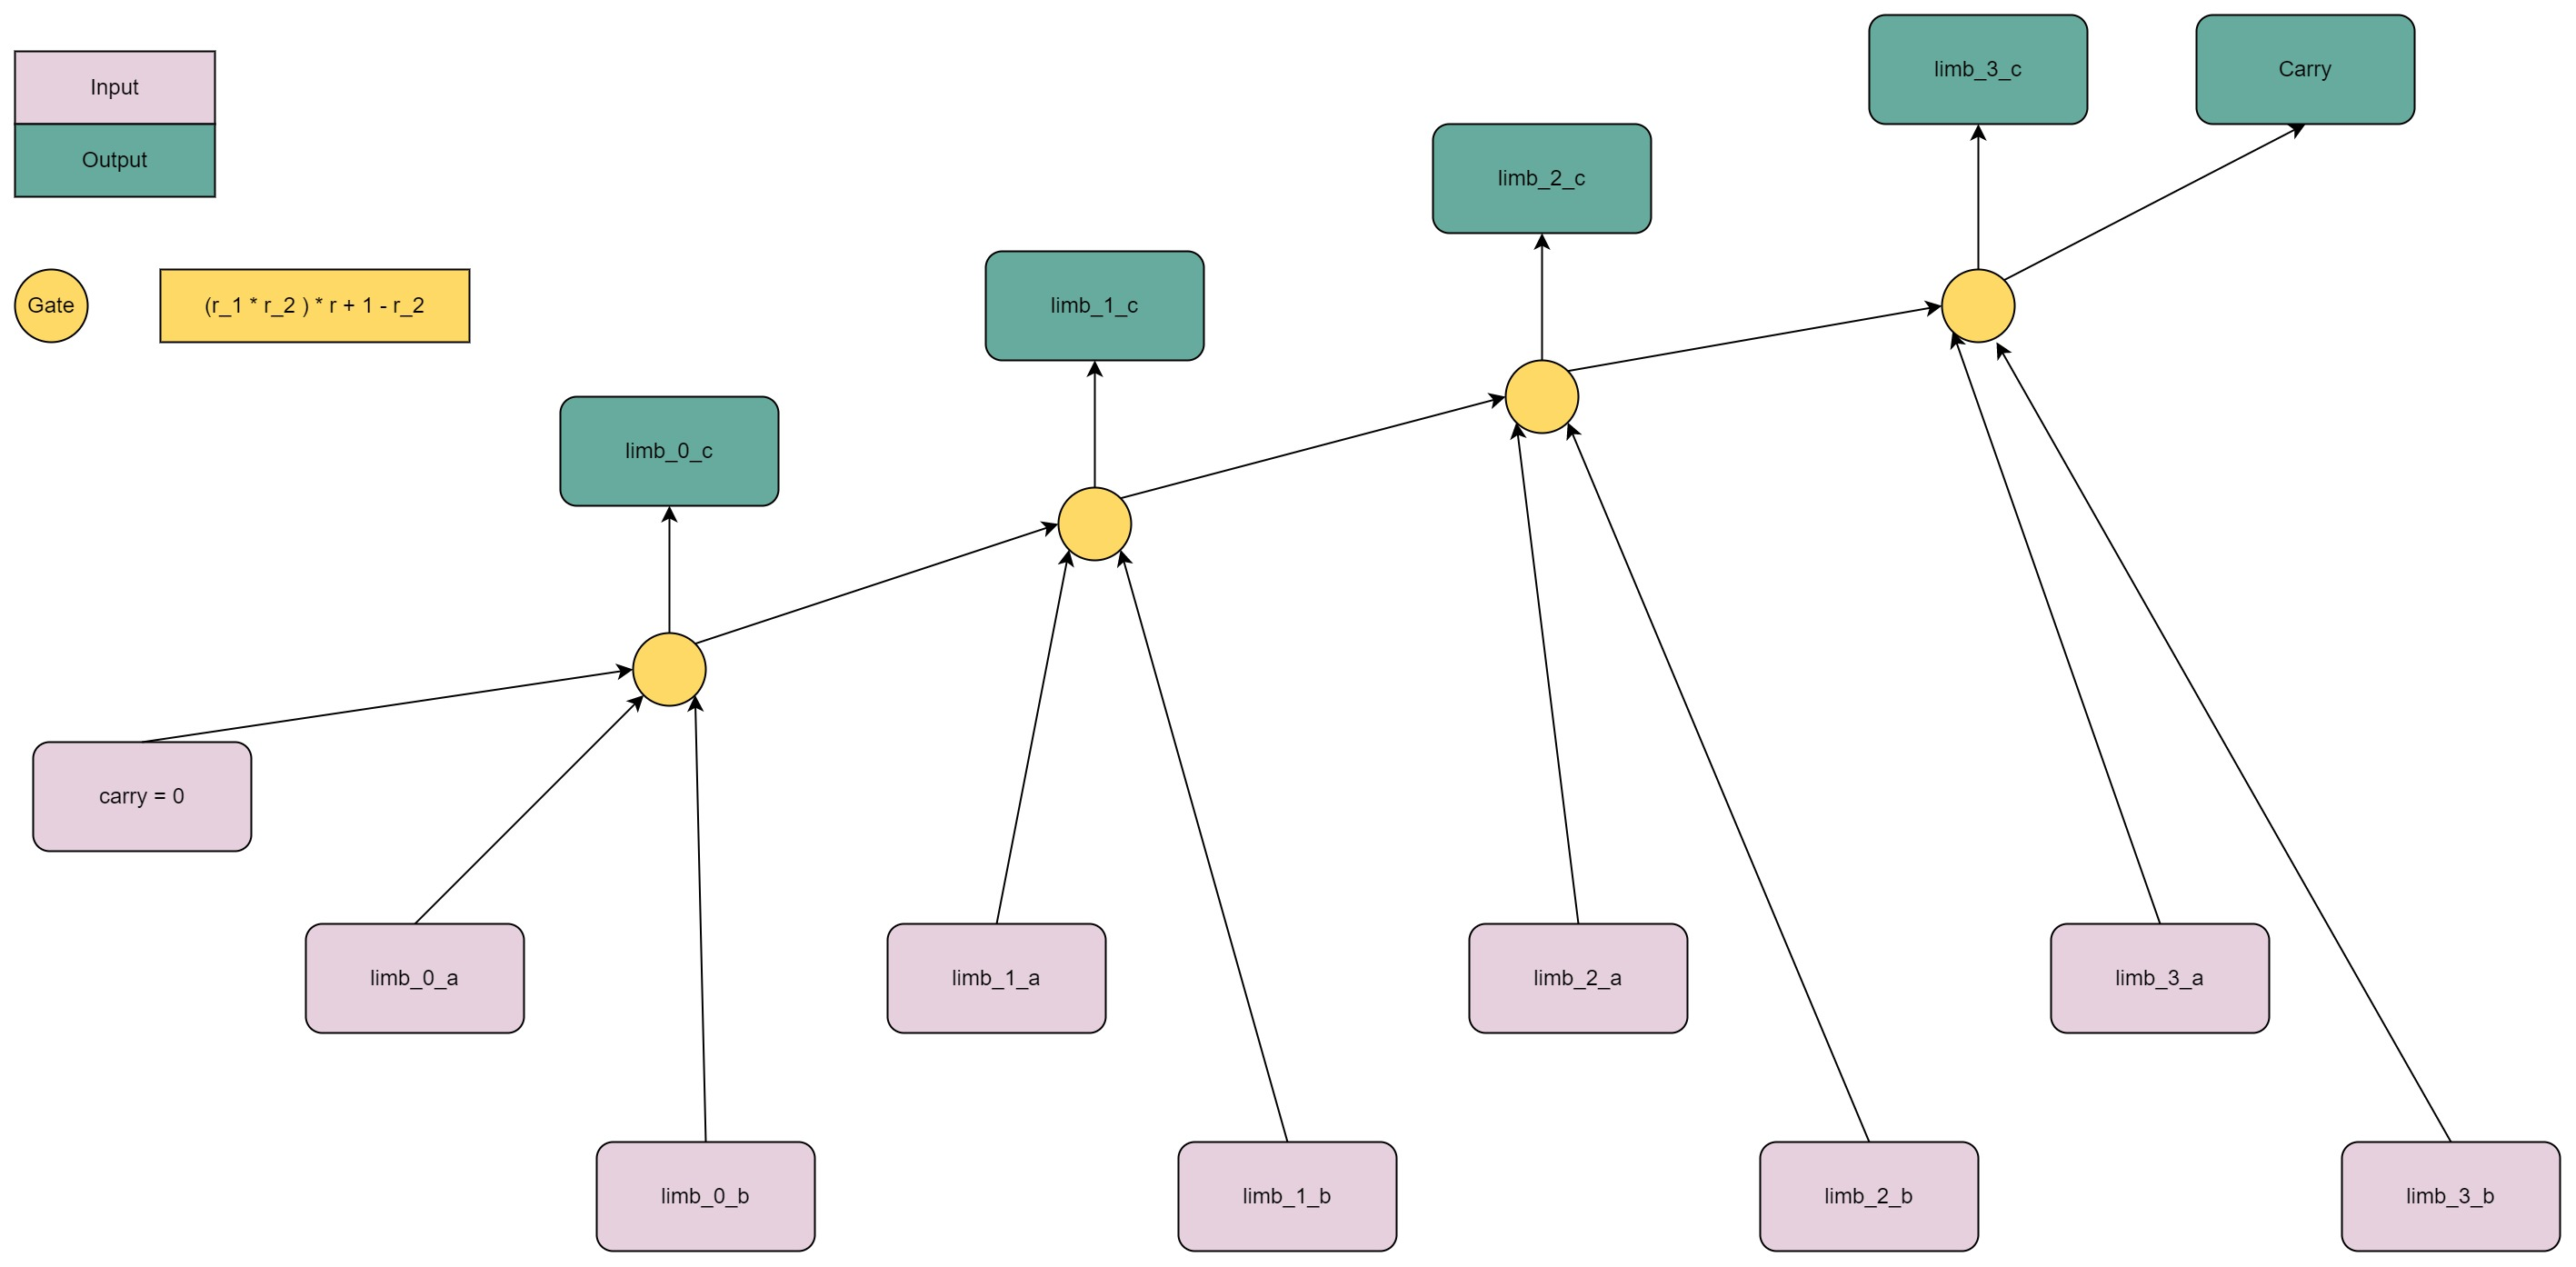
\includegraphics[width=0.8\textwidth]{biguint-add-circuit-layout.jpg}
    \caption{biguint-add circuit layout}
    \label{fig:biguint-add-circuit-layout}
\end{figure}

\Par{Trace layout}
See \figref{fig:biguint-add-trace-layout}.
\begin{figure}[!ht]
    \centering
    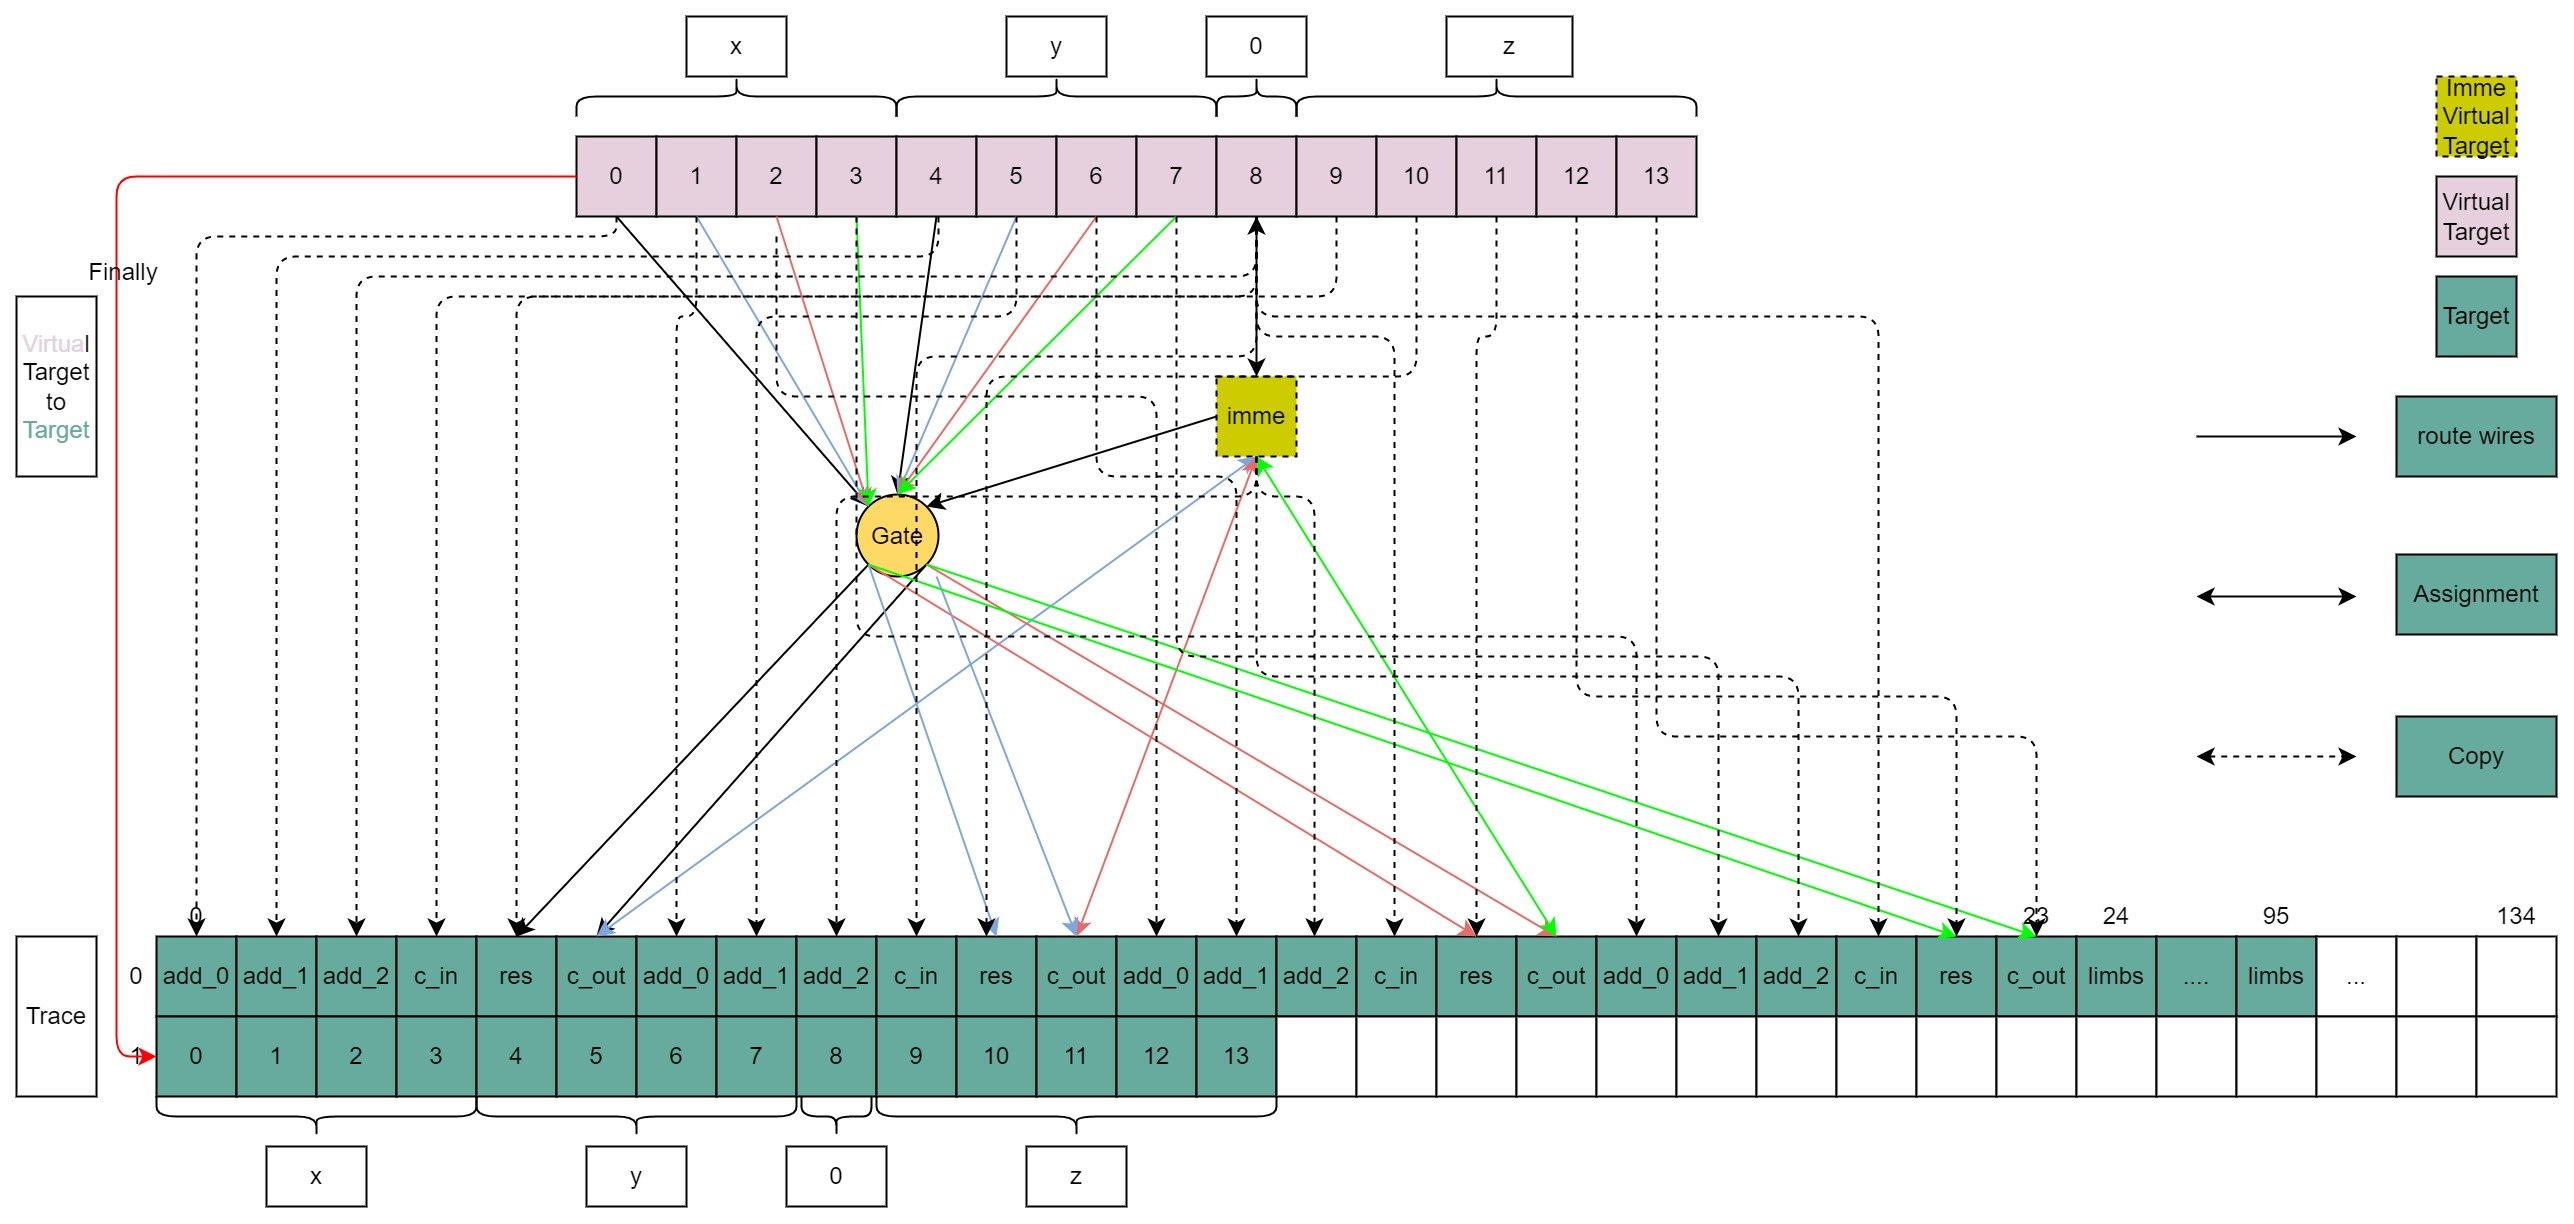
\includegraphics[width=0.8\textwidth]{biguint-add-trace-layout.jpg}
    \caption{biguint-add trace layout}
    \label{fig:biguint-add-trace-layout}
\end{figure}

\Par{Constraints info and costs}
\begin{itemize}
    \item gate type num: 1 (U32AddManyGate)
    \item gate ops num: limbs-num
    \item gate instance num: ceil(limbs-num / gate.ops)
    \item copy-constraints: limbs-num * 4
    \item max-degree: 4 (\verb|1 << limb-bits|)
\end{itemize}

\Par{Questions}
\begin{itemize}
    \item Why not make rangecheck constraint for inputs?
    \item Why not make copy constraint between cur-c-in and last-c-out?
\end{itemize}

    \subsubsection{biguint-sub}

\Par{Target}
Implement the substraction of two biguints.

\Par{Constraints logic}
\begin{itemize}
    \item Equation for gate;
    \item Sumcheck for ouptput;
    \item Rangecheck for limbs.
\end{itemize}

\Par{Circuit layout}
See \figref{fig:biguint-sub-circuit-layout}.
\begin{figure}[!ht]
    \centering
    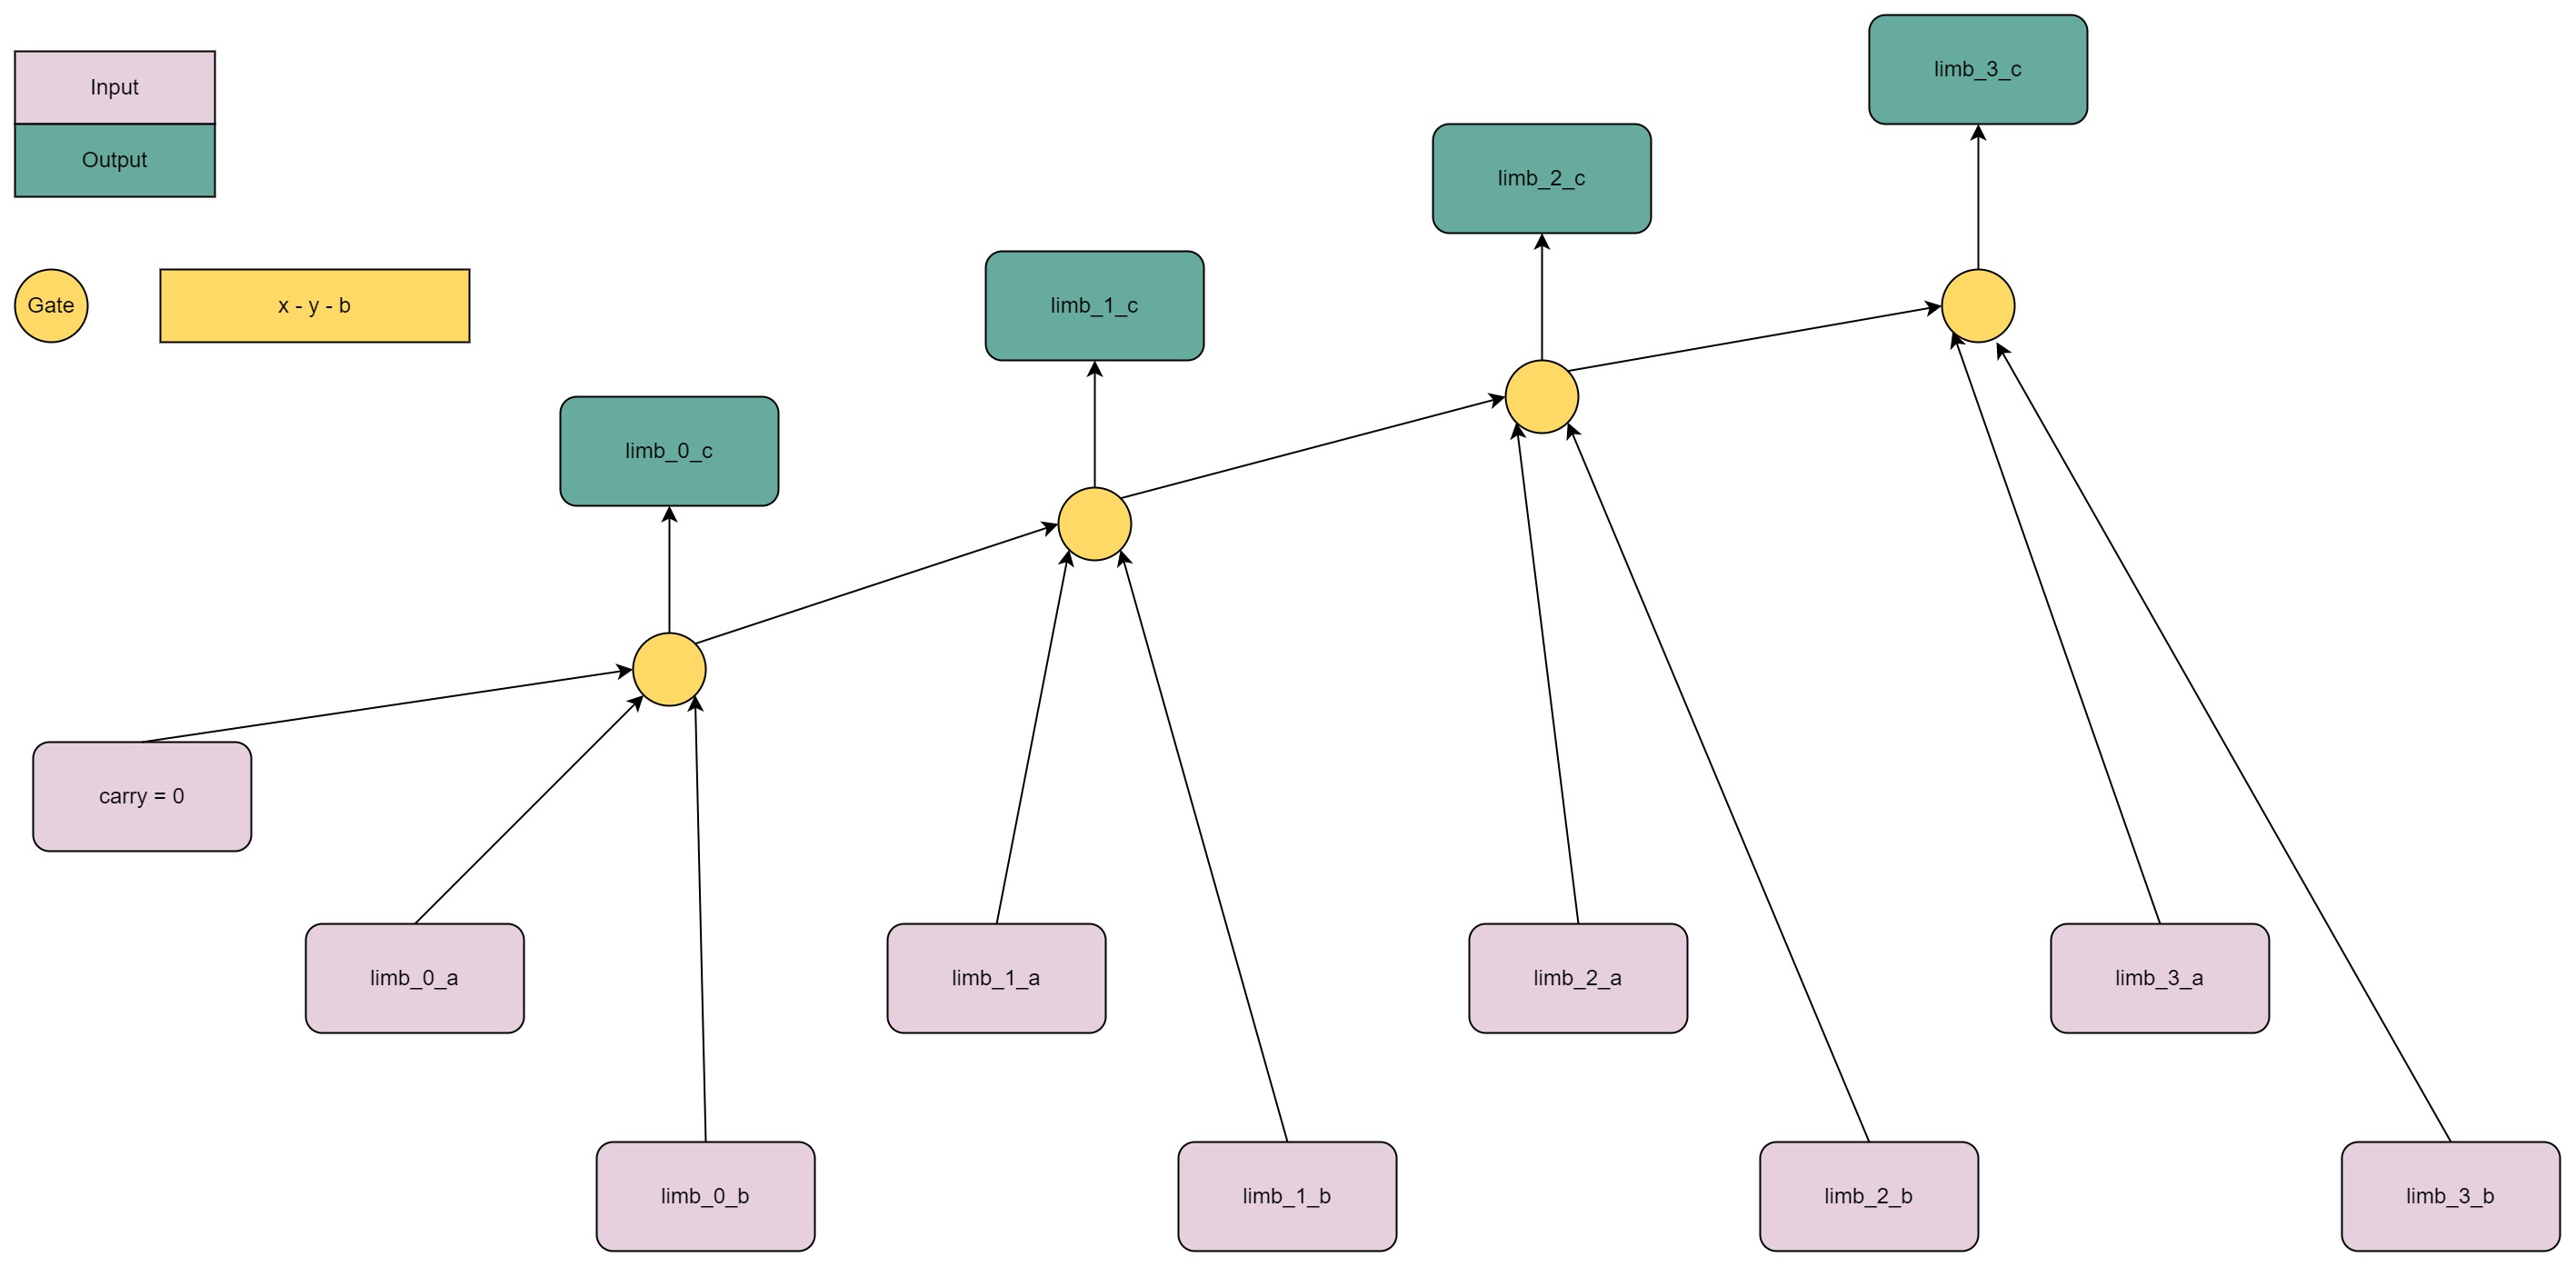
\includegraphics[width=0.8\textwidth]{biguint-sub-circuit-layout.jpg}
    \caption{biguint-sub circuit layout}
    \label{fig:biguint-sub-circuit-layout}
\end{figure}

\Par{Trace layout}
See \figref{fig:biguint-sub-trace-layout}.
\begin{figure}[!ht]
    \centering
    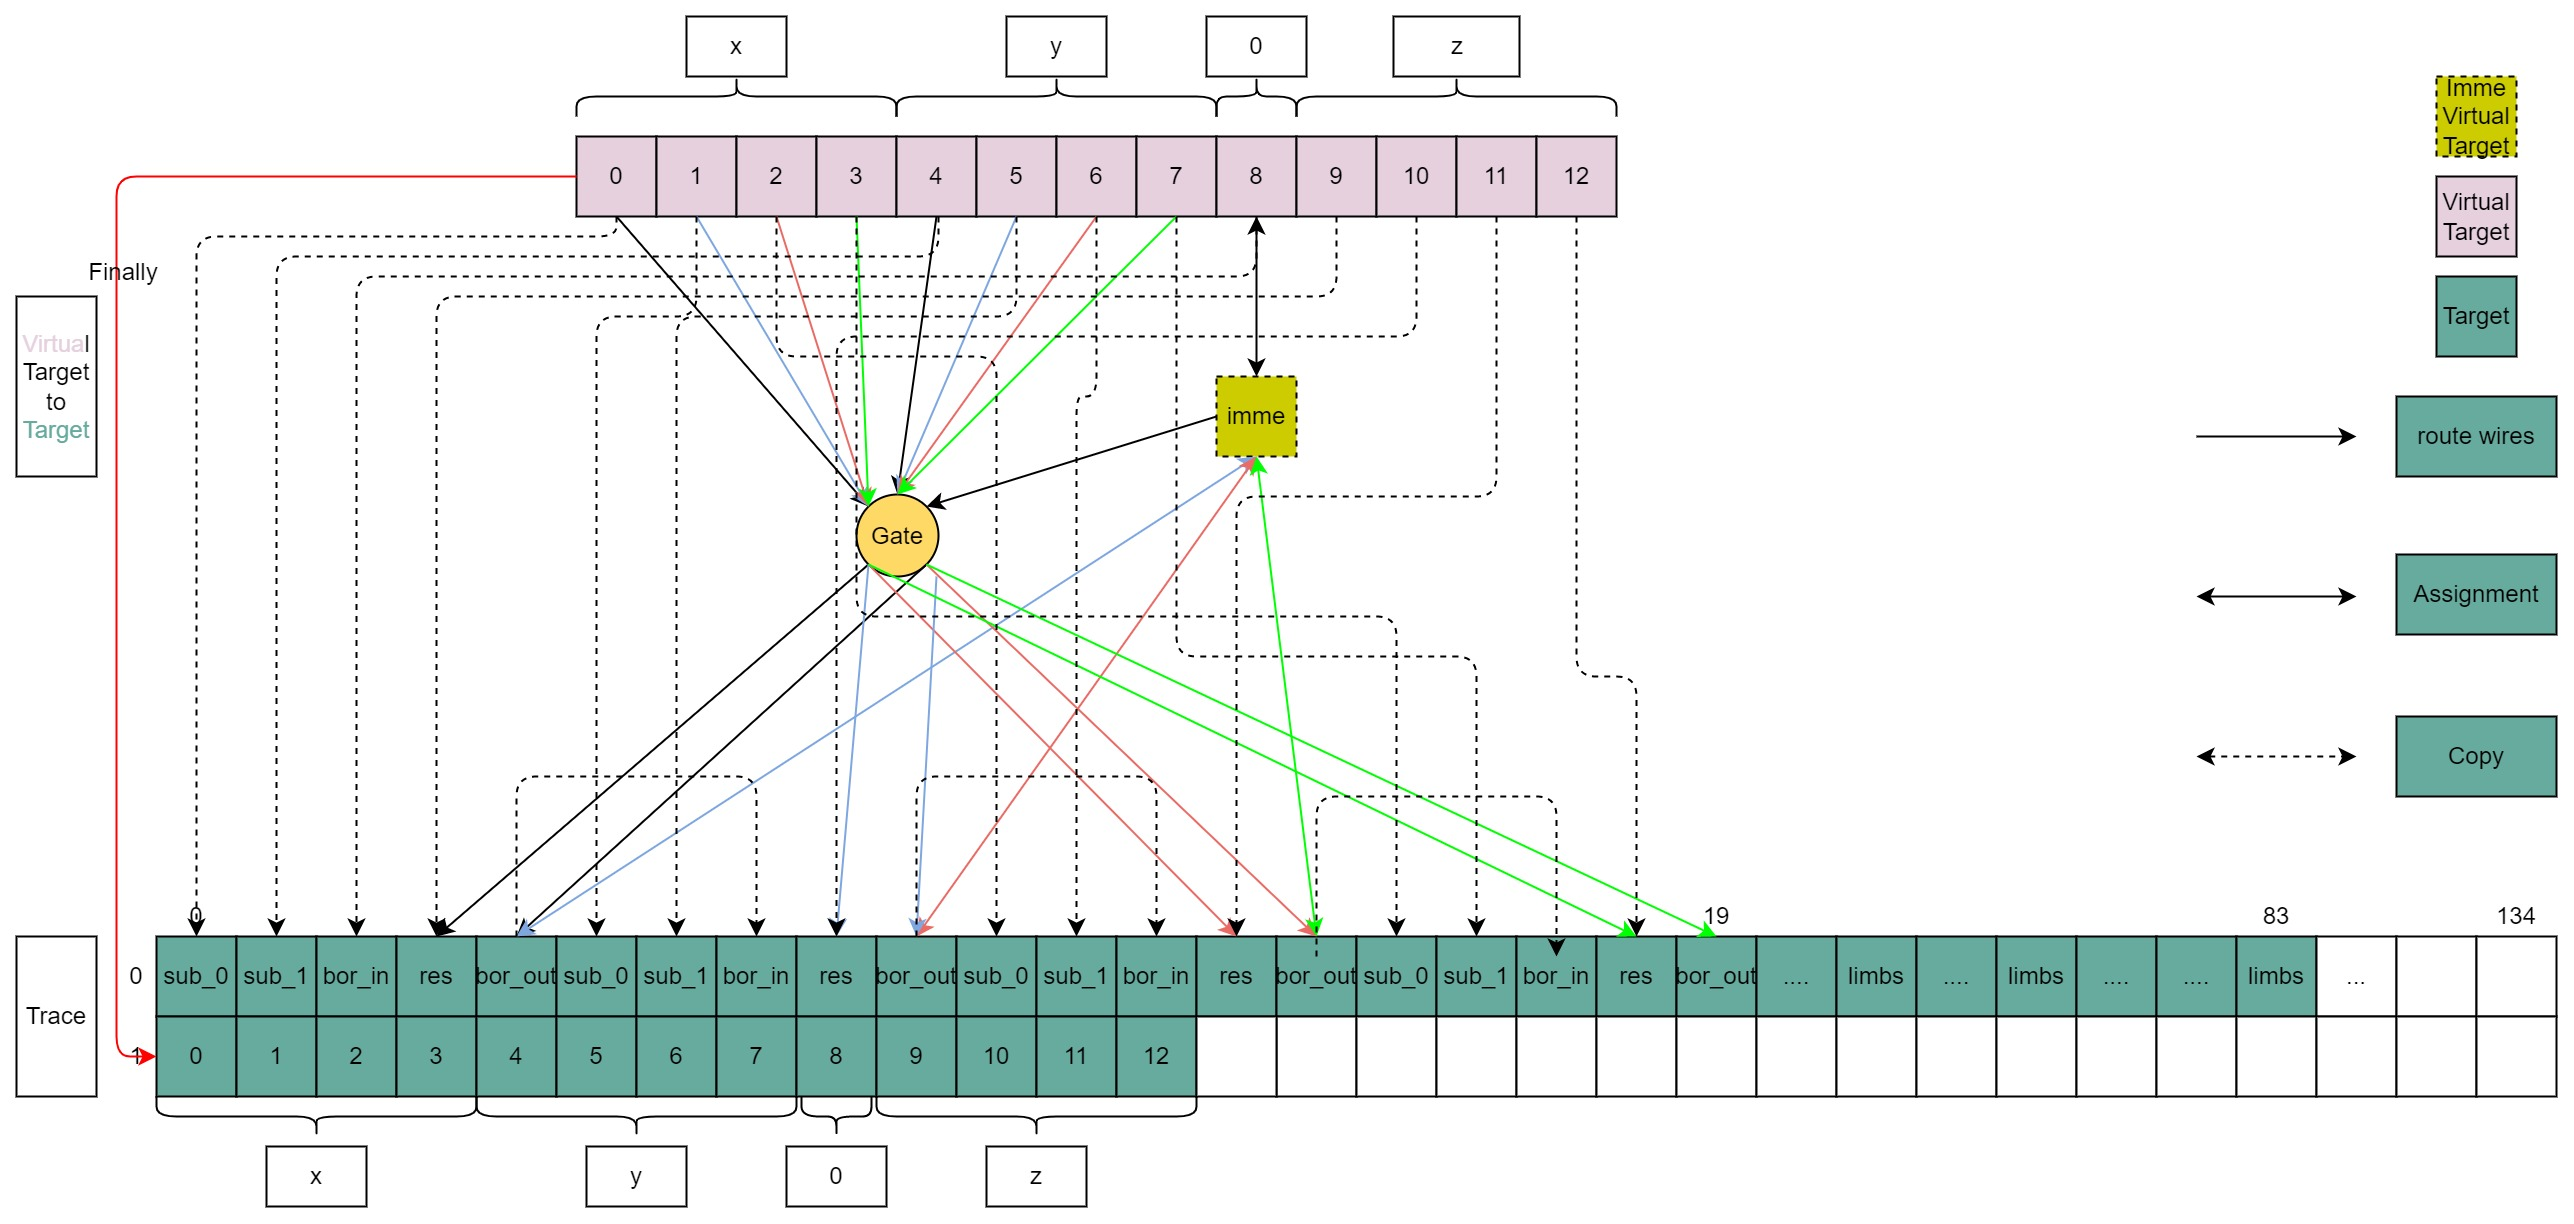
\includegraphics[width=0.8\textwidth]{biguint-sub-trace-layout.jpg}
    \caption{biguint-sub trace layout}
    \label{fig:biguint-sub-trace-layout}
\end{figure}

\Par{Constraints info and costs}
\begin{itemize}
    \item constraints-num: $6 \times (3 + 32 / 2) = 114$
    \item copy-constraints: $16$
    \item max-degree: $4$
    \item wires-num: $6 \times (5 + 16) = 126$
\end{itemize}

\Par{Questions}
\begin{itemize}
    \item Why not make rangecheck constraint for inputs?
    \item Could try to use the same constraint with add-gate.
\end{itemize}

    \subsubsection{biguint-mul}

\Par{Target}
Implement the multiplication of two biguints.

\Par{Constraints logic}
\begin{itemize}
    \item Compute mul-factors first, use U32ArithmeticGate;
    \item Add mul-factors from low bits, use U32AddManyGate.
\end{itemize}

\Par{Process layout}
See \figref{fig:biguint-mul-layout}
\begin{figure}[!ht]
    \centering
    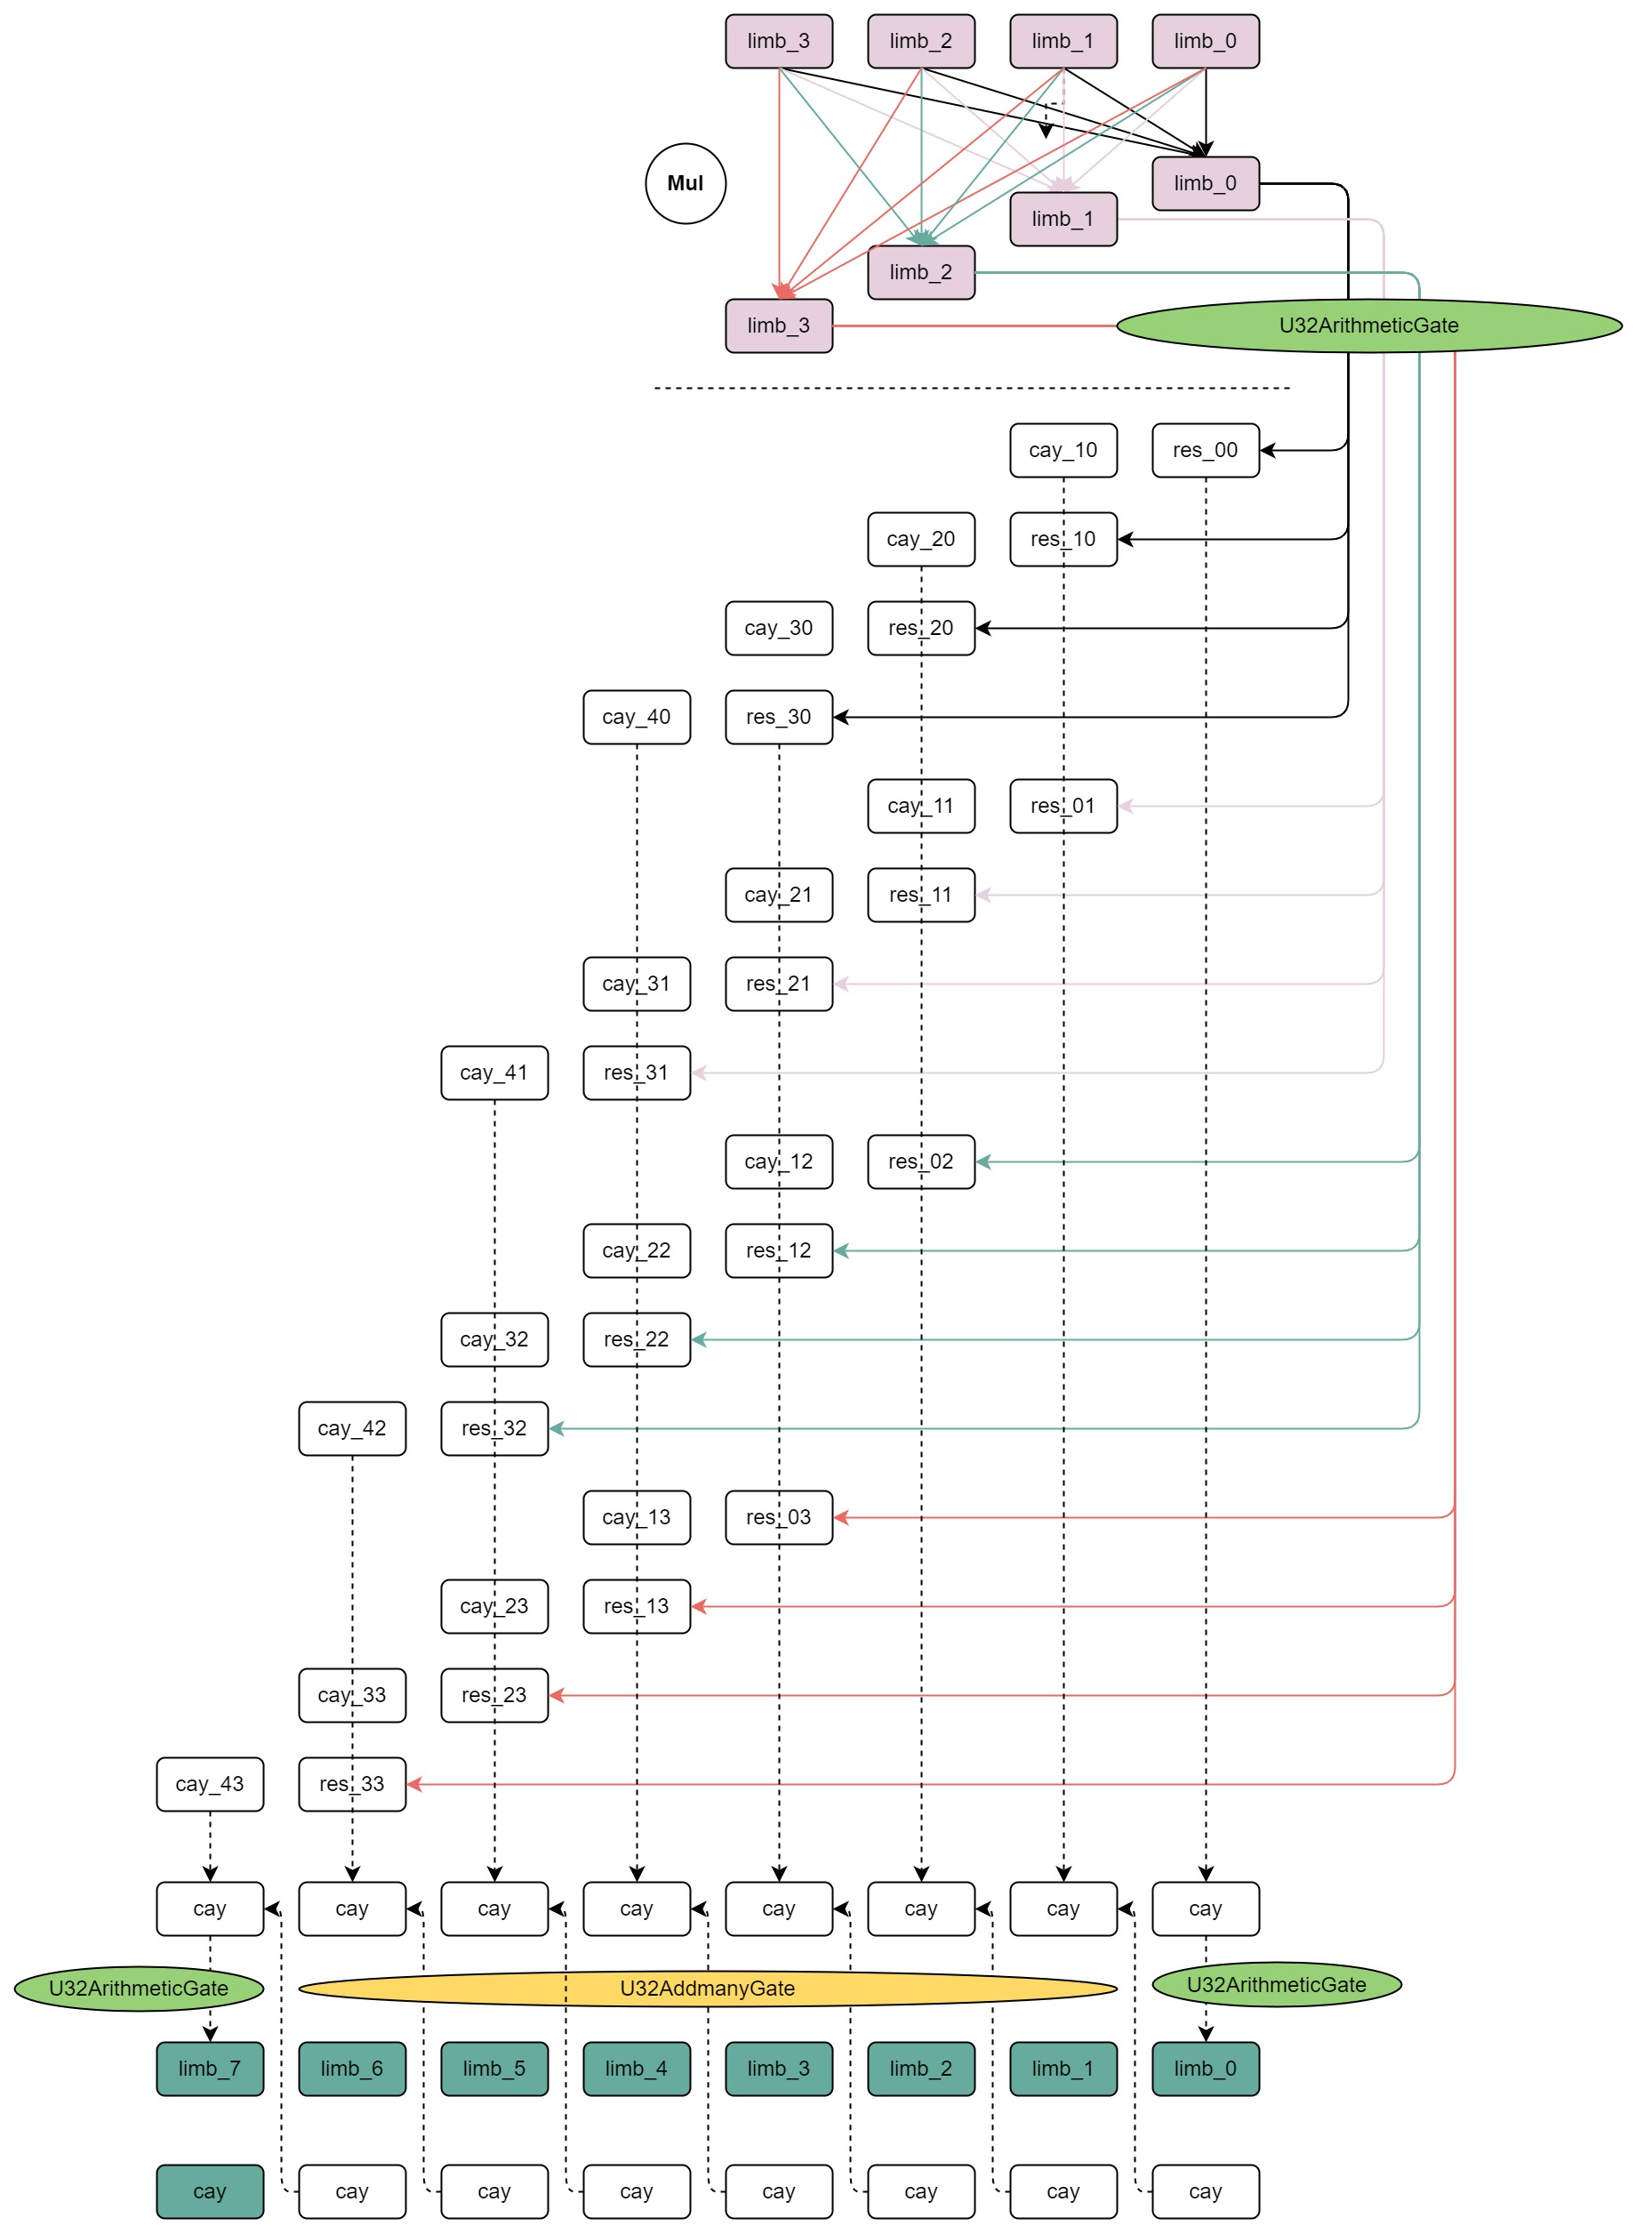
\includegraphics[width=0.8\textwidth]{biguint-mul-layout.jpg}
    \caption{biguint-mul layout}
    \label{fig:biguint-mul-layout}
\end{figure}

\Par{Constraints info and costs}
\begin{itemize}
    \item Gate type num: 4 (U32ArithmeticGate, U32AddManyGate(num-addends: 4), U32AddManyGate(num-addends: 6), U32AddManyGate(num-addends: 8))
    \item Gate instance num: 9
    \item U32ArithmeticGate num: 6
    \item U32AddManyGate num: 3
    \item copy-constraints: $18 \times 3 + (4 + 6 + 8) \times 2 + 9 = 99$
    \item max-degree: 4
\end{itemize}

    \section{biguint-div}
\label{biguint-div}

Note that div-rem has the same constraints logic with div

\begin{enumerate}
    \item target
        \begin{itemize}
            \item implement the division of two biguints
        \end{itemize}
    \item constraints-logic
        \begin{itemize}
            \item not implement div-algrithem directly
            \item use nondeterministic feature to check div-logic
            \item check div * b + rem = a
            \item check rem < b
        \end{itemize}
    \item div-process layout
        \begin{figure}[!ht]
            \centering
            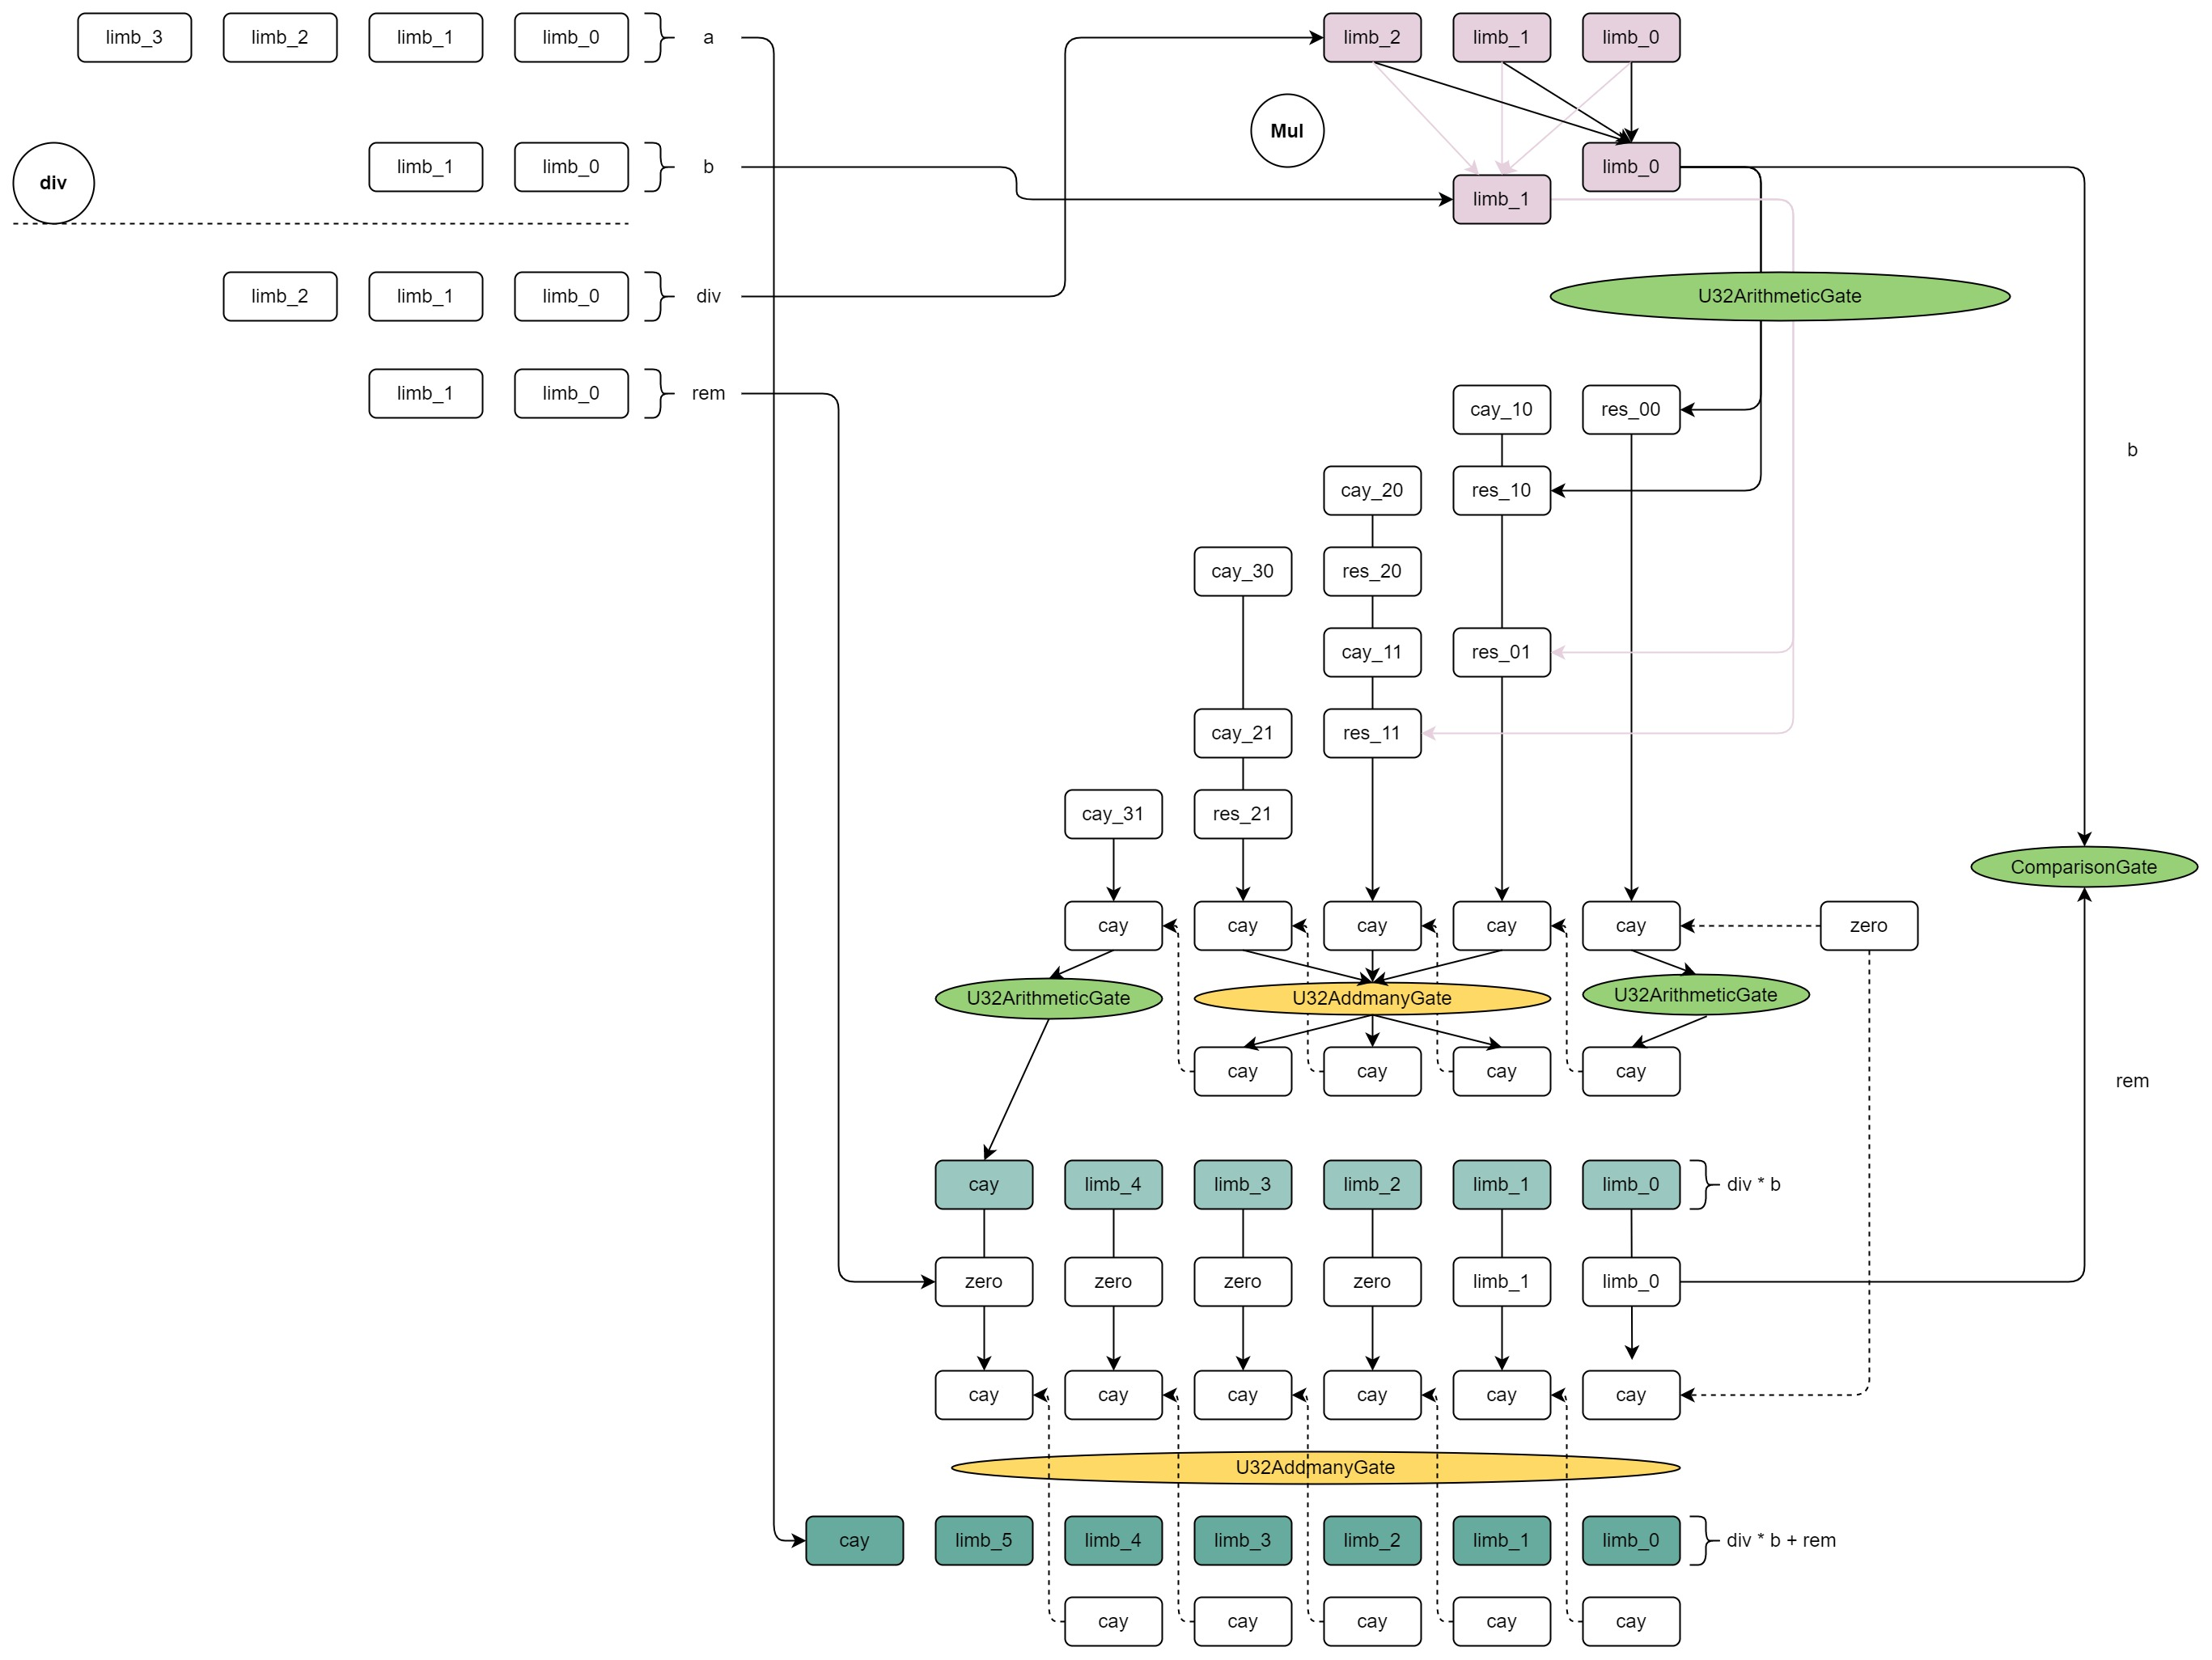
\includegraphics[width=0.8\textwidth]{biguint-div-layout.jpg}
            \caption{biguint-div layout.jpg}
            \label{fig:biguint-div-layout.jpg}
        \end{figure}
    
    \item constraints-info and costs
        \begin{itemize}
            \item Gate type num: 5(U32ArithmeticGate, U32AddManyGate(num-addends: 3), U32AddManyGate(num-addends: 4), ComparisionGate, ArithmeticGate)
            \item Gate instance num: 3 + 3 + 4 + 3 = 13 
            \item U32ArithmeticGate num: 3
            \item U32AddManyGate num: 3
            \item ComparisionGate num: 4
            \item ArithmeticGate num: 3
            \item copy-constraints: 3 * 8 + 4 + 5 + 4 + 4 * 6 + 7 + 1 + 26 + 5 = 100 
            \item max-degree: 4
        \end{itemize}

\end{enumerate}
    \subsubsection{biguint-cmp}

\Par{Target}
Implement the comparison of two biguints.

\Par{Constraints logic}
\begin{itemize}
    \item Split the input to many limbs, such that: \verb|limbs_num = bits / chunks|;
    \item Execute comparison for low bits limbs;
    \item Ensure that the result is determined by the highest limbs which are not equal.
\end{itemize}

\Par{Process layout}
See \figref{fig:biguint-cmp-layout}.
\begin{figure}[!ht]
    \centering
    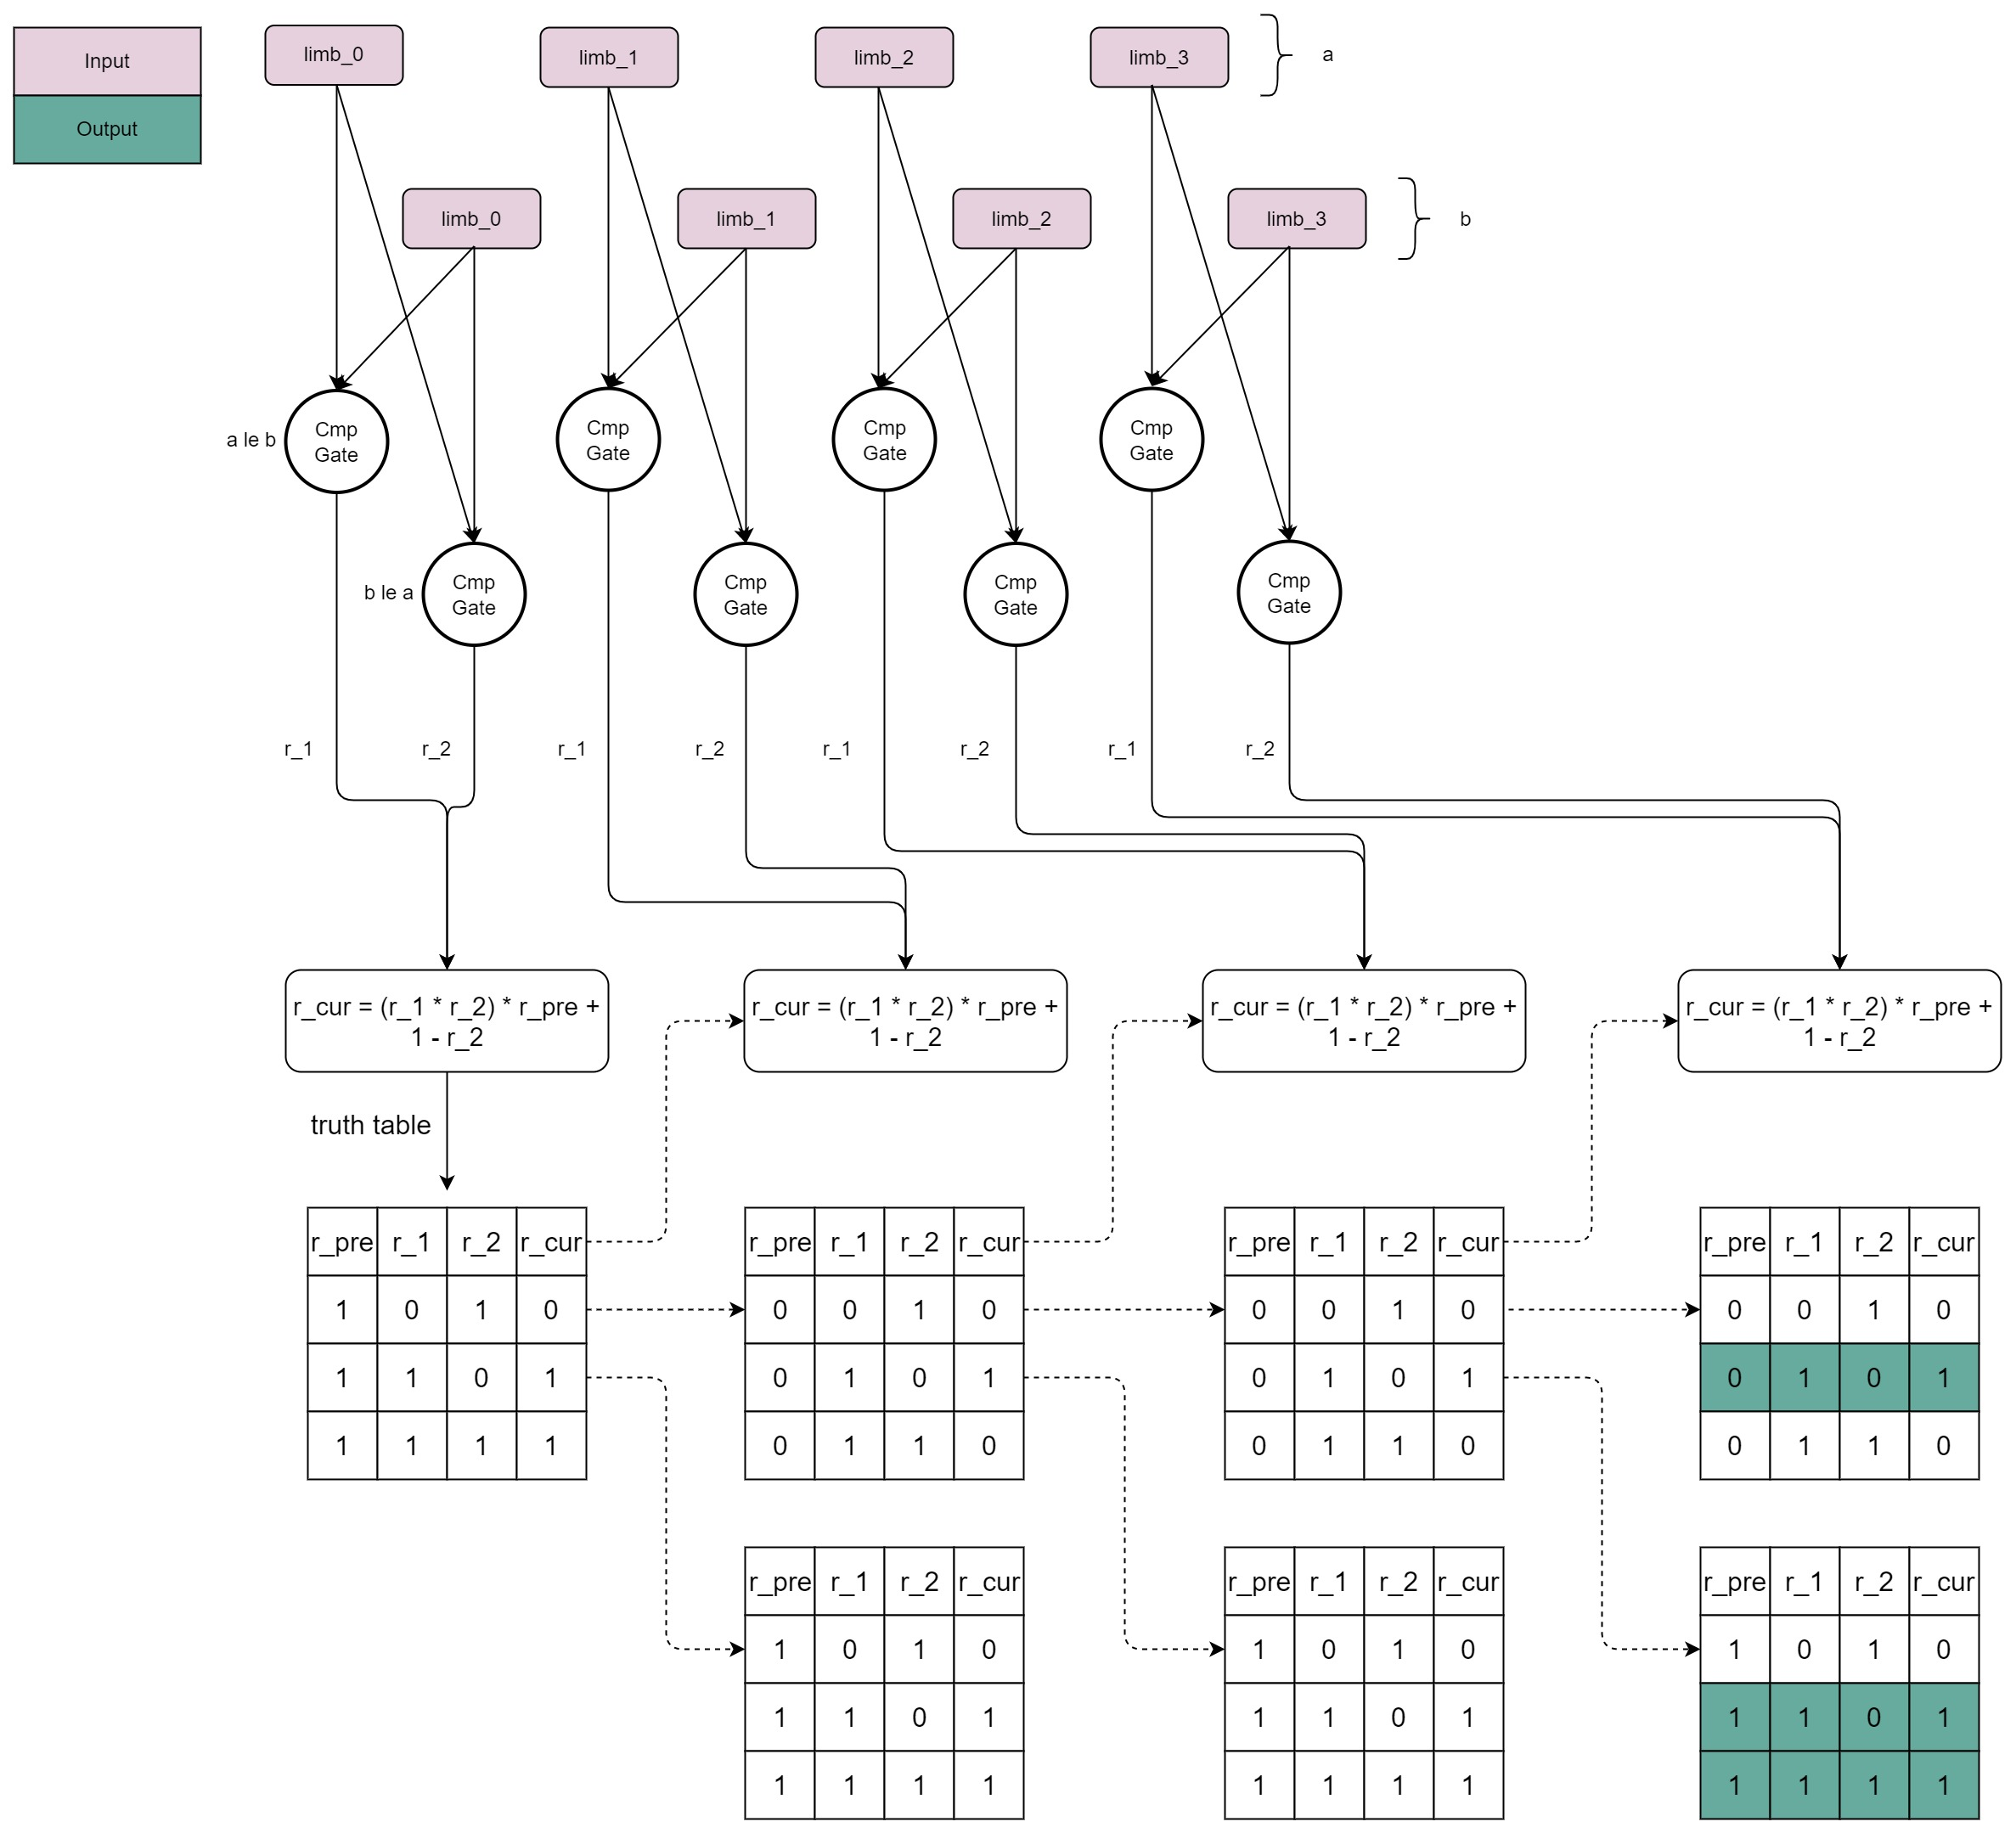
\includegraphics[width=0.8\textwidth]{biguint-cmp-layout.jpg}
    \caption{biguint-cmp layout}
    \label{fig:biguint-cmp-layout}
\end{figure}

\Par{Circuit layout}
See \figref{fig:biguint-cmp-circuit-layout}.
\begin{figure}[!ht]
    \centering
    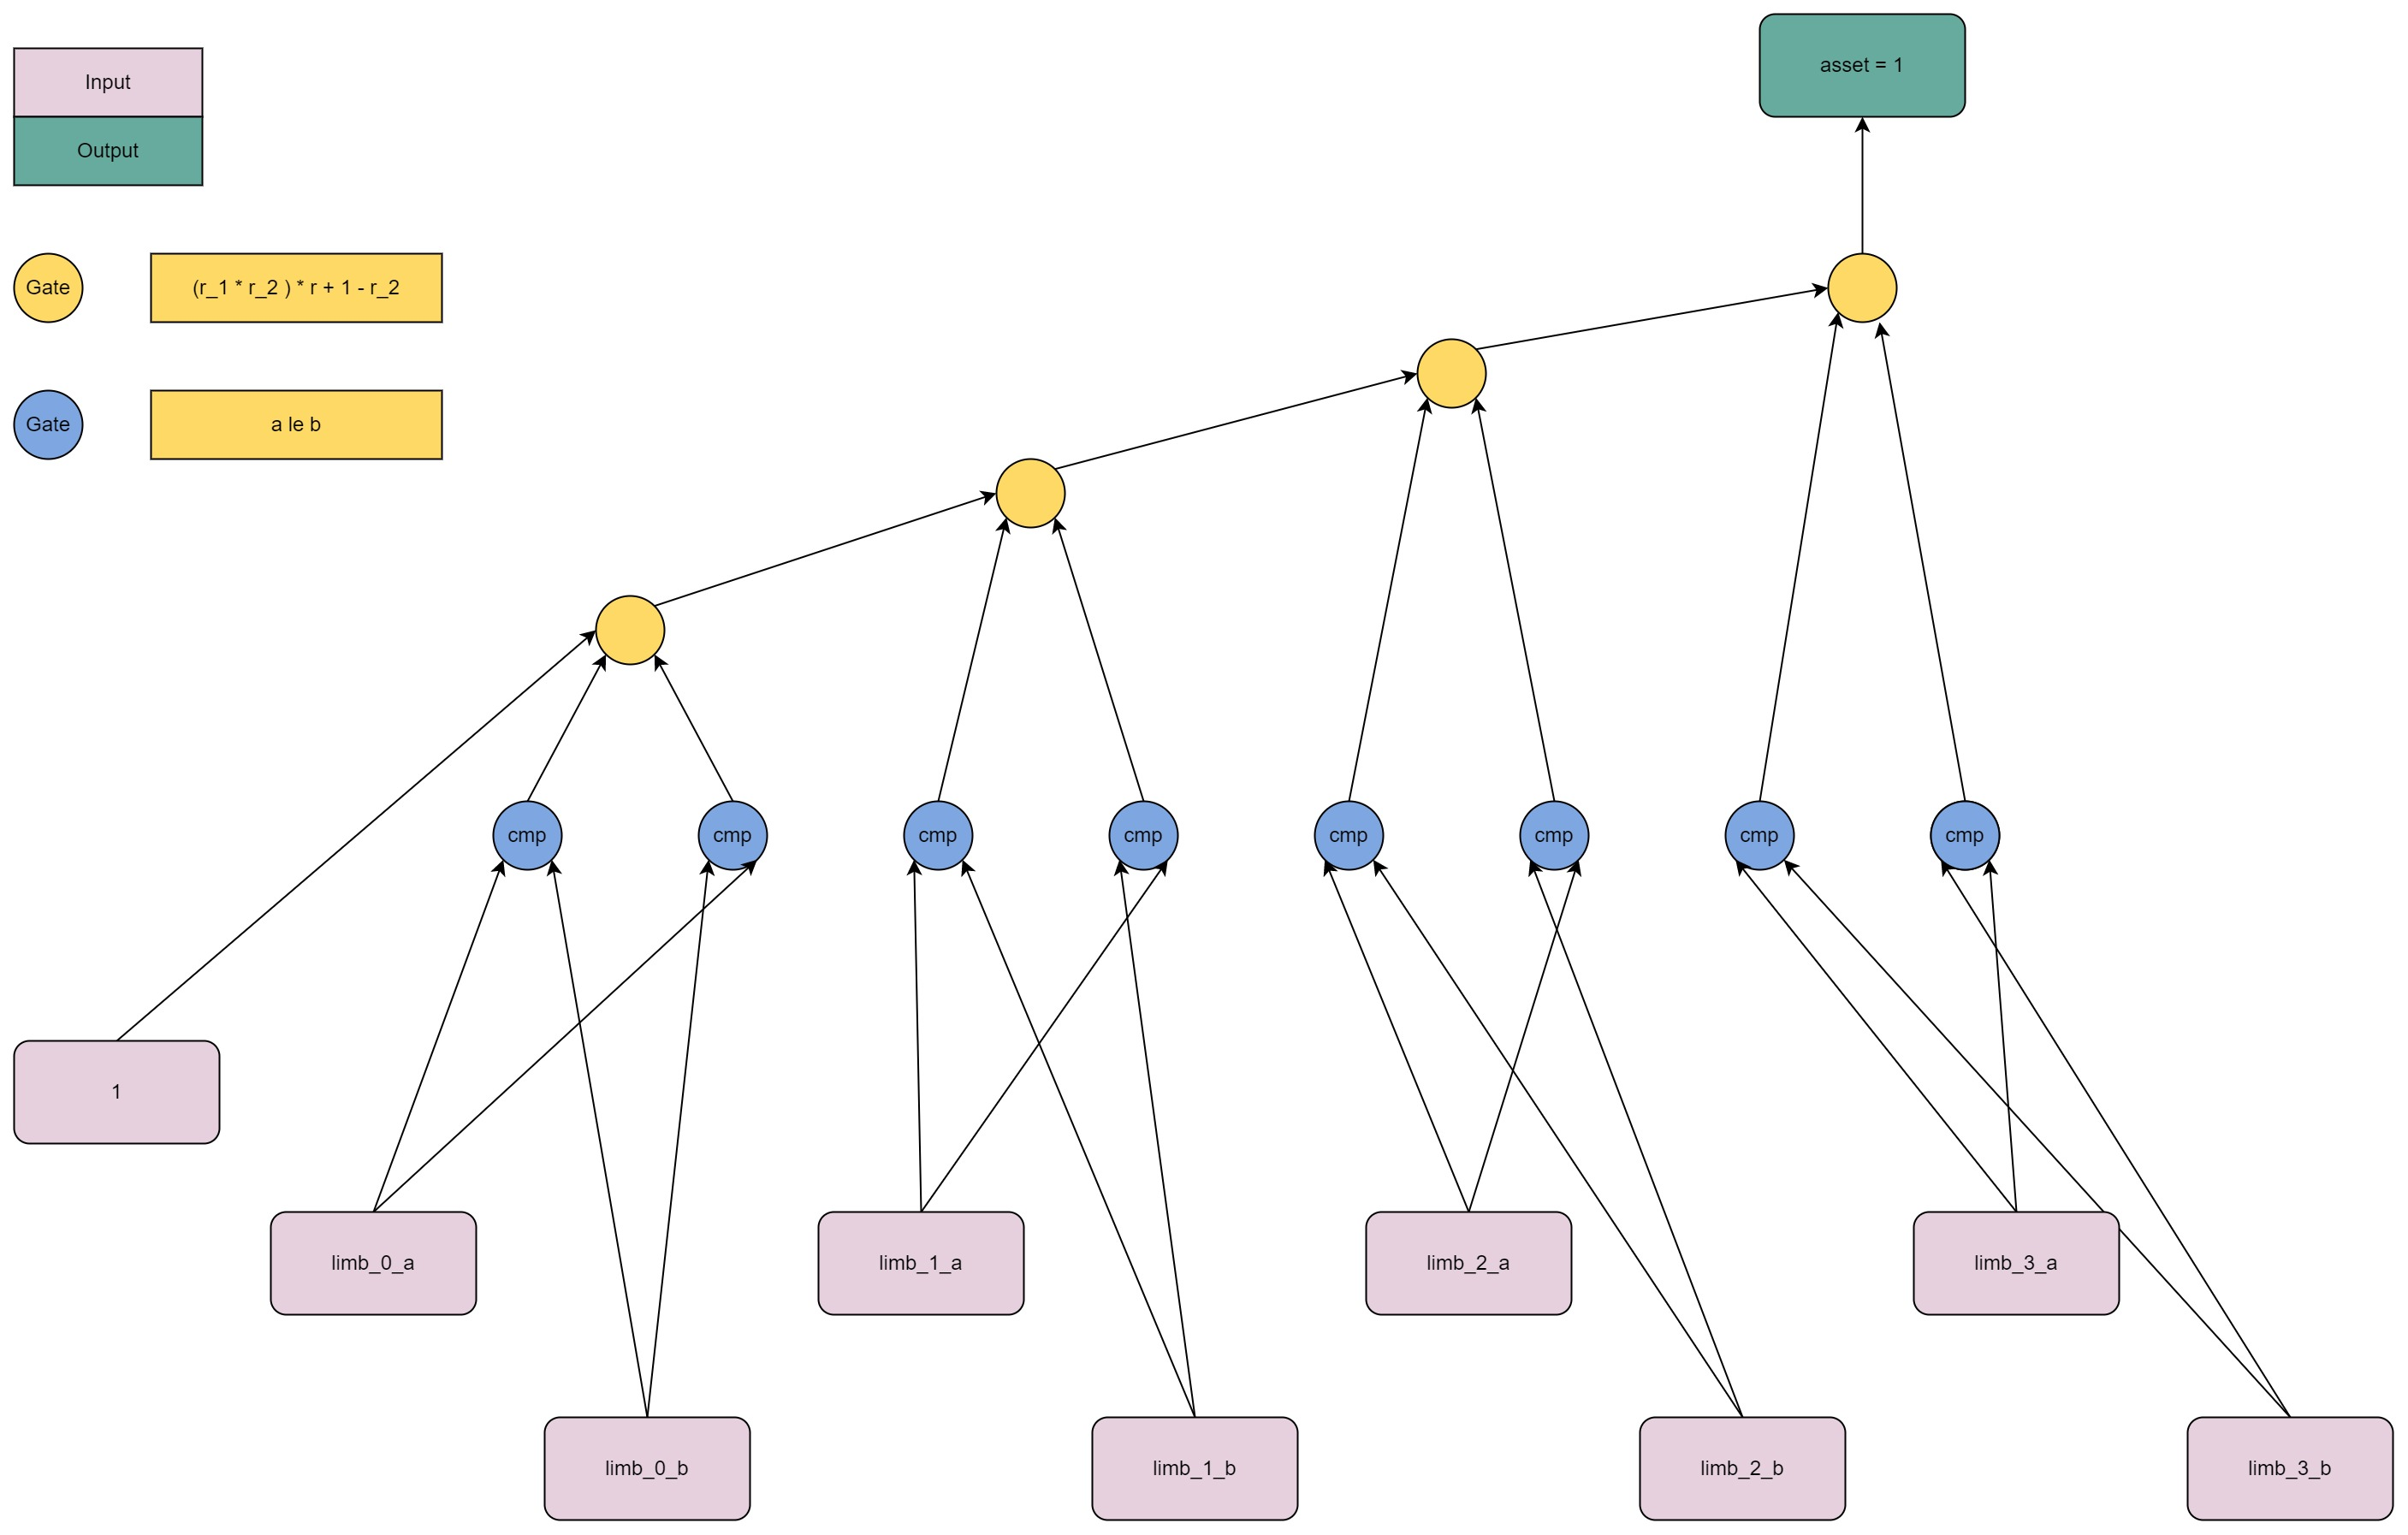
\includegraphics[width=0.8\textwidth]{biguint-cmp-circuit-layout.jpg}
    \caption{biguint-cmp circuit layout}
    \label{fig:biguint-cmp-circuit-layout}
\end{figure}

\Par{Constraints info and costs}
\begin{itemize}
    \item Gate type num: 2 (ComparisionGate, ArithmeticGate)
    \item Gate instance num: $4 \times 2 + 3 = 11$
    \item ComparisionGate num: 8
    \item ArithmeticGate num: 3
    \item copy-constraints: $(4 + 9) \times 4 + 1 = 53$
    \item max-degree: 4
\end{itemize}

    \subsubsection{nonnative-add}
\label{nonnative-add}

\begin{enumerate}
    \item target
        check the additional relation among three nonnative target objects.
    \item constraints-logic
        \begin{itemize}
            \item check equation for gadget,  a + b = c + modular * overflow
            \item check that "c lt modular"
        \end{itemize}
    \item nonnative-add process layout
        \begin{figure}[!ht]
            \centering
            \includegraphics[width=0.8\textwidth]{nonnative-add-layout.jpg}
            \caption{nonnative-add layout}
            \label{fig:nonnative-add-layout}
        \end{figure}
    
    \item constraints-info and costs
        \begin{itemize}
            \item gadget biguint-add num: 2
            \item gadget biguint-mul-by-bool num: 1
            \item gadget biguint-cmp num: 1
            \item gate type num: 3(U32AddManyGate, ComparisonGate, ArithmeticGate)
            \item gate instance num: 23 = 3(U32AddManyGate) + 16(ComparisonGate) + 2(ArithmeticGate(1,0)) + 1(ArithmeticGate(1,-1)) + 1(ArithmeticGate(1,1))
            \item copy-constraints: 186 = 32 * 2{biguint-add} + 9{biguint-mul-by-bool} + 9 + (4 + 9) * 8{biguint-cmp} = 186
        \end{itemize}

    \item questions
        \begin{itemize}
            \item when set value to sum?
        \end{itemize}

\end{enumerate}
    \subsubsection{nonnative-sub}
\label{nonnative-sub}

\begin{enumerate}
    \item target
        check the substract relation among three nonnative target objects.
    \item constraints-logic
        \begin{itemize}
            \item check equation for gadget,  diff + b = a + modular * overflow
            \item check that "overflow is bool"
            \item check that "diff.limbs is range U32"
        \end{itemize}
    \item nonnative-sub process layout
        \begin{figure}[!ht]
            \centering
            \includegraphics[width=0.8\textwidth]{nonnative-sub-layout.jpg}
            \caption{nonnative-sub layout}
            \label{fig:nonnative-sub-layout}
        \end{figure}
    
    \item constraints-info and costs
        \begin{itemize}
            \item gadget biguint-add num: 1
            \item gadget biguint-sub num: 1
            \item gadget biguint-mul-by-bool num: 1
            \item gadget u32rangecheck num: 1
            \item gadget assert-bool num: 1
            \item gate type num: 4(U32AddManyGate, U32SubtractionGate, U32RangeCheckGate, ArithmeticGate)
            \item gate instance num: 7 = 2(U32AddManyGate) + 2(U32SubtractionGate) + 1(U32RangeCheckGate) + 1(ArithmeticGate(1,0)) + 1(ArithmeticGate(1,-1))
            \item copy-constraints: 89 = 32{biguint-add num} + 27{U32SubtractionGate} + 9{biguint-mul-by-bool} + 8{u32rangecheck} + 4{assert-bool} + 9
        \end{itemize}

    \item questions
        \begin{itemize}
            \item why not constraint for overflow at nonnative-add?
            \item why not make u32rangecheck for input at nonnative-add?
        \end{itemize}

\end{enumerate}
    \subsubsection{nonnative-mul}
\label{nonnative-mul}

\begin{enumerate}
    \item target
        check the multiplicatipn relation among three nonnative target objects.
    \item constraints-logic
        \begin{itemize}
            \item check equation for gadget,  a * b = prod + modular * overflow
            \item check that "overflow.limb is U32"
            \item check that "prod.limb is U32"
        \end{itemize}
    \item nonnative-mul process layout
        \begin{figure}[!ht]
            \centering
            \includegraphics[width=0.8\textwidth]{nonnative-mul-layout.jpg}
            \caption{nonnative-mul layout}
            \label{fig:nonnative-mul-layout}
        \end{figure}
    
    \item constraints-info and costs
        \begin{itemize}
            \item gadget biguint-add num: 1
            \item gadget biguint-mul num: 2
            \item gadget u32rangecheck num: 2
            \item gate type num: 9 = 7(U32AddManyGate{3,5,7,9,11,13,15}) + 1(U32RangeCheckGate) + 1(U32ArithmeticGate)
            \item gate instance num: 37 = 2(u32rangecheck) + 8(biguint-mul: constant-input) + 22(biguint-mul) + 1 + 3(biguint-add)
            \item copy-constraints: 583 = 8 * 2(u32rangecheck) + 3 * 3 + (4 + 6 + 8 + 10 + 12 + 14 + 16) * 4 + (8 * 8) * 3 + 17 * 4 + 18
        \end{itemize}

\end{enumerate}
    \subsubsection{nonnative-inv}

\Par{Target}
Check the modular inverse relation among three nonnative target objects.

\Par{Constraints logic}
\begin{itemize}
    \item Check equation for gadget: \verb|a * inv_a = 1 + modular * div|.
\end{itemize}

\Par{Process layout}
See \figref{fig:nonnative-inv-layout}.
\begin{figure}[!ht]
    \centering
    \includegraphics[width=0.8\textwidth]{nonnative-inv-layout.jpg}
    \caption{nonnative-inv layout}
    \label{fig:nonnative-inv-layout}
\end{figure}

\Par{Constraints info and costs}
\begin{itemize}
    \item gadget biguint-add num: 1
    \item gadget biguint-mul num: 2
    \item gate type num: 8 = 7(U32AddManyGate\{3,5,7,9,11,13,15\}) + 1(U32ArithmeticGate)
    \item gate instance num: 56 = (8 * 8 + 2) * 2 / 3 + 5(U32AddManyGate{3}) + 5 + 2(U32AddManyGate{15})
    \item copy-constraints: 762 = (8 * 8 + 2) * 2 * 3 + 21 * 4 + (6 + 8 + 10 + 12 + 14) * 4 + 4 * 16 + 18
\end{itemize}

    \section{curve-add}
\label{curve-add}

Take curve-secp256k1 as example, the same as other texs.

\begin{enumerate}
    \item target
        implement the addition of two different curve points. this is a incomplete addition, you can refer to The halo2 Book \cite{website:halo2-book} to learn more about it.
    \item constraints-logic
        \begin{figure}[!ht]
            \centering
            \includegraphics[width=0.8\textwidth]{curve-add.jpg}
            \caption{curve-add}
            \label{fig:curve-add}
        \end{figure}
    \item curve-add process layout
        \begin{figure}[!ht]
            \centering
            \includegraphics[width=0.8\textwidth]{curve-add-layout.jpg}
            \caption{curve-add layout}
            \label{fig:curve-add-layout}
        \end{figure}
    
    \item constraints-info and costs
        \begin{itemize}
            \item gadget-sub-nonnative num: 5
            \item gadget-add-nonnative num: 1
            \item gadget-mul-nonnative num: 3
            \item gadget-inv-nonnative num: 1
            \item gate type num: 
            \item gate instance num: 
        \end{itemize}

\end{enumerate}
    %\printbibliography[heading=bibintoc, title=\ebibname]%
\end{document}

    \documentclass{elegantpaper}
\usepackage{datetime2}
\usepackage[T1]{fontenc}
\usepackage{graphicx}
\usepackage{listings}

\DTMusemodule{english}{en-GB}
\DTMnewdatestyle{short}{
  \renewcommand{\DTMdisplaydate}[4]{
    \DTMenglishmonthname{##2} \number##1\relax
  }
  \renewcommand{\DTMDisplaydate}{\DTMdisplaydate}
}
\newcommand{\shorttoday}{{\DTMsetdatestyle{short}\today}}
\renewcommand{\updatetext}{}

\graphicspath{{./images/}}
\DeclareEmphSequence{\bfseries,\itshape,\upshape}

\title{}
\author{Sin7Y, Applied R\&D Team\thanks{\url{https://twitter.com/Sin7Y_Labs}}}
\date{\shorttoday}

\begin{document}
    \maketitle
    \tableofcontents
    \documentclass{elegantpaper}
\usepackage{datetime2}
\usepackage[T1]{fontenc}
\usepackage{graphicx}
\usepackage{listings}

\DTMusemodule{english}{en-GB}
\DTMnewdatestyle{short}{
  \renewcommand{\DTMdisplaydate}[4]{
    \DTMenglishmonthname{##2} \number##1\relax
  }
  \renewcommand{\DTMDisplaydate}{\DTMdisplaydate}
}
\newcommand{\shorttoday}{{\DTMsetdatestyle{short}\today}}
\renewcommand{\updatetext}{}

\graphicspath{{./images/}}
\DeclareEmphSequence{\bfseries,\itshape,\upshape}

\title{}
\author{Sin7Y, Applied R\&D Team\thanks{\url{https://twitter.com/Sin7Y_Labs}}}
\date{\shorttoday}

\begin{document}
    \maketitle
    \tableofcontents
    \documentclass{elegantpaper}
\usepackage{datetime2}
\usepackage[T1]{fontenc}
\usepackage{graphicx}
\usepackage{listings}

\DTMusemodule{english}{en-GB}
\DTMnewdatestyle{short}{
  \renewcommand{\DTMdisplaydate}[4]{
    \DTMenglishmonthname{##2} \number##1\relax
  }
  \renewcommand{\DTMDisplaydate}{\DTMdisplaydate}
}
\newcommand{\shorttoday}{{\DTMsetdatestyle{short}\today}}
\renewcommand{\updatetext}{}

\graphicspath{{./images/}}
\DeclareEmphSequence{\bfseries,\itshape,\upshape}

\title{}
\author{Sin7Y, Applied R\&D Team\thanks{\url{https://twitter.com/Sin7Y_Labs}}}
\date{\shorttoday}

\begin{document}
    \maketitle
    \tableofcontents
    \input{gates/main}
    \input{gadgets/biguint/biguint-add}
    \input{gadgets/biguint/biguint-sub}
    \input{gadgets/biguint/biguint-mul}
    \input{gadgets/biguint/biguint-div}
    \input{gadgets/biguint/biguint-cmp}
    \input{gadgets/nonnative/nonnative-add}
    \input{gadgets/nonnative/nonnative-sub}
    \input{gadgets/nonnative/nonnative-mul}
    \input{gadgets/nonnative/nonnative-inv}
    \input{gadgets/curve/curve-add}
    %\printbibliography[heading=bibintoc, title=\ebibname]%
\end{document}

    \subsubsection{biguint-add}

\Par{Target}
Implement the addition of two biguints.

\Par{Constraints logic}
\begin{itemize}
    \item Equation for gates;
    \item Sumcheck between output and limbs;
    \item Rangecheck for limbs.
\end{itemize}

\Par{Circuit layout}
See \figref{fig:biguint-add-circuit-layout}.
\begin{figure}[!ht]
    \centering
    \includegraphics[width=0.8\textwidth]{biguint-add-circuit-layout.jpg}
    \caption{biguint-add circuit layout}
    \label{fig:biguint-add-circuit-layout}
\end{figure}

\Par{Trace layout}
See \figref{fig:biguint-add-trace-layout}.
\begin{figure}[!ht]
    \centering
    \includegraphics[width=0.8\textwidth]{biguint-add-trace-layout.jpg}
    \caption{biguint-add trace layout}
    \label{fig:biguint-add-trace-layout}
\end{figure}

\Par{Constraints info and costs}
\begin{itemize}
    \item gate type num: 1 (U32AddManyGate)
    \item gate ops num: limbs-num
    \item gate instance num: ceil(limbs-num / gate.ops)
    \item copy-constraints: limbs-num * 4
    \item max-degree: 4 (\verb|1 << limb-bits|)
\end{itemize}

\Par{Questions}
\begin{itemize}
    \item Why not make rangecheck constraint for inputs?
    \item Why not make copy constraint between cur-c-in and last-c-out?
\end{itemize}

    \subsubsection{biguint-sub}

\Par{Target}
Implement the substraction of two biguints.

\Par{Constraints logic}
\begin{itemize}
    \item Equation for gate;
    \item Sumcheck for ouptput;
    \item Rangecheck for limbs.
\end{itemize}

\Par{Circuit layout}
See \figref{fig:biguint-sub-circuit-layout}.
\begin{figure}[!ht]
    \centering
    \includegraphics[width=0.8\textwidth]{biguint-sub-circuit-layout.jpg}
    \caption{biguint-sub circuit layout}
    \label{fig:biguint-sub-circuit-layout}
\end{figure}

\Par{Trace layout}
See \figref{fig:biguint-sub-trace-layout}.
\begin{figure}[!ht]
    \centering
    \includegraphics[width=0.8\textwidth]{biguint-sub-trace-layout.jpg}
    \caption{biguint-sub trace layout}
    \label{fig:biguint-sub-trace-layout}
\end{figure}

\Par{Constraints info and costs}
\begin{itemize}
    \item constraints-num: $6 \times (3 + 32 / 2) = 114$
    \item copy-constraints: $16$
    \item max-degree: $4$
    \item wires-num: $6 \times (5 + 16) = 126$
\end{itemize}

\Par{Questions}
\begin{itemize}
    \item Why not make rangecheck constraint for inputs?
    \item Could try to use the same constraint with add-gate.
\end{itemize}

    \subsubsection{biguint-mul}

\Par{Target}
Implement the multiplication of two biguints.

\Par{Constraints logic}
\begin{itemize}
    \item Compute mul-factors first, use U32ArithmeticGate;
    \item Add mul-factors from low bits, use U32AddManyGate.
\end{itemize}

\Par{Process layout}
See \figref{fig:biguint-mul-layout}
\begin{figure}[!ht]
    \centering
    \includegraphics[width=0.8\textwidth]{biguint-mul-layout.jpg}
    \caption{biguint-mul layout}
    \label{fig:biguint-mul-layout}
\end{figure}

\Par{Constraints info and costs}
\begin{itemize}
    \item Gate type num: 4 (U32ArithmeticGate, U32AddManyGate(num-addends: 4), U32AddManyGate(num-addends: 6), U32AddManyGate(num-addends: 8))
    \item Gate instance num: 9
    \item U32ArithmeticGate num: 6
    \item U32AddManyGate num: 3
    \item copy-constraints: $18 \times 3 + (4 + 6 + 8) \times 2 + 9 = 99$
    \item max-degree: 4
\end{itemize}

    \section{biguint-div}
\label{biguint-div}

Note that div-rem has the same constraints logic with div

\begin{enumerate}
    \item target
        \begin{itemize}
            \item implement the division of two biguints
        \end{itemize}
    \item constraints-logic
        \begin{itemize}
            \item not implement div-algrithem directly
            \item use nondeterministic feature to check div-logic
            \item check div * b + rem = a
            \item check rem < b
        \end{itemize}
    \item div-process layout
        \begin{figure}[!ht]
            \centering
            \includegraphics[width=0.8\textwidth]{biguint-div-layout.jpg}
            \caption{biguint-div layout.jpg}
            \label{fig:biguint-div-layout.jpg}
        \end{figure}
    
    \item constraints-info and costs
        \begin{itemize}
            \item Gate type num: 5(U32ArithmeticGate, U32AddManyGate(num-addends: 3), U32AddManyGate(num-addends: 4), ComparisionGate, ArithmeticGate)
            \item Gate instance num: 3 + 3 + 4 + 3 = 13 
            \item U32ArithmeticGate num: 3
            \item U32AddManyGate num: 3
            \item ComparisionGate num: 4
            \item ArithmeticGate num: 3
            \item copy-constraints: 3 * 8 + 4 + 5 + 4 + 4 * 6 + 7 + 1 + 26 + 5 = 100 
            \item max-degree: 4
        \end{itemize}

\end{enumerate}
    \subsubsection{biguint-cmp}

\Par{Target}
Implement the comparison of two biguints.

\Par{Constraints logic}
\begin{itemize}
    \item Split the input to many limbs, such that: \verb|limbs_num = bits / chunks|;
    \item Execute comparison for low bits limbs;
    \item Ensure that the result is determined by the highest limbs which are not equal.
\end{itemize}

\Par{Process layout}
See \figref{fig:biguint-cmp-layout}.
\begin{figure}[!ht]
    \centering
    \includegraphics[width=0.8\textwidth]{biguint-cmp-layout.jpg}
    \caption{biguint-cmp layout}
    \label{fig:biguint-cmp-layout}
\end{figure}

\Par{Circuit layout}
See \figref{fig:biguint-cmp-circuit-layout}.
\begin{figure}[!ht]
    \centering
    \includegraphics[width=0.8\textwidth]{biguint-cmp-circuit-layout.jpg}
    \caption{biguint-cmp circuit layout}
    \label{fig:biguint-cmp-circuit-layout}
\end{figure}

\Par{Constraints info and costs}
\begin{itemize}
    \item Gate type num: 2 (ComparisionGate, ArithmeticGate)
    \item Gate instance num: $4 \times 2 + 3 = 11$
    \item ComparisionGate num: 8
    \item ArithmeticGate num: 3
    \item copy-constraints: $(4 + 9) \times 4 + 1 = 53$
    \item max-degree: 4
\end{itemize}

    \subsubsection{nonnative-add}
\label{nonnative-add}

\begin{enumerate}
    \item target
        check the additional relation among three nonnative target objects.
    \item constraints-logic
        \begin{itemize}
            \item check equation for gadget,  a + b = c + modular * overflow
            \item check that "c lt modular"
        \end{itemize}
    \item nonnative-add process layout
        \begin{figure}[!ht]
            \centering
            \includegraphics[width=0.8\textwidth]{nonnative-add-layout.jpg}
            \caption{nonnative-add layout}
            \label{fig:nonnative-add-layout}
        \end{figure}
    
    \item constraints-info and costs
        \begin{itemize}
            \item gadget biguint-add num: 2
            \item gadget biguint-mul-by-bool num: 1
            \item gadget biguint-cmp num: 1
            \item gate type num: 3(U32AddManyGate, ComparisonGate, ArithmeticGate)
            \item gate instance num: 23 = 3(U32AddManyGate) + 16(ComparisonGate) + 2(ArithmeticGate(1,0)) + 1(ArithmeticGate(1,-1)) + 1(ArithmeticGate(1,1))
            \item copy-constraints: 186 = 32 * 2{biguint-add} + 9{biguint-mul-by-bool} + 9 + (4 + 9) * 8{biguint-cmp} = 186
        \end{itemize}

    \item questions
        \begin{itemize}
            \item when set value to sum?
        \end{itemize}

\end{enumerate}
    \subsubsection{nonnative-sub}
\label{nonnative-sub}

\begin{enumerate}
    \item target
        check the substract relation among three nonnative target objects.
    \item constraints-logic
        \begin{itemize}
            \item check equation for gadget,  diff + b = a + modular * overflow
            \item check that "overflow is bool"
            \item check that "diff.limbs is range U32"
        \end{itemize}
    \item nonnative-sub process layout
        \begin{figure}[!ht]
            \centering
            \includegraphics[width=0.8\textwidth]{nonnative-sub-layout.jpg}
            \caption{nonnative-sub layout}
            \label{fig:nonnative-sub-layout}
        \end{figure}
    
    \item constraints-info and costs
        \begin{itemize}
            \item gadget biguint-add num: 1
            \item gadget biguint-sub num: 1
            \item gadget biguint-mul-by-bool num: 1
            \item gadget u32rangecheck num: 1
            \item gadget assert-bool num: 1
            \item gate type num: 4(U32AddManyGate, U32SubtractionGate, U32RangeCheckGate, ArithmeticGate)
            \item gate instance num: 7 = 2(U32AddManyGate) + 2(U32SubtractionGate) + 1(U32RangeCheckGate) + 1(ArithmeticGate(1,0)) + 1(ArithmeticGate(1,-1))
            \item copy-constraints: 89 = 32{biguint-add num} + 27{U32SubtractionGate} + 9{biguint-mul-by-bool} + 8{u32rangecheck} + 4{assert-bool} + 9
        \end{itemize}

    \item questions
        \begin{itemize}
            \item why not constraint for overflow at nonnative-add?
            \item why not make u32rangecheck for input at nonnative-add?
        \end{itemize}

\end{enumerate}
    \subsubsection{nonnative-mul}
\label{nonnative-mul}

\begin{enumerate}
    \item target
        check the multiplicatipn relation among three nonnative target objects.
    \item constraints-logic
        \begin{itemize}
            \item check equation for gadget,  a * b = prod + modular * overflow
            \item check that "overflow.limb is U32"
            \item check that "prod.limb is U32"
        \end{itemize}
    \item nonnative-mul process layout
        \begin{figure}[!ht]
            \centering
            \includegraphics[width=0.8\textwidth]{nonnative-mul-layout.jpg}
            \caption{nonnative-mul layout}
            \label{fig:nonnative-mul-layout}
        \end{figure}
    
    \item constraints-info and costs
        \begin{itemize}
            \item gadget biguint-add num: 1
            \item gadget biguint-mul num: 2
            \item gadget u32rangecheck num: 2
            \item gate type num: 9 = 7(U32AddManyGate{3,5,7,9,11,13,15}) + 1(U32RangeCheckGate) + 1(U32ArithmeticGate)
            \item gate instance num: 37 = 2(u32rangecheck) + 8(biguint-mul: constant-input) + 22(biguint-mul) + 1 + 3(biguint-add)
            \item copy-constraints: 583 = 8 * 2(u32rangecheck) + 3 * 3 + (4 + 6 + 8 + 10 + 12 + 14 + 16) * 4 + (8 * 8) * 3 + 17 * 4 + 18
        \end{itemize}

\end{enumerate}
    \subsubsection{nonnative-inv}

\Par{Target}
Check the modular inverse relation among three nonnative target objects.

\Par{Constraints logic}
\begin{itemize}
    \item Check equation for gadget: \verb|a * inv_a = 1 + modular * div|.
\end{itemize}

\Par{Process layout}
See \figref{fig:nonnative-inv-layout}.
\begin{figure}[!ht]
    \centering
    \includegraphics[width=0.8\textwidth]{nonnative-inv-layout.jpg}
    \caption{nonnative-inv layout}
    \label{fig:nonnative-inv-layout}
\end{figure}

\Par{Constraints info and costs}
\begin{itemize}
    \item gadget biguint-add num: 1
    \item gadget biguint-mul num: 2
    \item gate type num: 8 = 7(U32AddManyGate\{3,5,7,9,11,13,15\}) + 1(U32ArithmeticGate)
    \item gate instance num: 56 = (8 * 8 + 2) * 2 / 3 + 5(U32AddManyGate{3}) + 5 + 2(U32AddManyGate{15})
    \item copy-constraints: 762 = (8 * 8 + 2) * 2 * 3 + 21 * 4 + (6 + 8 + 10 + 12 + 14) * 4 + 4 * 16 + 18
\end{itemize}

    \section{curve-add}
\label{curve-add}

Take curve-secp256k1 as example, the same as other texs.

\begin{enumerate}
    \item target
        implement the addition of two different curve points. this is a incomplete addition, you can refer to The halo2 Book \cite{website:halo2-book} to learn more about it.
    \item constraints-logic
        \begin{figure}[!ht]
            \centering
            \includegraphics[width=0.8\textwidth]{curve-add.jpg}
            \caption{curve-add}
            \label{fig:curve-add}
        \end{figure}
    \item curve-add process layout
        \begin{figure}[!ht]
            \centering
            \includegraphics[width=0.8\textwidth]{curve-add-layout.jpg}
            \caption{curve-add layout}
            \label{fig:curve-add-layout}
        \end{figure}
    
    \item constraints-info and costs
        \begin{itemize}
            \item gadget-sub-nonnative num: 5
            \item gadget-add-nonnative num: 1
            \item gadget-mul-nonnative num: 3
            \item gadget-inv-nonnative num: 1
            \item gate type num: 
            \item gate instance num: 
        \end{itemize}

\end{enumerate}
    %\printbibliography[heading=bibintoc, title=\ebibname]%
\end{document}

    \subsubsection{biguint-add}

\Par{Target}
Implement the addition of two biguints.

\Par{Constraints logic}
\begin{itemize}
    \item Equation for gates;
    \item Sumcheck between output and limbs;
    \item Rangecheck for limbs.
\end{itemize}

\Par{Circuit layout}
See \figref{fig:biguint-add-circuit-layout}.
\begin{figure}[!ht]
    \centering
    \includegraphics[width=0.8\textwidth]{biguint-add-circuit-layout.jpg}
    \caption{biguint-add circuit layout}
    \label{fig:biguint-add-circuit-layout}
\end{figure}

\Par{Trace layout}
See \figref{fig:biguint-add-trace-layout}.
\begin{figure}[!ht]
    \centering
    \includegraphics[width=0.8\textwidth]{biguint-add-trace-layout.jpg}
    \caption{biguint-add trace layout}
    \label{fig:biguint-add-trace-layout}
\end{figure}

\Par{Constraints info and costs}
\begin{itemize}
    \item gate type num: 1 (U32AddManyGate)
    \item gate ops num: limbs-num
    \item gate instance num: ceil(limbs-num / gate.ops)
    \item copy-constraints: limbs-num * 4
    \item max-degree: 4 (\verb|1 << limb-bits|)
\end{itemize}

\Par{Questions}
\begin{itemize}
    \item Why not make rangecheck constraint for inputs?
    \item Why not make copy constraint between cur-c-in and last-c-out?
\end{itemize}

    \subsubsection{biguint-sub}

\Par{Target}
Implement the substraction of two biguints.

\Par{Constraints logic}
\begin{itemize}
    \item Equation for gate;
    \item Sumcheck for ouptput;
    \item Rangecheck for limbs.
\end{itemize}

\Par{Circuit layout}
See \figref{fig:biguint-sub-circuit-layout}.
\begin{figure}[!ht]
    \centering
    \includegraphics[width=0.8\textwidth]{biguint-sub-circuit-layout.jpg}
    \caption{biguint-sub circuit layout}
    \label{fig:biguint-sub-circuit-layout}
\end{figure}

\Par{Trace layout}
See \figref{fig:biguint-sub-trace-layout}.
\begin{figure}[!ht]
    \centering
    \includegraphics[width=0.8\textwidth]{biguint-sub-trace-layout.jpg}
    \caption{biguint-sub trace layout}
    \label{fig:biguint-sub-trace-layout}
\end{figure}

\Par{Constraints info and costs}
\begin{itemize}
    \item constraints-num: $6 \times (3 + 32 / 2) = 114$
    \item copy-constraints: $16$
    \item max-degree: $4$
    \item wires-num: $6 \times (5 + 16) = 126$
\end{itemize}

\Par{Questions}
\begin{itemize}
    \item Why not make rangecheck constraint for inputs?
    \item Could try to use the same constraint with add-gate.
\end{itemize}

    \subsubsection{biguint-mul}

\Par{Target}
Implement the multiplication of two biguints.

\Par{Constraints logic}
\begin{itemize}
    \item Compute mul-factors first, use U32ArithmeticGate;
    \item Add mul-factors from low bits, use U32AddManyGate.
\end{itemize}

\Par{Process layout}
See \figref{fig:biguint-mul-layout}
\begin{figure}[!ht]
    \centering
    \includegraphics[width=0.8\textwidth]{biguint-mul-layout.jpg}
    \caption{biguint-mul layout}
    \label{fig:biguint-mul-layout}
\end{figure}

\Par{Constraints info and costs}
\begin{itemize}
    \item Gate type num: 4 (U32ArithmeticGate, U32AddManyGate(num-addends: 4), U32AddManyGate(num-addends: 6), U32AddManyGate(num-addends: 8))
    \item Gate instance num: 9
    \item U32ArithmeticGate num: 6
    \item U32AddManyGate num: 3
    \item copy-constraints: $18 \times 3 + (4 + 6 + 8) \times 2 + 9 = 99$
    \item max-degree: 4
\end{itemize}

    \section{biguint-div}
\label{biguint-div}

Note that div-rem has the same constraints logic with div

\begin{enumerate}
    \item target
        \begin{itemize}
            \item implement the division of two biguints
        \end{itemize}
    \item constraints-logic
        \begin{itemize}
            \item not implement div-algrithem directly
            \item use nondeterministic feature to check div-logic
            \item check div * b + rem = a
            \item check rem < b
        \end{itemize}
    \item div-process layout
        \begin{figure}[!ht]
            \centering
            \includegraphics[width=0.8\textwidth]{biguint-div-layout.jpg}
            \caption{biguint-div layout.jpg}
            \label{fig:biguint-div-layout.jpg}
        \end{figure}
    
    \item constraints-info and costs
        \begin{itemize}
            \item Gate type num: 5(U32ArithmeticGate, U32AddManyGate(num-addends: 3), U32AddManyGate(num-addends: 4), ComparisionGate, ArithmeticGate)
            \item Gate instance num: 3 + 3 + 4 + 3 = 13 
            \item U32ArithmeticGate num: 3
            \item U32AddManyGate num: 3
            \item ComparisionGate num: 4
            \item ArithmeticGate num: 3
            \item copy-constraints: 3 * 8 + 4 + 5 + 4 + 4 * 6 + 7 + 1 + 26 + 5 = 100 
            \item max-degree: 4
        \end{itemize}

\end{enumerate}
    \subsubsection{biguint-cmp}

\Par{Target}
Implement the comparison of two biguints.

\Par{Constraints logic}
\begin{itemize}
    \item Split the input to many limbs, such that: \verb|limbs_num = bits / chunks|;
    \item Execute comparison for low bits limbs;
    \item Ensure that the result is determined by the highest limbs which are not equal.
\end{itemize}

\Par{Process layout}
See \figref{fig:biguint-cmp-layout}.
\begin{figure}[!ht]
    \centering
    \includegraphics[width=0.8\textwidth]{biguint-cmp-layout.jpg}
    \caption{biguint-cmp layout}
    \label{fig:biguint-cmp-layout}
\end{figure}

\Par{Circuit layout}
See \figref{fig:biguint-cmp-circuit-layout}.
\begin{figure}[!ht]
    \centering
    \includegraphics[width=0.8\textwidth]{biguint-cmp-circuit-layout.jpg}
    \caption{biguint-cmp circuit layout}
    \label{fig:biguint-cmp-circuit-layout}
\end{figure}

\Par{Constraints info and costs}
\begin{itemize}
    \item Gate type num: 2 (ComparisionGate, ArithmeticGate)
    \item Gate instance num: $4 \times 2 + 3 = 11$
    \item ComparisionGate num: 8
    \item ArithmeticGate num: 3
    \item copy-constraints: $(4 + 9) \times 4 + 1 = 53$
    \item max-degree: 4
\end{itemize}

    \subsubsection{nonnative-add}
\label{nonnative-add}

\begin{enumerate}
    \item target
        check the additional relation among three nonnative target objects.
    \item constraints-logic
        \begin{itemize}
            \item check equation for gadget,  a + b = c + modular * overflow
            \item check that "c lt modular"
        \end{itemize}
    \item nonnative-add process layout
        \begin{figure}[!ht]
            \centering
            \includegraphics[width=0.8\textwidth]{nonnative-add-layout.jpg}
            \caption{nonnative-add layout}
            \label{fig:nonnative-add-layout}
        \end{figure}
    
    \item constraints-info and costs
        \begin{itemize}
            \item gadget biguint-add num: 2
            \item gadget biguint-mul-by-bool num: 1
            \item gadget biguint-cmp num: 1
            \item gate type num: 3(U32AddManyGate, ComparisonGate, ArithmeticGate)
            \item gate instance num: 23 = 3(U32AddManyGate) + 16(ComparisonGate) + 2(ArithmeticGate(1,0)) + 1(ArithmeticGate(1,-1)) + 1(ArithmeticGate(1,1))
            \item copy-constraints: 186 = 32 * 2{biguint-add} + 9{biguint-mul-by-bool} + 9 + (4 + 9) * 8{biguint-cmp} = 186
        \end{itemize}

    \item questions
        \begin{itemize}
            \item when set value to sum?
        \end{itemize}

\end{enumerate}
    \subsubsection{nonnative-sub}
\label{nonnative-sub}

\begin{enumerate}
    \item target
        check the substract relation among three nonnative target objects.
    \item constraints-logic
        \begin{itemize}
            \item check equation for gadget,  diff + b = a + modular * overflow
            \item check that "overflow is bool"
            \item check that "diff.limbs is range U32"
        \end{itemize}
    \item nonnative-sub process layout
        \begin{figure}[!ht]
            \centering
            \includegraphics[width=0.8\textwidth]{nonnative-sub-layout.jpg}
            \caption{nonnative-sub layout}
            \label{fig:nonnative-sub-layout}
        \end{figure}
    
    \item constraints-info and costs
        \begin{itemize}
            \item gadget biguint-add num: 1
            \item gadget biguint-sub num: 1
            \item gadget biguint-mul-by-bool num: 1
            \item gadget u32rangecheck num: 1
            \item gadget assert-bool num: 1
            \item gate type num: 4(U32AddManyGate, U32SubtractionGate, U32RangeCheckGate, ArithmeticGate)
            \item gate instance num: 7 = 2(U32AddManyGate) + 2(U32SubtractionGate) + 1(U32RangeCheckGate) + 1(ArithmeticGate(1,0)) + 1(ArithmeticGate(1,-1))
            \item copy-constraints: 89 = 32{biguint-add num} + 27{U32SubtractionGate} + 9{biguint-mul-by-bool} + 8{u32rangecheck} + 4{assert-bool} + 9
        \end{itemize}

    \item questions
        \begin{itemize}
            \item why not constraint for overflow at nonnative-add?
            \item why not make u32rangecheck for input at nonnative-add?
        \end{itemize}

\end{enumerate}
    \subsubsection{nonnative-mul}
\label{nonnative-mul}

\begin{enumerate}
    \item target
        check the multiplicatipn relation among three nonnative target objects.
    \item constraints-logic
        \begin{itemize}
            \item check equation for gadget,  a * b = prod + modular * overflow
            \item check that "overflow.limb is U32"
            \item check that "prod.limb is U32"
        \end{itemize}
    \item nonnative-mul process layout
        \begin{figure}[!ht]
            \centering
            \includegraphics[width=0.8\textwidth]{nonnative-mul-layout.jpg}
            \caption{nonnative-mul layout}
            \label{fig:nonnative-mul-layout}
        \end{figure}
    
    \item constraints-info and costs
        \begin{itemize}
            \item gadget biguint-add num: 1
            \item gadget biguint-mul num: 2
            \item gadget u32rangecheck num: 2
            \item gate type num: 9 = 7(U32AddManyGate{3,5,7,9,11,13,15}) + 1(U32RangeCheckGate) + 1(U32ArithmeticGate)
            \item gate instance num: 37 = 2(u32rangecheck) + 8(biguint-mul: constant-input) + 22(biguint-mul) + 1 + 3(biguint-add)
            \item copy-constraints: 583 = 8 * 2(u32rangecheck) + 3 * 3 + (4 + 6 + 8 + 10 + 12 + 14 + 16) * 4 + (8 * 8) * 3 + 17 * 4 + 18
        \end{itemize}

\end{enumerate}
    \subsubsection{nonnative-inv}

\Par{Target}
Check the modular inverse relation among three nonnative target objects.

\Par{Constraints logic}
\begin{itemize}
    \item Check equation for gadget: \verb|a * inv_a = 1 + modular * div|.
\end{itemize}

\Par{Process layout}
See \figref{fig:nonnative-inv-layout}.
\begin{figure}[!ht]
    \centering
    \includegraphics[width=0.8\textwidth]{nonnative-inv-layout.jpg}
    \caption{nonnative-inv layout}
    \label{fig:nonnative-inv-layout}
\end{figure}

\Par{Constraints info and costs}
\begin{itemize}
    \item gadget biguint-add num: 1
    \item gadget biguint-mul num: 2
    \item gate type num: 8 = 7(U32AddManyGate\{3,5,7,9,11,13,15\}) + 1(U32ArithmeticGate)
    \item gate instance num: 56 = (8 * 8 + 2) * 2 / 3 + 5(U32AddManyGate{3}) + 5 + 2(U32AddManyGate{15})
    \item copy-constraints: 762 = (8 * 8 + 2) * 2 * 3 + 21 * 4 + (6 + 8 + 10 + 12 + 14) * 4 + 4 * 16 + 18
\end{itemize}

    \section{curve-add}
\label{curve-add}

Take curve-secp256k1 as example, the same as other texs.

\begin{enumerate}
    \item target
        implement the addition of two different curve points. this is a incomplete addition, you can refer to The halo2 Book \cite{website:halo2-book} to learn more about it.
    \item constraints-logic
        \begin{figure}[!ht]
            \centering
            \includegraphics[width=0.8\textwidth]{curve-add.jpg}
            \caption{curve-add}
            \label{fig:curve-add}
        \end{figure}
    \item curve-add process layout
        \begin{figure}[!ht]
            \centering
            \includegraphics[width=0.8\textwidth]{curve-add-layout.jpg}
            \caption{curve-add layout}
            \label{fig:curve-add-layout}
        \end{figure}
    
    \item constraints-info and costs
        \begin{itemize}
            \item gadget-sub-nonnative num: 5
            \item gadget-add-nonnative num: 1
            \item gadget-mul-nonnative num: 3
            \item gadget-inv-nonnative num: 1
            \item gate type num: 
            \item gate instance num: 
        \end{itemize}

\end{enumerate}
    %\printbibliography[heading=bibintoc, title=\ebibname]%
\end{document}
   
    \documentclass{elegantpaper}
\usepackage{datetime2}
\usepackage[T1]{fontenc}
\usepackage{graphicx}
\usepackage{listings}

\DTMusemodule{english}{en-GB}
\DTMnewdatestyle{short}{
  \renewcommand{\DTMdisplaydate}[4]{
    \DTMenglishmonthname{##2} \number##1\relax
  }
  \renewcommand{\DTMDisplaydate}{\DTMdisplaydate}
}
\newcommand{\shorttoday}{{\DTMsetdatestyle{short}\today}}
\renewcommand{\updatetext}{}

\graphicspath{{./images/}}
\DeclareEmphSequence{\bfseries,\itshape,\upshape}

\title{}
\author{Sin7Y, Applied R\&D Team\thanks{\url{https://twitter.com/Sin7Y_Labs}}}
\date{\shorttoday}

\begin{document}
    \maketitle
    \tableofcontents
    \documentclass{elegantpaper}
\usepackage{datetime2}
\usepackage[T1]{fontenc}
\usepackage{graphicx}
\usepackage{listings}

\DTMusemodule{english}{en-GB}
\DTMnewdatestyle{short}{
  \renewcommand{\DTMdisplaydate}[4]{
    \DTMenglishmonthname{##2} \number##1\relax
  }
  \renewcommand{\DTMDisplaydate}{\DTMdisplaydate}
}
\newcommand{\shorttoday}{{\DTMsetdatestyle{short}\today}}
\renewcommand{\updatetext}{}

\graphicspath{{./images/}}
\DeclareEmphSequence{\bfseries,\itshape,\upshape}

\title{}
\author{Sin7Y, Applied R\&D Team\thanks{\url{https://twitter.com/Sin7Y_Labs}}}
\date{\shorttoday}

\begin{document}
    \maketitle
    \tableofcontents
    \documentclass{elegantpaper}
\usepackage{datetime2}
\usepackage[T1]{fontenc}
\usepackage{graphicx}
\usepackage{listings}

\DTMusemodule{english}{en-GB}
\DTMnewdatestyle{short}{
  \renewcommand{\DTMdisplaydate}[4]{
    \DTMenglishmonthname{##2} \number##1\relax
  }
  \renewcommand{\DTMDisplaydate}{\DTMdisplaydate}
}
\newcommand{\shorttoday}{{\DTMsetdatestyle{short}\today}}
\renewcommand{\updatetext}{}

\graphicspath{{./images/}}
\DeclareEmphSequence{\bfseries,\itshape,\upshape}

\title{}
\author{Sin7Y, Applied R\&D Team\thanks{\url{https://twitter.com/Sin7Y_Labs}}}
\date{\shorttoday}

\begin{document}
    \maketitle
    \tableofcontents
    \input{gates/main}
    \input{gadgets/biguint/biguint-add}
    \input{gadgets/biguint/biguint-sub}
    \input{gadgets/biguint/biguint-mul}
    \input{gadgets/biguint/biguint-div}
    \input{gadgets/biguint/biguint-cmp}
    \input{gadgets/nonnative/nonnative-add}
    \input{gadgets/nonnative/nonnative-sub}
    \input{gadgets/nonnative/nonnative-mul}
    \input{gadgets/nonnative/nonnative-inv}
    \input{gadgets/curve/curve-add}
    %\printbibliography[heading=bibintoc, title=\ebibname]%
\end{document}

    \subsubsection{biguint-add}

\Par{Target}
Implement the addition of two biguints.

\Par{Constraints logic}
\begin{itemize}
    \item Equation for gates;
    \item Sumcheck between output and limbs;
    \item Rangecheck for limbs.
\end{itemize}

\Par{Circuit layout}
See \figref{fig:biguint-add-circuit-layout}.
\begin{figure}[!ht]
    \centering
    \includegraphics[width=0.8\textwidth]{biguint-add-circuit-layout.jpg}
    \caption{biguint-add circuit layout}
    \label{fig:biguint-add-circuit-layout}
\end{figure}

\Par{Trace layout}
See \figref{fig:biguint-add-trace-layout}.
\begin{figure}[!ht]
    \centering
    \includegraphics[width=0.8\textwidth]{biguint-add-trace-layout.jpg}
    \caption{biguint-add trace layout}
    \label{fig:biguint-add-trace-layout}
\end{figure}

\Par{Constraints info and costs}
\begin{itemize}
    \item gate type num: 1 (U32AddManyGate)
    \item gate ops num: limbs-num
    \item gate instance num: ceil(limbs-num / gate.ops)
    \item copy-constraints: limbs-num * 4
    \item max-degree: 4 (\verb|1 << limb-bits|)
\end{itemize}

\Par{Questions}
\begin{itemize}
    \item Why not make rangecheck constraint for inputs?
    \item Why not make copy constraint between cur-c-in and last-c-out?
\end{itemize}

    \subsubsection{biguint-sub}

\Par{Target}
Implement the substraction of two biguints.

\Par{Constraints logic}
\begin{itemize}
    \item Equation for gate;
    \item Sumcheck for ouptput;
    \item Rangecheck for limbs.
\end{itemize}

\Par{Circuit layout}
See \figref{fig:biguint-sub-circuit-layout}.
\begin{figure}[!ht]
    \centering
    \includegraphics[width=0.8\textwidth]{biguint-sub-circuit-layout.jpg}
    \caption{biguint-sub circuit layout}
    \label{fig:biguint-sub-circuit-layout}
\end{figure}

\Par{Trace layout}
See \figref{fig:biguint-sub-trace-layout}.
\begin{figure}[!ht]
    \centering
    \includegraphics[width=0.8\textwidth]{biguint-sub-trace-layout.jpg}
    \caption{biguint-sub trace layout}
    \label{fig:biguint-sub-trace-layout}
\end{figure}

\Par{Constraints info and costs}
\begin{itemize}
    \item constraints-num: $6 \times (3 + 32 / 2) = 114$
    \item copy-constraints: $16$
    \item max-degree: $4$
    \item wires-num: $6 \times (5 + 16) = 126$
\end{itemize}

\Par{Questions}
\begin{itemize}
    \item Why not make rangecheck constraint for inputs?
    \item Could try to use the same constraint with add-gate.
\end{itemize}

    \subsubsection{biguint-mul}

\Par{Target}
Implement the multiplication of two biguints.

\Par{Constraints logic}
\begin{itemize}
    \item Compute mul-factors first, use U32ArithmeticGate;
    \item Add mul-factors from low bits, use U32AddManyGate.
\end{itemize}

\Par{Process layout}
See \figref{fig:biguint-mul-layout}
\begin{figure}[!ht]
    \centering
    \includegraphics[width=0.8\textwidth]{biguint-mul-layout.jpg}
    \caption{biguint-mul layout}
    \label{fig:biguint-mul-layout}
\end{figure}

\Par{Constraints info and costs}
\begin{itemize}
    \item Gate type num: 4 (U32ArithmeticGate, U32AddManyGate(num-addends: 4), U32AddManyGate(num-addends: 6), U32AddManyGate(num-addends: 8))
    \item Gate instance num: 9
    \item U32ArithmeticGate num: 6
    \item U32AddManyGate num: 3
    \item copy-constraints: $18 \times 3 + (4 + 6 + 8) \times 2 + 9 = 99$
    \item max-degree: 4
\end{itemize}

    \section{biguint-div}
\label{biguint-div}

Note that div-rem has the same constraints logic with div

\begin{enumerate}
    \item target
        \begin{itemize}
            \item implement the division of two biguints
        \end{itemize}
    \item constraints-logic
        \begin{itemize}
            \item not implement div-algrithem directly
            \item use nondeterministic feature to check div-logic
            \item check div * b + rem = a
            \item check rem < b
        \end{itemize}
    \item div-process layout
        \begin{figure}[!ht]
            \centering
            \includegraphics[width=0.8\textwidth]{biguint-div-layout.jpg}
            \caption{biguint-div layout.jpg}
            \label{fig:biguint-div-layout.jpg}
        \end{figure}
    
    \item constraints-info and costs
        \begin{itemize}
            \item Gate type num: 5(U32ArithmeticGate, U32AddManyGate(num-addends: 3), U32AddManyGate(num-addends: 4), ComparisionGate, ArithmeticGate)
            \item Gate instance num: 3 + 3 + 4 + 3 = 13 
            \item U32ArithmeticGate num: 3
            \item U32AddManyGate num: 3
            \item ComparisionGate num: 4
            \item ArithmeticGate num: 3
            \item copy-constraints: 3 * 8 + 4 + 5 + 4 + 4 * 6 + 7 + 1 + 26 + 5 = 100 
            \item max-degree: 4
        \end{itemize}

\end{enumerate}
    \subsubsection{biguint-cmp}

\Par{Target}
Implement the comparison of two biguints.

\Par{Constraints logic}
\begin{itemize}
    \item Split the input to many limbs, such that: \verb|limbs_num = bits / chunks|;
    \item Execute comparison for low bits limbs;
    \item Ensure that the result is determined by the highest limbs which are not equal.
\end{itemize}

\Par{Process layout}
See \figref{fig:biguint-cmp-layout}.
\begin{figure}[!ht]
    \centering
    \includegraphics[width=0.8\textwidth]{biguint-cmp-layout.jpg}
    \caption{biguint-cmp layout}
    \label{fig:biguint-cmp-layout}
\end{figure}

\Par{Circuit layout}
See \figref{fig:biguint-cmp-circuit-layout}.
\begin{figure}[!ht]
    \centering
    \includegraphics[width=0.8\textwidth]{biguint-cmp-circuit-layout.jpg}
    \caption{biguint-cmp circuit layout}
    \label{fig:biguint-cmp-circuit-layout}
\end{figure}

\Par{Constraints info and costs}
\begin{itemize}
    \item Gate type num: 2 (ComparisionGate, ArithmeticGate)
    \item Gate instance num: $4 \times 2 + 3 = 11$
    \item ComparisionGate num: 8
    \item ArithmeticGate num: 3
    \item copy-constraints: $(4 + 9) \times 4 + 1 = 53$
    \item max-degree: 4
\end{itemize}

    \subsubsection{nonnative-add}
\label{nonnative-add}

\begin{enumerate}
    \item target
        check the additional relation among three nonnative target objects.
    \item constraints-logic
        \begin{itemize}
            \item check equation for gadget,  a + b = c + modular * overflow
            \item check that "c lt modular"
        \end{itemize}
    \item nonnative-add process layout
        \begin{figure}[!ht]
            \centering
            \includegraphics[width=0.8\textwidth]{nonnative-add-layout.jpg}
            \caption{nonnative-add layout}
            \label{fig:nonnative-add-layout}
        \end{figure}
    
    \item constraints-info and costs
        \begin{itemize}
            \item gadget biguint-add num: 2
            \item gadget biguint-mul-by-bool num: 1
            \item gadget biguint-cmp num: 1
            \item gate type num: 3(U32AddManyGate, ComparisonGate, ArithmeticGate)
            \item gate instance num: 23 = 3(U32AddManyGate) + 16(ComparisonGate) + 2(ArithmeticGate(1,0)) + 1(ArithmeticGate(1,-1)) + 1(ArithmeticGate(1,1))
            \item copy-constraints: 186 = 32 * 2{biguint-add} + 9{biguint-mul-by-bool} + 9 + (4 + 9) * 8{biguint-cmp} = 186
        \end{itemize}

    \item questions
        \begin{itemize}
            \item when set value to sum?
        \end{itemize}

\end{enumerate}
    \subsubsection{nonnative-sub}
\label{nonnative-sub}

\begin{enumerate}
    \item target
        check the substract relation among three nonnative target objects.
    \item constraints-logic
        \begin{itemize}
            \item check equation for gadget,  diff + b = a + modular * overflow
            \item check that "overflow is bool"
            \item check that "diff.limbs is range U32"
        \end{itemize}
    \item nonnative-sub process layout
        \begin{figure}[!ht]
            \centering
            \includegraphics[width=0.8\textwidth]{nonnative-sub-layout.jpg}
            \caption{nonnative-sub layout}
            \label{fig:nonnative-sub-layout}
        \end{figure}
    
    \item constraints-info and costs
        \begin{itemize}
            \item gadget biguint-add num: 1
            \item gadget biguint-sub num: 1
            \item gadget biguint-mul-by-bool num: 1
            \item gadget u32rangecheck num: 1
            \item gadget assert-bool num: 1
            \item gate type num: 4(U32AddManyGate, U32SubtractionGate, U32RangeCheckGate, ArithmeticGate)
            \item gate instance num: 7 = 2(U32AddManyGate) + 2(U32SubtractionGate) + 1(U32RangeCheckGate) + 1(ArithmeticGate(1,0)) + 1(ArithmeticGate(1,-1))
            \item copy-constraints: 89 = 32{biguint-add num} + 27{U32SubtractionGate} + 9{biguint-mul-by-bool} + 8{u32rangecheck} + 4{assert-bool} + 9
        \end{itemize}

    \item questions
        \begin{itemize}
            \item why not constraint for overflow at nonnative-add?
            \item why not make u32rangecheck for input at nonnative-add?
        \end{itemize}

\end{enumerate}
    \subsubsection{nonnative-mul}
\label{nonnative-mul}

\begin{enumerate}
    \item target
        check the multiplicatipn relation among three nonnative target objects.
    \item constraints-logic
        \begin{itemize}
            \item check equation for gadget,  a * b = prod + modular * overflow
            \item check that "overflow.limb is U32"
            \item check that "prod.limb is U32"
        \end{itemize}
    \item nonnative-mul process layout
        \begin{figure}[!ht]
            \centering
            \includegraphics[width=0.8\textwidth]{nonnative-mul-layout.jpg}
            \caption{nonnative-mul layout}
            \label{fig:nonnative-mul-layout}
        \end{figure}
    
    \item constraints-info and costs
        \begin{itemize}
            \item gadget biguint-add num: 1
            \item gadget biguint-mul num: 2
            \item gadget u32rangecheck num: 2
            \item gate type num: 9 = 7(U32AddManyGate{3,5,7,9,11,13,15}) + 1(U32RangeCheckGate) + 1(U32ArithmeticGate)
            \item gate instance num: 37 = 2(u32rangecheck) + 8(biguint-mul: constant-input) + 22(biguint-mul) + 1 + 3(biguint-add)
            \item copy-constraints: 583 = 8 * 2(u32rangecheck) + 3 * 3 + (4 + 6 + 8 + 10 + 12 + 14 + 16) * 4 + (8 * 8) * 3 + 17 * 4 + 18
        \end{itemize}

\end{enumerate}
    \subsubsection{nonnative-inv}

\Par{Target}
Check the modular inverse relation among three nonnative target objects.

\Par{Constraints logic}
\begin{itemize}
    \item Check equation for gadget: \verb|a * inv_a = 1 + modular * div|.
\end{itemize}

\Par{Process layout}
See \figref{fig:nonnative-inv-layout}.
\begin{figure}[!ht]
    \centering
    \includegraphics[width=0.8\textwidth]{nonnative-inv-layout.jpg}
    \caption{nonnative-inv layout}
    \label{fig:nonnative-inv-layout}
\end{figure}

\Par{Constraints info and costs}
\begin{itemize}
    \item gadget biguint-add num: 1
    \item gadget biguint-mul num: 2
    \item gate type num: 8 = 7(U32AddManyGate\{3,5,7,9,11,13,15\}) + 1(U32ArithmeticGate)
    \item gate instance num: 56 = (8 * 8 + 2) * 2 / 3 + 5(U32AddManyGate{3}) + 5 + 2(U32AddManyGate{15})
    \item copy-constraints: 762 = (8 * 8 + 2) * 2 * 3 + 21 * 4 + (6 + 8 + 10 + 12 + 14) * 4 + 4 * 16 + 18
\end{itemize}

    \section{curve-add}
\label{curve-add}

Take curve-secp256k1 as example, the same as other texs.

\begin{enumerate}
    \item target
        implement the addition of two different curve points. this is a incomplete addition, you can refer to The halo2 Book \cite{website:halo2-book} to learn more about it.
    \item constraints-logic
        \begin{figure}[!ht]
            \centering
            \includegraphics[width=0.8\textwidth]{curve-add.jpg}
            \caption{curve-add}
            \label{fig:curve-add}
        \end{figure}
    \item curve-add process layout
        \begin{figure}[!ht]
            \centering
            \includegraphics[width=0.8\textwidth]{curve-add-layout.jpg}
            \caption{curve-add layout}
            \label{fig:curve-add-layout}
        \end{figure}
    
    \item constraints-info and costs
        \begin{itemize}
            \item gadget-sub-nonnative num: 5
            \item gadget-add-nonnative num: 1
            \item gadget-mul-nonnative num: 3
            \item gadget-inv-nonnative num: 1
            \item gate type num: 
            \item gate instance num: 
        \end{itemize}

\end{enumerate}
    %\printbibliography[heading=bibintoc, title=\ebibname]%
\end{document}

    \subsubsection{biguint-add}

\Par{Target}
Implement the addition of two biguints.

\Par{Constraints logic}
\begin{itemize}
    \item Equation for gates;
    \item Sumcheck between output and limbs;
    \item Rangecheck for limbs.
\end{itemize}

\Par{Circuit layout}
See \figref{fig:biguint-add-circuit-layout}.
\begin{figure}[!ht]
    \centering
    \includegraphics[width=0.8\textwidth]{biguint-add-circuit-layout.jpg}
    \caption{biguint-add circuit layout}
    \label{fig:biguint-add-circuit-layout}
\end{figure}

\Par{Trace layout}
See \figref{fig:biguint-add-trace-layout}.
\begin{figure}[!ht]
    \centering
    \includegraphics[width=0.8\textwidth]{biguint-add-trace-layout.jpg}
    \caption{biguint-add trace layout}
    \label{fig:biguint-add-trace-layout}
\end{figure}

\Par{Constraints info and costs}
\begin{itemize}
    \item gate type num: 1 (U32AddManyGate)
    \item gate ops num: limbs-num
    \item gate instance num: ceil(limbs-num / gate.ops)
    \item copy-constraints: limbs-num * 4
    \item max-degree: 4 (\verb|1 << limb-bits|)
\end{itemize}

\Par{Questions}
\begin{itemize}
    \item Why not make rangecheck constraint for inputs?
    \item Why not make copy constraint between cur-c-in and last-c-out?
\end{itemize}

    \subsubsection{biguint-sub}

\Par{Target}
Implement the substraction of two biguints.

\Par{Constraints logic}
\begin{itemize}
    \item Equation for gate;
    \item Sumcheck for ouptput;
    \item Rangecheck for limbs.
\end{itemize}

\Par{Circuit layout}
See \figref{fig:biguint-sub-circuit-layout}.
\begin{figure}[!ht]
    \centering
    \includegraphics[width=0.8\textwidth]{biguint-sub-circuit-layout.jpg}
    \caption{biguint-sub circuit layout}
    \label{fig:biguint-sub-circuit-layout}
\end{figure}

\Par{Trace layout}
See \figref{fig:biguint-sub-trace-layout}.
\begin{figure}[!ht]
    \centering
    \includegraphics[width=0.8\textwidth]{biguint-sub-trace-layout.jpg}
    \caption{biguint-sub trace layout}
    \label{fig:biguint-sub-trace-layout}
\end{figure}

\Par{Constraints info and costs}
\begin{itemize}
    \item constraints-num: $6 \times (3 + 32 / 2) = 114$
    \item copy-constraints: $16$
    \item max-degree: $4$
    \item wires-num: $6 \times (5 + 16) = 126$
\end{itemize}

\Par{Questions}
\begin{itemize}
    \item Why not make rangecheck constraint for inputs?
    \item Could try to use the same constraint with add-gate.
\end{itemize}

    \subsubsection{biguint-mul}

\Par{Target}
Implement the multiplication of two biguints.

\Par{Constraints logic}
\begin{itemize}
    \item Compute mul-factors first, use U32ArithmeticGate;
    \item Add mul-factors from low bits, use U32AddManyGate.
\end{itemize}

\Par{Process layout}
See \figref{fig:biguint-mul-layout}
\begin{figure}[!ht]
    \centering
    \includegraphics[width=0.8\textwidth]{biguint-mul-layout.jpg}
    \caption{biguint-mul layout}
    \label{fig:biguint-mul-layout}
\end{figure}

\Par{Constraints info and costs}
\begin{itemize}
    \item Gate type num: 4 (U32ArithmeticGate, U32AddManyGate(num-addends: 4), U32AddManyGate(num-addends: 6), U32AddManyGate(num-addends: 8))
    \item Gate instance num: 9
    \item U32ArithmeticGate num: 6
    \item U32AddManyGate num: 3
    \item copy-constraints: $18 \times 3 + (4 + 6 + 8) \times 2 + 9 = 99$
    \item max-degree: 4
\end{itemize}

    \section{biguint-div}
\label{biguint-div}

Note that div-rem has the same constraints logic with div

\begin{enumerate}
    \item target
        \begin{itemize}
            \item implement the division of two biguints
        \end{itemize}
    \item constraints-logic
        \begin{itemize}
            \item not implement div-algrithem directly
            \item use nondeterministic feature to check div-logic
            \item check div * b + rem = a
            \item check rem < b
        \end{itemize}
    \item div-process layout
        \begin{figure}[!ht]
            \centering
            \includegraphics[width=0.8\textwidth]{biguint-div-layout.jpg}
            \caption{biguint-div layout.jpg}
            \label{fig:biguint-div-layout.jpg}
        \end{figure}
    
    \item constraints-info and costs
        \begin{itemize}
            \item Gate type num: 5(U32ArithmeticGate, U32AddManyGate(num-addends: 3), U32AddManyGate(num-addends: 4), ComparisionGate, ArithmeticGate)
            \item Gate instance num: 3 + 3 + 4 + 3 = 13 
            \item U32ArithmeticGate num: 3
            \item U32AddManyGate num: 3
            \item ComparisionGate num: 4
            \item ArithmeticGate num: 3
            \item copy-constraints: 3 * 8 + 4 + 5 + 4 + 4 * 6 + 7 + 1 + 26 + 5 = 100 
            \item max-degree: 4
        \end{itemize}

\end{enumerate}
    \subsubsection{biguint-cmp}

\Par{Target}
Implement the comparison of two biguints.

\Par{Constraints logic}
\begin{itemize}
    \item Split the input to many limbs, such that: \verb|limbs_num = bits / chunks|;
    \item Execute comparison for low bits limbs;
    \item Ensure that the result is determined by the highest limbs which are not equal.
\end{itemize}

\Par{Process layout}
See \figref{fig:biguint-cmp-layout}.
\begin{figure}[!ht]
    \centering
    \includegraphics[width=0.8\textwidth]{biguint-cmp-layout.jpg}
    \caption{biguint-cmp layout}
    \label{fig:biguint-cmp-layout}
\end{figure}

\Par{Circuit layout}
See \figref{fig:biguint-cmp-circuit-layout}.
\begin{figure}[!ht]
    \centering
    \includegraphics[width=0.8\textwidth]{biguint-cmp-circuit-layout.jpg}
    \caption{biguint-cmp circuit layout}
    \label{fig:biguint-cmp-circuit-layout}
\end{figure}

\Par{Constraints info and costs}
\begin{itemize}
    \item Gate type num: 2 (ComparisionGate, ArithmeticGate)
    \item Gate instance num: $4 \times 2 + 3 = 11$
    \item ComparisionGate num: 8
    \item ArithmeticGate num: 3
    \item copy-constraints: $(4 + 9) \times 4 + 1 = 53$
    \item max-degree: 4
\end{itemize}

    \subsubsection{nonnative-add}
\label{nonnative-add}

\begin{enumerate}
    \item target
        check the additional relation among three nonnative target objects.
    \item constraints-logic
        \begin{itemize}
            \item check equation for gadget,  a + b = c + modular * overflow
            \item check that "c lt modular"
        \end{itemize}
    \item nonnative-add process layout
        \begin{figure}[!ht]
            \centering
            \includegraphics[width=0.8\textwidth]{nonnative-add-layout.jpg}
            \caption{nonnative-add layout}
            \label{fig:nonnative-add-layout}
        \end{figure}
    
    \item constraints-info and costs
        \begin{itemize}
            \item gadget biguint-add num: 2
            \item gadget biguint-mul-by-bool num: 1
            \item gadget biguint-cmp num: 1
            \item gate type num: 3(U32AddManyGate, ComparisonGate, ArithmeticGate)
            \item gate instance num: 23 = 3(U32AddManyGate) + 16(ComparisonGate) + 2(ArithmeticGate(1,0)) + 1(ArithmeticGate(1,-1)) + 1(ArithmeticGate(1,1))
            \item copy-constraints: 186 = 32 * 2{biguint-add} + 9{biguint-mul-by-bool} + 9 + (4 + 9) * 8{biguint-cmp} = 186
        \end{itemize}

    \item questions
        \begin{itemize}
            \item when set value to sum?
        \end{itemize}

\end{enumerate}
    \subsubsection{nonnative-sub}
\label{nonnative-sub}

\begin{enumerate}
    \item target
        check the substract relation among three nonnative target objects.
    \item constraints-logic
        \begin{itemize}
            \item check equation for gadget,  diff + b = a + modular * overflow
            \item check that "overflow is bool"
            \item check that "diff.limbs is range U32"
        \end{itemize}
    \item nonnative-sub process layout
        \begin{figure}[!ht]
            \centering
            \includegraphics[width=0.8\textwidth]{nonnative-sub-layout.jpg}
            \caption{nonnative-sub layout}
            \label{fig:nonnative-sub-layout}
        \end{figure}
    
    \item constraints-info and costs
        \begin{itemize}
            \item gadget biguint-add num: 1
            \item gadget biguint-sub num: 1
            \item gadget biguint-mul-by-bool num: 1
            \item gadget u32rangecheck num: 1
            \item gadget assert-bool num: 1
            \item gate type num: 4(U32AddManyGate, U32SubtractionGate, U32RangeCheckGate, ArithmeticGate)
            \item gate instance num: 7 = 2(U32AddManyGate) + 2(U32SubtractionGate) + 1(U32RangeCheckGate) + 1(ArithmeticGate(1,0)) + 1(ArithmeticGate(1,-1))
            \item copy-constraints: 89 = 32{biguint-add num} + 27{U32SubtractionGate} + 9{biguint-mul-by-bool} + 8{u32rangecheck} + 4{assert-bool} + 9
        \end{itemize}

    \item questions
        \begin{itemize}
            \item why not constraint for overflow at nonnative-add?
            \item why not make u32rangecheck for input at nonnative-add?
        \end{itemize}

\end{enumerate}
    \subsubsection{nonnative-mul}
\label{nonnative-mul}

\begin{enumerate}
    \item target
        check the multiplicatipn relation among three nonnative target objects.
    \item constraints-logic
        \begin{itemize}
            \item check equation for gadget,  a * b = prod + modular * overflow
            \item check that "overflow.limb is U32"
            \item check that "prod.limb is U32"
        \end{itemize}
    \item nonnative-mul process layout
        \begin{figure}[!ht]
            \centering
            \includegraphics[width=0.8\textwidth]{nonnative-mul-layout.jpg}
            \caption{nonnative-mul layout}
            \label{fig:nonnative-mul-layout}
        \end{figure}
    
    \item constraints-info and costs
        \begin{itemize}
            \item gadget biguint-add num: 1
            \item gadget biguint-mul num: 2
            \item gadget u32rangecheck num: 2
            \item gate type num: 9 = 7(U32AddManyGate{3,5,7,9,11,13,15}) + 1(U32RangeCheckGate) + 1(U32ArithmeticGate)
            \item gate instance num: 37 = 2(u32rangecheck) + 8(biguint-mul: constant-input) + 22(biguint-mul) + 1 + 3(biguint-add)
            \item copy-constraints: 583 = 8 * 2(u32rangecheck) + 3 * 3 + (4 + 6 + 8 + 10 + 12 + 14 + 16) * 4 + (8 * 8) * 3 + 17 * 4 + 18
        \end{itemize}

\end{enumerate}
    \subsubsection{nonnative-inv}

\Par{Target}
Check the modular inverse relation among three nonnative target objects.

\Par{Constraints logic}
\begin{itemize}
    \item Check equation for gadget: \verb|a * inv_a = 1 + modular * div|.
\end{itemize}

\Par{Process layout}
See \figref{fig:nonnative-inv-layout}.
\begin{figure}[!ht]
    \centering
    \includegraphics[width=0.8\textwidth]{nonnative-inv-layout.jpg}
    \caption{nonnative-inv layout}
    \label{fig:nonnative-inv-layout}
\end{figure}

\Par{Constraints info and costs}
\begin{itemize}
    \item gadget biguint-add num: 1
    \item gadget biguint-mul num: 2
    \item gate type num: 8 = 7(U32AddManyGate\{3,5,7,9,11,13,15\}) + 1(U32ArithmeticGate)
    \item gate instance num: 56 = (8 * 8 + 2) * 2 / 3 + 5(U32AddManyGate{3}) + 5 + 2(U32AddManyGate{15})
    \item copy-constraints: 762 = (8 * 8 + 2) * 2 * 3 + 21 * 4 + (6 + 8 + 10 + 12 + 14) * 4 + 4 * 16 + 18
\end{itemize}

    \section{curve-add}
\label{curve-add}

Take curve-secp256k1 as example, the same as other texs.

\begin{enumerate}
    \item target
        implement the addition of two different curve points. this is a incomplete addition, you can refer to The halo2 Book \cite{website:halo2-book} to learn more about it.
    \item constraints-logic
        \begin{figure}[!ht]
            \centering
            \includegraphics[width=0.8\textwidth]{curve-add.jpg}
            \caption{curve-add}
            \label{fig:curve-add}
        \end{figure}
    \item curve-add process layout
        \begin{figure}[!ht]
            \centering
            \includegraphics[width=0.8\textwidth]{curve-add-layout.jpg}
            \caption{curve-add layout}
            \label{fig:curve-add-layout}
        \end{figure}
    
    \item constraints-info and costs
        \begin{itemize}
            \item gadget-sub-nonnative num: 5
            \item gadget-add-nonnative num: 1
            \item gadget-mul-nonnative num: 3
            \item gadget-inv-nonnative num: 1
            \item gate type num: 
            \item gate instance num: 
        \end{itemize}

\end{enumerate}
    %\printbibliography[heading=bibintoc, title=\ebibname]%
\end{document}

    %\printbibliography[heading=bibintoc, title=\ebibname]%
\end{document}
